% !TEX program = latexmk
% !TEX TS-program = pdflatexmk

\documentclass[twoside,10pt]{ttuthesis}

\lstset{basicstyle=\ttfamily}

%%% Macros for commonly-used symbols

% \ensuremath (from amsmath) so that we can use commands in regular text,
% or in math mode
% \xspace to ensure that we can easily write \DeltaK or \DeltaK-decreasing and
% not \DeltaK{} or \DeltaK{}-decreasing

\usepackage{xspace}

\newcommand{\hone}{\ensuremath{h_1}\xspace} % this is no shorter than $h_1$, but much easier to type overall. No, we can't use \h1 unless we define a command for \h that gobbles up the next block of text.
\newcommand{\htwo}{\ensuremath{h_2}\xspace}
\newcommand{\hthree}{\ensuremath{h_3}\xspace}
\newcommand{\hfour}{\ensuremath{h_4}\xspace}

\newcommand{\G}{\ensuremath{\bm{\mathcal{G}}}\xspace}
\newcommand{\Gc}{\ensuremath{\G_\textnormal{c}}\xspace} % G critical

\newcommand{\M}{\ensuremath{M}\xspace}

\newcommand{\K}{\ensuremath{K}\xspace}
\newcommand{\Kap}{\ensuremath{\K_\textnormal{ap}}\xspace} % K apparent
\newcommand{\Kef}{\ensuremath{\K_\textnormal{eff}}\xspace} % K effective
\newcommand{\Kel}{\ensuremath{\K_\textnormal{el}}\xspace} % K elastic
\newcommand{\Kpl}{\ensuremath{\K_\textnormal{pl}}\xspace} % K plastic
\newcommand{\Ktotal}{\ensuremath{\K_\textnormal{total}}\xspace} % K total
\newcommand{\Kr}{\ensuremath{\K_\textnormal{r}}\xspace} % K ratio
\newcommand{\Kmin}{\ensuremath{\K_\textnormal{min}}\xspace} % K min
\newcommand{\Kmax}{\ensuremath{\K_\textnormal{max}}\xspace} % K max
\newcommand{\DeltaK}{\ensuremath{\Delta \K}\xspace} % Delta K
\newcommand{\DeltaKth}{\ensuremath{\Delta \K_{\textnormal{th}}}\xspace} % K threshold
\newcommand{\KI}{\ensuremath{\K_\textnormal{I}}\xspace} % K mode I
\newcommand{\Kc}{\ensuremath{\K_\textnormal{c}}\xspace} % K critical
\newcommand{\KIc}{\ensuremath{\K_\textnormal{Ic}}\xspace} % K mode I critical
\newcommand{\Kapp}{\ensuremath{\K_\textnormal{app}}\xspace} % K apparent
\newcommand{\DeltaKeff}{\ensuremath{\Delta K_\textnormal{eff}}\xspace} % Delta J

\newcommand{\J}{\ensuremath{J}\xspace}
\newcommand{\Jel}{\ensuremath{\J_\textnormal{el}}\xspace} % J elastic
\newcommand{\Jpl}{\ensuremath{\J_\textnormal{pl}}\xspace} % J plastic
\newcommand{\Jtotal}{\ensuremath{\J_\textnormal{total}}\xspace} % J total
\newcommand{\DeltaJ}{\ensuremath{\Delta \J}\xspace} % Delta J
\newcommand{\Jmin}{\ensuremath{\J_\textnormal{min}}\xspace} % J min
\newcommand{\Jmax}{\ensuremath{\J_\textnormal{max}}\xspace} % J max
\newcommand{\DeltaJeff}{\ensuremath{\Delta J_\textnormal{eff}}\xspace} % Delta J effective

\newcommand{\etael}{\ensuremath{\eta_\textnormal{el}}\xspace}
\newcommand{\etapl}{\ensuremath{\eta_\textnormal{pl}}\xspace} % plastic work factor, through crack
\newcommand{\zetapl}{\ensuremath{\zeta_\textnormal{pl}}\xspace} % plastic work factor, surface crack
\newcommand{\Deltapl}{\ensuremath{\Delta_\textnormal{pl}}\xspace}
\newcommand{\Sij}{\ensuremath{S_{i,j}}\xspace}

\newcommand{\dadn}{\ensuremath{\frac{da}{dN}}\xspace}
\newcommand{\dadc}{\ensuremath{\frac{da}{dc}}\xspace}
\newcommand{\dcdn}{\ensuremath{\frac{dc}{dN}}\xspace}
\newcommand{\da}{\ensuremath{da}\xspace}
\newcommand{\dc}{\ensuremath{dc}\xspace}

\newcommand{\Rb}{\ensuremath{R_{\textnormal{b}}}\xspace}

\newcommand{\ry}{\ensuremath{r_{\textnormal{y}}}\xspace} % first-order estimate of plastic zone size
\newcommand{\rp}{\ensuremath{r_{\textnormal{p}}}\xspace} % second-order estimate of plastic zone size

\newcommand{\Pmin}{\ensuremath{P_\textnormal{min}}\xspace} % P min
\newcommand{\Pmax}{\ensuremath{P_\textnormal{max}}\xspace} % P max

\newcommand{\Sb}{\ensuremath{\sigma_{\textnormal{b}}}\xspace} % Stress in bending
\newcommand{\St}{\ensuremath{\sigma_{\textnormal{t}}}\xspace} % Stress in tension
\newcommand{\Sf}{\ensuremath{\sigma_{\textnormal{f}}}\xspace} % Stress at failure
\newcommand{\Smax}{\ensuremath{\sigma_{\textnormal{max}}}\xspace} % Stress at failure
\newcommand{\Sxx}{\ensuremath{\sigma_{xx}}\xspace} % Normal stress in x direction
\newcommand{\Syy}{\ensuremath{\sigma_{yy}}\xspace} % Normal stress in y direction
\newcommand{\Sxy}{\ensuremath{\tau_{xy}}\xspace} % Shear stress in x direction on y face
\newcommand{\Szz}{\ensuremath{\sigma_{zz}}\xspace} % Normal stress in z direction
\newcommand{\Sxz}{\ensuremath{\tau_{xz}}\xspace} % Shear stress in x direction on z face
\newcommand{\Syz}{\ensuremath{\tau_{yz}}\xspace} % Shear stress in y direction on z face
\newcommand{\Sone}{\ensuremath{\sigma_{1}}\xspace} % First principal stress
\newcommand{\Stwo}{\ensuremath{\sigma_{2}}\xspace} % Second principal stress
\newcommand{\Sthree}{\ensuremath{\sigma_{3}}\xspace} % Third principal stress
\newcommand{\Sys}{\ensuremath{\sigma_{\textnormal{ys}}}\xspace} % Yield strength in shear
\newcommand{\Sy}{\ensuremath{\sigma_{\textnormal{y}}}\xspace} % Yield strength in tension
\newcommand{\Sut}{\ensuremath{\sigma_{\textnormal{ut}}}\xspace} % Ultimate tensile strength
\newcommand{\Sc}{\ensuremath{\sigma_{\textnormal{c}}}\xspace} % Plastic collapse strength
\newcommand{\Sr}{\ensuremath{\sigma_{\textnormal{r}}}\xspace} % Stress at failure
\newcommand{\Szero}{\ensuremath{\sigma_{0}}\xspace} % Flow stress
\newcommand{\Sigij}{\ensuremath{\sigma_{ij}}\xspace}
\newcommand{\deltaij}{\ensuremath{\delta_{ij}}\xspace} % Kronecker delta

\newcommand{\Sinner}{\ensuremath{S_\textnormal{inner}}\xspace}
\newcommand{\Souter}{\ensuremath{S_\textnormal{outer}}\xspace}

\newcommand{\ac}{\ensuremath{a_{\textnormal{c}}}\xspace} % Flaw length critical
\newcommand{\aapp}{\ensuremath{a_{\textnormal{app}}}\xspace} % Flaw length apparent

\newcommand{\deltat}{\ensuremath{\delta_\textnormal{t}}\xspace} % CTOD

\newcommand{\kt}{\ensuremath{k_\textnormal{t}}\xspace} % Stress concentration

\newcommand{\T}{\ensuremath{T}\xspace} % T stress for two-parameter fracture
\newcommand{\Be}{\ensuremath{\beta}\xspace} % biaxiality ratio
\newcommand{\Q}{\ensuremath{Q}\xspace}

\author{Michael W. Renfro}

\title{Analysis of Surface Cracks in Plates Loaded \\
in Bending under Elastic-Plastic\\
and Fully-Plastic Conditions}

\usepackage{lipsum}
\abstract{%
ASTM E2899 ``Standard Test Method for Measurement of Initiation Toughness in Surface Cracks Under Tension and Bending'' is the only ASTM fracture toughness standard applicable to surface cracks in elastic-plastic materials and requires nonlinear finite element analysis to calculate the elastic-plastic crack driving force \J.
NASA's Tool for Analysis of Surface Cracks (TASC) satisfies the analysis requirements of ASTM E2899, but only for tension conditions.
To date, there is no comparable method for measuring elastic-plastic fracture toughness of surface cracks in plates loaded in bending.
Existing tools and prior ASTM standards are limited to linear elastic materials or simpler two-dimensional crack geometries.

The primary goal of this research was to create a tool satisfying the analysis requirements of ASTM E2899 for bending conditions.
A set of 600 elastic-plastic finite element results for flat plates in bending was constructed, covering a wide range of materials \((100 \leq \frac{E}{\Sys} \leq 1000)\) and geometries \((0.2 \leq \frac{a}{c} \leq 1.0, 0.2 \leq \frac{a}{t} \leq 0.8)\).
Algorithms and techniques for generating consistent models were developed with a series of verification and validation (V\&V) exercises to ensure the accuracy and reproducibility of the results.
The results were reduced to a database of \J variations around the crack front and correlated measures of crack mouth opening displacement (CMOD).
Additionally, TASC was modified to support the new database, creating a tool for engineers to satisfy the analysis requirements of ASTM E2899 without resorting to purpose-built finite element models for each new geometry and material examined.

In addition, the applicability of both the estimation methods developed by the Electric Power Research Institute (EPRI) and the load separation method for surface cracks in bending was explored.
These methods had only been applied to surface cracks in tension or to simpler two-dimensional geometries in tension or bending.
The non-dimensional crack driving force \hone was shown to have an unexpected relationship to the elastic modulus \(E\), which needs further study.
The established load separation technique was shown to not be directly applicable for bending conditions.
Additionally, when the same procedure was applied to a broader range of crack geometries in tension, no single key curve of separation parameters versus effective uncracked ligament length could be demonstrated across the full set of geometries, indicating that more work remains to identify the limitations of load separation.
}
\doctype{Dissertation}
\degree{Doctor of Philosophy} \department{Engineering}
\graduationmonth{December} \graduationyear{2018}

\dedication{%
  \begin{center}
    This dissertation is dedicated to Carolyn, my family, and my friends.
  \end{center}
}

\acknowledgments{%
  This dissertation would not have been possible without the guidance and patience of both my advisor, Dr. Chris Wilson, and my committee members, Dr. Brian O'Connor, Dr. Sally Pardue, Dr. Guillermo Ramirez, and Dr. Dale Wilson.
  The Center for Manufacturing Research's laboratory facilities were instrumental in the background for this research: the Mechanical Properties Testing Laboratory, Materials Characterization Laboratory, and Computer Aided Engineering (CAE) Laboratory.
  Information Technology Services' High Performance Computing (HPC) cluster facilitated the main computational portions of this research.
  Critical tools for this research include Quest Integrity's FEACrack, UIUC's WARP3D, Dassault's Abaqus, Anaconda's Python distribution, and the NumPy, SciPy, and Pandas Python modules (plus the copious amounts of Python resources at \url{https://stackoverflow.com/}).
  My supervisors and technical leads in both the CMR and in ITS (Dr. Ken Currie, Dr. Vahid Motevalli, Yvette Clark, and Dwight Hutson) were very gracious in allowing a flexible work schedule to complete this research.
  My coworkers in both groups, particularly Joel Seber, have always been on my side.
  Thanks to my M.S. advisor, Dr. J. Richard Houghton, for his support, instruction, and contagious curiosity that started my academic career.
  The M.S. research of Eric Quillen provided the motivation and starting point for the automatic generation of finite element models used in this research.
  Special thanks go to Dr. Phillip Allen of NASA Marshall Space Flight Center, and also to ASTM Committee E08 on Fatigue and Fracture; their work in standardizing fracture mechanics testing and procedures were the foundation for the improvements made in this research.
}
\committeechair{Christopher D. Wilson}
\committeemembers{Brian M. O'Connor, Sally J. Pardue, Guillermo Ramirez, Dale A. Wilson}


\crefname{lstlisting}{program}{programs}
\Crefname{lstlisting}{Program}{Programs}

\begin{document}
\begin{Spacing}{1}
\tableofcontents*  % Leave the * after this command to keep the table of
                   % contents from appearing in the table of contents
\listoftables      % Tables
\listoffigures     % Figures
\renewcommand{\nomname}{LIST OF SYMBOLS}
\printnomenclature[0.5in] % Symbols
\end{Spacing}
\mainmatter

\chapter{Introduction} \label{chap:intro}
Fracture toughness is a material property that quantifies the material's resistance to crack growth.
Fracture toughness in cracked bodies can be divided into three main categories of behavior: linear elastic, elastic-plastic, or fully-plastic, as seen in \Cref{fig:lefm-epfm-fp}.
Linear elastic fracture applies when the size of the yield zone and deformations near the crack tip are small compared to the dimensions of the body, allowing certain simplifying assumptions to apply.
Elastic-plastic fracture applies when the size of the yield zone and deformations near the crack tip are large enough to invalidate the simplifying assumptions of linear elastic fracture theory.
Fully-plastic fracture applies when the size of the yield zone extends far beyond the crack tip and stress and strain fields near the crack tip are indistinguishable from those further away.
Linear elastic materials are typically brittle, and fully-plastic materials severely deform once they reach their yield strength.
Of these categories, elastic-plastic fracture is particularly relevant to both aerospace components (particularly engines)
which operate at both high temperatures and high stresses, and in the nuclear power industry where elastic-plastic fracture mechanics was first applied.
As with many nonlinear mechanics problems, elastic-plastic fracture mechanics presents a great set of challenges for design, testing, and simulation.
\begin{figure}[tbp]
\centering
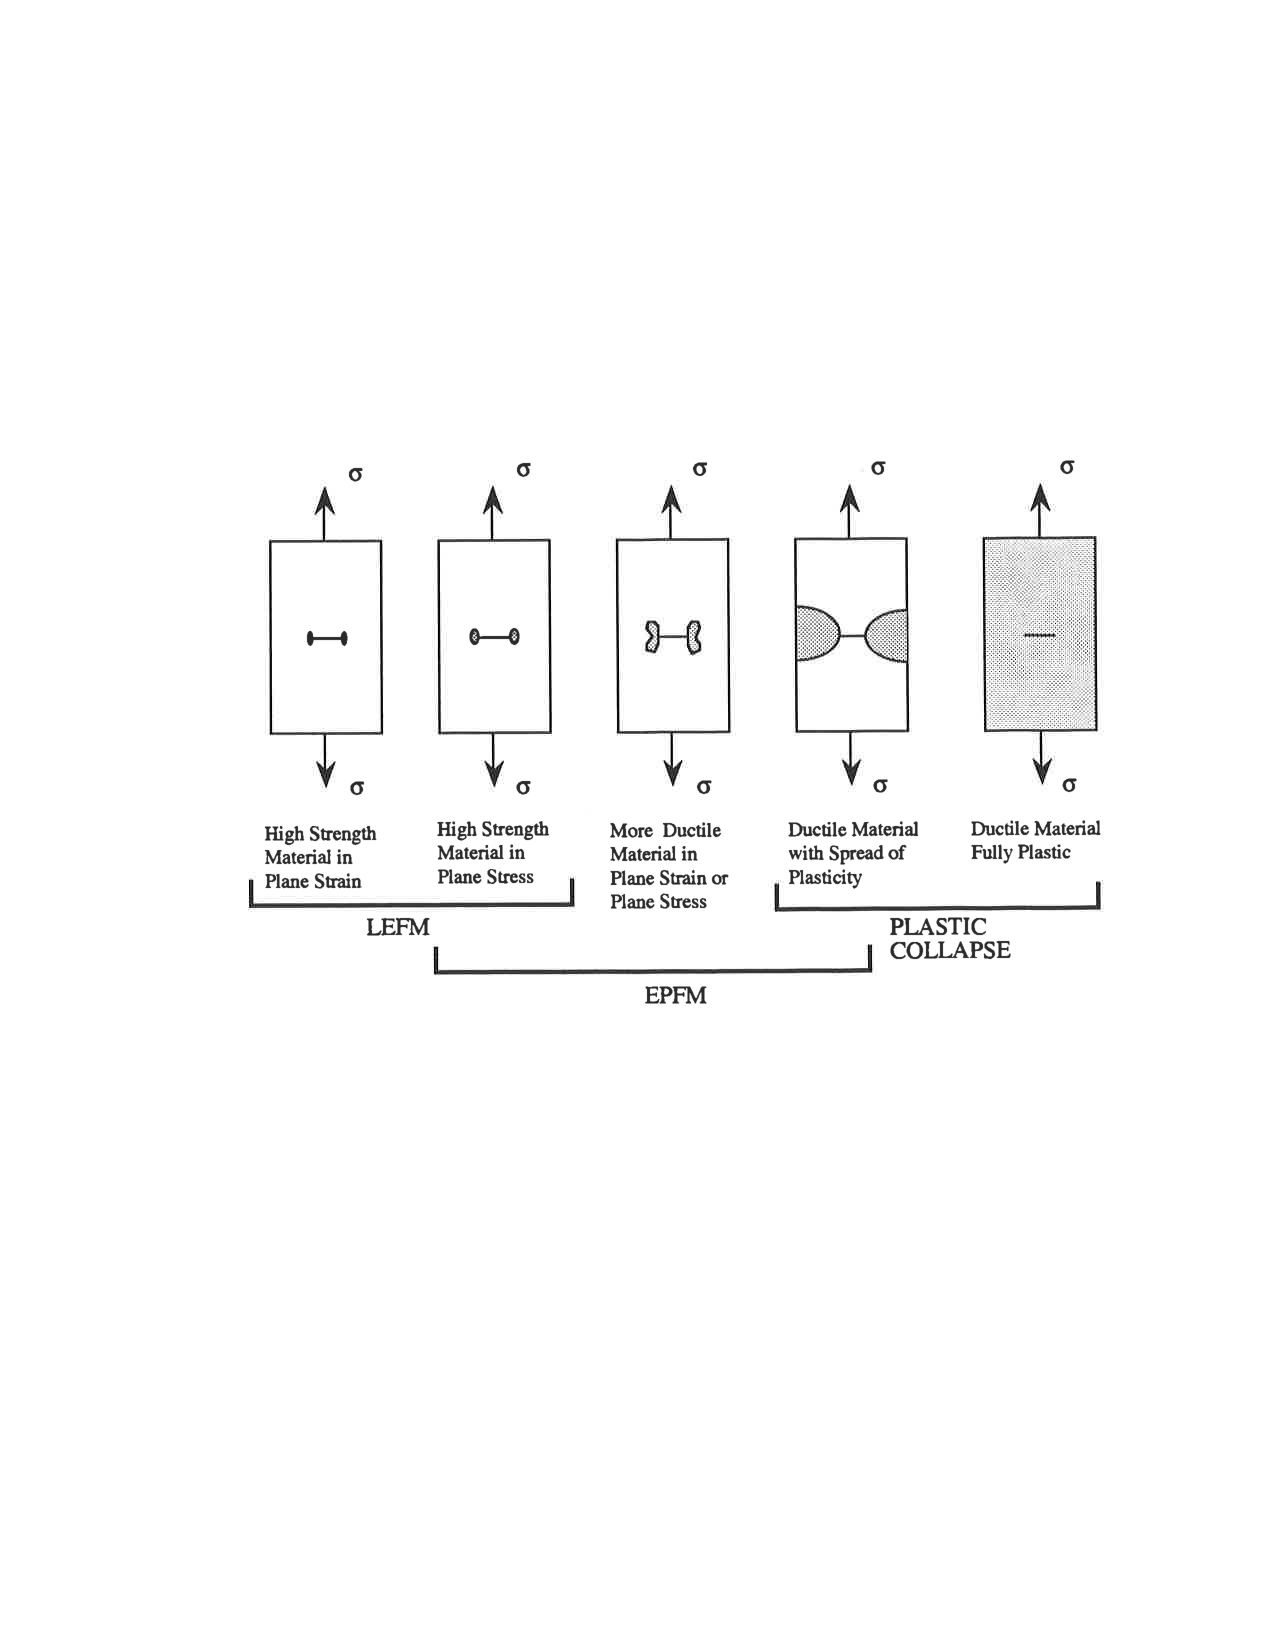
\includegraphics[width=0.7\columnwidth]{lefm-epfm-fp}
\caption[Categories of Fracture Mechanics Behaviors]{\label{fig:lefm-epfm-fp} Categories of Fracture Mechanics Behaviors \cite{janssenzuidemawanhill2002}}
\end{figure}

One of the significant challenges is to experimentally determine fracture toughness under elastic-plastic conditions.
This challenge is compounded by curved crack fronts, such as a surface crack in a plate subjected to tension or bending.
While test standards such as ASTM E399 ``Standard Test Method for Linear-Elastic Plane-Strain Fracture Toughness \KIc of Metallic Materials''~\cite{astme399} and ASTM E1820 ``Standard Test Method for Measurement of Fracture Toughness''~\cite{astme1820} are used for test specimen geometries with through cracks (a crack that goes completely through the cross section), test specimen geometries with surface cracks require an additional level of complexity.
ASTM E740 ``Standard Practice for Fracture Testing with Surface-Crack Tension Specimens''~\cite{astme740} addresses surface cracks, but only for linear elastic materials.
ASTM E399, ASTM E740, and ASTM E1820 have all reached a level of maturity and use but none address surface crack geometries for elastic-plastic materials.
ASTM E2899\footnote{As of November 2018, the current revision of ASTM E2899 was \href{https://www.astm.org/Standards/E2899.htm}{E2899-15}.} ``Standard Test Method for Measurement of Initiation Toughness in Surface Cracks Under Tension and Bending''~\cite{astme2899} was developed specifically to address surface crack geometries in tension and bending for elastic-plastic materials.
A supporting analysis tool for tension has been developed by Allen of NASA~\cite{allenwells2014}.
However, the tool does not include the supporting analysis to easily perform measurement of fracture toughness in bending.

The motivation of this research is to address the shortcomings of ASTM E2899 with regard to fracture toughness of surface cracks in flat plates subjected to bending.
In doing so, the current research must closely follow established techniques in verification and validation to ensure accurate results suitable for a range of crack shape geometries and elastic-plastic materials.
The primary goal of this research is to extend the existing tool to support bending conditions.

\section{Surface Cracks}

Surface cracks such as the one shown in \Cref{fig:sc-terminology-e2899} are some of the most common discontinuities found in structural components, and can be caused by scratches, surface finish quality, tool strikes, welding procedures, and other phenomena.
\begin{figure}[tbp]
\centering
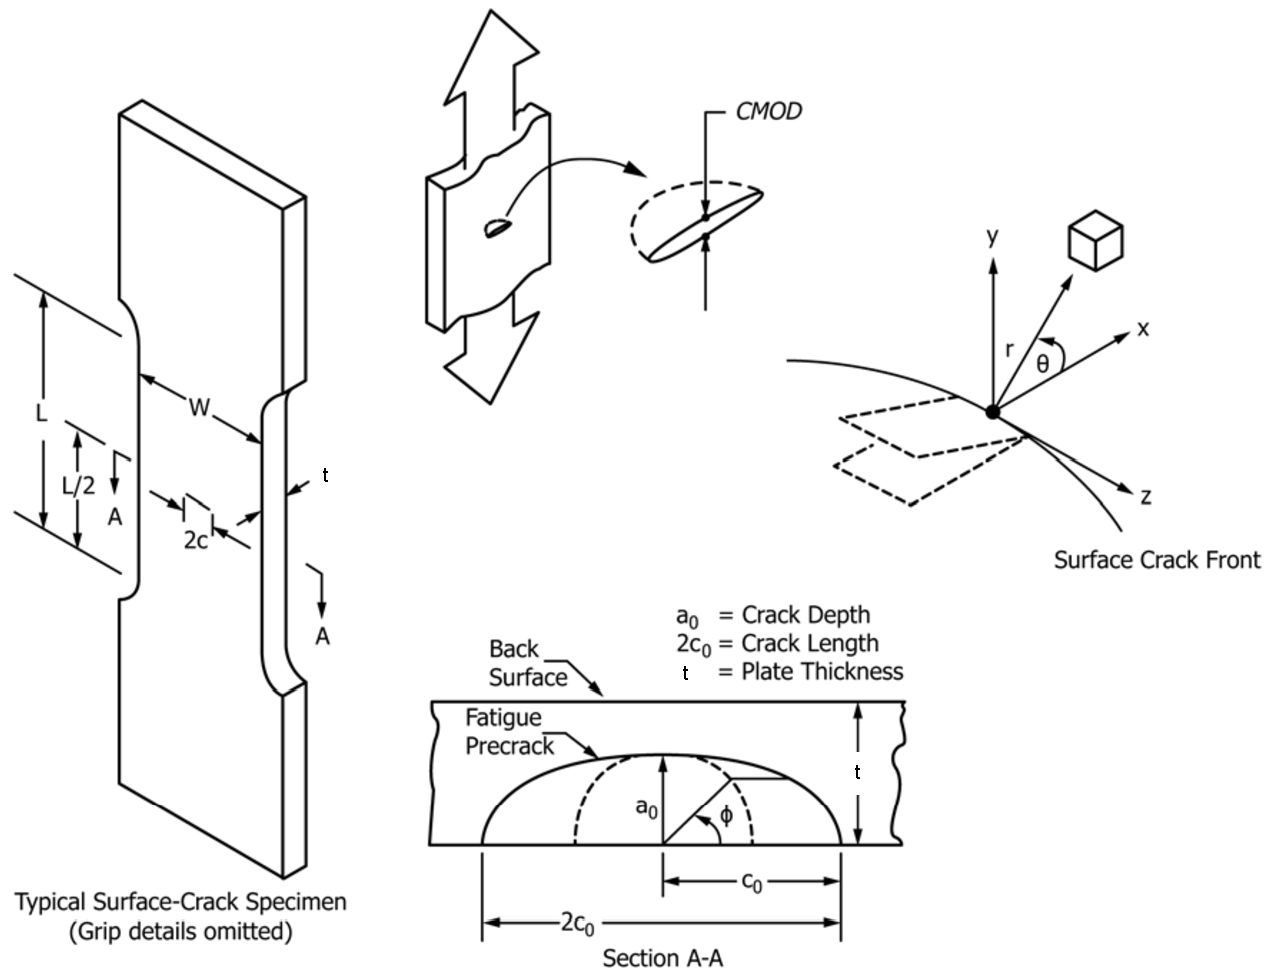
\includegraphics[width=0.95\columnwidth]{sc-terminology-e2899-modified}
\caption[ASTM E2899 Test Specimen and Crack Configurations]{\label{fig:sc-terminology-e2899} ASTM E2899 Test Specimen and Crack Configurations \cite{astme2899}}
\end{figure}
Surface crack geometry is inherently three-dimensional and the stress states around the perimeter of the crack can vary from a practically plane-stress state on the free surface to a practically plane-strain state at the deepest part of the crack.
Computationally, the modeling of stress state and fracture criteria around the perimeter of a surface crack requires a fine level of discretization not required for two-dimensional edge cracks or center cracks.

Surface cracks (especially surface cracks in bending) are subject to a wide range of local stress conditions beyond the plane-stress/plane-strain distinction.
These localized conditions are defined as constraint, and affect the influence of the Poisson effect on deformation and strain.
Where constraint levels are high, a hydrostatic stress state exists that allows higher stresses to develop without a corresponding amount of localized yielding or plastic deformation.
The constraint may lead to lower measurements of fracture toughness compared to an otherwise identical region of material subject to less constraint.
In regions with high constraint, the linear elastic stress intensity \K or the elastic-plastic strain energy release rate \J accurately predicts crack growth or failure, and the exact level of constraint has little effect on toughness measurements.
In regions with low constraint, \K or \J is coupled with a constraint measure (\(Q\), \(\Omega\), or a normalized Williams \(T\) stress) to predict crack growth or failure, as seen in \Cref{fig:toughness-constraint-locus}.
\begin{figure}[tbp]
\centering
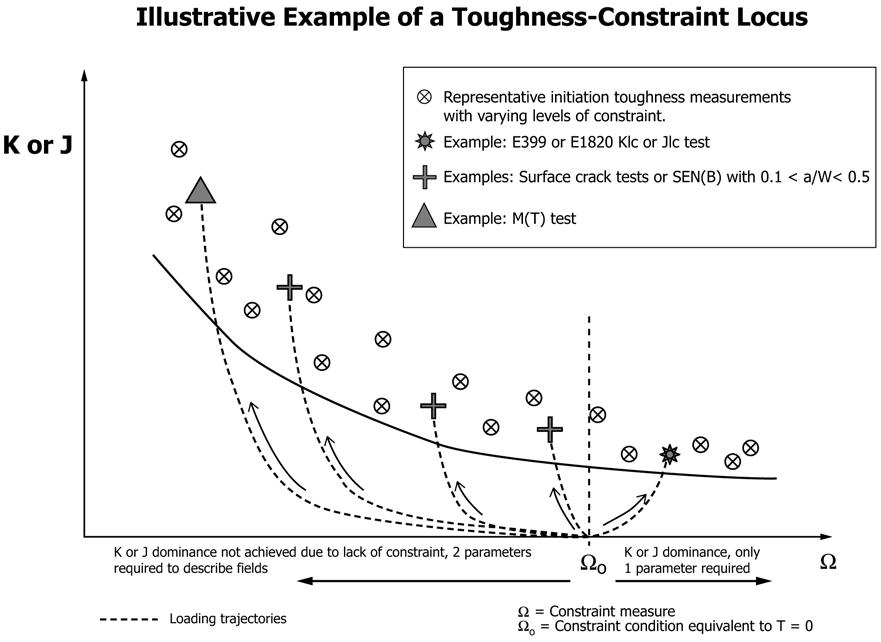
\includegraphics[width=0.9\columnwidth]{toughness-constraint-locus}
\caption[Example of Toughness-Constraint Locus]{\label{fig:toughness-constraint-locus} Example of Toughness-Constraint Locus \cite{astme2899}}
\end{figure}

The semi-elliptical surface crack in a flat plate is one of the simpler types of part-through cracks, and \Cref{fig:nasgro-geometries} show other types of surface cracks, including those at corners, in spheres, or in solid or hollow cylinders.
Handbook or other curve-fitted solutions exist for all these geometries, but only for linear elastic materials.
Regardless of the specific geometry, all these geometries exhibit varying levels of constraint around the crack front, and no simple solutions exist for characterizing their elastic-plastic fracture properties.
\begin{figure}[tbp]
\centering
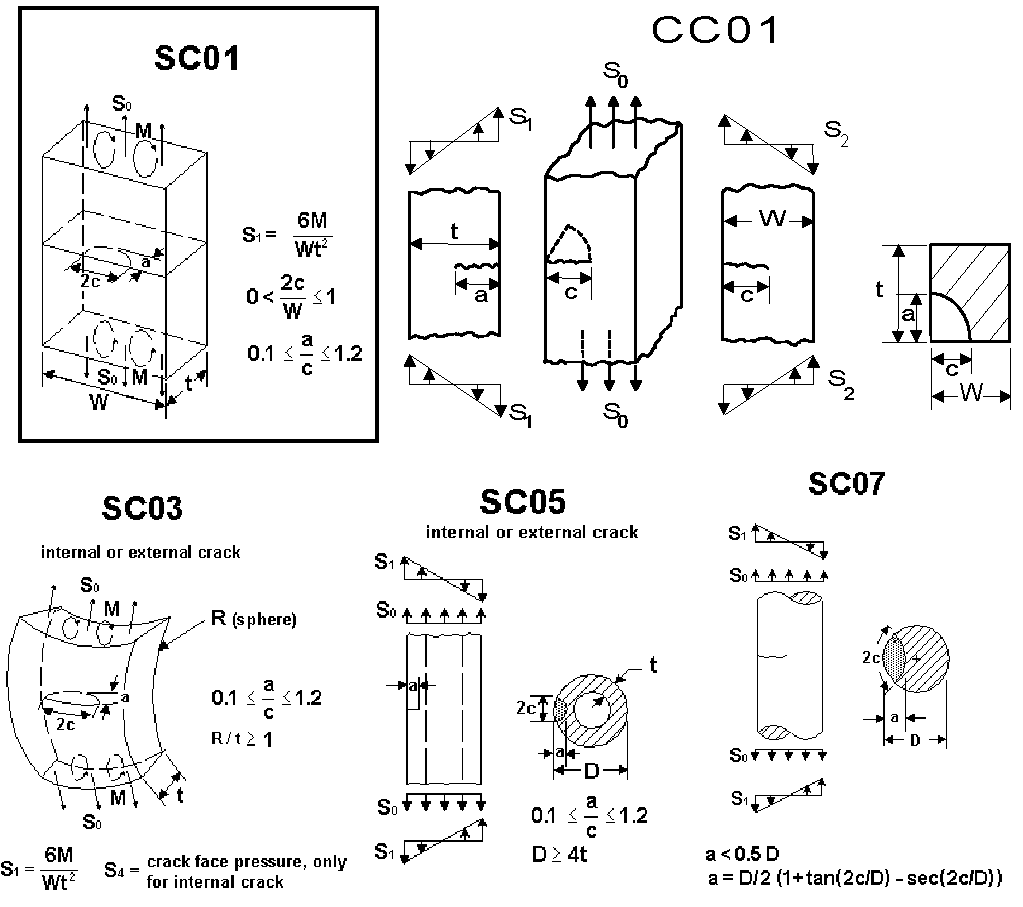
\includegraphics[width=0.8\columnwidth]{nasgro-geometries}
\caption[NASGRO Surface Crack Geometries]{\label{fig:nasgro-geometries} NASGRO Surface Crack Geometries \cite{nasgro2000}}
\end{figure}

\section{Mechanical Properties and Fracture Toughness Standards}

Several standards for evaluating mechanical properties, including fracture toughness, have been developed by ASTM International and other standards bodies.
These standards are predominantly experimental, with limited calculations and analysis required.
Both ASTM E8, ``Standard Test Methods for Tension Testing of Metallic Materials,''~\cite{astme8} ASTM E399, ``Standard Test Method for Linear-Elastic Plane-Strain Fracture Toughness \KIc of Metallic Materials,''~\cite{astme399}, and ASTM E740, ``Standard Practice for Fracture Testing with Surface-Crack Tension Specimens,''~\cite{astme740} all use linear curve fits and basic calculations that could be completed with a strip chart and a calculator.
ASTM E1820, ``Standard Test Method for Measurement of Fracture Toughness,''~\cite{astme1820} uses a series of equations to calculate \K and an elastic component of \J, and calculates a plastic component of \J from the area under a load-displacement curve. These calculations could be completed with a spreadsheet.
ASTM E2899 details methods for measuring fracture toughness in flat specimens like those shown in \Cref{fig:sc-terminology-e2899}.
ASTM E2899 is a major departure from earlier standards in that it requires an elastic-plastic finite element analysis to calculate required \J values.
In 2014, one year after the initial release of ASTM E2899, Phillip Allen of NASA Marshall Space Flight Center released the Tool for the Analysis of Surface Cracks program (TASC) to help meet the analysis requirements of the standard.
TASC uses a database of finite element results for 600 surface-cracked plates covering a wide range of crack geometries and plate material properties, and interpolates results for intermediate geometries and material properties from the database.
This reduces the difficulty of complying with ASTM E2899, but the 2014 TASC program only applies to flat plates in tension, not in bending.

\section{Research Goals}
\label{sec:research-goals}

As of 2018, fracture toughness of a body with a surface crack can be readily evaluated for linear elastic materials in tension or bending by using handbook equations, or for elastic-plastic materials in tension by using TASC.
No such method exists for elastic-plastic materials in bending, so the primary goal of this research will be to create a database equivalent to the TASC tension database, and to modify the existing TASC program to support bending experiments.
To help ensure high quality results, a literature review in \Cref{chap:literature-review} includes consensus solutions for calculation of stress intensity factors, numerical methods for elastic-plastic and fully-plastic fracture mechanics of plates in bending, and techniques for verification and validation of results.
A short verification of tensile surface crack problems in \Cref{sec:verification-tasc} demonstrates techniques used to develop the bending model database.
The development of the bending database is detailed in \Cref{chap:research-plan}, including defining the plate models in terms of a few fundamental parameters, modifying boundary conditions to reach sufficient levels of elastic-plastic behavior, and extracting and compiling necessary results from the simulations into a the final database and modified version of TASC.
A set of force versus crack mouth opening displacement (CMOD)\nomenclature[1CMOD]{CMOD}{crack mouth opening displacement} data from a NASA tensile test is shown in \Cref{fig:force-cmod-phase-1}, and was used to judge finite element results from a variety of laboratories as part of a round-robin survey of surface crack modeling techniques shown in \Cref{fig:force-cmod-models-phase-1} \citep{wells2012analytical}.
Comparable data from a NASA bend test \cite{allen2018} is given in \Cref{fig:nasa-bend-p-cmod}, and it was used as a validation case in \Cref{chap:results}.
\begin{sidewaysfigure}
\centering
\begin{minipage}[b]{0.45\textwidth}
\centering
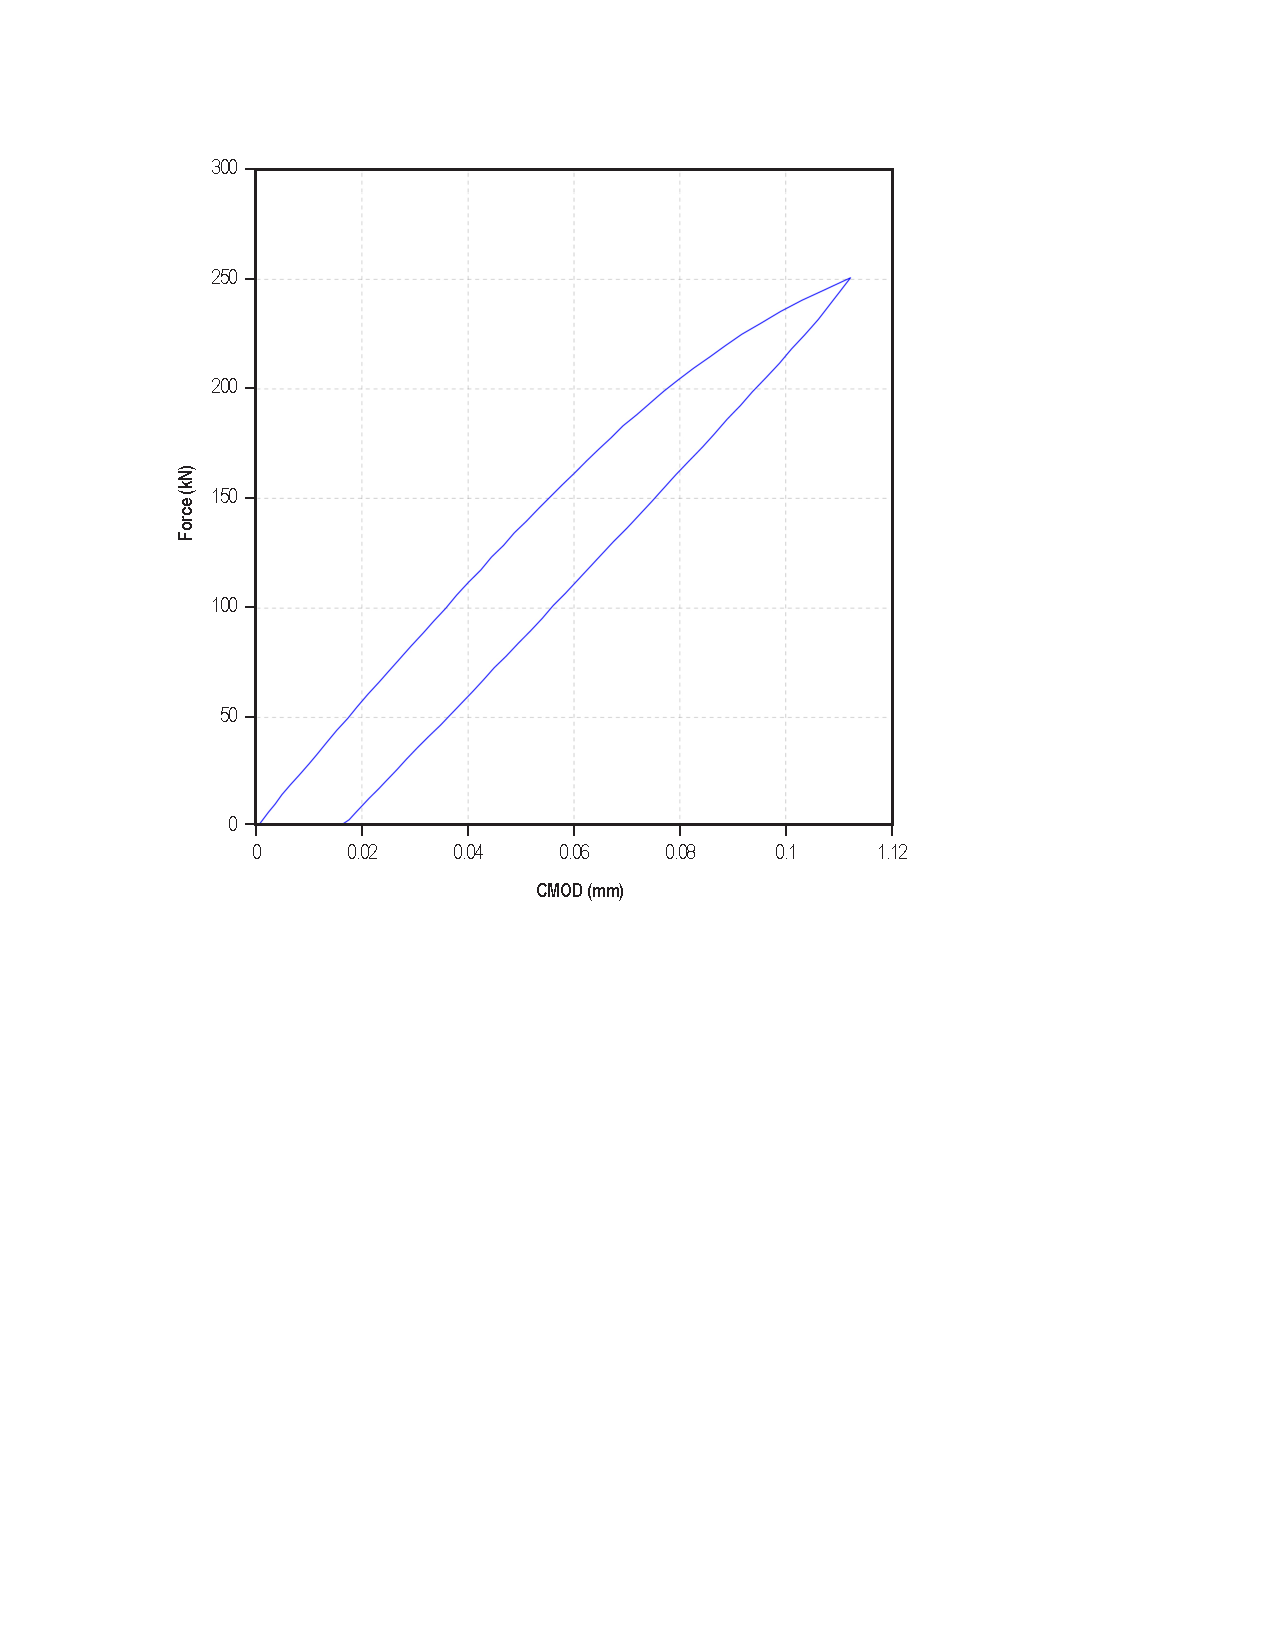
\includegraphics[height=3.64in]{force-cmod-phase-1}
\subcaption{\label{fig:force-cmod-phase-1} Tensile test}
\end{minipage}%
\begin{minipage}[b]{0.55\textwidth}
\centering
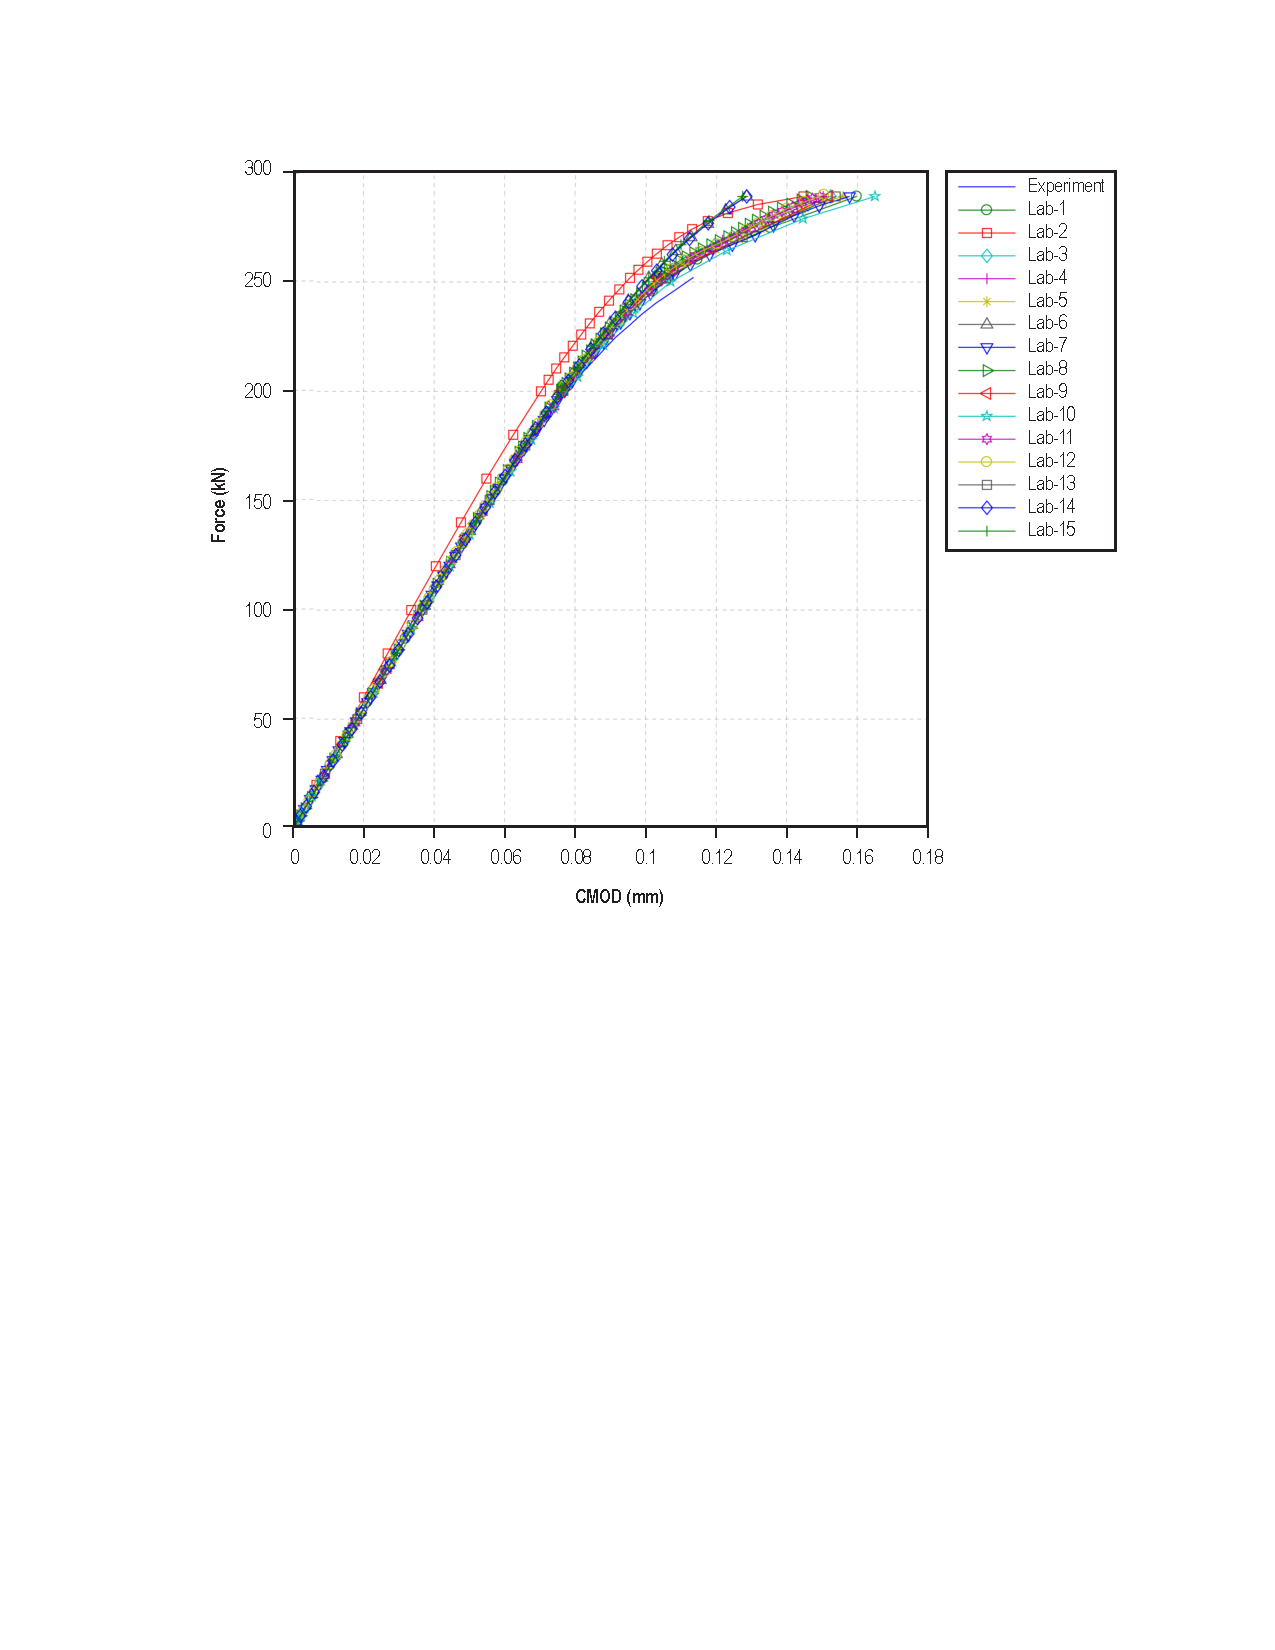
\includegraphics[height=3.64in]{force-cmod-models-phase-1}
\subcaption{\label{fig:force-cmod-models-phase-1} Comparison of finite element results to tensile test}
\end{minipage}
\caption[Force versus CMOD data from NASA experiment and round-robin finite element results]{Force versus CMOD data from NASA experiment and round-robin finite element results \citep{wells2012analytical}}
\end{sidewaysfigure}
\begin{figure}
\centering
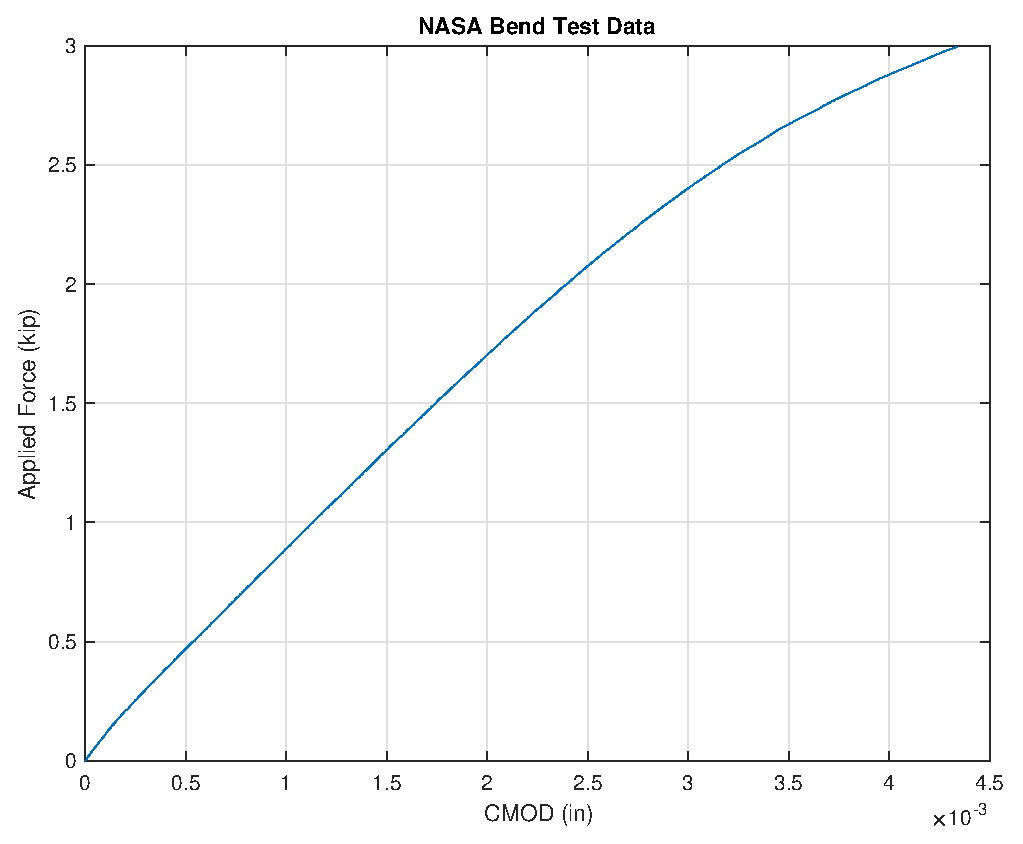
\includegraphics[width=\columnwidth]{nasa_bend_p_cmod}
\caption{\label{fig:nasa-bend-p-cmod} Force versus CMOD data from NASA bend test}
\end{figure}

The second goal of this research is an investigation of the applicability of estimating the elastic-plastic \J by summing elastic and fully-plastic \J values originally developed by the Electric Power Research Institute (EPRI)\nomenclature[1E]{EPRI}{Electric Power Research Institute}.
\Cref{sec:estimation} gives an overview of the EPRI estimation scheme,
\Cref{sec:h1-verification} summarizes some early work done with the EPRI technique for surface cracks in tension,
\Cref{chap:h1} briefly outlines plans for further verifications of the EPRI method,
and
\Cref{sec:epri-results} shows the results of the study.

The final goal of this research is an investigation of the applicability of the load separation technique~\citep{sharobeamlandes1991} to surface cracks in bending.
The load separation technique is a method analogous to separation of variables where the geometry-specific factors affecting \J are separated from the material-specific parameters affecting \J.
As seen in \Cref{fig:loadsep}, it results in a single-specimen technique that predicts behavior of a range of crack geometries for a given material.
Load separation was originally an experimental technique, but may also be applied to numerical models.
\begin{figure}[tbp]
\centering%
\begin{minipage}[t]{0.45\columnwidth}%
\centering%
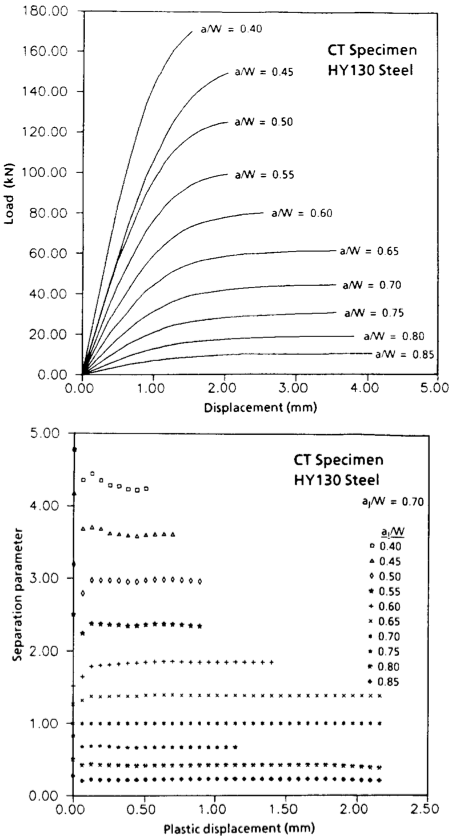
\includegraphics[width=\columnwidth]{load-sep-final}
\subcaption{Separation parameters}%
\end{minipage}%
\begin{minipage}[t]{0.45\columnwidth}%
\centering%
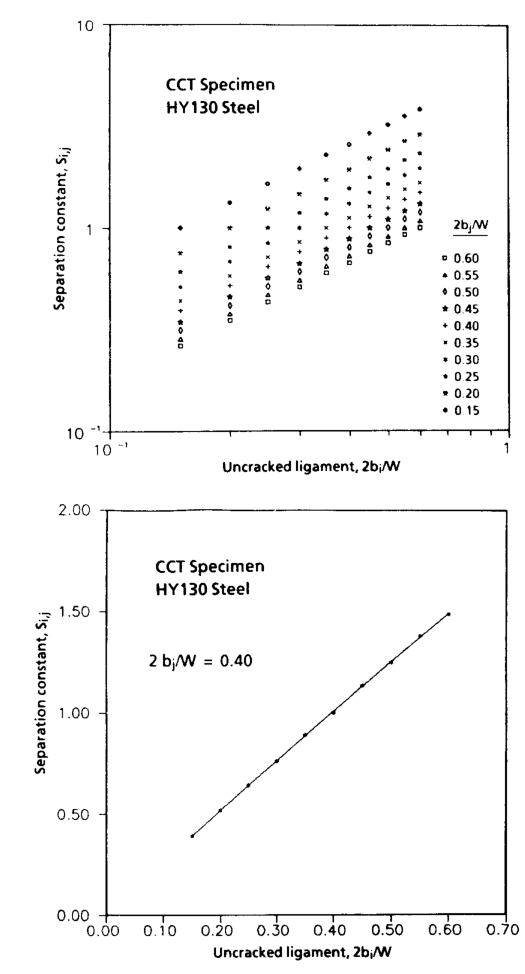
\includegraphics[width=\columnwidth]{load-separation-uncracked-ligament}%
\subcaption{Key curve for single-specimen technique}%
\end{minipage}%
\caption[Load separation technique]{\label{fig:loadsep} Load separation technique \citep{sharobeamlandes1991}}%
\end{figure}
An introduction to load separation is given in \Cref{sec:intro-load-separation}, 
the results of \citeauthor{sharobeamlandes1993}' study of surface cracks in tension \cite{sharobeamlandes1993} are replicated in \Cref{sec:loadsepverification},
\Cref{chap:load-separation} presents the plan for a more extensive study of load separation for surface cracks in bending,
and
\Cref{sec:results-loadsep} shows the results of the bending study.

\chapter{Literature Review}
\label{chap:literature-review}

This chapter will detail the consensus solution for linear elastic stress intensity factors, historical development of failure assessment standards, limits of single-parameter fracture, and estimation techniques for elastic-plastic fracture parameters\footnote{\Cref{chap:app-intro-fracture} provides an overview of the basis of linear elastic fracture mechanics and elastic-plastic fracture mechanics.}.
Finally, this chapter will review ASTM E2899, related tools for analysis of surface cracks in tension, and techniques to ensure accurate and reliable results for analysis of surface cracks in bending.
These are three key components that will be expanded upon in this research.

\section{Consensus Bending Stress Intensity Factor Solution}

A consensus solution for linear elastic stress intensity factors in tension or bending was achieved after many years of discussion and debate.
For example, the Society for Experimental Stress Analysis~\cite{sesa1980} reviewed a range of both numerical and experimental methods for calculating or measuring stress intensity and summarized the relative accuracy and deficiencies in the methods.
Examples of the range of stress intensity solutions are given in \Cref{fig:prior_research_1,fig:prior_research}.
Scott and Thorpe~\cite{scottthorpe1981} reviewed several numerical methods for calculating stress intensity, and identified where the methods diverged substantially.
ASTM E2899 provides a general equation for calculating the linear elastic stress intensity factor \KI for combined tension and bending loading at any position \(\phi\) along the crack front, first published by Newman, Raju, et al. \cite{newmanraju1983a,newmanreuter2000}.
In the absence of applied tension, these equations can be simplified to \Crefrange{eq:e2899-ki}{eq:e2899-g2}.
\begingroup
\allowdisplaybreaks
\begin{align}
\KI &= (
        H \sigma_\text{b} F_\text{b}
        ) \left(\frac{\pi a}{Z}\right)^{0.5} \label{eq:e2899-ki} \\
\sigma_\text{b} &= \frac{6 M}{W t^2} \\
Z &= 1 + 1.464\left(\frac{a}{c}\right)^{1.65} \\
F_\text{b} &= \left[ M_1 + M_2 \left( \frac{a}{t} \right)^2 + M_3 \left( \frac{a}{t} \right)^4 \right] f_\phi f_\text{wb} g \\
M_1 &= 1.13 - 0.09 \left( \frac{a}{c} \right) \\
M_2 &= -0.54 + \left( \frac{0.89}{0.2 + \frac{a}{c}} \right) \\
M_3 &= 0.5 - \frac{1.0}{0.65+\frac{a}{c}} + 14\left( 1.0 - \frac{a}{c} \right)^{24} \\
f_\phi &= \left[ \left( \frac{a}{c} \right)^2 \cos^2 \phi + \sin^2 \phi \right]^{0.25} \\
f_\text{wb} &= \left\{ \sec \left[ \left( \frac{\pi c}{W} \right) \left( \frac{a}{t} \right)^{0.5} \right] \right\}^{0.5} \\
g &= 1+ \left[ 0.1 + 0.35 \left( \frac{a}{t} \right)^2 \right] (1 - \sin \phi)^2 \\
H &= H_1 + (H_2 - H_1) (\sin \phi)^p \\
p &= 0.2 + \frac{a}{c} + 0.6 \left( \frac{a}{t} \right) \\
H_1 &= 1 - 0.34 \left( \frac{a}{t} \right) - 0.11 \frac{a}{c} \left( \frac{a}{t} \right) \\
H_2 &= 1 + G_1 \left( \frac{a}{t} \right) + G_2 \left( \frac{a}{t} \right)^2 \\
G_1 &= -1.22 - 0.12 \left( \frac{a}{c} \right) \\
G_2 &= 0.55 - 1.05 \left( \frac{a}{c} \right)^{0.75} + 0.47 \left( \frac{a}{c} \right)^{1.5} \label{eq:e2899-g2}
\end{align}
\endgroup
These equations are derived from curve fits to finite element results, and popular fracture mechanics software including NASGRO and AFGROW use this consensus solution as the basis for their stress intensity calculations, but no comparable equation exists for the elastic-plastic fracture parameter \J.

\section{Failure Assessment Diagrams and Fitness for Purpose Standards}

Through the 1960s, structural discontinuities including porosity and weld slag inclusion were identified with non-destructive testing (NDT)\nomenclature[1N]{NDT}{Non-destructive testing} and classified by volumetric size \citep{WIESNER2000883}.
These methods could easily overlook planar discontinuities such as cracks, and the repairs required to correct the larger volumetric discontinuities could introduce additional planar discontinuities,
reducing the overall structural quality.
Fitness for purpose (FFP)\nomenclature[1F]{FFP}{fitness for purpose} standards were created to evaluate discontinuities
in terms of their impact on all aspects of structural integrity.
Prominent FFP standards include the R6 standard \citep{r6-1976} and PD~6493 \citep{pd6493-1991} which was later revised as BS~7910 \citep{bs7910-1999}.
Commonly used in FFP standards, the failure assessment diagram (FAD)\nomenclature[1F]{FAD}{failure assessment diagram} is a method of evaluating if a body will be able to withstand certain applied conditions without failing.
It can be considered an extension of simpler evaluation methods such as a factor of safety against yielding, and is similar to a stress-life or strain-life curve when designing for fatigue.

On a simpler factor of safety calculation, the applied conditions determine a stress state and stress magnitude (maximum normal stress, maximum shear stress, von Mises stress, etc.).
If the stress magnitude exceeds a criteria specific to the material (typically a yield stress), the body is considered to have failed and must be redesigned.
On a stress-life evaluation, the applied conditions determine a stress magnitude, and if the number of cycles required at this magnitude exceeds an experimentally-determined material life for this stress level (a point falling outside the region bounded by the stress-life curve), the body is considered to have failed.

\subsection{Failure Assessment Diagrams for Linear Elastic Behavior}

A typical FAD including fracture criteria (\K or \J) will require calculating a stress criterion from the net section stress near a crack, and calculating a fracture criterion from an appropriate stress intensity or strain energy.
A simple FAD for a cracked body made from a brittle material with purely elastic behavior would require net section stress values to remain below the ultimate strength of the material, and \K values at the crack tip to remain below the critical \KIc value associated with brittle failure.
These criteria are assumed to be independent of each other (as \K is proportional to both crack length and applied stress), resulting in a rectangular region on the FAD signifying conditions where the body does not experience failure shown in \Cref{fig:brittle-fad}.
\begin{figure}
\centering
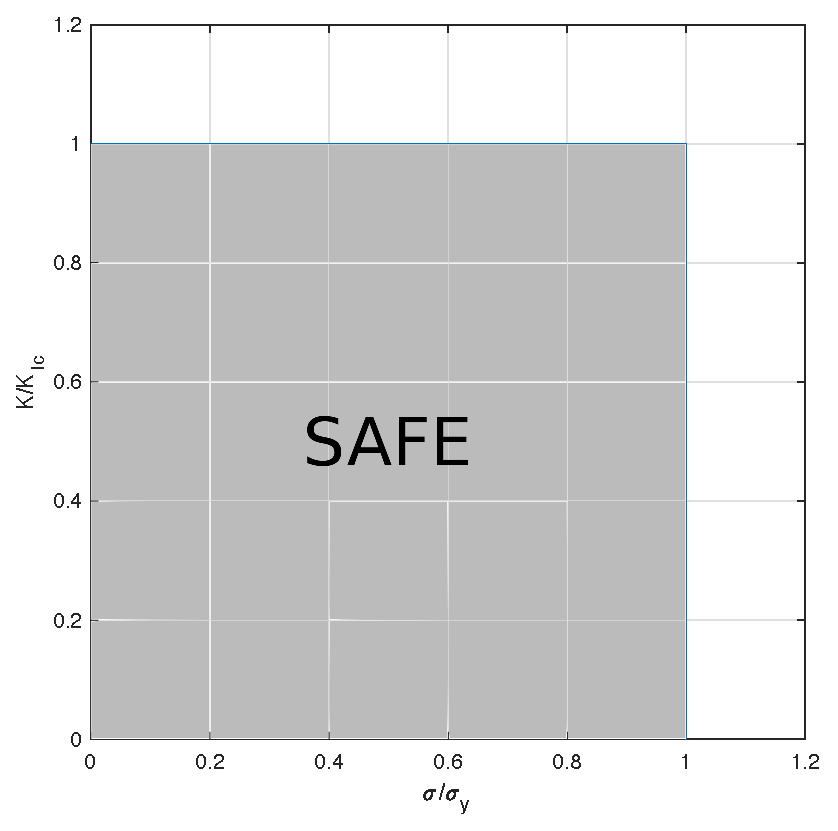
\includegraphics[width=0.6\columnwidth]{brittle-fad-modified}
\caption{\label{fig:brittle-fad} Failure assessment diagram for brittle material}
\end{figure}
Points outside the rectangular region indicate structural failure, either due to fracture or excessive yielding.

\subsection{Failure Assessment Diagrams for Plastic Behavior}

Materials that exhibit some plastic behavior can be stressed beyond their elastic limit, and their locus of failure will be more complicated than a simple rectangle.
A plastic collapse condition, where stress in the body causes plastic hinges to form and the structure becomes geometrically unstable, may be substituted for ultimate strength.
\citet{dowling1975} and Harrison et al. \cite{r6-1976} applied a strip yield model to create one of the first elastic-plastic FADs in the British Central Electricity Generating Board's R6 report.
The effective (plasticity-corrected) stress intensity at the crack tip using a strip yield model is
\begin{align}
\Kef &= \Sy \sqrt{\pi a} \left[ \frac{8}{\pi^2} \ln \sec \frac{\pi \sigma}{2 \Sy} \right]^{\frac{1}{2}}.
\end{align}
The strip yield model is used to account for the effect of the plastic zone on the stress intensity factor \KI.
If the plastic collapse stress \Sc is substituted in place of the yield strength \Sy, this becomes
\begin{align}
\Kef &= \Sc \sqrt{\pi a} \left[ \frac{8}{\pi^2} \ln \sec \frac{\pi \sigma}{2 \Sc} \right]^{\frac{1}{2}}.
\end{align}
Here, the plastic collapse stress is often taken as the average of the material's yield strength \Sy and its ultimate strength \Sut.
If the effective stress intensity is divided by the linear elastic stress intensity factor
\begin{align}
\KI &= \sigma \sqrt{\pi a},
\end{align}
this results in a dimensionless stress intensity ratio
\begin{align}
\frac{\Kef}{\KI} &= \frac{\Sc}{\sigma} \left[ \frac{8}{\pi^2} \ln \sec \frac{\pi \sigma}{2 \Sc} \right]^{\frac{1}{2}}
\end{align}
which can be rewritten in terms of a \K ratio \(\Kr=\frac{\Kef}{\KI}\) and stress ratio \(\Sr = \frac{\sigma}{\Sc} \) as
\begin{align}
\Kr &= \Sr  \left[ \frac{8}{\pi^2} \ln \sec \frac{\pi}{2} \Sr \right]^{\frac{1}{2}},
\end{align}
resulting in a FAD on a normalized scale shown in \Cref{fig:strip-yield-fad}, the R6 curve.
\begin{figure}
\centering
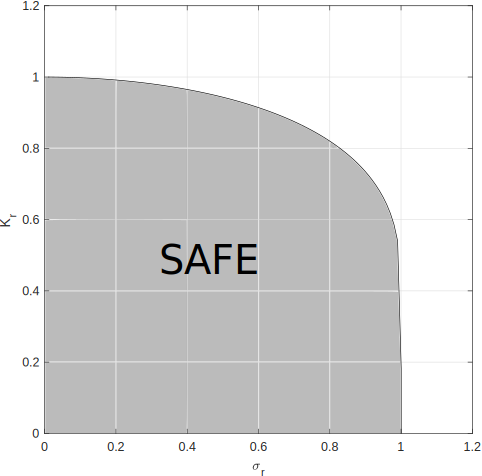
\includegraphics[width=0.6\columnwidth]{strip-yield-fad-modified}
\caption{\label{fig:strip-yield-fad} Failure assessment diagram using strip yield model (R6 curve)}
\end{figure}
Similar to the simpler FAD of \Cref{fig:brittle-fad}, points outside the curve indicate structural failure, whether due mostly to fracture (where \Sr is small, but \Kr is large), mostly to plastic collapse (\(\Sr > 1\)), or a combination of both (e.g., \(\Kr = \Sr = 0.85\)).

If loading paths are added to \Cref{fig:strip-yield-fad}, the resulting graph can show how stable crack growth alters the FFP assessment.
A load path for a stable crack of size \(\frac{a}{W}=0.2\) under monotonically increasing load is shown as the dashed line in \Cref{fig:strip-yield-fad-extra}.
As both \Kr and \Sr are proportional to the applied stress, this is a straight line.
The factor of safety for a load applied to a given crack size is calculated by the ratio of the length of a straight line from the origin to its intersection with the R6 curve versus the length of a straight line segment from the origin to its intersection with a load curve---approximately 2.5 when \(\Sr = 0.25\), or 1.0 when \(\Sr = 0.61\).
\begin{figure}
\centering
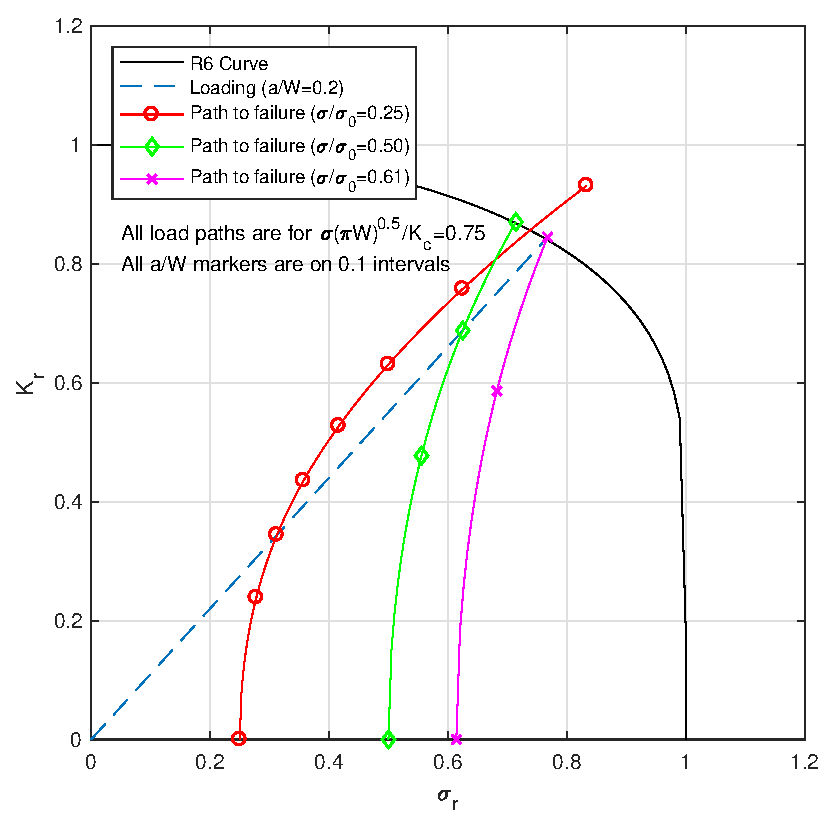
\includegraphics[width=0.6\columnwidth]{strip-yield-fad-extra}
\caption{\label{fig:strip-yield-fad-extra} Failure assessment diagram using strip yield model, including paths to failure}
\end{figure}
\begin{figure}
\centering
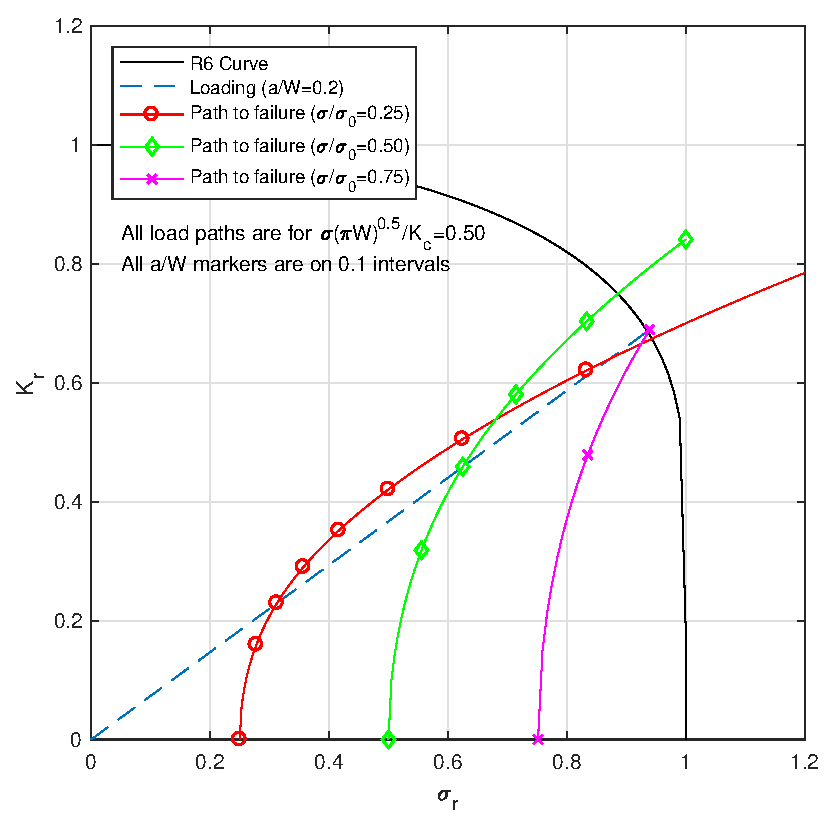
\includegraphics[width=0.6\columnwidth]{strip-yield-fad-extra-2}
\caption{\label{fig:strip-yield-fad-extra-2} Failure assessment diagram of material with higher fracture toughness using strip yield model}
\end{figure}
\begin{figure}
\centering
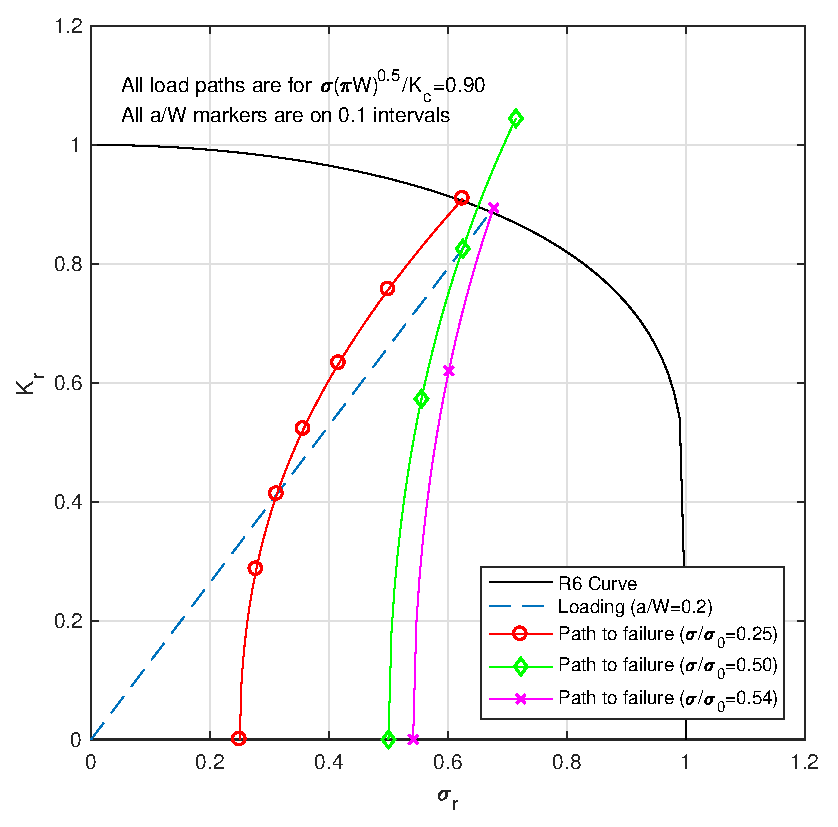
\includegraphics[width=0.6\columnwidth]{strip-yield-fad-extra-3}
\caption{\label{fig:strip-yield-fad-extra-3} Failure assessment diagram of material with lower fracture toughness using strip yield model}
\end{figure}
A material with identical strength but higher fracture toughness is shown in \Cref{fig:strip-yield-fad-extra-2} with the same crack size and initial applied loads.
As expected, the FAD indicates this material is more prone to plastic collapse failure than fracture.
At a given applied load, cracks grow to larger lengths before fracture, and additional load is required to fracture a specimen with a given crack length (\(\frac{\sigma}{\sigma_0} = 0.75\) for \(\frac{a}{W}=0.2\)).
A material with identical strength but lower fracture toughness is shown in \Cref{fig:strip-yield-fad-extra-3} with the same crack size and initial applied loads.
As expected, the FAD indicates this material is more prone to fracture than plastic collapse failure.
At a given applied load, cracks grow to shorter lengths before fracture, and less load is required to fracture a specimen with a given crack length (\(\frac{\sigma}{\sigma_0} = 0.54\) for \(\frac{a}{W}=0.2\)).

\subsection{Failure Assessment Diagrams for Elastic-Plastic Behavior}

Applying a strip-yield model to the failure assessment diagram leads to conservative estimates of failure, since it assumes plastic collapse when net section stresses reach \(\sigma_0\) \citep{kanninen1985}.
For materials that strain harden, the net section becomes stronger and can withstand stresses higher than \(\sigma_0\).
Failure assessment diagrams for elastic-plastic behavior will require both the non-linear stress intensity parameter \J and a strain-hardening material model, such as the Ramberg-Osgood power-law material model given in \Cref{fig:ramberg-osgood}.

The elastic-plastic FAD will depend on material strength, the hardening exponent \(n\), and strain energy in the form of the \J integral. As \J itself depends on specimen geometry and loading configuration, a single FAD curve becomes a family of curves.
\J can be expressed as the sum of an elastic component \Jel and a plastic component \Jpl, with the elastic and plastic components \Jel and \Jpl having the form of
\begin{align}
\Jel(\aapp) &= \tilde{J}_\textnormal{el}(\aapp) \left(\frac{P}{P_0}\right)^2 \\
\Jpl(a, n) &= \tilde{J}_\textnormal{pl}(a, n) \left(\frac{P}{P_0}\right)^{(n+1)}.
\end{align}
At fracture, \(\J = \J_\textnormal{c} = \Jel(\aapp) + \Jpl(a,n)\), and an equivalent to \Kr can be written as

\begin{align}
\J_\textnormal{r} = \frac{\Jel(a)}{\J_\textnormal{c}} &= \frac{\tilde{J}_\textnormal{el}(a) \left(\frac{P}{P_0}\right)^2}{\tilde{J}_\textnormal{el}(\aapp) \left(\frac{P}{P_0}\right)^2 + \tilde{J}_\textnormal{pl}(a, n) \left(\frac{P}{P_0}\right)^{(n+1)}} \nonumber \\
&= \frac{\tilde{J}_\textnormal{el}(a)}{\tilde{J}_\textnormal{el}(\aapp) + \tilde{J}_\textnormal{pl}(a, n) \left(\frac{P}{P_0}\right)^{(n-1)}},
\end{align}
which follows the same trends as \Kr:
as the applied load \(P \rightarrow 0 \),
\( \J_\textnormal{r} \rightarrow \frac{\tilde{J}_\textnormal{el}(a)}{\tilde{J}_\textnormal{el}(\aapp)} = 1 \),
and as \(P \rightarrow \infty \),
\(\tilde{J}_\textnormal{pl} \gg \tilde{J}_\textnormal{el}\), \(\frac{P}{P_0} \rightarrow \infty \) and \(\J_\textnormal{r} \rightarrow 0 \).

The influence of the hardening exponent \(n\) on the FAD for a center-cracked panel in plane stress with \(\frac{a}{W} = 0.5\) is shown in \Cref{fig:fad-ccp-multiple-n} (with \(S_{\text{r}} = \Sr\)), where materials with increased stress hardening are more likely to fail in fracture than in exceeding material strength.
\begin{figure}
\centering
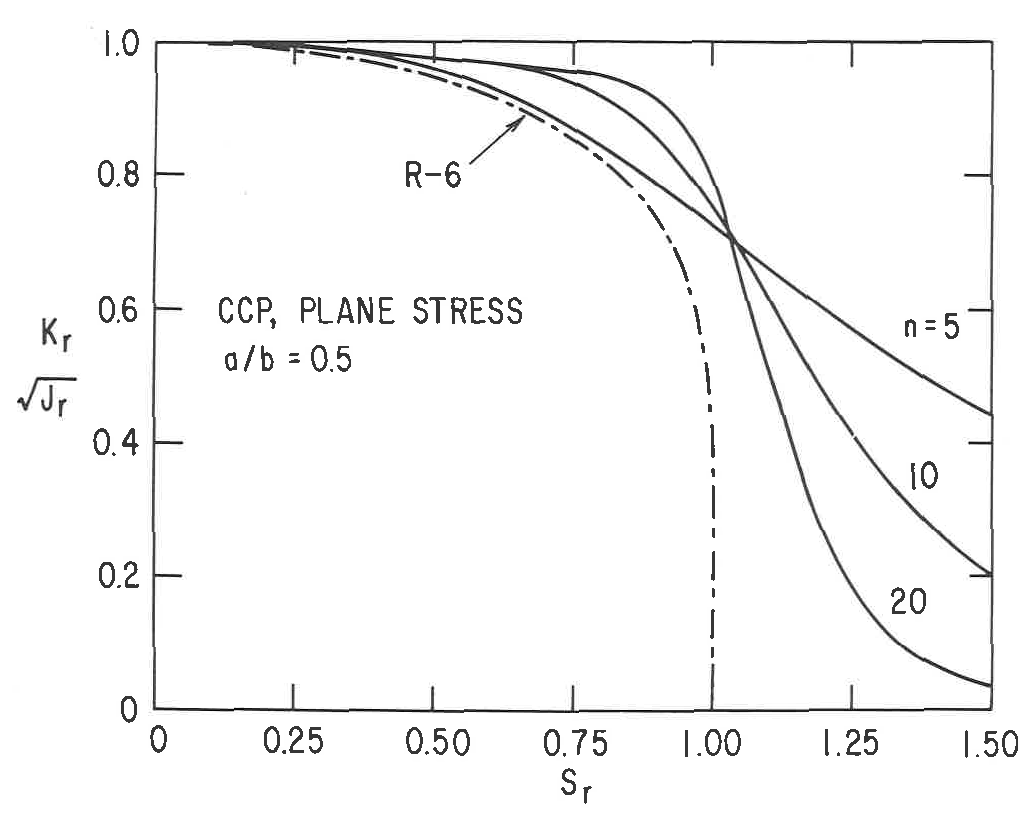
\includegraphics[width=0.7\columnwidth]{FAD-variance-n-modified}
\caption[Failure assessment diagram of center-cracked panel with multiple hardening exponents]{\label{fig:fad-ccp-multiple-n} Failure assessment diagram of center-cracked panel with multiple hardening exponents \cite{epri1981}}
\end{figure}
The influence of plane stress and plane strain conditions on the FAD for a center-cracked panel and a compact tension specimen with \(\frac{a}{W} = 0.5, n = 10\) is shown in \Cref{fig:fad-ccp-ct}.
\begin{figure}
\centering
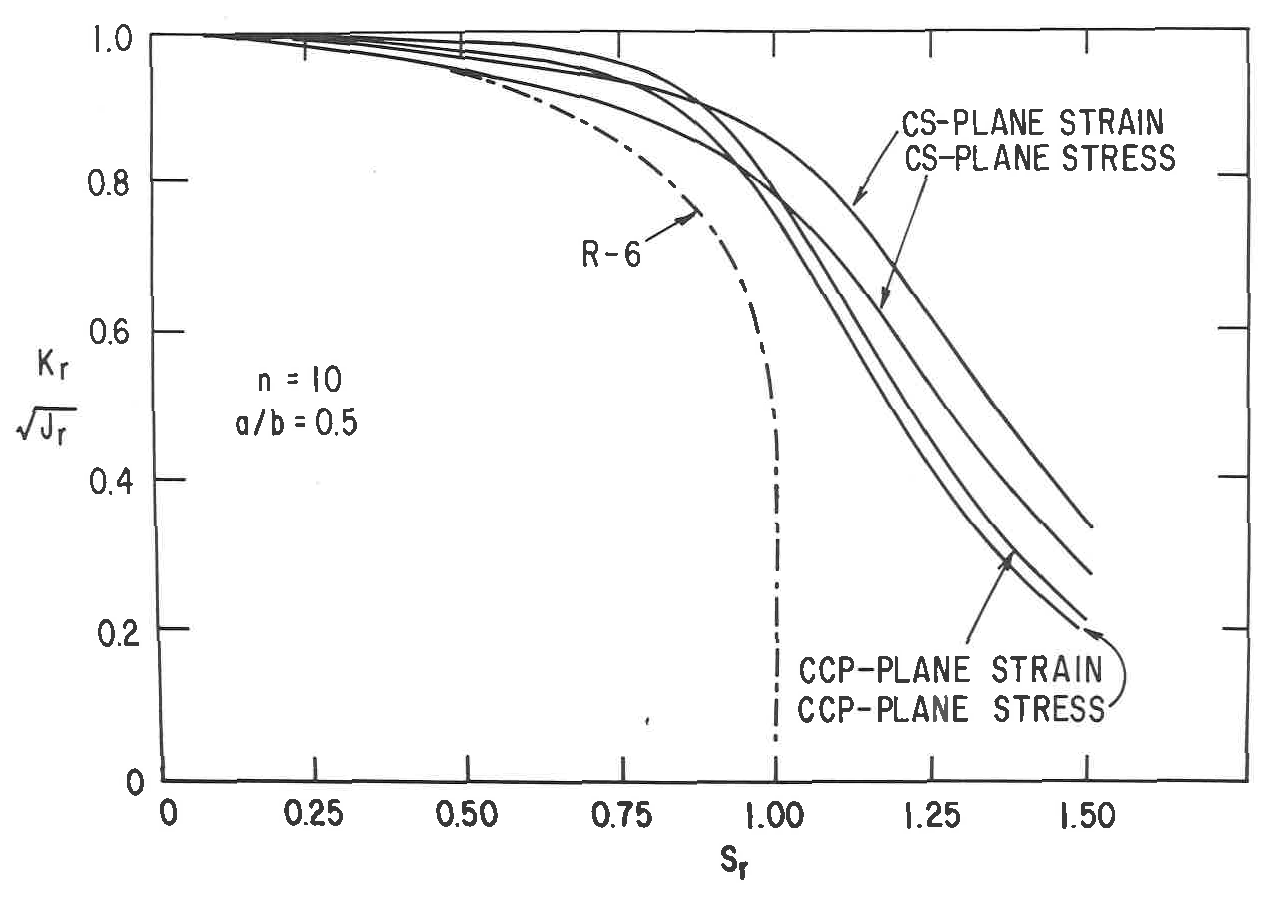
\includegraphics[width=0.7\columnwidth]{FAD-variance-geometry-modified}
\caption[Failure assessment diagram of center-cracked panel and compact tension specimen]{\label{fig:fad-ccp-ct} Failure assessment diagram of center-cracked panel and compact tension specimen \cite{epri1981}}
\end{figure}
The effect of crack length on a plane strain center-cracked panel with \(n = 10\) is shown in \Cref{fig:fad-crack-lengths}.
\begin{figure}
\centering
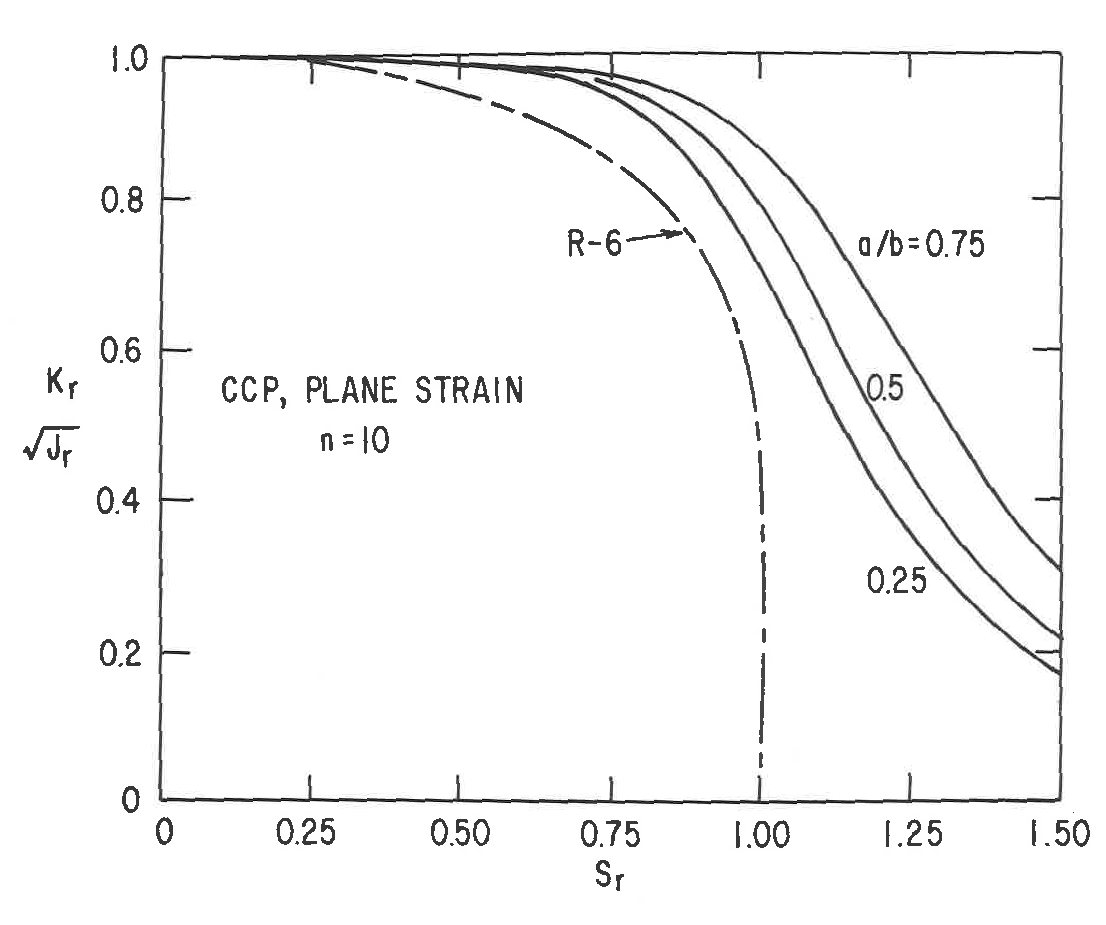
\includegraphics[width=0.7\columnwidth]{FAD-variance-aW-modified}
\caption[Failure assessment diagram of center-cracked panel with multiple crack sizes]{\label{fig:fad-crack-lengths} Failure assessment diagram of center-cracked panel with multiple crack sizes \cite{epri1981}}
\end{figure}

\subsection{Failure Assessment Diagrams using Reference Stress Model}

In general, materials can not always be accurately characterized with a power-law curve fit.
But given stress-strain data and the flow stress \(\sigma_0\), \citet{ainsworth1984} defined a reference stress \(\sigma_\textnormal{ref}\) as
\begin{align}
\sigma_\textnormal{ref} &= \frac{P}{P_0}\sigma_0
\end{align}
and a corresponding reference strain \(\epsilon_\textnormal{ref}\) is the total axial strain resulting from applying a uniaxial stress of \(\sigma_\textnormal{ref}\).
Using these values to calculate \Jpl results in
\begin{align}
\Jpl &= \sigma_\textnormal{ref} b \hone \left( \epsilon_\textnormal{ref} - \frac{\sigma_\textnormal{ref} \epsilon_0}{\sigma_0} \right),
\end{align}
where \hone is a dimensionless function of geometry and the power-law exponent \(n\) defined in the EPRI technical report NP-1931 ``Engineering Approach for Elastic-Plastic Fracture Analysis'' \citep{epri1981}.
Though \hone is a function of \(n\), Ainsworth approximated \(\hone(n) \approx \hone(1)\), the \hone value for a linear material.
Though less accurate for low-hardening materials (large values for \(n\)), these materials are already accurately modeled with the simpler strip-yield model.
Ainsworth's approximation for high-hardening materials leads to a simpler \Jpl in terms of the linear elastic stress intensity factor \KI:
\begin{align}
\Jpl &= \frac{\mu \KI^2}{E} \left( \frac{E \epsilon_\textnormal{ref}}{\sigma_\textnormal{ref}} - 1 \right)
\label{eq:jpl-ainsworth}
\end{align}
where \(\mu = 0.75\) for plane strain conditions, and \(\mu = 1.0\) for plane stress conditions.
As \KI values are much more readily found in literature than \hone values, Ainsworth's \Jpl formula can be simpler than EPRI models.

\subsection{Harmonization of Fitness for Purpose Standards}

Each FFP standard attempted to account for multiple modes of structural failure, and experience gained from use of each standard led to the development of encompassing standards with multiple levels of assessment, depending on factors including acceptable levels of conservatism, material type, and available material property data.

While the R6 approach was being developed using strip yield behavior, the British Standards Institute\nomenclature[1B]{BSI}{British Standards Institute} was developing an analogous guide (PD~6493) \cite{pd6493-1991} relating stress to a CTOD-based measurement of fracture toughness and discontinuity size.
Though the initial PD~6493 design curves were conservative in the vast majority of cases, resulting factors of safety ranged from below 1 to over 10 \citep{anderson2005}.
The PD~6493 standard also required separate analysis to determine if the structure was more susceptible to plastic collapse instead of brittle fracture.

A second revision of PD~6493 in 1991 incorporated three levels of assessment, from simplest to most complex.
The Level 1 preliminary assessment added a FAD to the CTOD criteria, so that plastic collapse checks were integrated into the document.
The Level 2 normal assessment was similar to the second edition R6 method, and the Level 3 advanced assessment adapted methods from the third edition R6 standard, including considerations of ductile crack extension \citep{WIESNER2000883}.

In 1999, PD~6493 was converted into a British Standard and designated BS~7910 \cite{bs7910-1999}, and has undergone further revisions and harmonization with other standards including the European FITNET program.
As of 2015 (the latest revision of BS~7910), the ``Level'' terminology was replaced with ``Option'' terminology, and the simplest Level~1 procedure was removed entirely.
Option~1 is conservative, and only requires material data for elastic modulus, yield strength, and ultimate strength.
Option~2 requires a true stress-strain curve, and Option~3 requires use of the \J integral.
Also in the 2015 revision, if crack-tip constraint (the restriction of Poisson effects due to geometry or hydrostatic stress state) can be assessed, it can influence the values used for fracture toughness, and can also affect the equations used to construct the FAD.
These constraint modifications can be applied at any of the three options.
Further background material on constraint and its influence on fracture criteria follows in the next section.

\section{Constraint and Two-Parameter Fracture}

Throughout the preceding section, stress intensity factors, fracture toughness measures, and other quantities have shown a dependency on specimen geometry and plane stress or plane strain conditions, including
plastic zone sizes in \Cref{eq:ry,eq:rp}, \(\frac{a}{W}\) FADs in \Cref{fig:fad-crack-lengths}, and \(\mu\) values in \Cref{eq:jpl-ainsworth}.
These variations are more prominent in the presence of significant plastic deformation, and can be traced back to a general concept of constraint.

Constraint results from conditions that limit or constrain out-of-plane deformation and strain.
Perfectly plane strain conditions are completely constrained in the out-of-plane direction, while perfectly plane stress conditions are completely unconstrained in the out-of-plane direction.
Along the perimeter of a surface crack, the free surface shows little to no constraint, and locations deep within the crack front show higher constraint.

Constraint can also be correlated to the level of stress triaxiality, since large out-of-plane stresses are required to counteract the Poisson's effect that would cause out-of-plane deformation and strain.
Since metals in a plastic state behave similarly to incompressible fluids (\(\nu = 0.5\) instead of \(\nu \approx 0.3\) for an elastic state), this has the effect of limiting the plastic zone size in regions of high constraint.
Higher constraint leads to lower fracture toughness measurements, as a reduced plastic zone size limits ductile behavior of the metal, effectively making it more brittle.

\citet{williams1957} developed an infinite power series form of stress fields near a crack tip of the form
\begin{align}
\sigma_{ij} &= O(r^{-\frac{1}{2}}) + O(r^0) + O(r^{\frac{1}{2}}) + O(r^{\frac{1}{2}}) + \cdots
\end{align}
where the first term is of the form of \Cref{eq:singularity} and dominates the stress values closest to the crack tip.
The third and higher terms in the Williams series vanish near the crack tip, but the second term remains constant, and affects the stress field for values of \(r\) where the magnitude of the singularity term is reduced.

The first two terms of the Williams series for the stress state of a plane strain body subject to Mode I loading are
\begin{align}
\sigma_{ij} &= \frac{\KI}{\sqrt{2\pi r}} f_{ij}(\theta) +
\begin{bmatrix}
T & 0 & 0 \\
0 & 0 & 0 \\
0 & 0 & \nu \T
\end{bmatrix}
\label{eq:t-stress}
\end{align}
where \T is a stress in the \(x\) direction that is a function of the geometry and applied loading, that in turn induces a stress \(\nu \T\) in the \(z\) direction due to plane strain assumptions \citep{anderson2005}.
The single-parameter stress field of \Cref{eq:singularity} where \(\T = 0\) only applies in the limiting case where the plastic zone size is tiny compared to the crack size and the size of the body.

For other cases (\(\T \neq 0\)), \citet{cr5970} performed a modified boundary layer analysis of the region surrounding the crack tip.
Variations in \T affected the \(y\) direction stresses, with \(\T=-\sigma_0 \) values reducing stresses by up to 45\% as shown in \Cref{fig:mbl}.
\begin{figure}
\centering
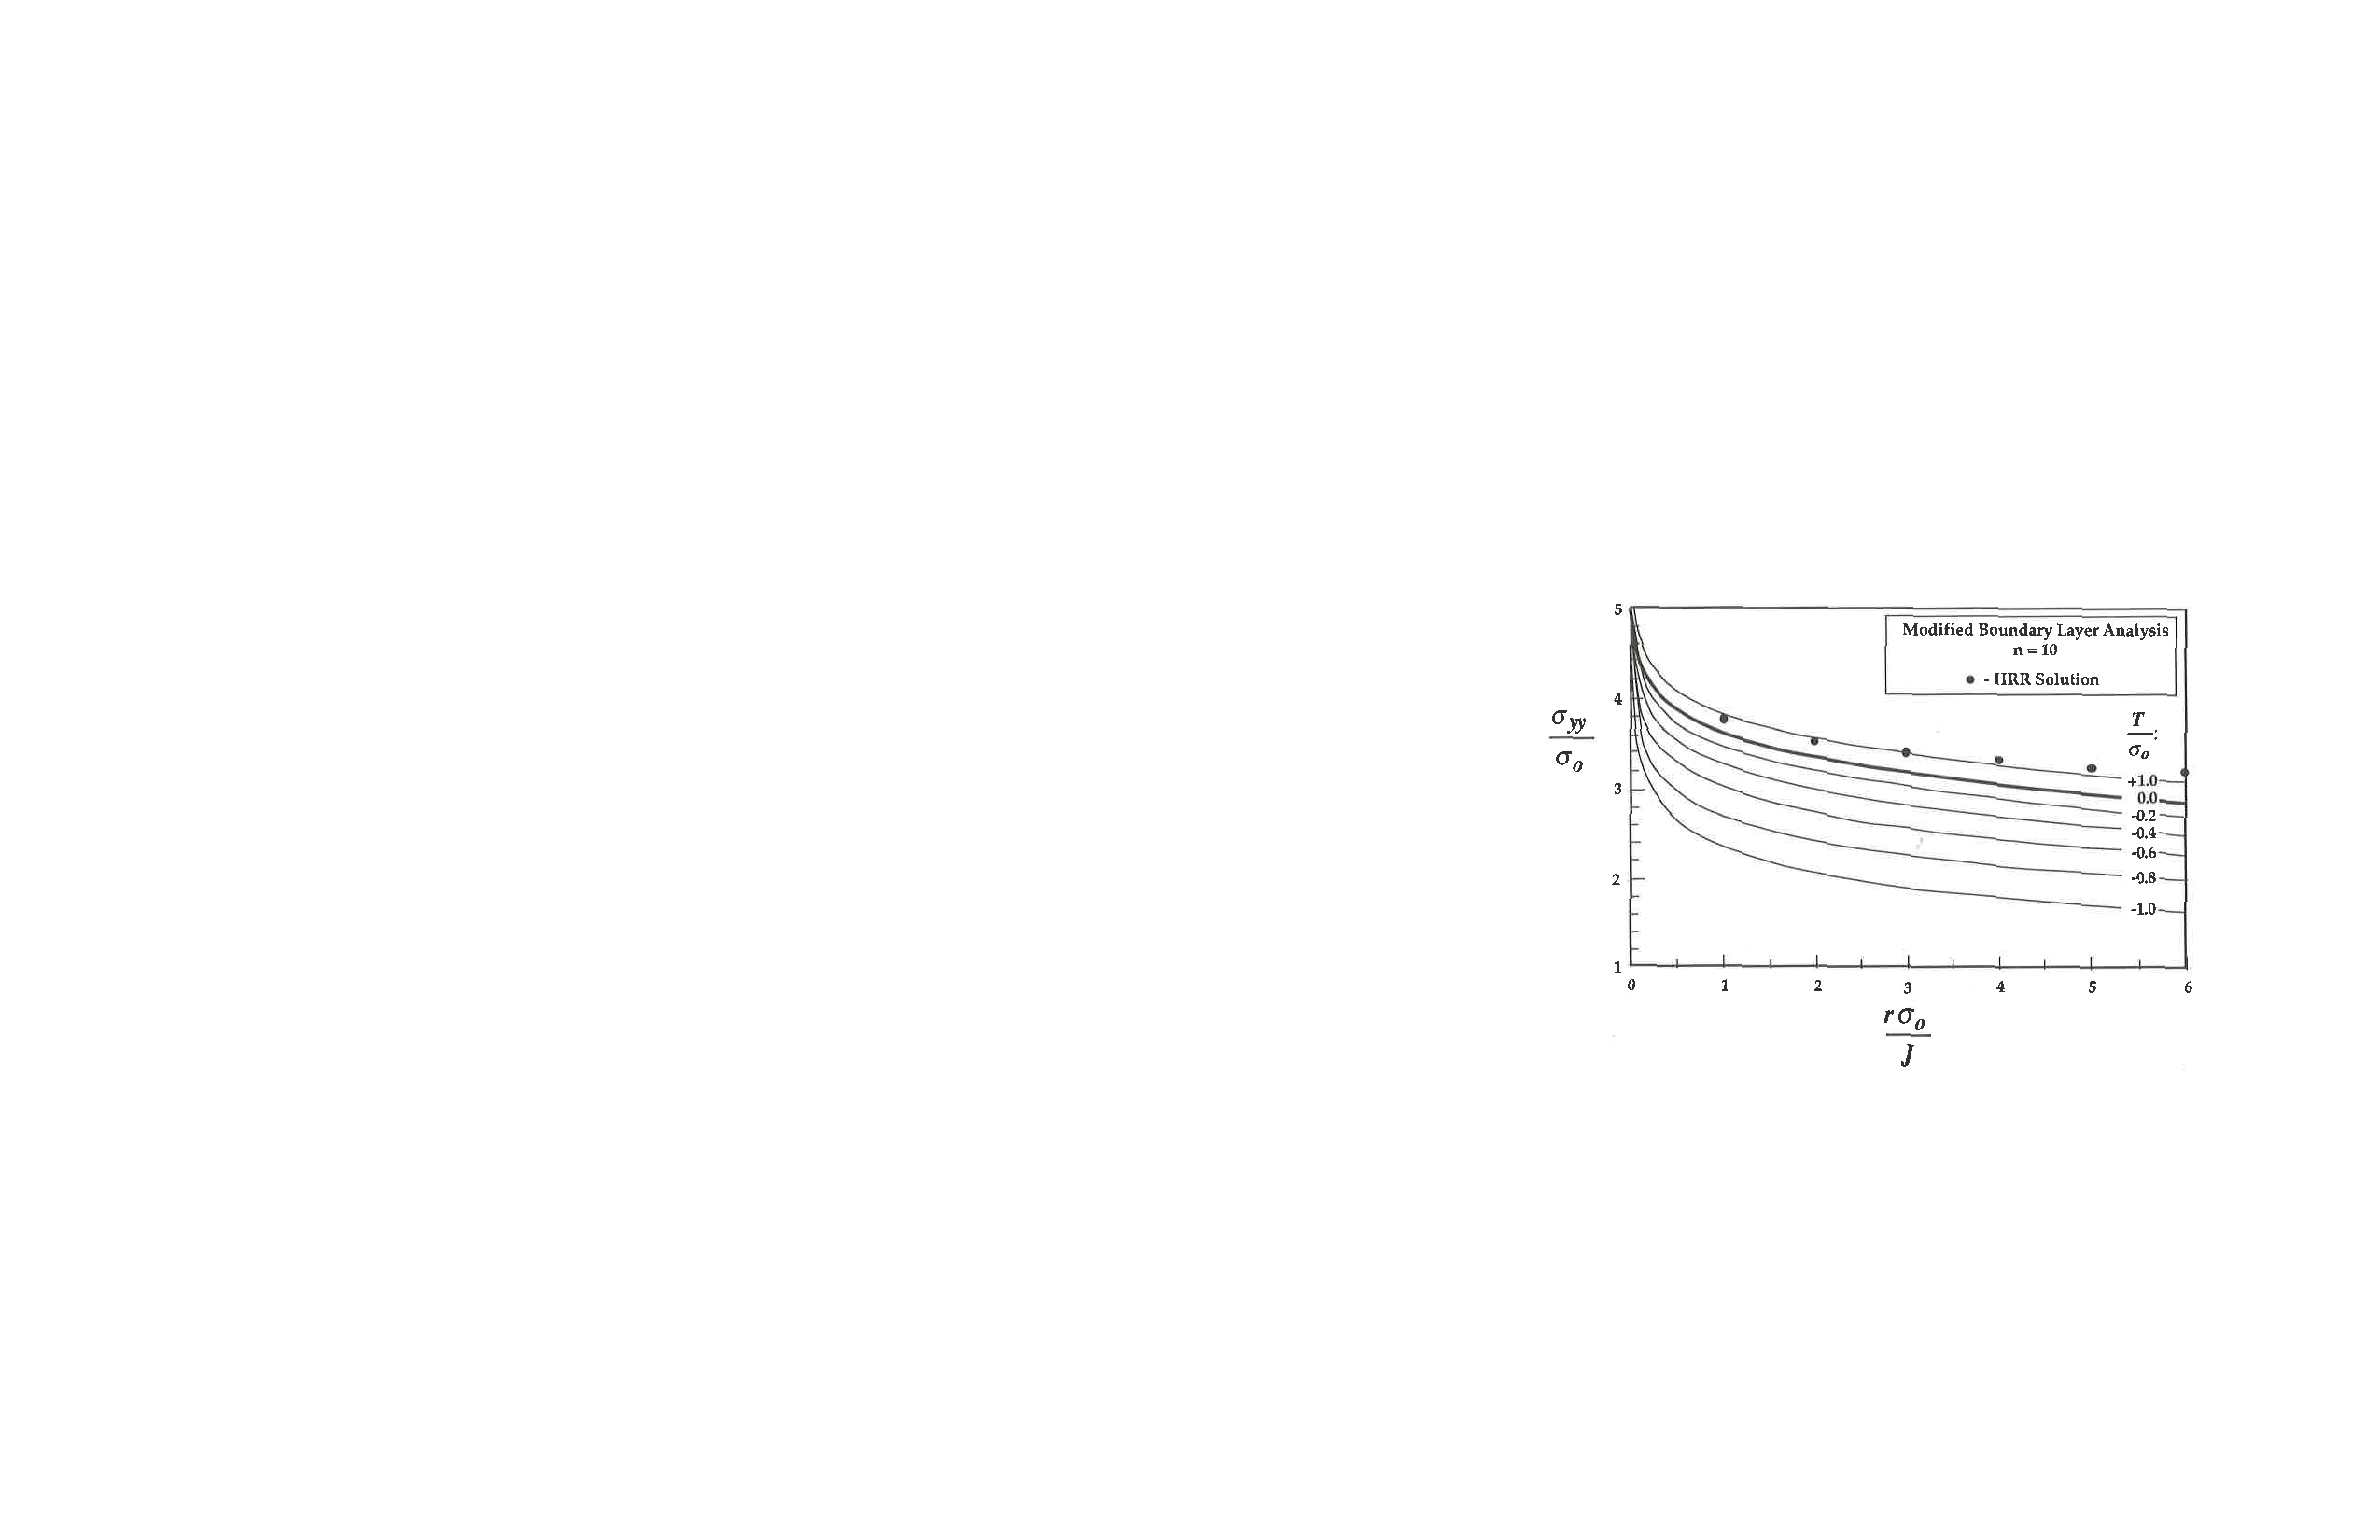
\includegraphics[width=0.8\columnwidth]{stress-mbl}
\caption[Stress fields from modified boundary layer analysis]{\label{fig:mbl} Stress fields from modified boundary layer analysis \citep{anderson2005}}
\end{figure}
As \T scales with applied stress similarly to \KI, a non-dimensional measure of stress biaxiality \(\Be\) can be defined as
\begin{align}
\Be &= \frac{T \sqrt{\pi a}}{\KI}
\end{align}
and is only a function of cracked body configuration and relative crack size as shown in \Cref{fig:biaxiality}.
\begin{figure}
\centering
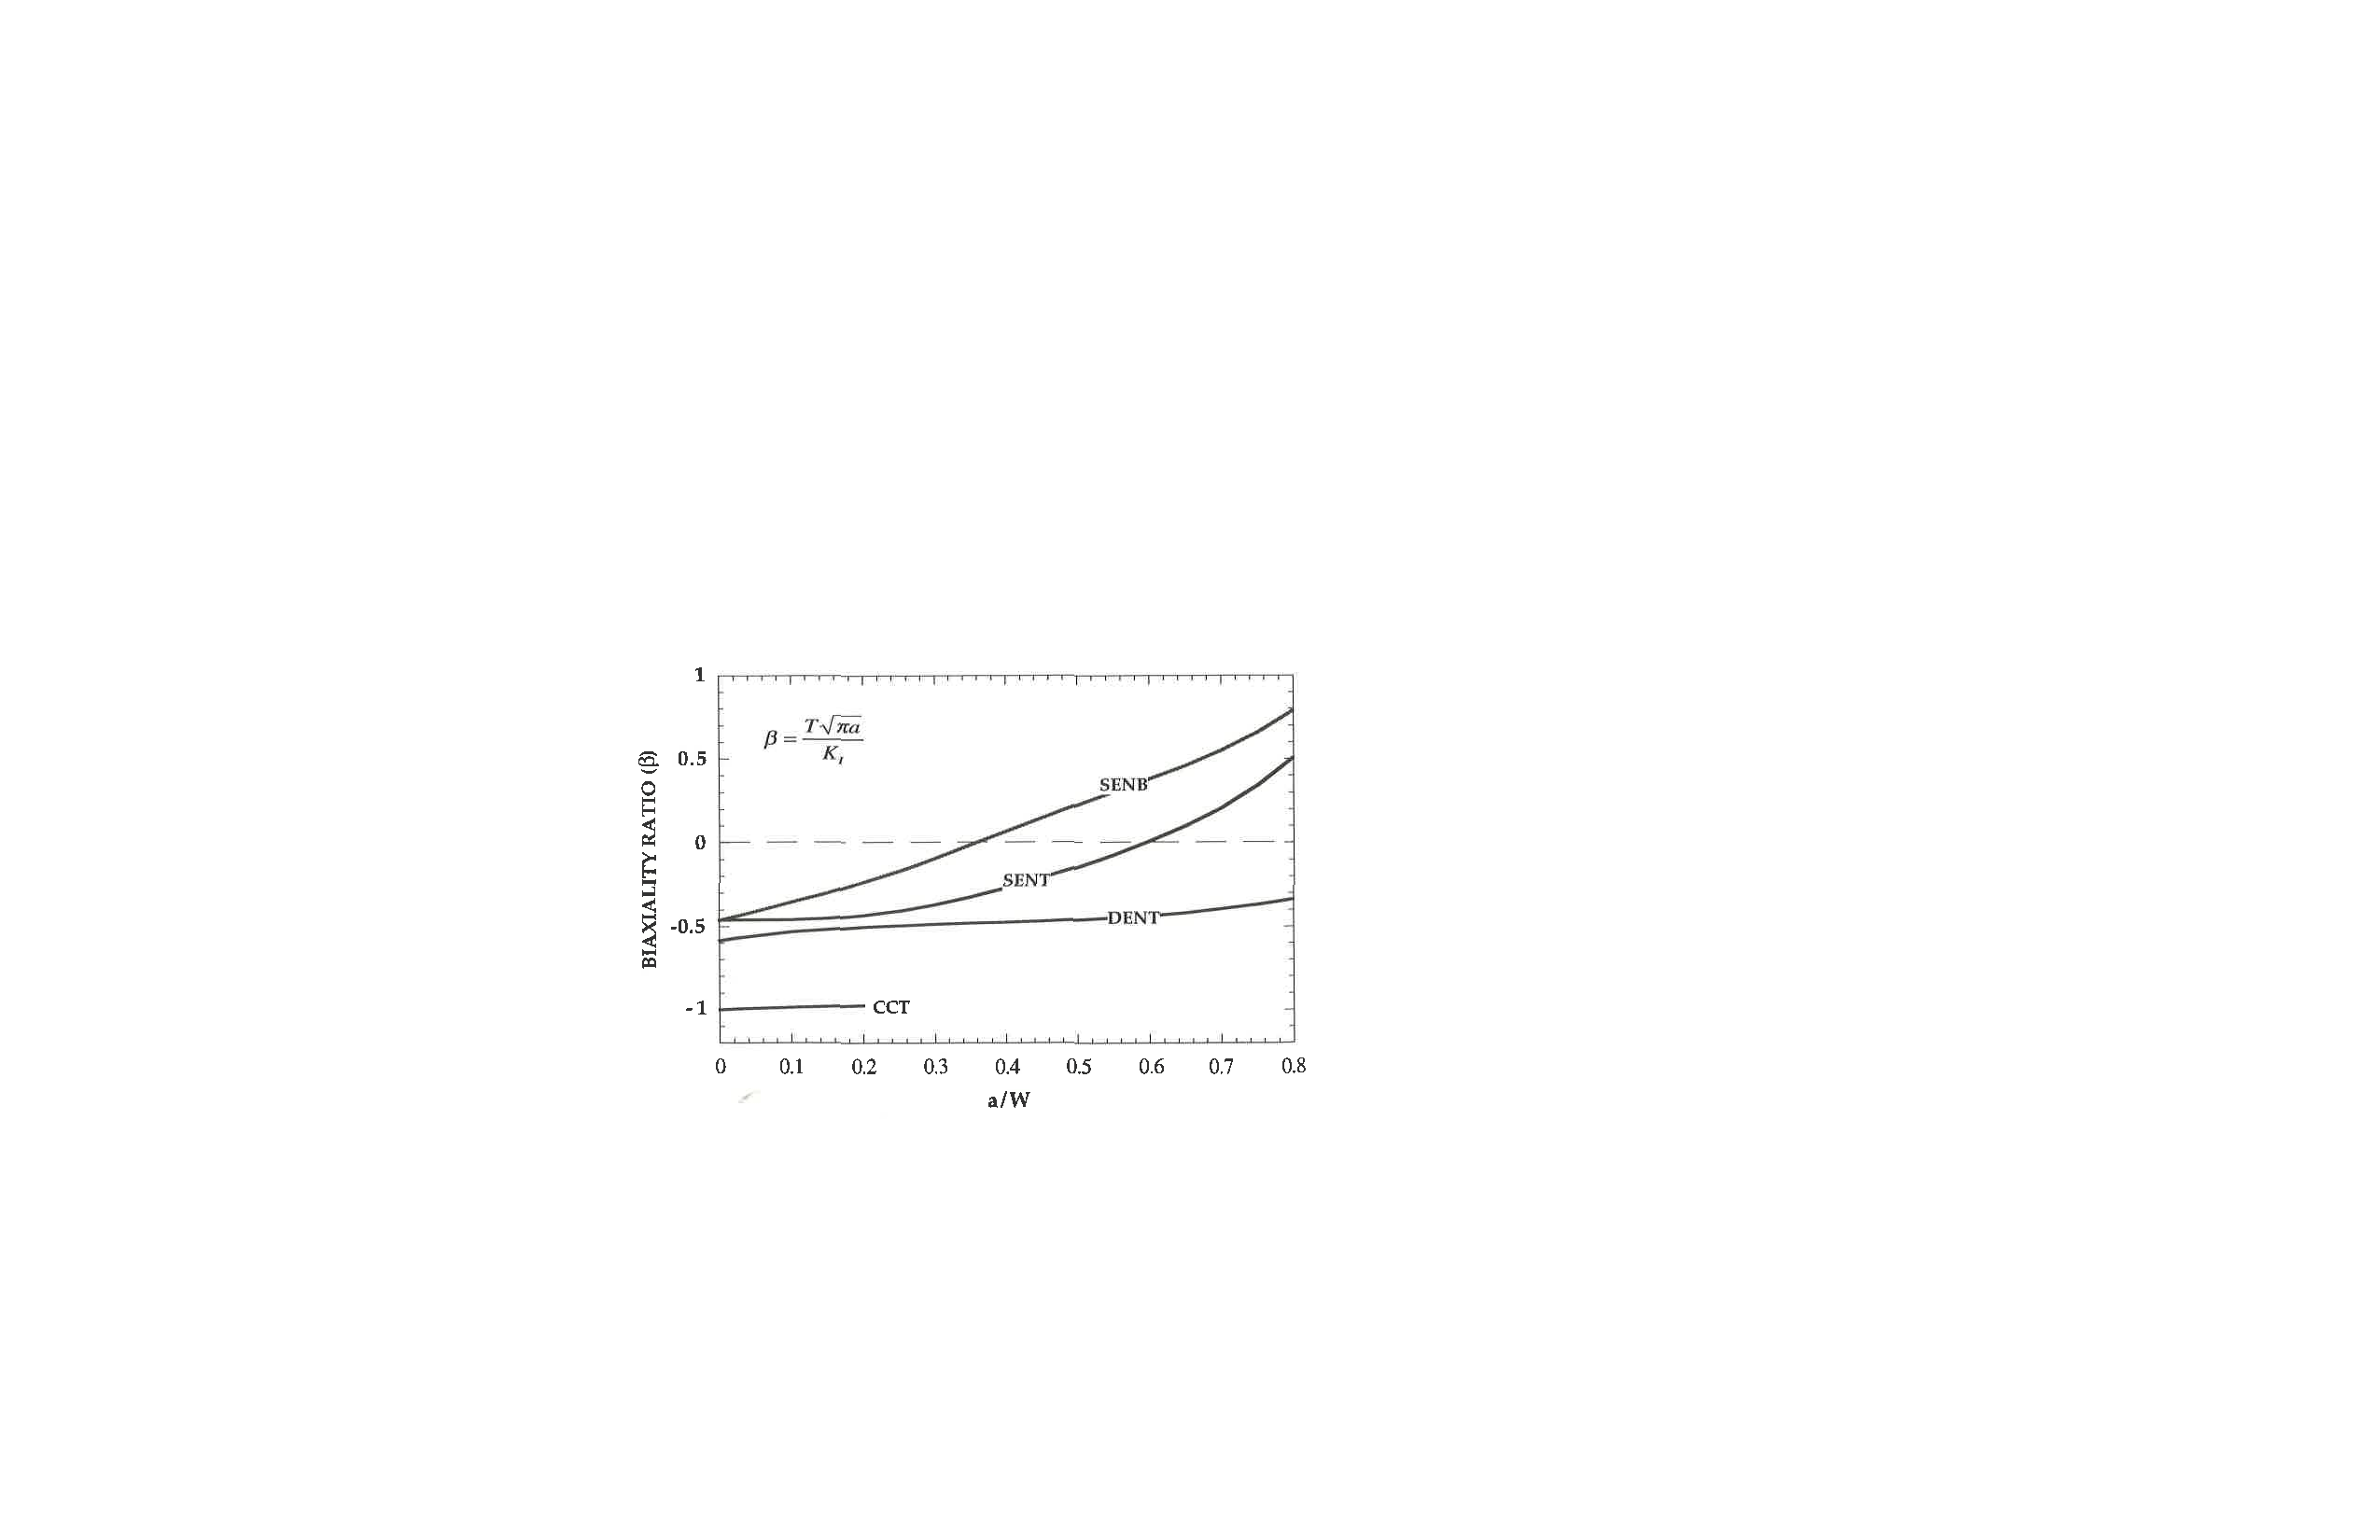
\includegraphics[width=0.8\columnwidth]{biaxiality}
\caption[Biaxiality ratio for various cracked body geometries and loading conditions]{\label{fig:biaxiality} Biaxiality ratio for various cracked body geometries and loading conditions \citep{anderson2005}}
\end{figure}

The stress state from \Cref{fig:mbl} could be written as either
\begin{align}
\Sigij &= \left( \Sigij \right)_\textnormal{HRR} + \left( \Sigij \right)_\textnormal{Diff}
\intertext{or}
\Sigij &= \left( \Sigij \right)_{T=0} + \left( \Sigij \right)_\textnormal{Diff} \label{eq:difference-field}
\end{align}
where \(\left( \Sigij \right)_\textnormal{Diff}\) is the difference between \Sigij and the corresponding baseline stress state.
For the second case, using \(\left( \Sigij \right)_{T=0}\) as the baseline, it can be seen that
\(\left( \Sigij \right)_\textnormal{Diff}\)
is relatively constant with respect to distance from the crack tip.
\citeauthor{odowdshih1991} \cite{odowdshih1991, odowdshih1992} extended that approximation to all points forward of the crack tip.
Additionally, they found that
\begin{gather}
\left( \Sxx \right)_\textnormal{Diff} \approx \left( \Syy \right)_\textnormal{Diff}
\gg \left( \sigma_{xy} \right)_\textnormal{Diff}
\end{gather}
indicating that the \T stress effectively causes a hydrostatic shift in stress ahead of the crack tip, dependent on a single parameter \Q.
Thus, \Cref{eq:difference-field} can be rewritten as
\begin{align}
\Sigij &= \left( \Sigij \right)_{T=0} + Q \Szero \deltaij \label{eq:Q-field}
\end{align}
where \deltaij is the Kronecker delta.
\Q has typically been calculated as
\begin{align}
\Q &= \frac{\Syy - \left(\Syy\right)_{T=0}}{\Szero} \text{\quad at } \theta = 0 \text{ and } \frac{r \Szero}{\J} = 2.
\end{align}
\Q and \T have a one-to-one relationship at a given hardening exponent \(n\) as shown in \Cref{fig:q-vs-t}, and \Cref{fig:q-vs-J} shows that \Q remains close to the small-scale yielding value of 0 over a wide range of deformations for bend specimens, versus rapidly dropping with any deformation for center-cracked specimens.

The trend of critical \J values over a range of constraint conditions is shown in \Cref{fig:j-q-experiments}.
Though considerable scatter is present, there is a clear trend that negative \Q values (and correlated negative \T stresses) lead to higher fracture toughness measurements when the failure mechanism is stress-controlled.
As the crack driving force increases, fracture will occur as the \J-\Q curve passes through the shaded region of \Cref{fig:j-q-application}.
\begin{figure}
\centering
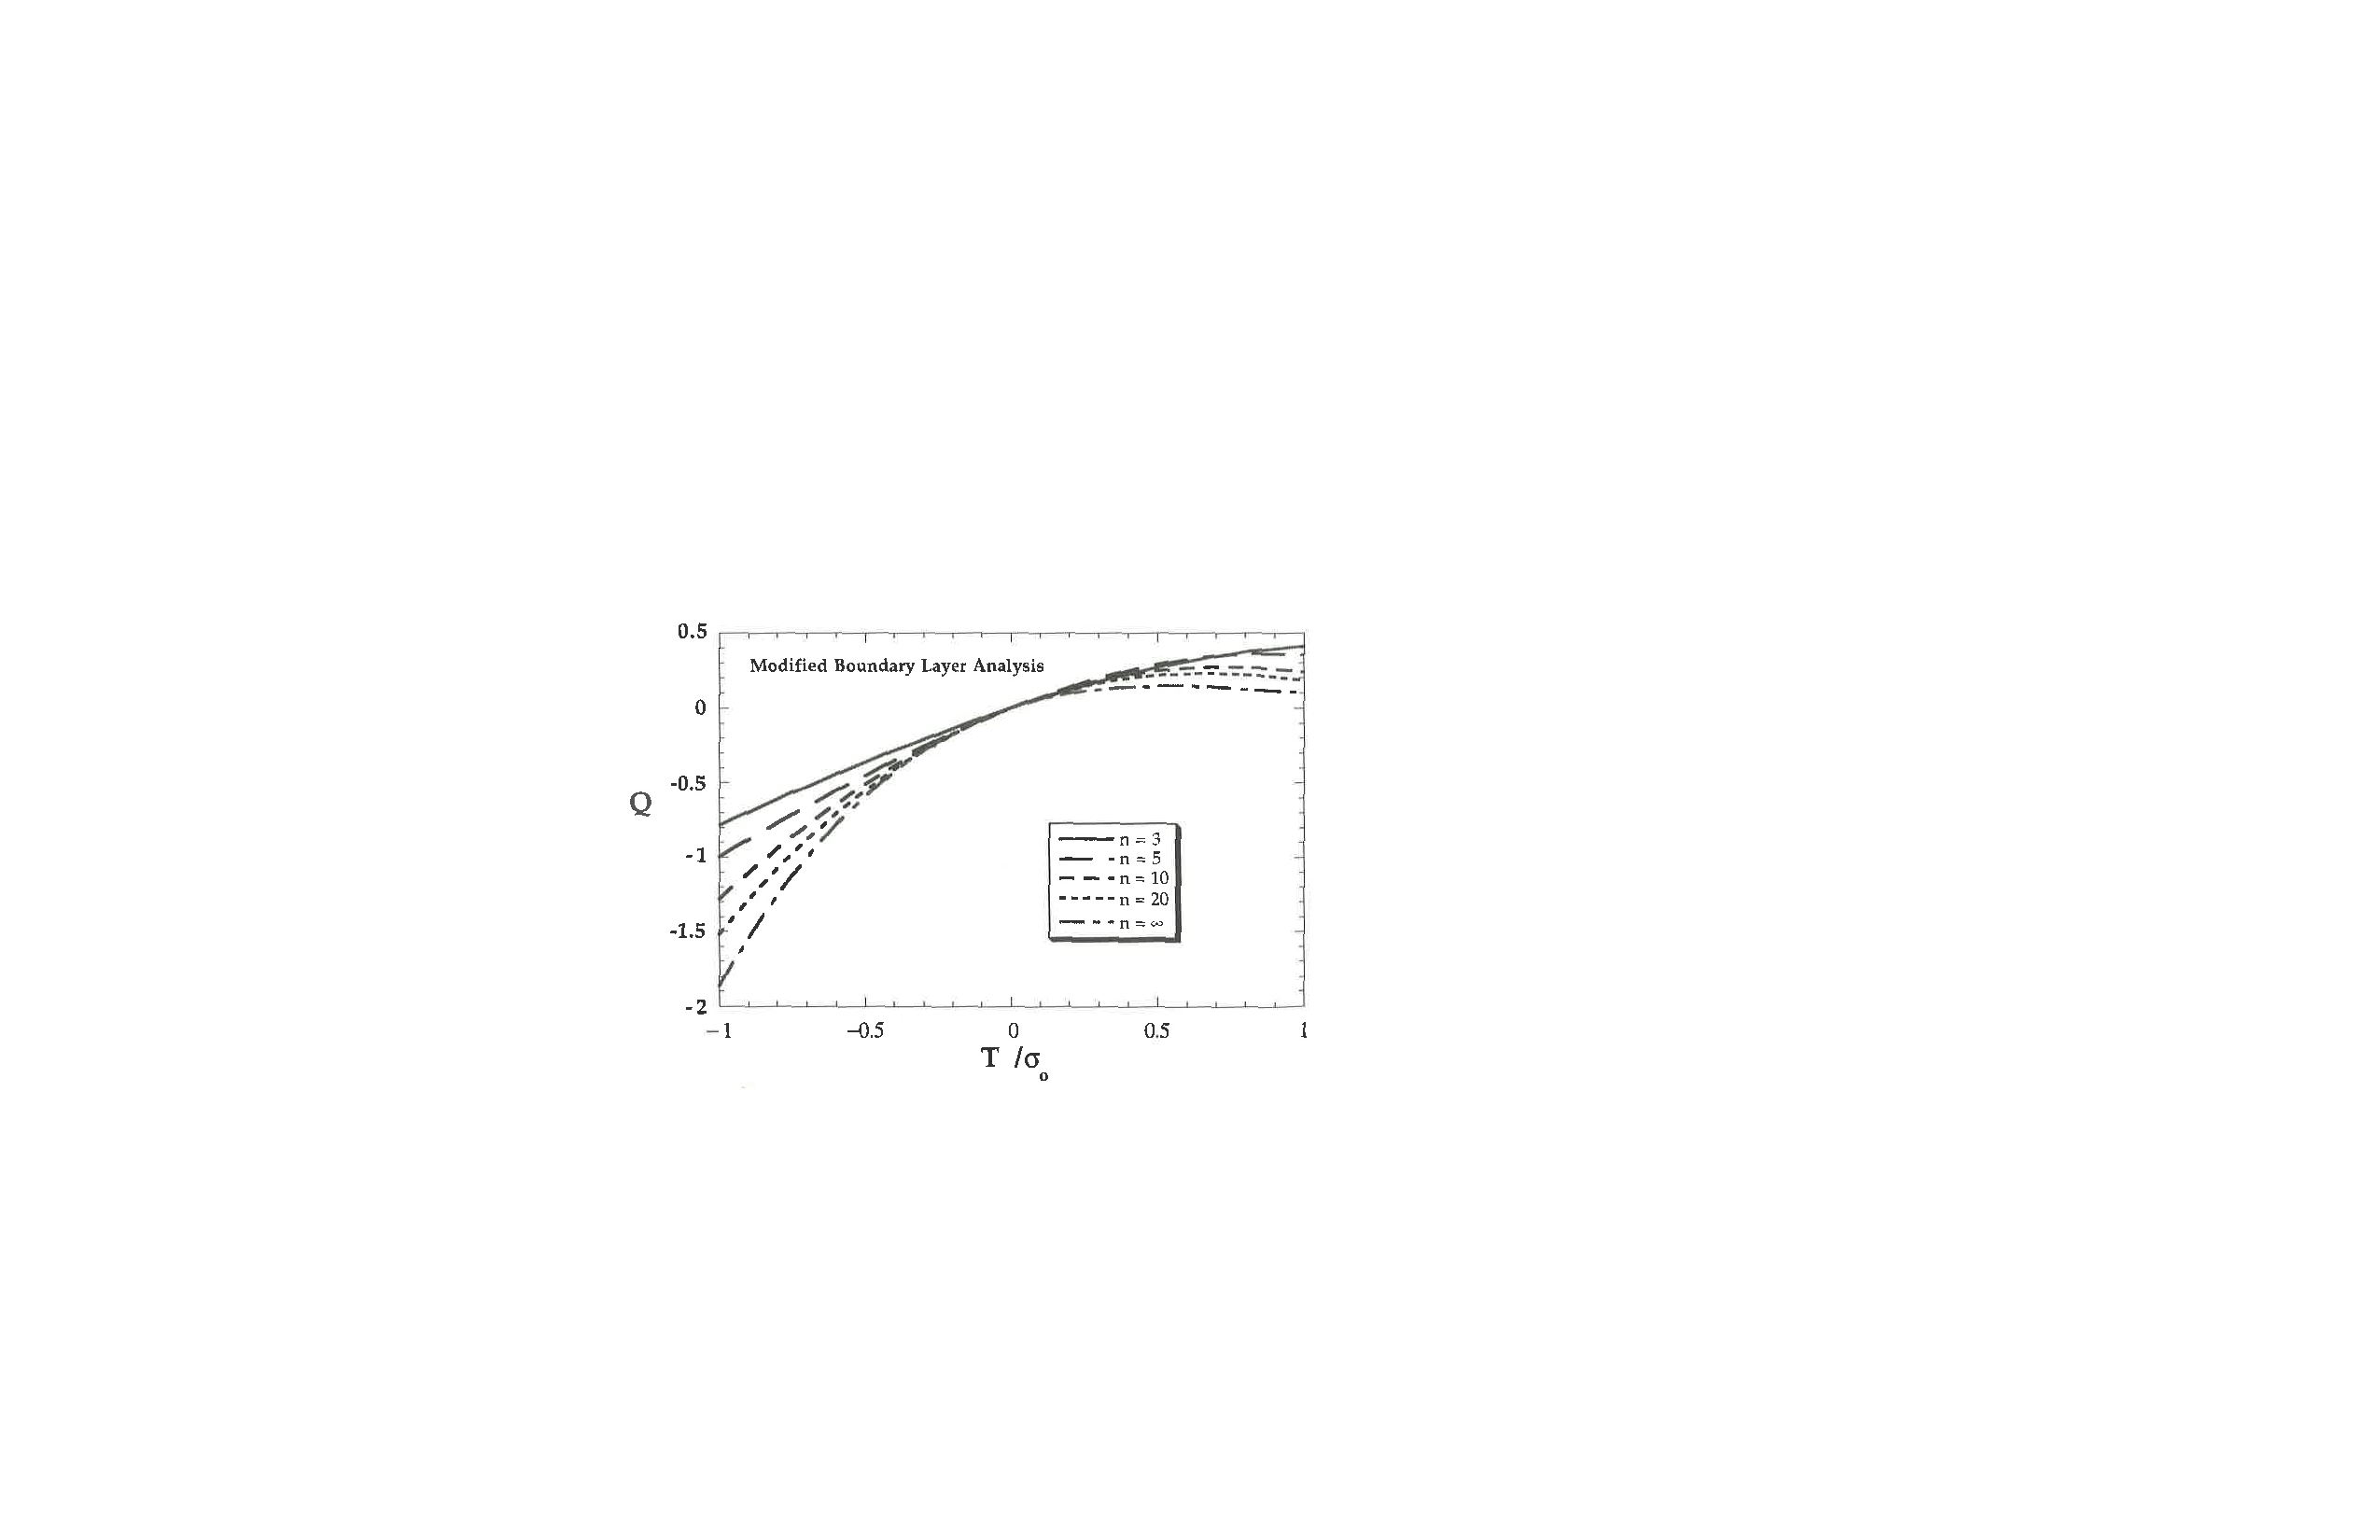
\includegraphics[width=0.7\columnwidth]{q-t}
\caption[Relationship between \Q and \T as a function of hardening exponent \(n\)]{\label{fig:q-vs-t} Relationship between \Q and \T as a function of hardening exponent \(n\) \citep{anderson2005}}
\end{figure}
\begin{figure}
\centering
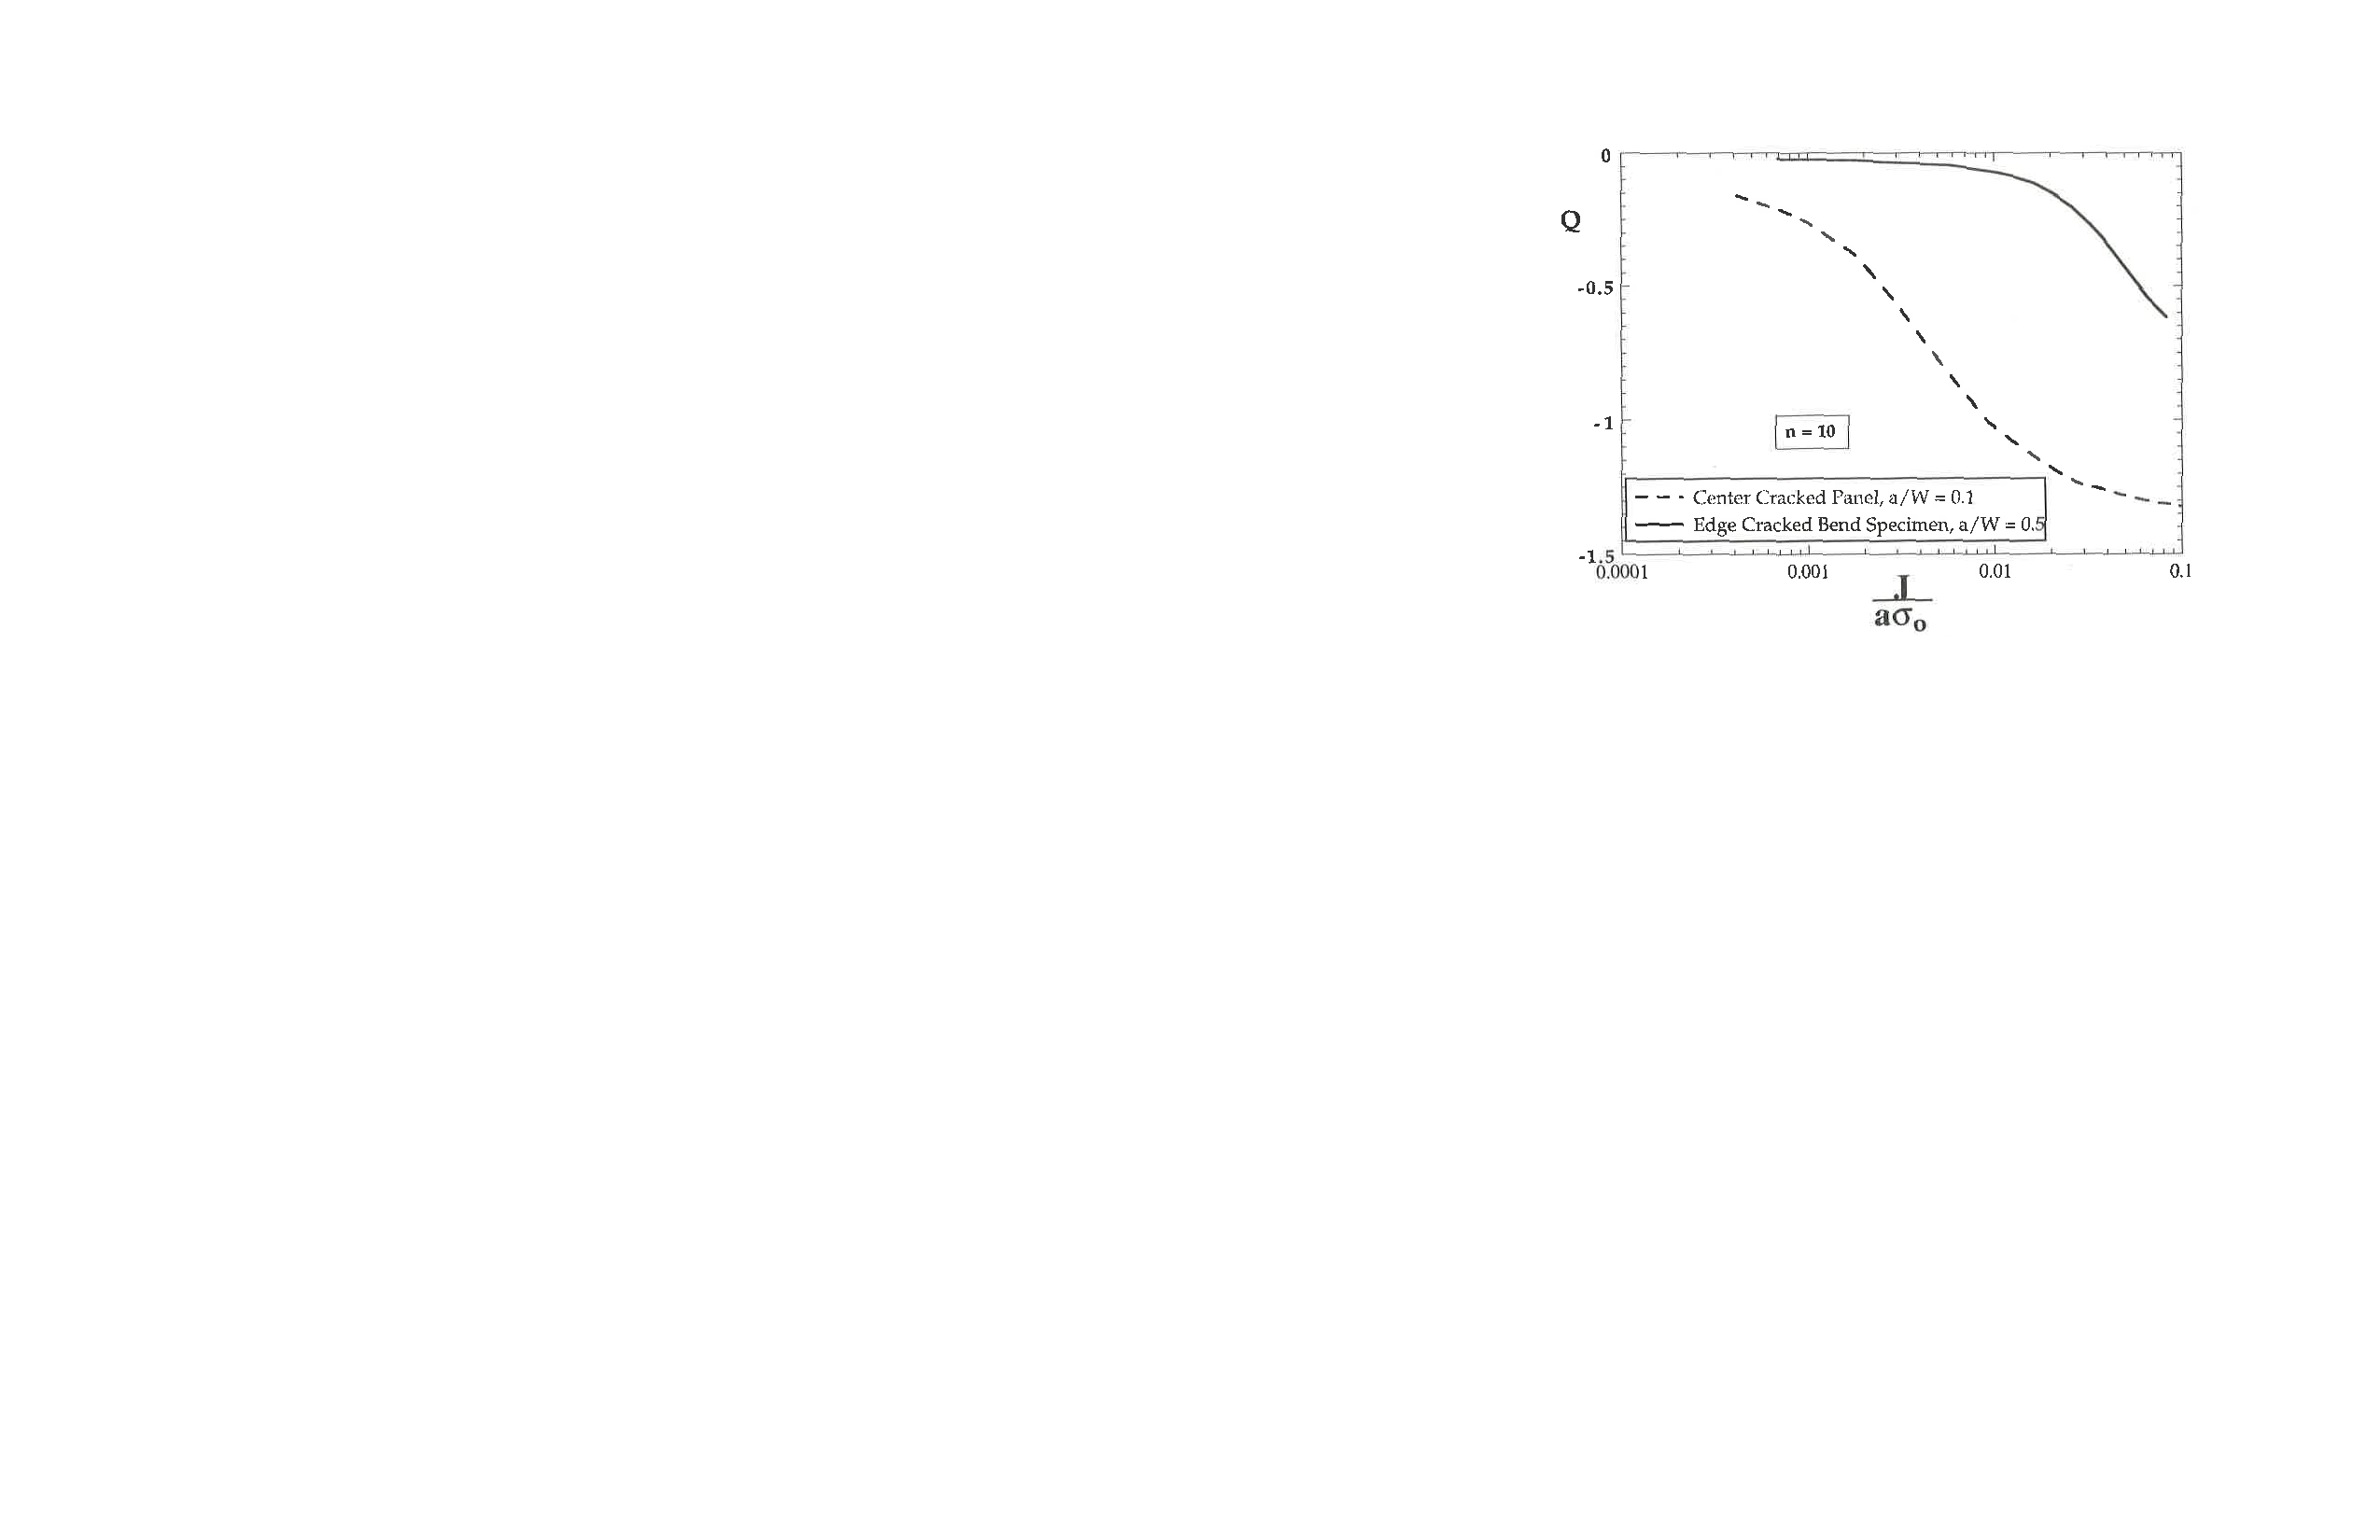
\includegraphics[width=0.7\columnwidth]{q-deflection}
\caption[Relationship between \Q and \J as for two geometries]{\label{fig:q-vs-J} Relationship between \Q and \J as for two geometries \citep{anderson2005}}
\end{figure}
\begin{figure}
\centering
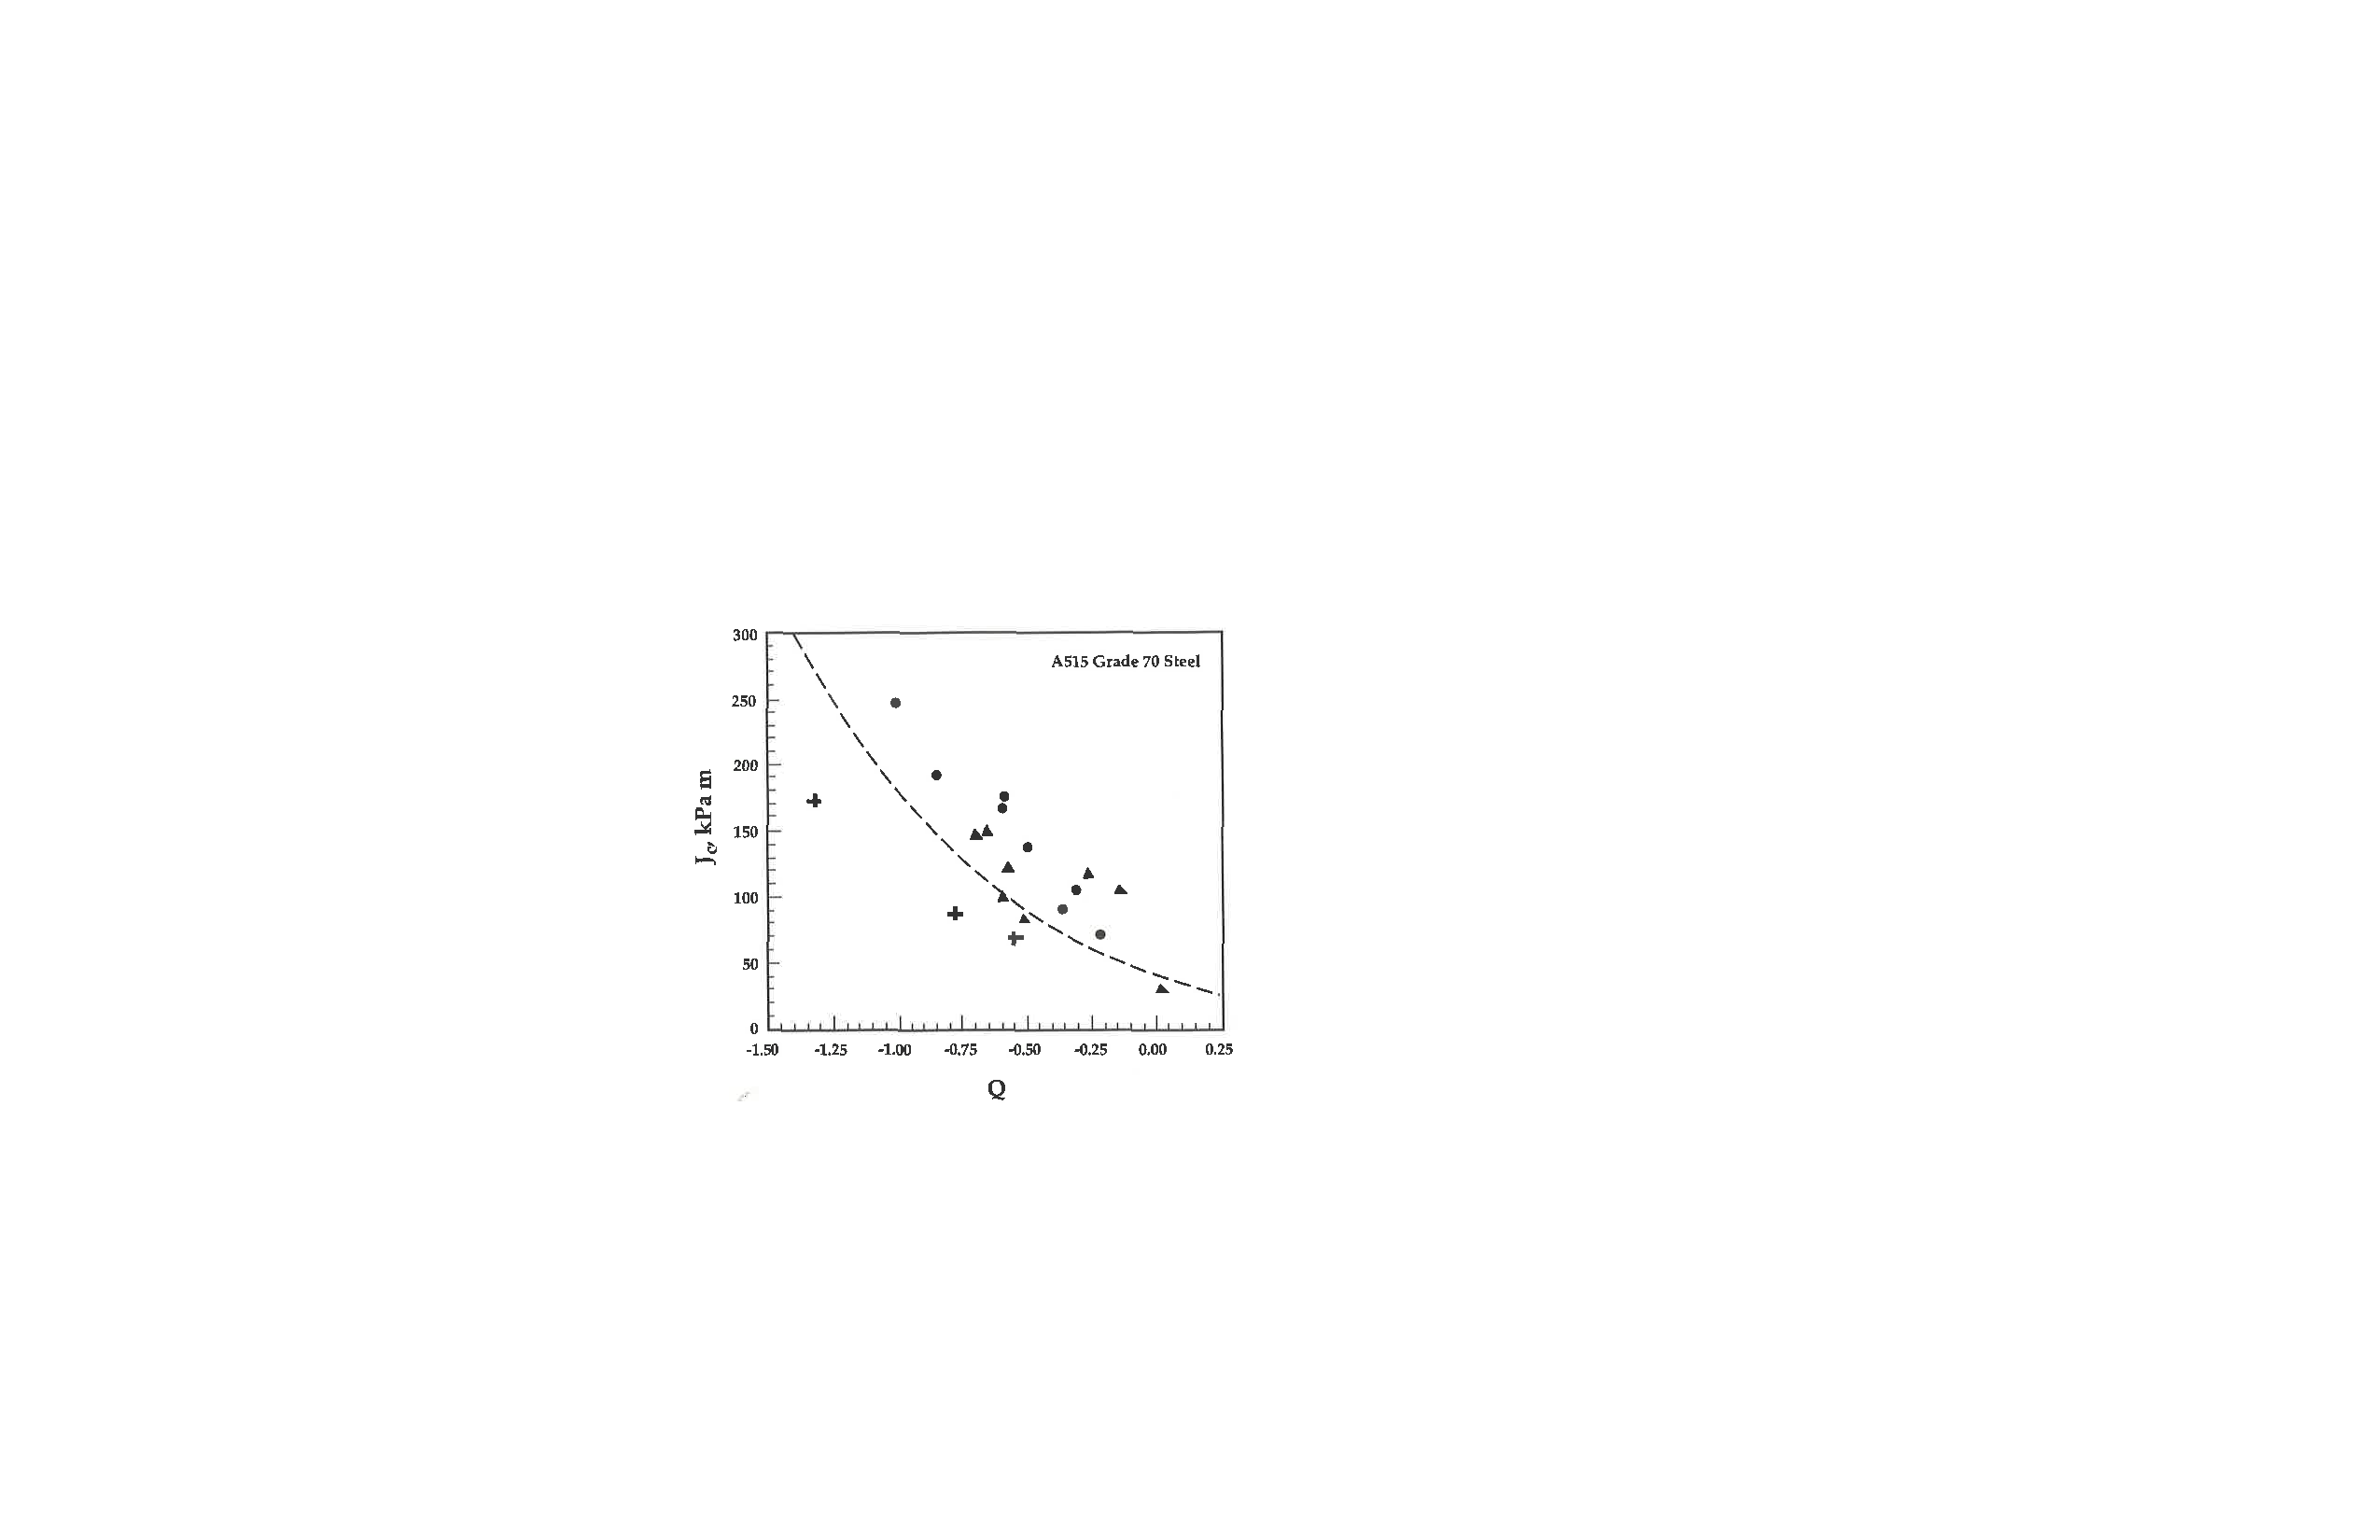
\includegraphics[width=0.7\columnwidth]{j-q-experiments}
\caption[Experimental \J values over a range of \Q values]{\label{fig:j-q-experiments} Experimental \J values over a range of \Q values \citep{anderson2005}}
\end{figure}
\begin{figure}
\centering
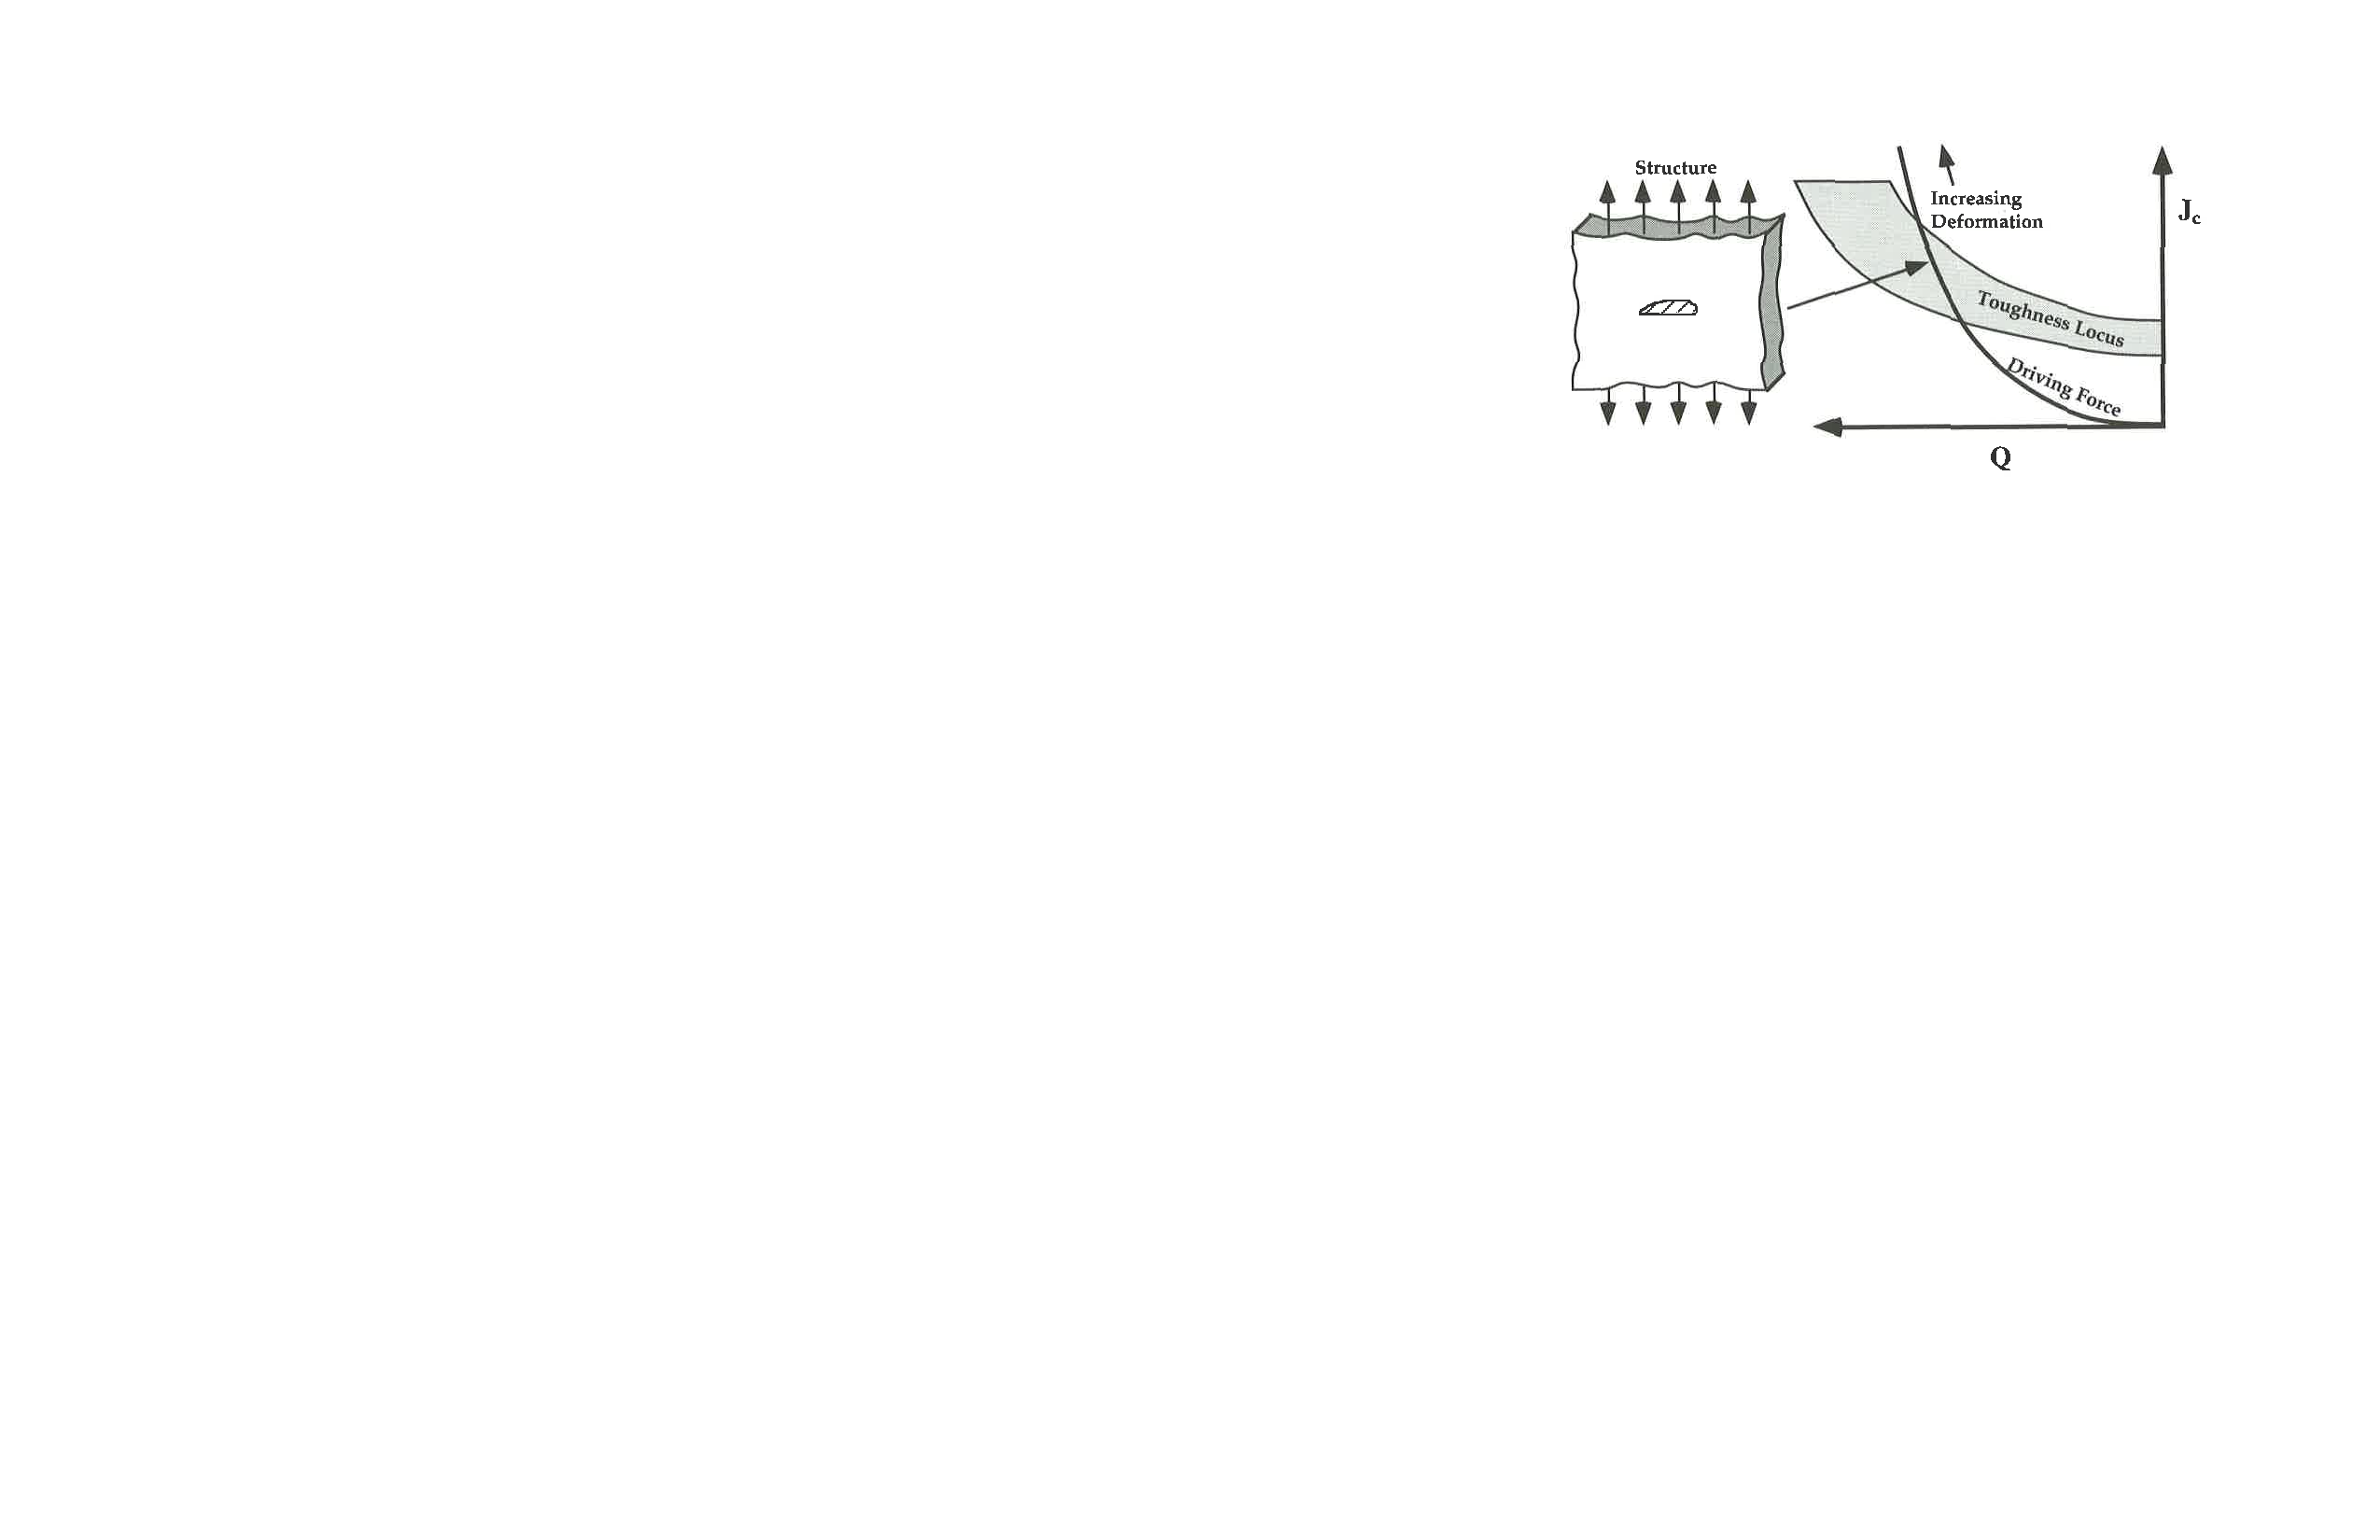
\includegraphics[width=0.7\columnwidth]{j-q-application}
\caption[\J-\Q locus]{\label{fig:j-q-application} \J-\Q locus \citep{anderson2005}}
\end{figure}

\FloatBarrier
\section{Methods for Elastic-Plastic and Fully-Plastic Bending Analysis}

This section will detail a selection of methods used to calculate or estimate \J, both numerically and experimentally.
These methods include the adaptation of the contour integral form of \J to a domain integral formulation suitable for finite element analysis, handbook and tabular methods for calculating \J and \K, and the load separation technique for estimating \J from experimental load-displacement records.

\subsection{Numerical Methods}

Though \J is commonly expressed as a contour integral as in \Cref{eq:j-contour-integral}, that formulation does not easily lend itself to numerical evaluation for finite element analysis.
The contour integral form of \J can be rewritten as an equivalent domain integral for a discretized finite element model, as shown in \cite{anderson2005,warp3d,doddsvargas1988}.
For a surface crack model in three dimensions, the domain is a volume of elements surrounding a particular point on the crack front, with a local coordinate system (\(x_1, x_2, x_3\)) with its origin at the crack tip and the \(x_1\) direction oriented toward the direction of crack extension as shown in \Cref{fig:domain-integral-volume}.
\begin{figure}[tbp]
\centering
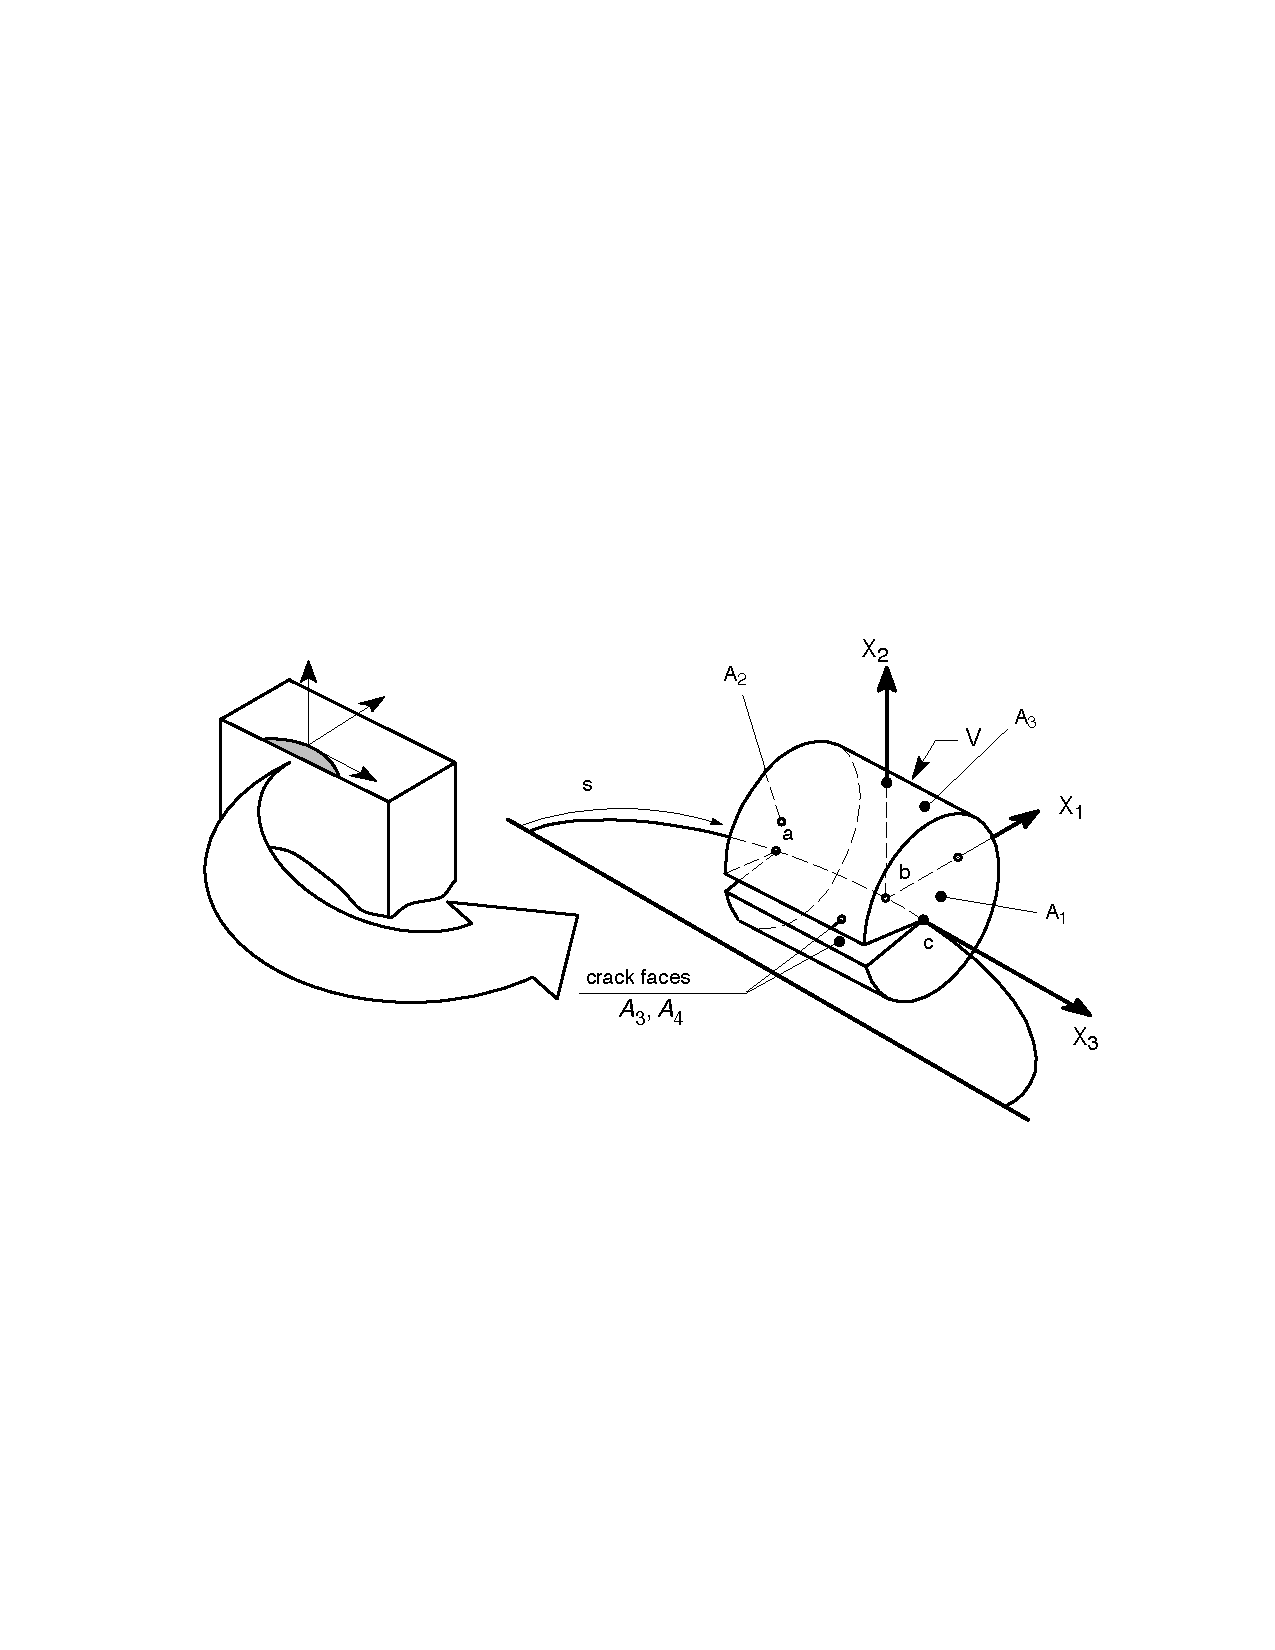
\includegraphics[width=0.8\textwidth]{domain-integral-volume}
\caption[Example of a domain integral volume for numerically calculating \J]{\label{fig:domain-integral-volume} Example of a domain integral volume for numerically calculating \J \citep{warp3d}}
\end{figure}

For a group of elements centered on the (\(x_1, x_2, x_3\)) origin, \J can be calculated as
\begin{align}
J &= \sum_{\substack{\text{all elements}\\\text{in domain}}} \, \sum_{p=1}^{m} 
  \left\{
    \left[
      \left( 
        \sigma_{ij} \pderiv{u_j}{x_1} - w \delta_{1i}
      \right)
      \pderiv{q}{x_i}
    \right]
    \left|
      \pderiv{x_j}{\xi_k}
    \right|
  \right\}
  w_p
\end{align}
with \(w\) equal to the stress work done to an element,
\begin{align}
w &= w^{(\text{e})} + w^{(\text{p})} \\
  &= \Int{\sigma_{ij}}{\epsilon{_{ij}}^{(\text{e})},0,{\epsilon{_{kl}}^{(\text{e})}}} + \Int{S_{ij}}{\epsilon{_{ij}}^{(\text{p})},0,{\epsilon{_{kl}}^{(\text{p})}}}
\end{align}
and a weight function \(q\) that has a value of 1 at the crack tip and 0 along faces \(A_1\), \(A_2\), and \(A_3\) as shown in \Cref{fig:domain-integral-q}, with partial derivatives defined in terms of element shape functions and parametric coordinates as
\begin{figure}[bp]
\centering
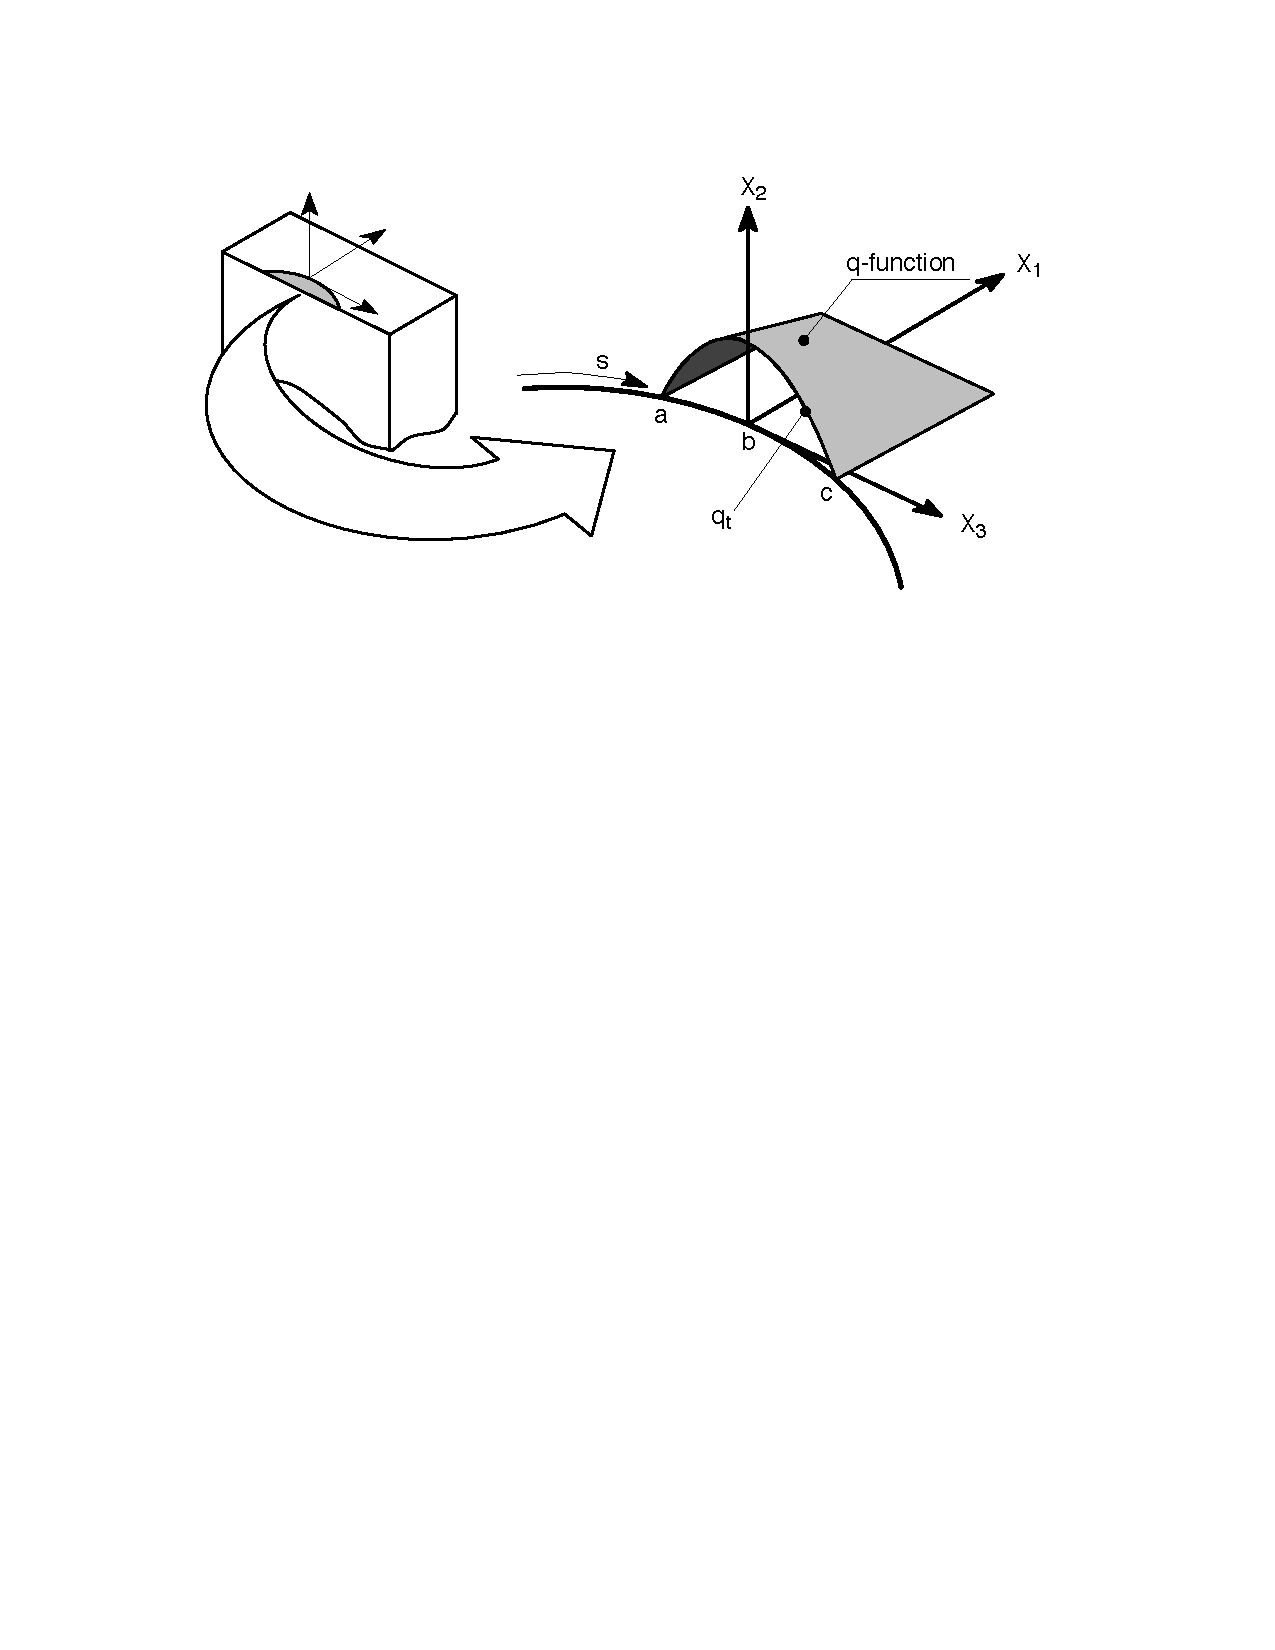
\includegraphics[width=0.8\textwidth]{domain-integral-q}
\caption[\(q\) function for a point along the crack front]{\label{fig:domain-integral-q} \(q\) function for a point along the crack front \citep{warp3d}}
\end{figure}
\begin{align}
\pderiv{q}{x_i} &= \sum_{I=1}^n \sum_{k=1}^{3} \pderiv{N_I}{\xi_k} \pderiv{\xi_k}{x_j} q_I \\
\intertext{where}
m &= \text{number of Gauss points per element} \nonumber \\
w_p &= \text{weight factor at Gauss point } p \nonumber \\
n &= \text{number of nodes per element (in this case, 20)} \nonumber \\
q_I &= \text{nodal value of } q \nonumber \\
N_I &= \text{element shape function} \nonumber \\
\xi_i &= \text{parametric coordinates of element} \nonumber \\
\delta_{ij} &= \text{Kronecker delta} \nonumber \\
S_{ij} &= \text{deviatoric stress tensor.} \nonumber
\end{align}

Though the analytical calculation of \J as a contour integral is path-invariant, the numerical calculation of \J in a finite element model exhibits some path-dependent behavior.
To give the analyst an idea of the accuracy of the calculated \J value, most finite element modeling programs calculate \J using progressively larger volumes of elements seen in \Cref{fig:fem-j-domains}, which should cause \J values to converge to an accurate result.
WARP3D calculates its first domain integral using elements at the crack tip, while Abaqus calculates its first domain integral using the first ring of elements surrounding the crack tip elements.
Both programs calculate additional \J domains by including additional rings of elements surrounding the crack tip, making Abaqus' first \J domain equal to WARP3D's second \J domain.
For the purposes of verification and validation, finite element program developers typically recommend ignoring the first few \J domain values, and using larger domains surrounding the crack tip.
\begin{figure}[tbp]
\centering
\begin{minipage}[b]{0.45\columnwidth}
\setbox1=\hbox{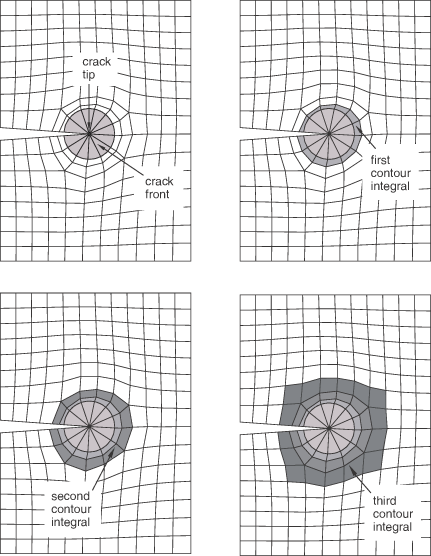
\includegraphics[width=\columnwidth]{contour_integral_regions_abaqus}}
\setbox2=\hbox{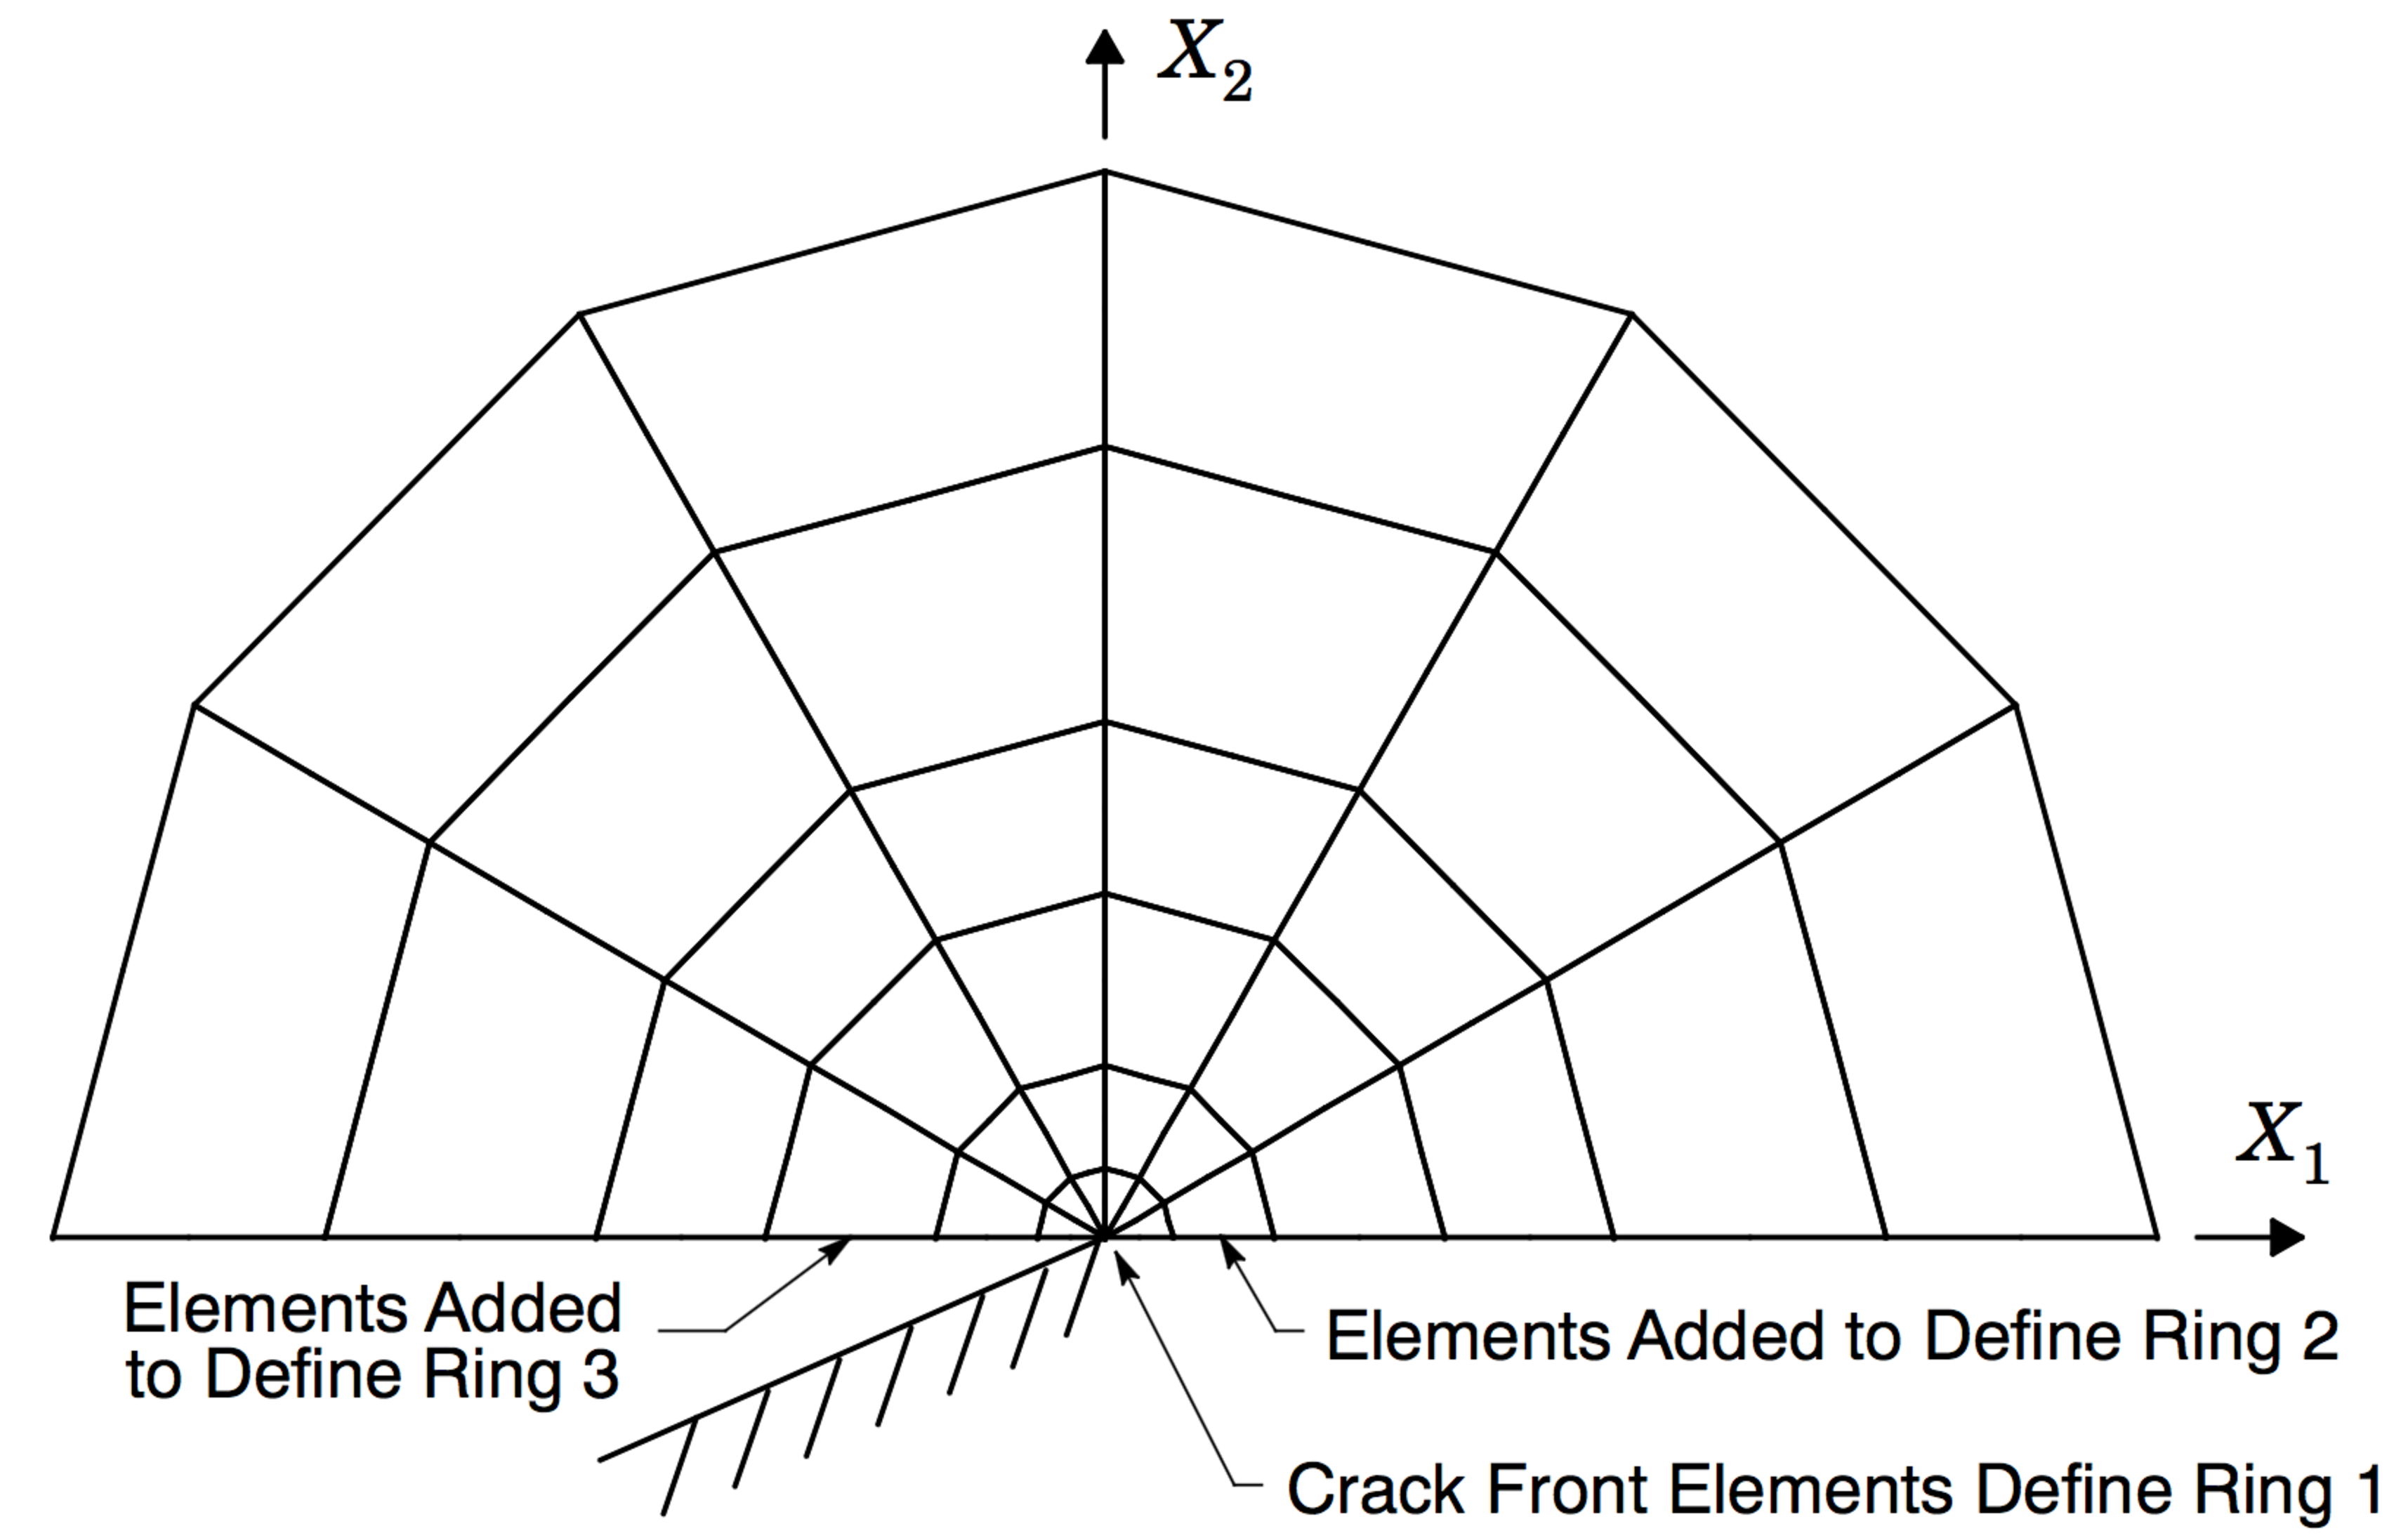
\includegraphics[width=\columnwidth]{contour_integral_regions_warp3d}}
\raisebox{0.5\ht1-0.5\ht2}{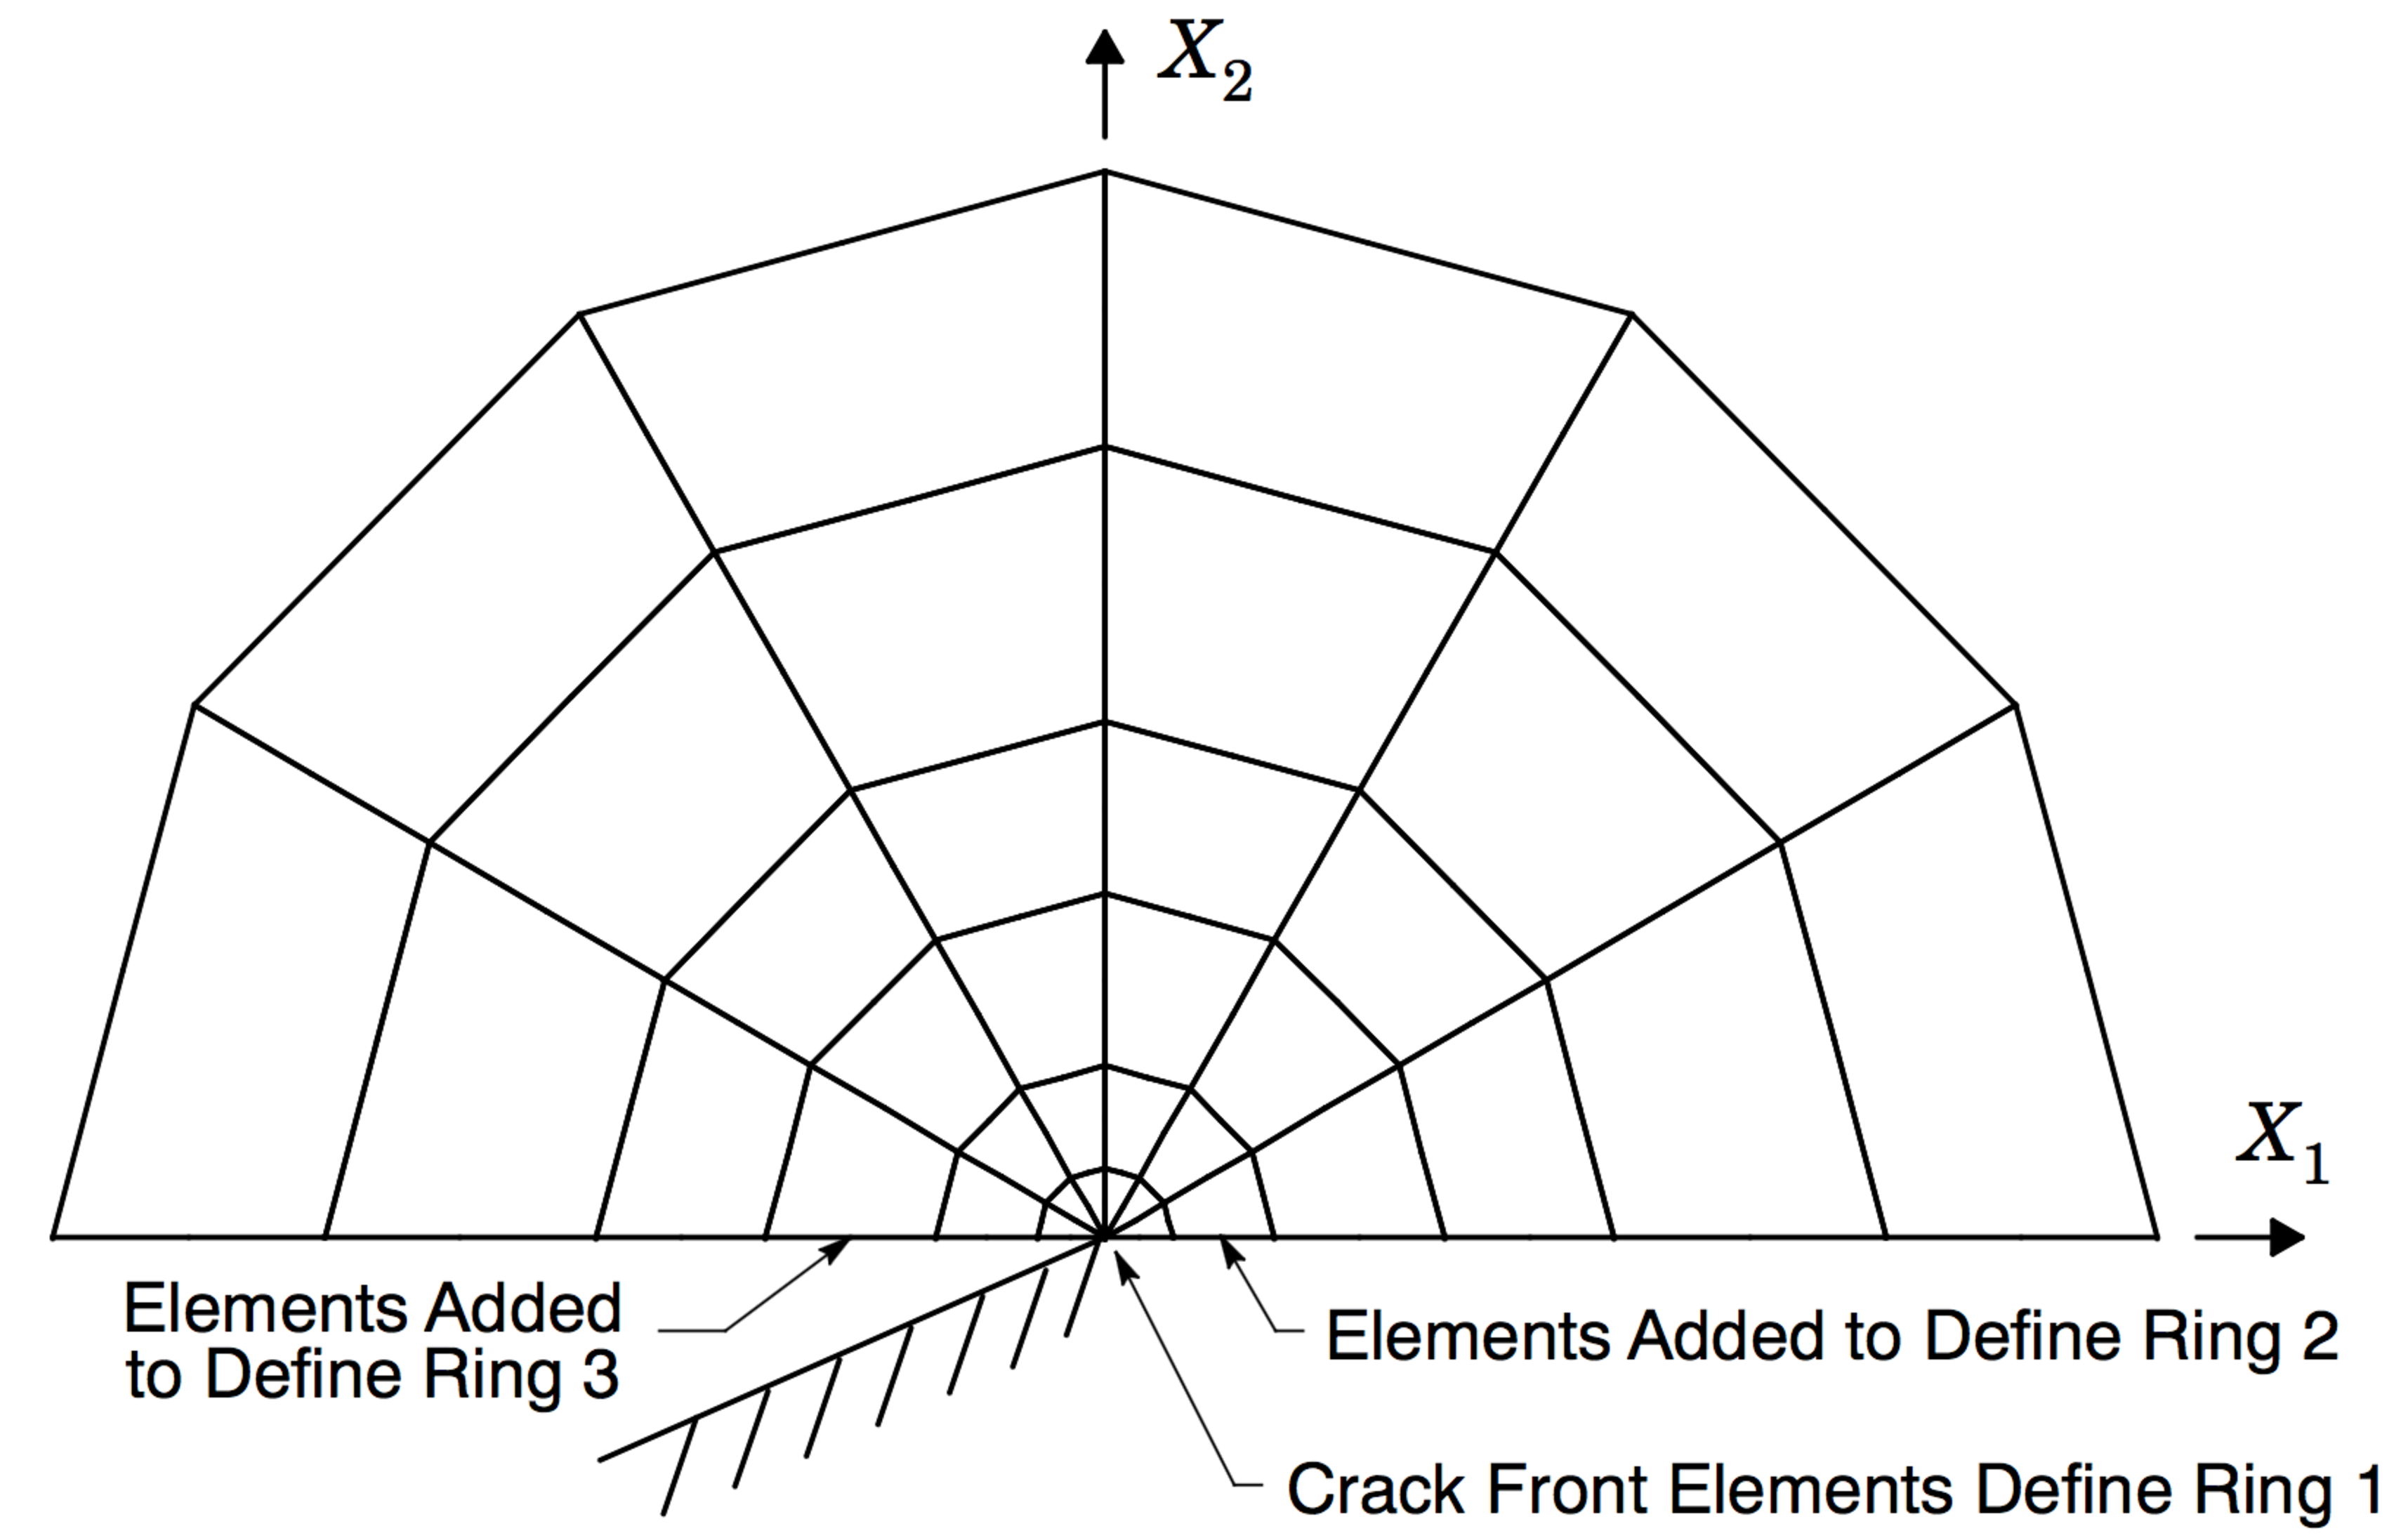
\includegraphics[width=\columnwidth]{contour_integral_regions_warp3d}}
\subcaption{WARP3D}
\end{minipage}
\begin{minipage}[b]{0.45\columnwidth}
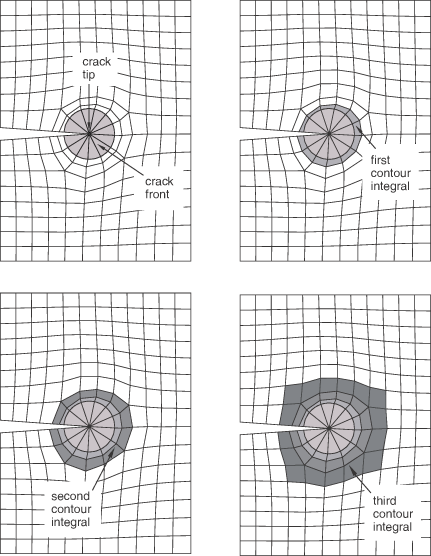
\includegraphics[width=\columnwidth]{contour_integral_regions_abaqus}
\subcaption{Abaqus}
\end{minipage}
\caption{\label{fig:fem-j-domains} Elements used in \J calculations}
\end{figure}

\subsection{Estimation Schemes}
\label{sec:estimation}

Though it is possible to calculate \J using the domain integral method of the previous section, considerable effort would be required to produce finite element models for each geometry and material.
Estimation schemes typically use curve-fitted equations derived from numerical or experimental results, and may include other simplifying assumptions to reduce analytical requirements of calculating \J.

\subsubsection{EPRI Method}
The EPRI technical report ``Engineering Approach for Elastic-Plastic Fracture Analysis'' \citep{epri1981} provided a handbook approach to elastic-plastic fracture mechanics developed for through crack geometries.
The method first assumes that \J is the sum of an elastic component \Jel and a plastic component \Jpl{}.
\begin{align}
\J &= \Jel + \Jpl \label{eq:epri-j}
\end{align}
The elastic component \Jel is defined as in \Cref{eq:j-g}: \(\Jel = \frac{\KI^2}{E'}\).
\KI is calculated using an apparent crack size:
\begin{align}
\aapp &= a_0 + \phi \ry
\intertext{where}
\ry &= \frac{1}{\beta \pi} \left( \frac{n-1}{n+1} \right) \left( \frac{K}{\sigma_0} \right)^2 \\
\beta &=
  \begin{cases}
  2 & \textnormal{for plane stress} \\
  6 & \textnormal{for plane strain}
  \end{cases} \\
\phi &= \frac{1}{1+\left(\frac{P}{P_0}\right)^2} .
\end{align}
The limit load per unit thickness \(P_0\)\nomenclature[1P]{\(P_0\)}{limit load per unit thickness} is calculated from the amount of load required to cause yielding on the net cross section of uncracked material.
For a center-cracked plate loaded in tension:
\begin{align}
P_0 &=
  \begin{cases}
    2 b \sigma_0 & \textnormal{for plane stress} \\
    \frac{4}{\sqrt{3}} b \sigma_0 & \textnormal{for plane strain}
  \end{cases}
\end{align}
where \(b\)\nomenclature[1b]{\(b\)}{uncracked ligament} is the uncracked ligament.
Finally, \Jpl, CMOD, and \(\Delta\) can be calculated as:
\begin{align}
\Jpl &= h_1 \left( \frac{a}{W}, n \right) \left( \frac{P}{P_0} \right)^{n+1} \alpha \epsilon_0 \sigma_0 b \\
\textnormal{CMOD} &= h_2 \left( \frac{a}{W}, n \right) \left( \frac{P}{P_0} \right)^{n} \alpha \epsilon_0 a \\
\Delta &= h_3 \left( \frac{a}{W}, n \right) \left( \frac{P}{P_0} \right)^{n} \alpha \epsilon_0 a \\
\deltat &= \alpha \epsilon_0 b h_4 \left( \frac{a}{W}, n \right) \left( \frac{P}{P_0} \right)^{n+1} \\
       &= d_n \frac{\Jpl}{\sigma_0}
\end{align}
where \hone, \htwo, and \hthree can be found from tables or graphs in \cite{epri1981}.
One such graph is reproduced in \Cref{fig:h1-h2-h3-ccp-plane-strain}.
\hfour is calculated as \(\hfour = d_n \hone\), where \(d_n\) is given in \Cref{fig:dn-plane-strain} for \(\alpha=1\), or
\begin{align}
d_n &= \alpha^{\frac{1}{n}} \left. d_n \right|_{\alpha=1}
\end{align}
for all \(\alpha \neq 1\).
\begin{figure}
\centering
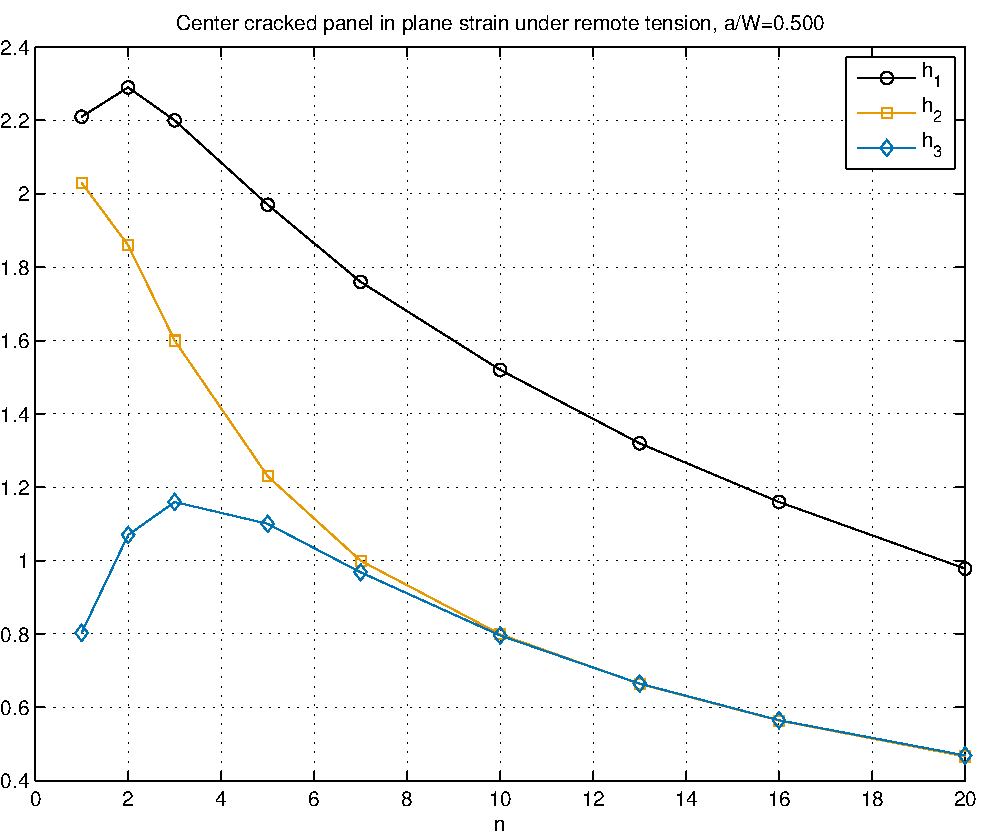
\includegraphics[width=0.8\columnwidth]{h1-h2-h3-ccp-plane-strain}
\caption{\label{fig:h1-h2-h3-ccp-plane-strain} Example EPRI parameters}
\end{figure}
\begin{figure}
\centering
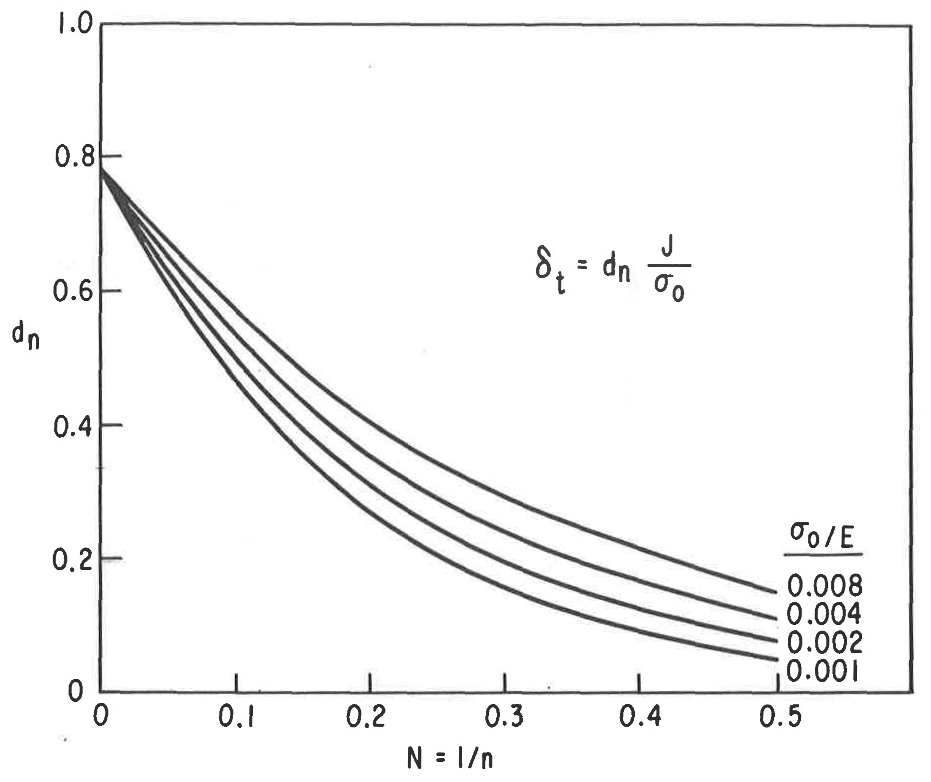
\includegraphics[width=0.8\columnwidth]{dn-plane-strain-modified}
\caption[CTOD parameter for \(\alpha=1\)]{\label{fig:dn-plane-strain} CTOD parameter for \(\alpha=1\) \citep{epri1981}}
\end{figure}

\subsubsection{NASGRO Equation}

The NASGRO suite of fracture mechanics and fatigue crack growth programs \citep{nasgro2000} includes a life assessment program NASFLA for calculating stress intensity factors and crack growth rates for a wide variety of model geometry, material models, and boundary conditions.
Early versions of NASFLA used the Newman-Raju solution for its surface crack growth models.
Later versions include a table of correction factors \(F_\text{p}(\frac{2c}{W}, \frac{a}{c}, \frac{a}{t})\) derived from finite element models for the angles \(\phi = 0\) and \(\phi =\frac{\pi}{2}\).
Selected values of \(F_\text{p}\) are given in \Cref{tab:nasgro-c-tip,tab:nasgro-a-tip}.
The NASGRO stress intensity factor equation is
\begin{align}
\KI &= F_\text{p} \St \sqrt{\frac{\pi a}{Q}} \label{eq:nasgro-ki}
\end{align}
where
\begin{align}
Q &= 1 + 1.464 \left( \frac{a}{c} \right)^{1.65}
\end{align}
is the shape factor of the ellipse representing the crack front.
\begin{table}
\caption[Selected NASGRO stress intensity correction factors $F_\text{p}$ for $\phi=0$]{\label{tab:nasgro-c-tip} Selected NASGRO stress intensity correction factors $F_\text{p}$ for $\phi=0$ \citep{nasgro2000}}
\centering
\begin{tabular}	{ccccccc} \toprule
& & \multicolumn{5}{c}{\(\frac{a}{t}\)} \\ \cmidrule(lr){3-7}
\multicolumn{1}{c}{\(\frac{2c}{W}\)} & \multicolumn{1}{c}{\(\frac{a}{c}\)} & 0.00 & 0.20 & 0.50 & 0.80 & 1.00 \\ \midrule
0.0 & 0.20 & 0.5622 & 0.6110 & 0.7802 & 1.1155 & 1.4436 \\
0.0 & 0.40 & 0.6856 & 0.7817 & 0.9402 & 1.1583 & 1.3383 \\
0.0 & 1.00 & 1.1365 & 1.1595 & 1.2328 & 1.3772 & 1.5145 \\
0.1 & 0.20 & 0.5685 & 0.6133 & 0.7900 & 1.1477 & 1.5014 \\
0.1 & 0.40 & 0.6974 & 0.7824 & 0.9456 & 1.2008 & 1.4256 \\
0.1 & 1.00 & 1.1291 & 1.1544 & 1.2389 & 1.3892 & 1.5273 \\
\vdots & \vdots & \vdots & \vdots & \vdots & \vdots & \vdots \\
1.0 & 1.00 & 1.3956 & 1.8446 & 2.6292 & 3.6964 & 4.5865 \\ \bottomrule
\end{tabular}
\end{table}
\begin{table}
\caption[Selected NASGRO stress intensity correction factors $F_\text{p}$ for $\phi=\frac{\pi}{2}$]{\label{tab:nasgro-a-tip} Selected NASGRO stress intensity correction factors $F_\text{p}$ for $\phi=\frac{\pi}{2}$ \citep{nasgro2000}}
\centering
\begin{tabular}	{ccccccc} \toprule
& & \multicolumn{5}{c}{\(\frac{a}{t}\)} \\ \cmidrule(lr){3-7}
\multicolumn{1}{c}{\(\frac{2c}{W}\)} & \multicolumn{1}{c}{\(\frac{a}{c}\)} & 0.00 & 0.20 & 0.50 & 0.80 & 1.00 \\ \midrule
0.0 & 0.20 & 1.1120 & 1.1445 & 1.4504 & 1.7620 & 1.9729 \\
0.0 & 0.40 & 1.0900 & 1.0945 & 1.2409 & 1.3672 & 1.4404 \\
0.0 & 1.00 & 1.0400 & 1.0400 & 1.0672 & 1.0883 & 1.0800 \\
0.1 & 0.20 & 1.1120 & 1.1452 & 1.4595 & 1.7744 & 1.9847 \\
0.1 & 0.40 & 1.0900 & 1.0950 & 1.2442 & 1.3699 & 1.4409 \\
0.1 & 1.00 & 1.0400 & 1.0260 & 1.0579 & 1.0846 & 1.0820 \\
\vdots & \vdots & \vdots & \vdots & \vdots & \vdots & \vdots \\
1.0 & 1.00 & 1.0400 & 1.2613 & 1.4890 & 1.4558 & 1.3010 \\ \bottomrule
\end{tabular}
\end{table}

\subsection{Load Separation}

\label{sec:intro-load-separation}

\citet{sharobeamlandes1991} reviewed several previous papers as background to their work on calculating \J from a single specimen.
Previously, \J for an edge-cracked plate was defined in terms of an energy rate
\begin{alignat}{2}
\J &=& - \left. \pderiv{U}{A} \right|_{\Delta=\textnormal{constant}} \\
   &=& - \frac{1}{t} \left. \pderiv{U}{a} \right|_{\Delta=\textnormal{constant}}
\end{alignat}
where \(U\) is the strain energy measured as the area under the load-dis\-place\-ment curve, and \(\Delta\)\nomenclature[2\Delta]{\(\Delta\)}{specimen displacement} is a characteristic specimen displacement.
This method required several specimens to determine, since \J was a function of the crack length \(a\).
Recognizing that specimen load was itself a composite function of crack length and material properties, it was reasonable to think that perhaps \J could be separated into geometric and material components.
\citet{riceparismerkle1973} divided \J into elastic and plastic components
\begin{align}
\J &= \Jel + \Jpl .
\end{align}
This form of \J could be rewritten as
\begin{align}
\J &= \etael \frac{A_\textnormal{el}}{b} + \etapl \frac{A_\textnormal{pl}}{b} \label{eq:j-eta}
\end{align}
where
\(A_\textnormal{el}\)\nomenclature[1Ael]{\(A_\textnormal{el}\)}{area under elastic region of load-dis\-place\-ment record} is the area under the elastic region of the load-dis\-place\-ment record, 
\(A_\textnormal{pl}\)\nomenclature[1Apl]{\(A_\textnormal{pl}\)}{area under plastic region of load-dis\-place\-ment record} is the area under the plastic region of the load-dis\-place\-ment record, and both \etael and \etapl are functions of the crack length to specimen width ratio \(\frac{a}{W}\).\nomenclature[2eta]{\(\eta\)}{multiplicative factor for load-dis\-place\-ment record used to calculate \J}
\citet{turner1980} showed that for materials that were not purely elastic or perfectly plastic, a single value of \(\eta\) could be used for the entire specimen record.
Rice estimated \(\eta\) for a center-cracked tension specimen as \(\eta = 1\), and Landes estimated \(\eta = 0.963\) using the load separation method.

If the load can be separated into geometric and material components as
\begin{align}
P &= G \left( \frac{a}{W} \right) H \left( \frac{\Deltapl}{W} \right)
\end{align}	
where \Deltapl \nomenclature[2Deltapl]{\Deltapl}{plastic component of specimen displacement} is the plastic component of a specimen displacement (typically a load-line displacement), then the loads on specimens with different initial crack lengths \(a_i\) and \(a_j\) at a given plastic displacement can be related by a single parameter \(\Sij = \frac{P(a_i)}{P(a_j)}\) as follows:
\begin{align}
\Sij = \left. \frac{P(a_i)}{P(a_j)} \right|_{\Deltapl} &= \left. \frac{P(a_i,\Deltapl)}{P(a_j,\Deltapl)} \right|_{\Deltapl} \\
     &= \frac{G \left( \frac{a_i}{W} \right) H \left( \frac{\Delta_1}{W} \right)}{G \left( \frac{a_i}{W} \right) H \left( \frac{\Delta_1}{W} \right)}
     = \frac{G \left( \frac{a_j}{W} \right) H \left( \frac{\Delta_2}{W} \right)}{G \left( \frac{a_j}{W} \right) H \left( \frac{\Delta_2}{W} \right)} \\
     &= \frac{G \left( \frac{a_i}{W} \right)}{G \left( \frac{a_j}{W} \right)} .
\end{align}
If \Sij\nomenclature[1Sij]{\Sij}{load separation separation parameter} is a constant for the entire range of \Deltapl values examined, then the load \(P\) can be split into separable components. An example of the calculation of \Sij is shown in \Cref{fig:load-separation}.
\begin{figure}
\centering
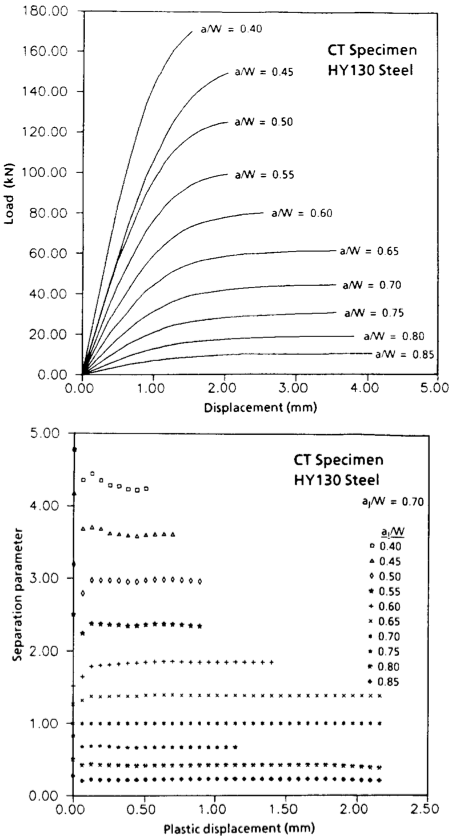
\includegraphics[width=0.6\columnwidth]{load-sep-final}
\caption[Load separation parameter versus plastic displacement for a compact tension specimen]{\label{fig:load-separation} Load separation parameter versus plastic displacement for a compact tension specimen \citep{sharobeamlandes1991}}
\end{figure}
Previous papers have calculated \etapl from \J as
\begin{align}
\J &= - \left| \pderiv{U}{a} \right|_{\Deltapl} = \etapl \frac{A_\textnormal{pl}}{b} \\
\etapl &= \frac{- \left| \pderiv{U}{a} \right|_{\Deltapl}}{\frac{A_\textnormal{pl}}{b}} .
\end{align}
\citet{sharobeamlandes1991} use the separable form of \(P\) and solve for \etapl as
\begin{align}
\etapl &= \frac{G' \left( \frac{a}{W} \right)}{G \left( \frac{a}{W} \right)} \frac{b}{W} \\
G' \left( \frac{a}{W} \right) &= \D{{G\left(\frac{a}{W}\right)}}{\left(\frac{a}{W}\right)} \\
                              &= - \D{{G\left(\frac{b}{W}\right)}}{\left(\frac{b}{W}\right)}
\end{align}
since \(b=W-a\).

Finally, to find \etapl from \Sij, a log-log plot of \Sij against \(\frac{b_i}{W}\) is linear as shown in \Cref{fig:sij-b-w}, indicating that \Sij has a form
\begin{align}
\Sij &= A_1 \left( \frac{b_i}{W} \right)^m \label{eq:sij-b-w} \\
 A_1 &= \left( \frac{b_j}{W} \right)^{-m} .
\end{align}
Similarly, \Cref{eq:sij-b-w} implies that the geometry function \(G(\frac{b_i}{W})\) follows a power law:
\begin{align}
G\left(\frac{b_i}{W}\right) &= A\left( \frac{b_i}{W} \right)^m
\end{align}
and
\begin{align}
\etapl &= \frac{b_i}{W} \frac{m \left(\frac{b_i}{W}\right)^{m-1}}{\left( \frac{b_i}{W} \right)} = m .
\end{align}
\begin{figure}
\centering
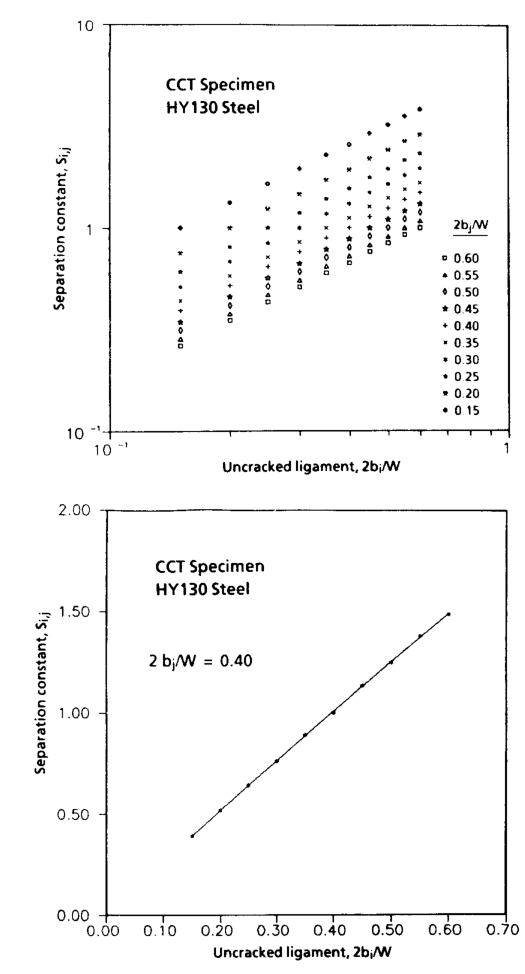
\includegraphics[width=0.55\columnwidth]{load-separation-uncracked-ligament}
\caption[Load separation parameter versus uncracked ligament]{\label{fig:sij-b-w} Load separation parameter versus uncracked ligament \citep{sharobeamlandes1991}}
\end{figure}

Using load separation, \citet{wilsonmani2002} determined \(\etapl\) as a function of the hardening exponent \(n\) as
\begin{align}
\etapl &= 1 - \frac{1}{n}
\intertext{or}
\etapl &= m - \frac{1}{n}
\end{align}
where \(m\) is itself a function of \(n\), and determined that \(m\) varied from 1.022 to 1.069 for plane stress, and from 0.991 to 1.039 for plane strain.

For the surface crack, \citet{sharobeamlandes1994} extended the plastic work factor for through cracks (\etapl) to an equivalent plastic work factor
\begin{align}
\J_{\textnormal{pl,av}} &= \zetapl \int \St d\Delta_{\textnormal{pl,CMOD}} \\
\zetapl &= f\left[ \left( \frac{a}{c}, \frac{a}{t} \right), \textnormal{geometry}, \textnormal{material} \right]
\end{align}
where estimates for \zetapl were found via finite element analysis and load separation. The separation parameter \Sij was written as
\begin{align}
\Sij &= \left[ \frac{\sigma(\frac{a_i}{c_i}, \frac{a_i}{t}, \frac{\Deltapl}{t})}{\St(\frac{a_j}{c_j}, \frac{a_j}{t}, \frac{\Deltapl}{t})} \right]_{\Deltapl}= \frac{G(\frac{a_i}{c_i}, \frac{a_i}{t})}{G(\frac{a_j}{c_j}, \frac{a_j}{t})}
\end{align}
and should be constant for a given material and constraint as shown in \Cref{fig:load-separation-surface-crack}.
\begin{align}
\zetapl &=
  \begin{cases}
  \begin{aligned}
    0.28 +& 0.69 \left( \frac{a}{t} \right) + f_{a,c} + \\
    & \left( 1.835 - 1.67 \left( \frac{a}{t}\right) \right) f_W
  \end{aligned} & 0.1 \leq \frac{a}{t} < 0.5 \\
  0.625 + f_{a,c} + f_W & 0.5 \leq \frac{a}{t} \leq 0.82
\end{cases}
\intertext{where}
f_W &= \frac{t}{W} - 2 \left( \frac{t}{W} \right)^2 \quad (\frac{t}{W}) \leq 0.25, \quad (\frac{c}{W}) \leq 0.25 \\
f_{a,c} &=
  \begin{cases}
  0.22 \left( \sqrt{\frac{a}{t}} - 0.3 \right) \left( \frac{c}{a} -1 \right), & 0.42 \leq \frac{a}{c} \leq 1.0, \frac{a}{t} < 0.5 \\
  0.09 \left( \frac{c}{a} -1 \right), & 0.42 \leq \frac{a}{c} \leq 1.0, \frac{a}{t} \geq 0.5 \\
  -0.08 \left( \frac{a}{c} - 1 \right), & 1.0 \leq \frac{a}{c} \leq 2.0
  \end{cases}
\end{align}
A single-specimen key curve can be constructed by curve-fitting \Sij versus \(\frac{b_e}{t}\), the effective uncracked ligament length from the R6 standard, as shown in \Cref{fig:bet_Sij_original}.
The relationship between the plastic component of CMOD and load line displacement is shown in \Cref{fig:load-separation-cmod-lld-surface-crack}.
Since the two values have a constant ratio over a wide range of \Deltapl values, the equation for \Jpl can be expressed in terms of either measurement.
\begin{figure}
\centering
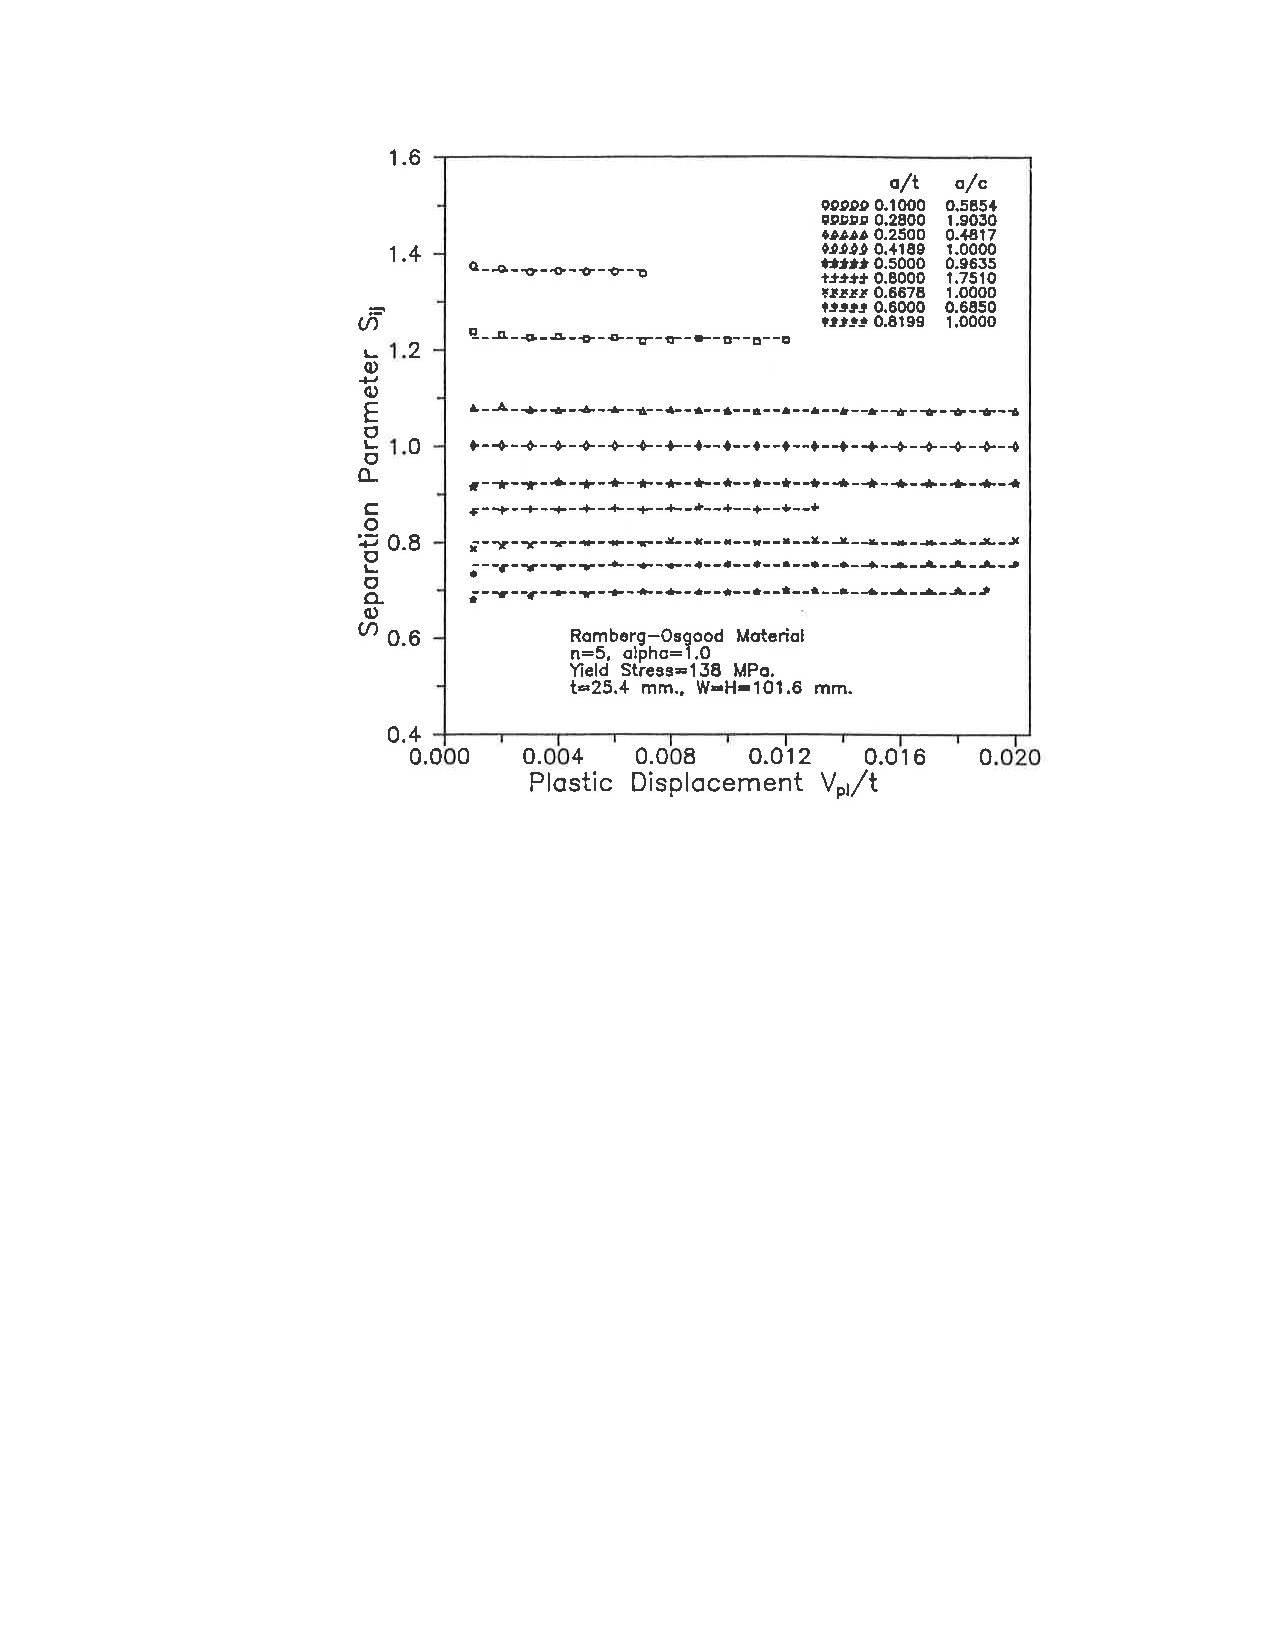
\includegraphics[width=0.6\columnwidth]{load-separation-surface-crack}
\caption[Separation parameter values for surface cracks at various normalized plastic displacements]{\label{fig:load-separation-surface-crack} Separation parameter values for surface cracks at various normalized plastic displacements \cite{sharobeamlandes1994}}
\end{figure}
\begin{figure}
\centering
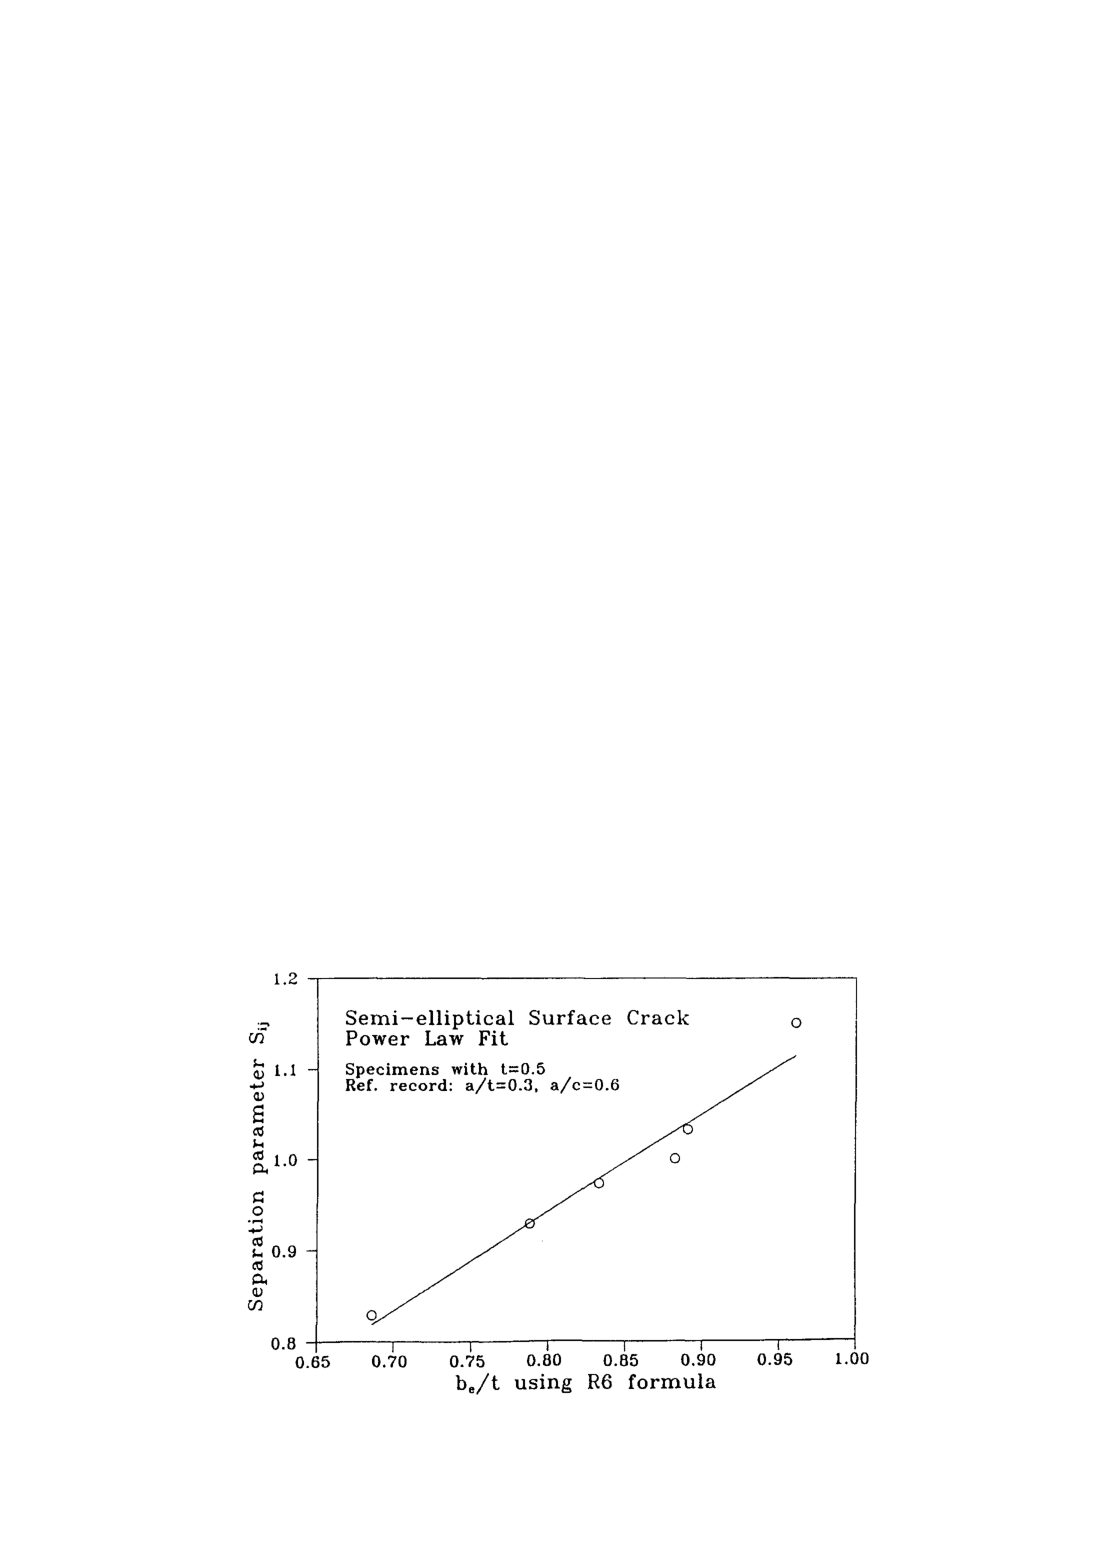
\includegraphics[width=0.6\columnwidth]{bet_Sij_original}
\caption[Separation parameter values versus effective uncracked ligament length]{\label{fig:bet_Sij_original} Separation parameter values versus effective uncracked ligament length \cite{sharobeamlandes1994}}
\end{figure}
\begin{figure}
\centering
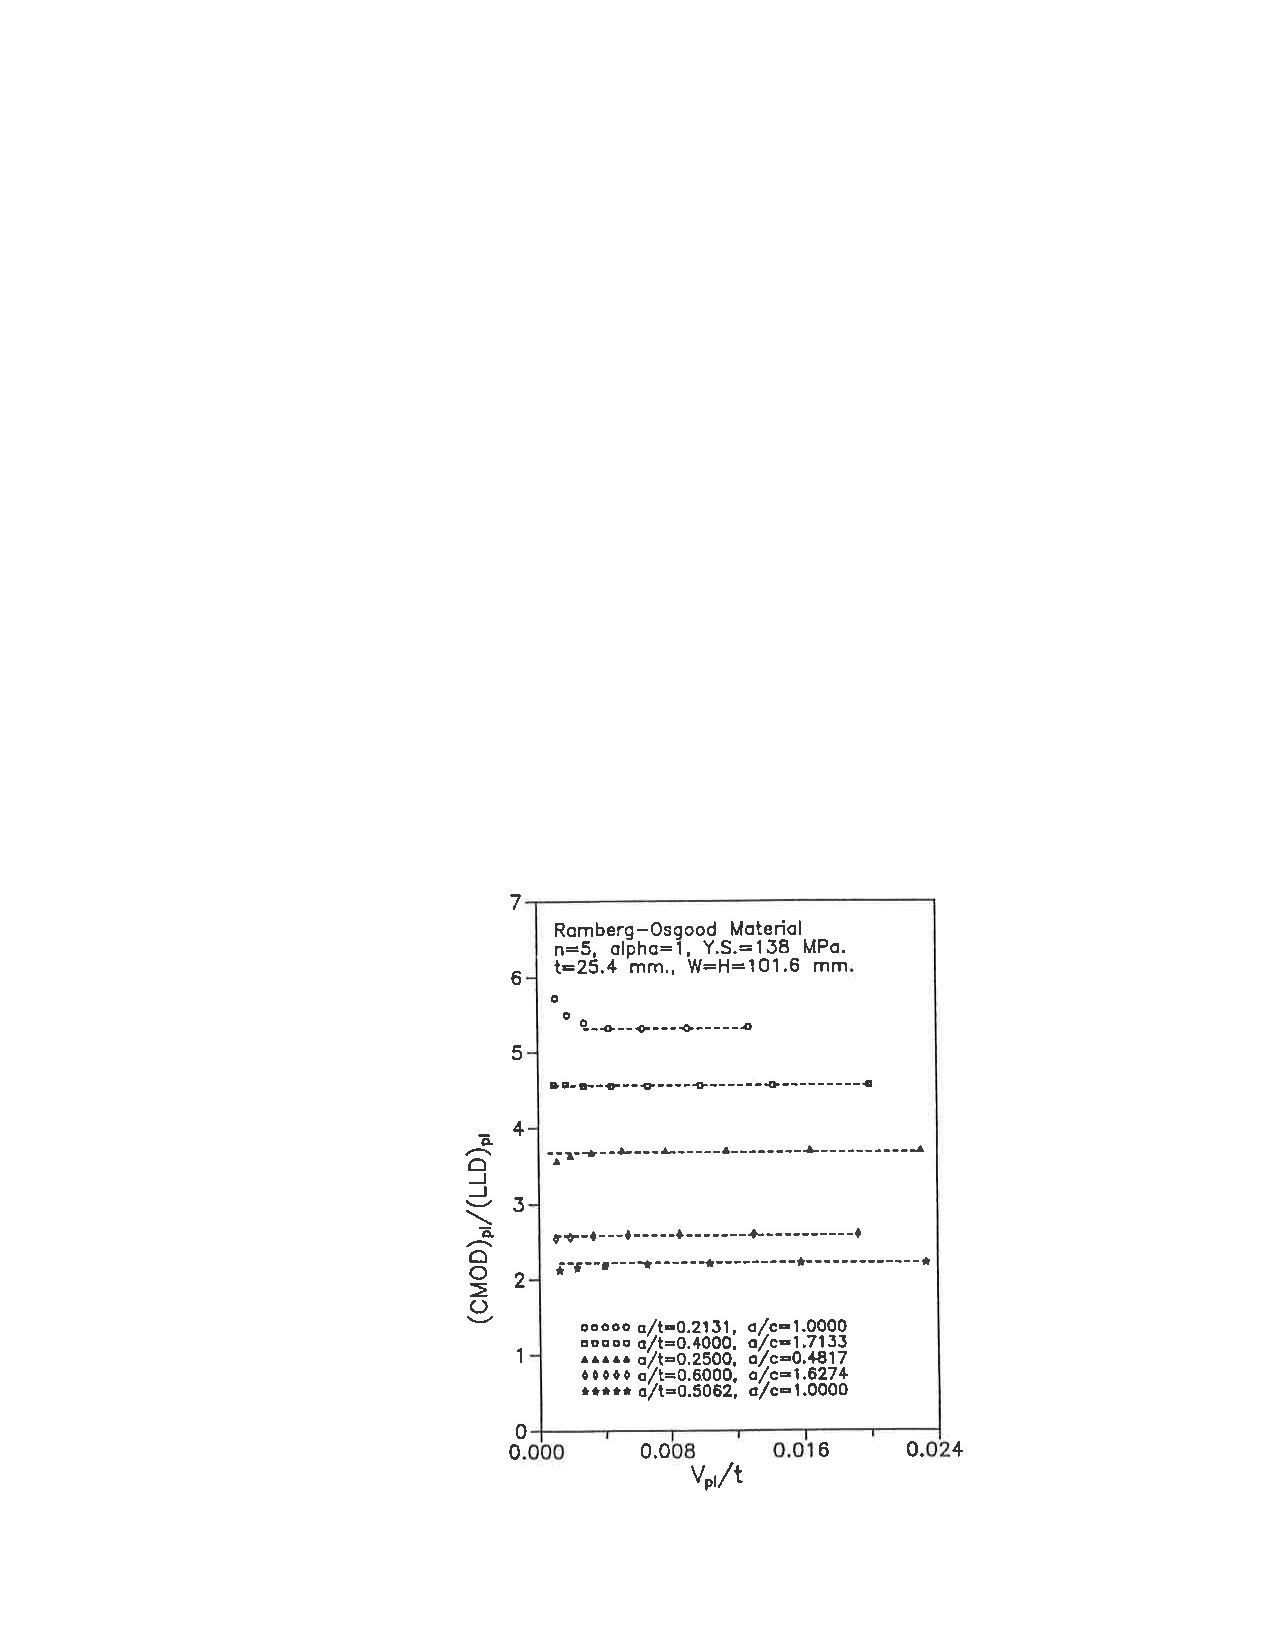
\includegraphics[width=0.6\columnwidth]{load-separation-cmod-lld-surface-crack}
\caption[Relationship between plastic components of CMOD and load line displacement]{\label{fig:load-separation-cmod-lld-surface-crack} Relationship between plastic components of CMOD and load line displacement \cite{sharobeamlandes1994}}
\end{figure}

\FloatBarrier

\section{Engineering Approaches for Elastic-Plastic and Fully-Plastic Analysis of Surface-Cracked Plates in Bending}

This section will give an overview of ASTM E2899, methods for satisfying its analysis requirements to ensure the validity of experiments, and the limitations of the TASC software tool often used for that analysis.

\subsection{ASTM E2899}

In ASTM E2899 \cite{astme2899}, a semi-elliptical surface starter crack is machined into a flat rectangular plate, and the starter crack is fatigued to induce a sharper crack front.
After the initial fatigue cycles have completed, the plate is subjected to monotonically increasing bending or tension force while the CMOD is monitored.
As the force is applied, either the specimen will fail due to unstable crack growth, or else the initiation of stable crack tearing is detected via methods including electric potential drop, measurement of CMOD, monitoring acoustic emissions, or crack shape replicates.
Once crack growth has been detected, the angular position where crack growth occurs (\(\phi_i\)) is recorded, and material properties and crack-front conditions are used to identify which of the linear elastic, elastic-plastic, or fully-plastic (field collapse) regimes are applicable to the specimen and loading condition.
If either the linear elastic or elastic-plastic regimes are applicable, constraint measures at \(\phi_i\) are calculated from tables, and if the constraint value is negative, both the constraint and the value of \K at \(\phi_i\) (for linear elastic) or \J at \(\phi_i\) (for elastic-plastic) is reported.
If the constraint value is positive, only \K or \J is reported.
For the linear elastic regime, Annex A1 of ASTM E2899 provides a series of 19 equations that provide accurate estimations of \KI for \(\frac{a}{c} \leq 1\) and \(\frac{a}{t} \leq 0.8\).
No such set of equations exists for the elastic-plastic regime, thus other methods must be employed to calculate \J.
Annex A6 of ASTM E2899-15 recommends finite element analysis using domain integrals to calculate \J.

The analysis requirements of ASTM E2899 go far beyond earlier standards for measuring fracture toughness.
As seen in \Cref{tab:astm-analysis-requirements},
\begin{table}[tbp]
\caption{\label{tab:astm-analysis-requirements} Analysis Requirements in Several ASTM Standards}
\begin{tabular}{c p{0.5\textwidth} p{0.3\textwidth}} \toprule
 & Requirements & Tools \\ \midrule
E8 & Fit linear region of stress-strain curve, offset to find yield strength & Strip chart and calculator \\
E399 & Fit linear region of force-CMOD curve, draw secant line with 5\% less slope, calculate \K with algebraic equations & Strip chart and calculator or spreadsheet \\ 
E740 & Calculate \K with algebraic equations at two positions, report higher value & Calculator or spreadsheet \\
E1820 & Calculate \K with algebraic equations. EPRI method with \Jel calculated from \K and \Jpl calculated from area under load-displacement curve and algebraic equations & Spreadsheet \\ \bottomrule
\end{tabular}
\end{table}
earlier standards can be completed with pocket calculators or simple spreadsheets, tools that are well within reach of any engineer or test facility, and the calculations are easily verified and checked by others.
Only ASTM E2899 requires an elastic-plastic finite element analysis to calculate \J.
Not only is the software used to perform this analysis much more expensive than a spreadsheet or calculator, it requires a much higher level of skill to create an accurate analysis, and is much more difficult for others to verify and check the results.

\subsection{Interpolation}

Performing a finite element analysis for every crack geometry and set of material properties would prove to be quite time-intensive.
It is reasonable to assume that the variation in experimental results from theoretically identical specimens is large enough to allow interpolated results derived from similar geometry and material properties to fall within the range of experimental error.
In that case, the need to perform finite element analysis on every model can be replaced by performing finite element analysis on enough models spanning a range of typical crack geometries and material properties.

\subsection{Tool for Analysis of Surface Cracks (TASC)}

NASA Marshall Space Flight Center (MSFC) has developed a MATLAB program, Tool for Analysis of Surface Cracks (TASC) \citep{allenwells2014, tasc}, to interpolate \J values and surface crack nucleation conditions for a wide range of crack geometries and materials loaded purely in tension.
The development of TASC required the solution of 600 finite element models for geometries spanning
 (\(0.2 \leq \frac{a}{c} \leq 1.0,\; 0.2 \leq \frac{a}{t} \leq 0.8\)) and materials spanning (\(100 \leq \frac{E}{S_{\text{ys}}} \leq 1000,\; 3 \leq n \leq 20\)) shown in \Cref{fig:tasc-geometries,fig:tasc-materials}.
\begin{figure}
\centering
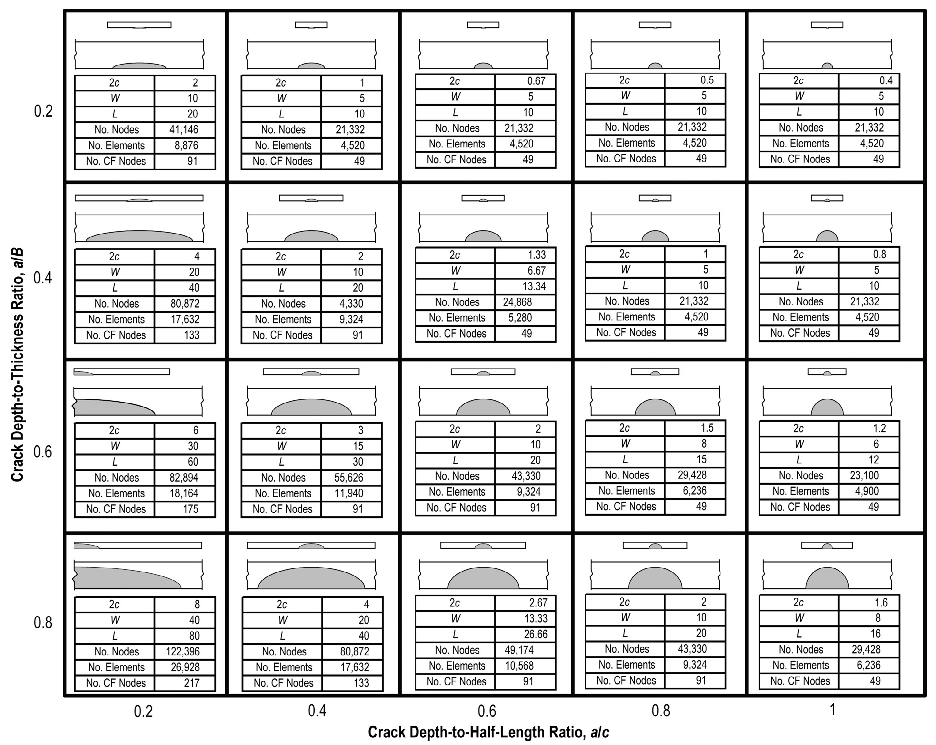
\includegraphics[width=\textwidth]{tasc-geometries}
\caption[Crack geometries used in TASC]{\label{fig:tasc-geometries} Crack geometries used in TASC \citep{allenwells2014}}
\end{figure}
\begin{figure}
\centering
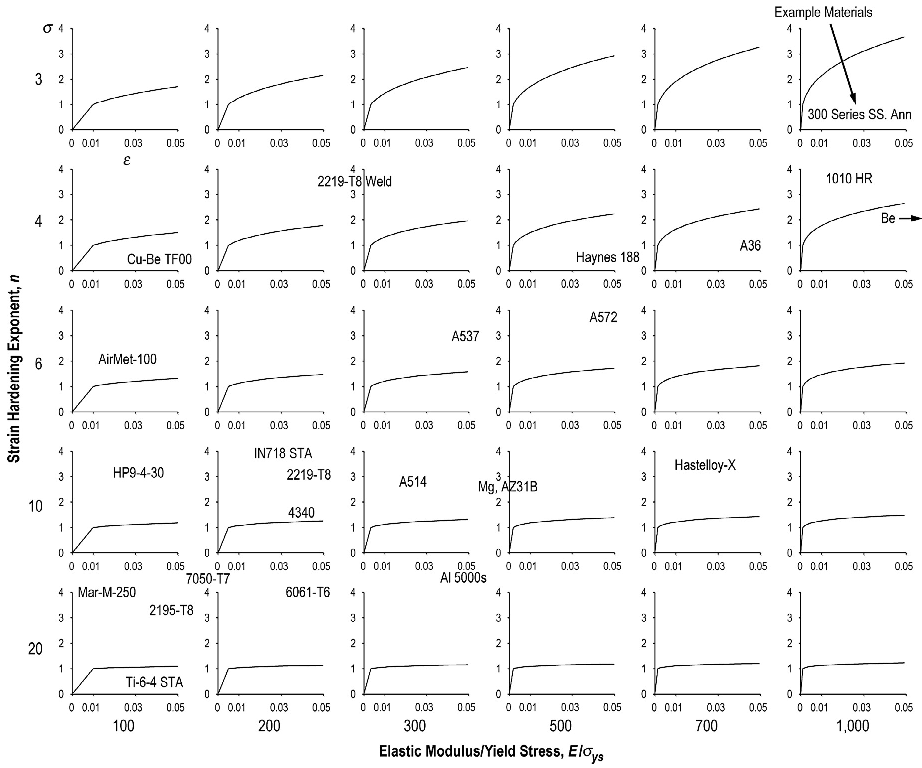
\includegraphics[width=\textwidth]{tasc-materials}
\caption[Material models used in TASC]{\label{fig:tasc-materials} Material models used in TASC \citep{allenwells2014}}
\end{figure}
Results for each model were condensed to a normalized \J as a function of a normalized CMOD and \(\phi\), and the normalized CMOD in terms of a normalized far-field stress as shown in \Cref{fig:tasc-sample-result}.
\begin{figure}
\centering
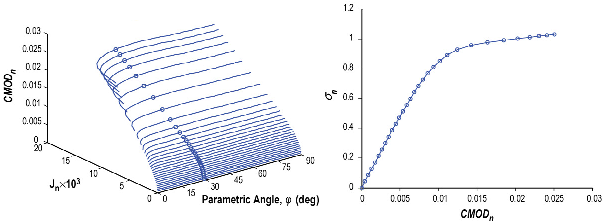
\includegraphics[width=\textwidth]{tasc-sample-result}
\caption[Sample result used by TASC for interpolations]{\label{fig:tasc-sample-result} Sample result used by TASC for interpolations \citep{allenwells2014}}
\end{figure}
TASC uses normalized geometries and material properties, interpolates intermediate results for any geometry and material property spanned by its database, and then scales the interpolated results back to the true physical parameters of an experiment or model.
As TASC does not currently include support for bending loads, MSFC has expressed interest in extending the TASC code and results database to include bending.
Bending conditions introduce additional complexity to the boundary conditions and crack tip constraint, and will need some additional steps taken to ensure accurate results.
These steps are outlined in the next section.
\FloatBarrier
\section{Verification and Validation}
It is apparent throughout the preceding sections that both analytical and experimental techniques for predicting conditions at a crack front include inherent uncertainty.
Even worse, applying the wrong techniques (for example, using an elastic material model when significant plastic deformation is present) can lead to outright errors.
Deviations between predicted behavior and measured behavior can be attributed to two main causes:
repeatability and accuracy of measurements or calculations,
and
application of the correct models or experimental procedures to include all significant physical effects.
Addressing and correcting issues with repeatability and accuracy is improving verification,
and
addressing and correcting issues with application of models or procedures to include all significant effects is improving validation.%

The U.S. Department of Defense Standard MIL-STD-3022 ``Documentation of Verification, Validation, and Accreditation (VV\&A) for Models and Simulations'' (\citeyear{mil-std-3022}) defines validation as ``the process of determining the degree to which a model, simulation, \ldots{} and their associated data are accurate representations of the real world'', and verification as ``the process of determining that a model, simulation, \ldots{} and their associated data accurately represents the developer's conceptual description and specifications''.
In the domain of software engineering, \citet{boehm1989} summarized validation as part of ``building the right product'' and verification as part of ``building the product right''.

The American Society of Mechanical Engineers ``Guide for Verification and Validation in Computational Solid Mechanics'' (\citeyear{asme-vv}) defines the goal of V\&V as validating a model for its intended use.
In this application, demonstrations of both the model's predictive capability and accuracy are required.
Defining the model's intended use also imposes a set of limitations on the applicability of the model.
An example given is predicting the response of a specific make and model of vehicle to frontal impacts against a rigid wall.
Validation requirements may include predicting the compaction of the front end of the vehicle within 20\% accuracy versus experiments run at 10, 20, and 30~mph.
If a model passes the validation tests, it can be assumed to be useful in predicting compaction at any speed up to 30~mph, but this does not ensure any accuracy for crashes at higher speeds, in different directions, on different frames, or against items other than rigid walls.

Real-world physical systems are often composed of several assemblies.
Each assembly includes multiple subassemblies, and each subassembly is a collection of individual components.
Similarly, a system-level model can be constructed from several assembly models, each of which includes subassembly and component models.
Inaccuracies in lower-level models are typically compounded in higher-level models, which means that a given level of accuracy at the system level requires higher accuracy for subassembly and component models.
For example, a model that calculates the buckling strength of a tubular steel strut to 10\% accuracy may mean the accuracy of a model that calculates the collapse strength of a frame made from the struts to 20\% accuracy.

It should be noted that practical computational limits require simplification of lower-level models when higher-level models are created.
Modeling every component of a complex system to maximum accuracy would make a system-level model that would take a huge amount of time and resources to solve.
For example, a finite element model of a tubular steel strut may use two-dimensional shell elements or three-dimensional solid elements, but the response of the strut can be simplified to a model using one-dimensional (possibly nonlinear) beam elements.
Additional error in higher-level models is due to these simplifications, and also to interaction between components that may be difficult to predict in advance.

\subsection{Model Development}

In ASME V\&V procedures, model development is composed of four tasks:
\begin{enumerate}
\item formulation of conceptual models,
\item converting the conceptual model to a computational model,
\item revising models during V\&V,
and 
\item quantifying sensitivity and uncertainty of parameters in the model.
\end{enumerate}
Model development assumes that the physical system of interest, use of the model, and accuracy requirements have been previously defined.

Development of the conceptual model includes defining fundamental assumptions such as
how many components will be included in the model (fasteners, electronics),
models of material behavior (elastic, elastic-plastic, temperature dependent),
elimination of unimportant geometric features (external rounds, small holes in areas of low stress),
and
selection of boundary conditions (fixed, pinned, free) and component interfaces (bonded, frictionless, frictional).
Inadvertent elimination of important mechanical phenomena may lead to inadequate simulations, while focusing on essential physical processes ensures the model solves quickly and accurately.
Development of conceptual models requires defining response features of interest: the characteristics of the physical system that need to be accurately predicted for the model's intended use.
Constructing a Phenomena Identification and Ranking Table (PIRT) is a common tool in identifying key physical characteristics required for accurate simulation.
The PIRT is normally constructed by a group of subject experts who rank physical processes according to their influence on the response characteristics.
An example of a PIRT is given in \Cref{tab:pirt}.
An additional use of the PIRT is in ranking which phenomena require additional scrutiny during the validation phase: in the example PIRT, validating plasticity may be less important if prior experience indicates that it can be modeled with high confidence.
Fracture may be less important to validate if it has little influence on the response of interest.
On the other hand, interface and loads have a greater influence and less confidence, and would be the focus of validation activities.
\begin{table}[bp]
\caption[PIRT example]{\label{tab:pirt} PIRT example \citep{asme-vv}}
\centering
\begin{tabular}{cccc} \toprule
           &            & Importance to & Level of \\
           & Type of    & Response of   & Confidence \\
Phenomenon & Phenomenon & Interest      & in Model \\ \midrule

A & Interface & High & Medium \\
B & Plasticity & Medium & High \\
C & Loads & Medium & Low \\
D & Fracture & Low & Low \\ \bottomrule
\end{tabular}
\end{table}

Development of computational models starts with converting the assumptions and phenomena in the conceptual model into equations and other mathematical statements.
Specification of the mathematical model also helps define responses in terms of model input parameters, such as loads, material properties, and coefficients of friction.
Once the mathematical model has been defined, it can be converted into a computational model.
The computational model is a numerical implementation that approximates the mathematical model, and can include procedures for spatial and temporal discretization, solution of systems of governing equations, and convergence criteria for iterative solution methods.
The computational model can use an existing simulation code, or one written specifically for the current model.
The model can be as simple or complex as necessary.
The analyst responsible for the computational model must understand the assumptions made during the earlier stages, and the influence of parameters and boundary conditions on the model's results: for example, the influence of end conditions on a buckling problem.

There are two primary causes for model revision: to meet accuracy requirements, or to meet previously-unknown requirements.
There are two general methods for revising the model: adjustment of model parameters, or modifying the form of the model and governing equations.
Updates to model parameters are a method to adjust for common sources of modeling difficulty, such as compliance in joints, energy loss or damping, and uncertainty in boundary conditions.
Parameters are adjusted to bring the model responses closer to experimental values.
However, adjustment of parameters to exactly fit one experiment may inadvertently create worse fits with future experiments.
If parameters can be measured independently, those measurements should drive parameter adjustment.
Modifying the form of the model requires changing the mathematical model (and thus, the computational model).
It is most commonly performed when reasonable experimental uncertainty in parameters cannot account for differences in responses, or when observations of physical behavior in an experiment do not match model assumptions (for example, if assumed planar motion has a significant out-of-plane component, if supports assumed to be rigid show significant compliance, if surfaces assumed to be in constant contact separate from each other, etc.).

Performing a sensitivity analysis of the computational model can highlight previously-unknown phenomena: for example, does reducing the wall thickness slightly cause buckling effects to appear?
It can also point out the relative significance of various model parameters.
Information gathered in the sensitivity study can modify the PIRT, increasing or decreasing the importance of parameters.
Sensitivity analysis should be performed after each model revision, since small changes in the model can cause major changes in responses.

Though uncertainty is obviously a part of an experimental program, it is also present in simulations.
Uncertainties at any stage of development can be broadly classified as aleatory (or irreducible) and epistemic (or reducible).
Aleatory uncertainties are inherent in physical systems, and have root causes in the variation of physical properties and processes.
No manufactured component is free from geometric deviations, no material property has exact textbook values in every specimen, and no assembly is constructed with exact fastener preloading, alignment, etc.
Though this uncertainty can never be eliminated, it can be quantified by conducting tests to establish statistical characteristics for each parameter (mean, variance, distribution type).
Once the uncertainty in parameters is quantified, their variability can be propagated through simulations with probabilistic analysis, setting lower bounds on how much variability will be present in the simulation results.

Epistemic uncertainties are the result of incomplete information or knowledge.
Two major categories of reducible uncertainties are statistical uncertainty and modeling uncertainty.
Statistical uncertainty occurs whenever a limited number of samples is used to establish statistical material properties: if only two or three tests are performed, estimates on the population mean and variance will be much worse than if 30 tests are performed.
Modeling uncertainty can be difficult to quantify, but it derives from assumptions made during modeling.
If a material property is assumed to be constant for the simulation, but in reality is time-dependent, temperature-dependent or otherwise variable, the assumption of constant properties is a source of reducible uncertainty.

\subsection{Verification}

Verification is the process of comparing the computational model to the original mathematical model.
It precedes validation, and examines the computational model in the contexts of numerical analysis, software quality engineering, identification of programming errors, and numerical error estimation.
Verification is divided into two main task areas: code verification and calculation verification.

Code verification is composed of two groups: numerical code verification and software quality engineering (SQE).
Numerical code verification verifies that the solution algorithms are correctly programmed.
This often involves convergence testing with different discretization levels and comparison to known analytical solutions.
Software quality engineering procedures seek to eliminate flaws in both the solution code, and in any underlying libraries, compilers, processors, or other tools used in the calculation.

Calculation verification often builds on convergence studies from the code verification stage, and uses numerical solutions from two different models to determine the influence of mesh size and mesh bias.
Methods normally use either gradient tests or analysis of residuals as either the mesh size or the order of the finite elements change.
One area where calculation verification has problems is around discontinuities or singularities (such as the stress field at a crack tip).

\subsection{Validation}

The goal of validation activities is to assess the model's predictive capability by comparing numerical results to corresponding experimental results.
Proper comparison of results can only occur after the following criteria are satisfied:
\begin{itemize}
\item defining the model's intended use,
\item conclusion of code verification and calculation verification, and
\item quantifying uncertainties in both the numerical and experimental results.
\end{itemize}
The validation experiments must be distinct from any earlier experiments used in the verification stage.
The goal is to design and conduct a set of experiments providing a stringent enough test of the model to establish its predictive capability.
If the model predicts the results of all the validation experiments to the predefined level of accuracy, it is assumed to be validated for its intended use.

\subsection{V\&V Efforts within the Fracture Mechanics Community}

V\&V has been applied in the study of fracture mechanics and fatigue life prediction.
\citet{favanesi1994} performed V\&V activities on the NASCRAC fracture mechanics software, verifying it against the FLAGRO and FRANC2D codes, and also validating it against \citet{tadaparisirwin1973} or their own experimental tests.
The most basic predictions (\K versus \(a\), \J versus \(a\)) were generally verified and validated, but other predictions (proof tests, creep, crack retardation) were either invalid, or the uncertainty in experimental measurements was high enough to make results inconclusive.
\citet{wilson1995} identified problems with both NASCRAC and FLAGRO.
NASCRAC contained two types of errors in its material database: both were related to assuming that certain fracture properties (\Kc and \(m\)) were constant instead of functions of geometry and load.
NASCRAC also showed significant deviations from previously-established fatigue crack growth curves, well beyond the limits of uncertainty, as shown in \Cref{fig:nascrac-vv-tension}.
\begin{figure}
\centering
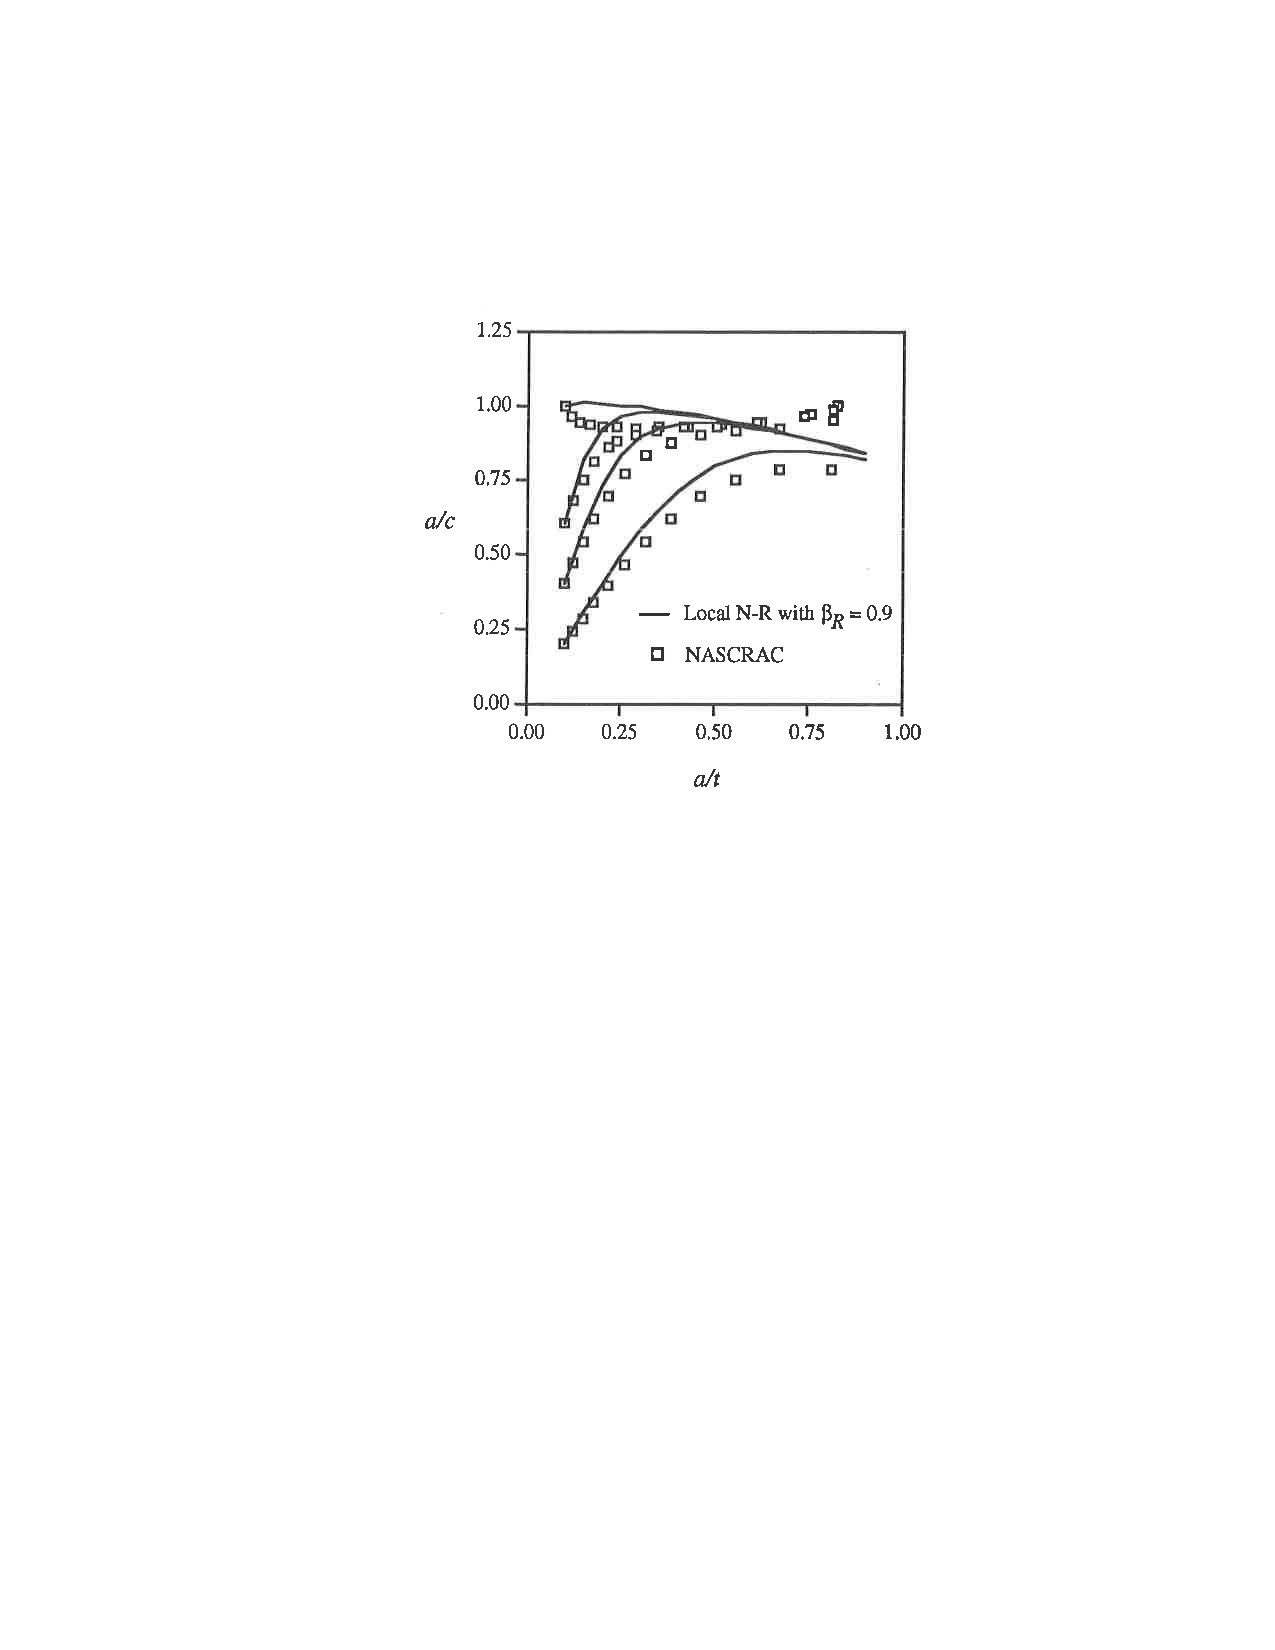
\includegraphics[width=0.5\columnwidth]{nascrac-vv-tension}
\caption[Comparison between NASCRAC fatigue crack growth curves and previous results]{\label{fig:nascrac-vv-tension} Comparison between NASCRAC fatigue crack growth curves and previous results \citep{wilson1995}}
\end{figure}
The FLAGRO source code, written in FORTRAN, contained several instances of non-portable statements, non-standard use of \verb|COMMON| blocks, and little use of program flow control (\verb|IF/THEN/ELSE| statements).
\citet{mcclung2012} outlines the V\&V process in great detail, and shows an example of verifying a \K solution by comparing the FADD3D, FEACrack, and FLAGRO solvers.
All three were in good agreement through most of the crack front, but FEACrack deviated from the others at \(\phi=0\) and \(\phi=\pi\).
McClung also showed the large amounts of work remaining to complete the V\&V process on fracture mechanics.

The next chapter will build on existing techniques from this chapter, including EPRI estimation, load separation, models used for the TASC database, interpolation, and V\&V to verify results from the literature.
The verification work done will be used to improve the quality of the work required for the current research. 

\chapter{Modeling Preparation for Research Tasks}
\label{chap:verification-tensile-sc}
As the primary goal of this research is to develop a database of elastic-plastic finite element models and results for flat plates in bending, the programs and techniques used to create that database can be validated against existing tension cases.
These techniques are first applied to models used for EPRI \hone calculations, then to a group of models demonstrating load separation, and finally to two models from the existing TASC program leading to an interpolated result for an intermediate material.

\section{EPRI \hone Verification}
\label{sec:h1-verification}

The finite element method used in the EPRI report \citep{epri1981} was extended to fully-plastic \J solutions for three-dimensional geometries in \citet{mcclung1999}.
ABAQUS was used for the elastic-plastic analysis using an incremental plasticity model.
\Cref{fig:geometries} shows the models examined for \(n=5, 10, \textnormal{ and } 15\).
Once values for \Jpl were calculated, \hone values comparable to the EPRI graphs were calculated as
\begin{align}
\hone &= \frac{\Jpl}{\alpha \sigma_0 \epsilon_0 t \left( \frac{\sigma}{\sigma_0}\right)^{n+1}} \label{eq:h1mcclung}
\end{align}
using a Ramberg-Osgood power-law material model.
\citet{lei2004} ran both elastic and elastic-plastic models for the same geometries with \(n=5\) and \(n=10\).
\citet{quillen2005} ran both elastic-plastic and fully-plastic models with various mesh densities, element types, and material models.
Each of Quillen's Abaqus models had some anomalies in the \hone values compared to McClung and Lei at the free surface, the symmetry plane, and at the third node from the free surface.
Values at each of these positions was higher than the trend exhibited by neighboring points.
Some models displayed small discrepancies, others were quite large.
At the time, no reason was identified for the anomalies. \Cref{fig:model3_n10_2005,fig:model5_n5_2005} show two such sets of discrepancies.

\begin{figure}[tbp]
    \centering
    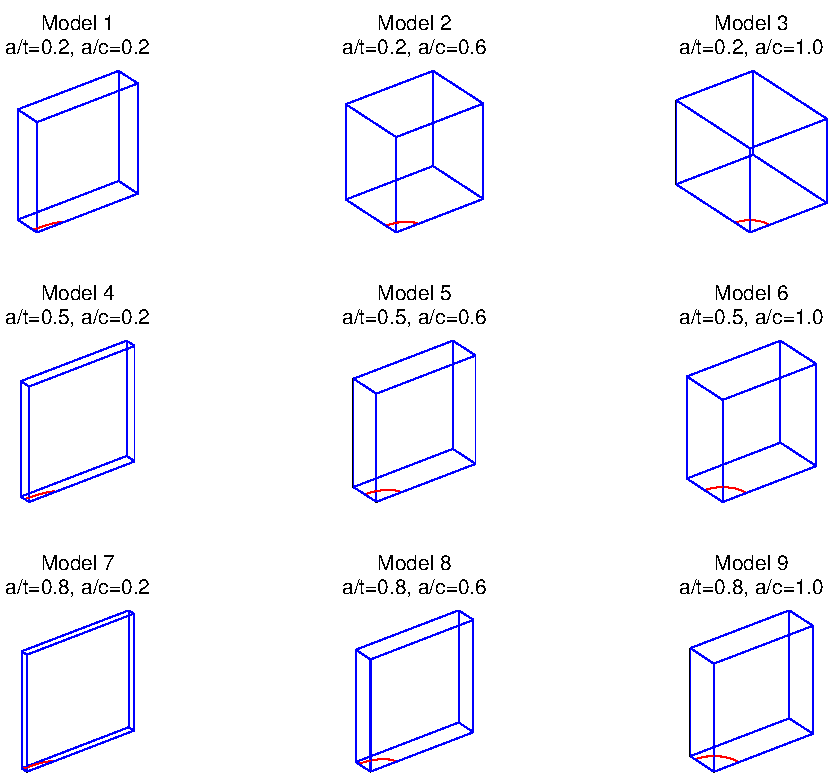
\includegraphics[width=0.8\columnwidth]{geometries}
    \caption{McClung et al. model geometry \label{fig:geometries}}
\end{figure}

\begin{figure}[tbp]
  \centering
  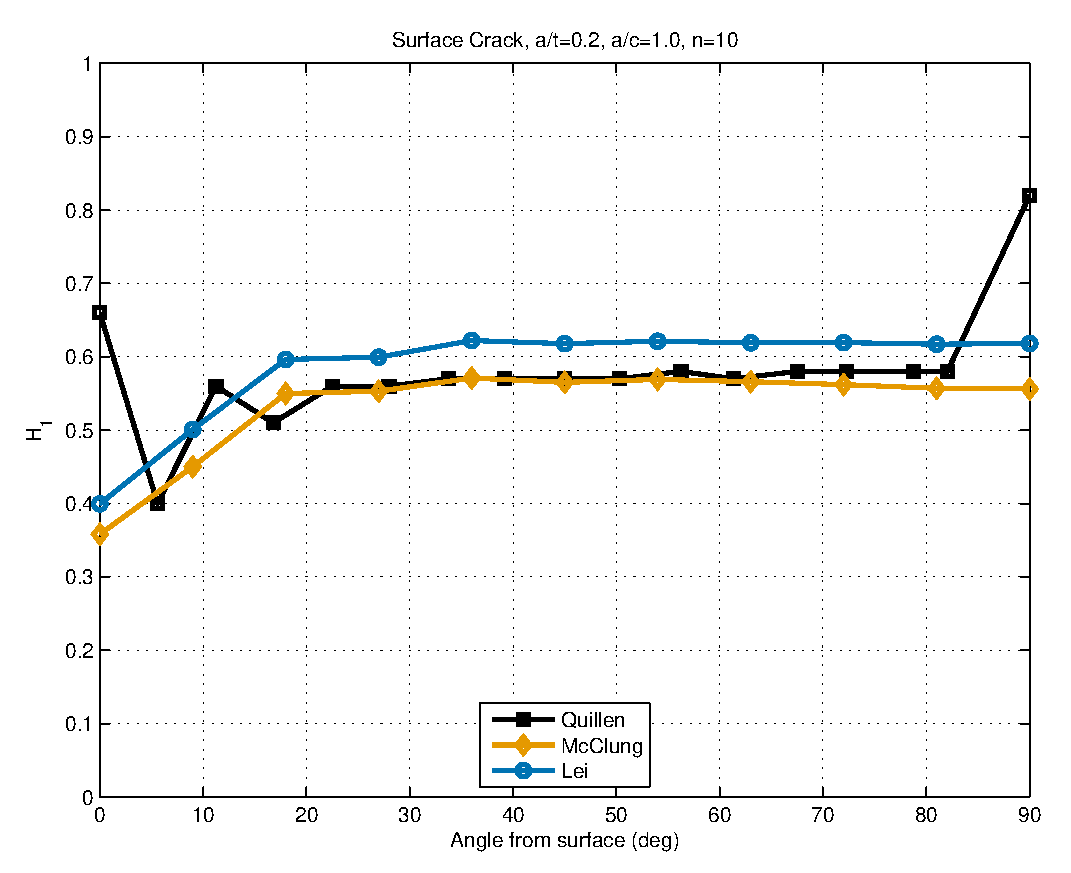
\includegraphics[width=0.6\columnwidth]{model3_n10}
  \caption[\hone comparison between \citeauthor{quillen2005}, McClung et al., and Lei, model 3, \(n=10\)]{\hone comparison between \citet{quillen2005}, McClung et al., and Lei, model 3, \(n=10\) \label{fig:model3_n10_2005}}
\end{figure}
\begin{figure}
  \centering
  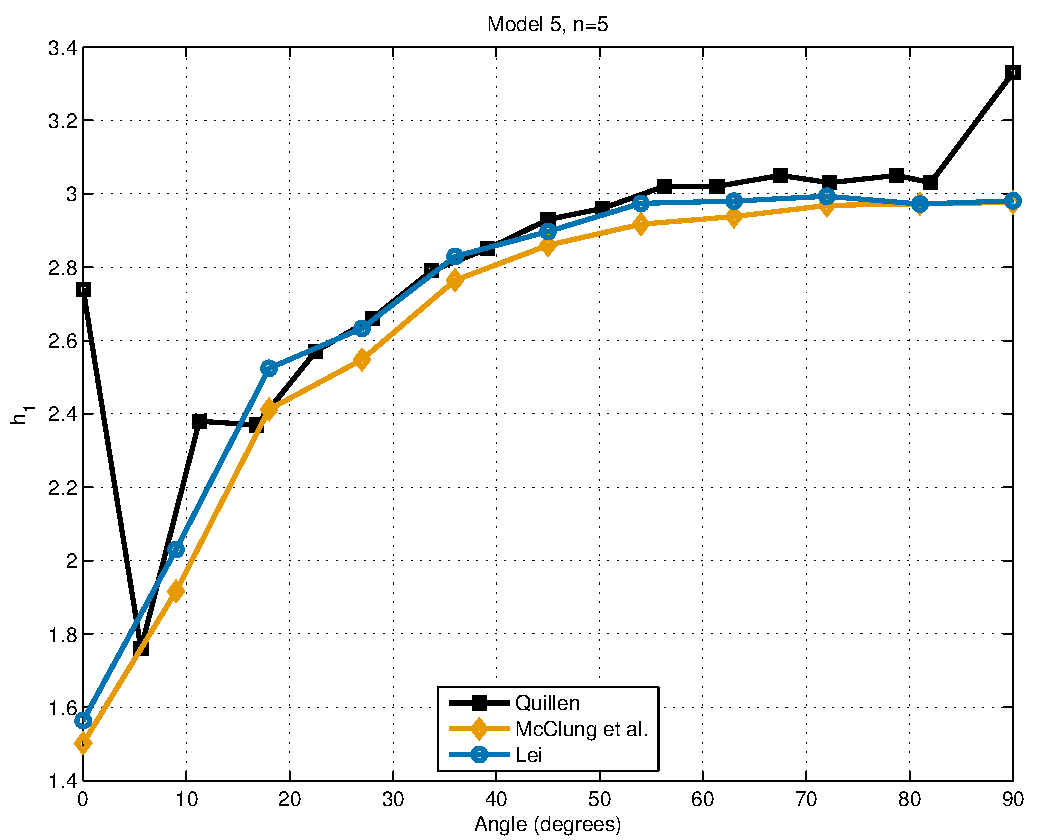
\includegraphics[width=0.6\columnwidth]{model5_n5}
  \caption[\hone comparison between \citeauthor{quillen2005}, McClung et al., and Lei, model 5, \(n=5\)]{\hone comparison between \citet{quillen2005}, McClung et al., and Lei, model 5, \(n=5\) \label{fig:model5_n5_2005}}
\end{figure}

\Cref{chap:app-quillen-rework} shows more detail on the development of some early Python programs used to create and analyze the plate and crack geometries shown in \Cref{fig:geometries}.
For each of the nine geometries, finite element models with varying numbers of elements were created.
For each finite element mesh, one linear elastic and three Ramberg-Osgood elastic-plastic models were analyzed, and \J values were stored in the Abaqus ODB.
Finally, \hone values were calculated from the \J values to test for convergence and verification against earlier models.
A total of 144 models were analyzed, including 36 elastic models (nine geometries by four mesh densities) and 108 elastic-plastic models (nine geometries by four mesh densities by three Ramberg-Osgood hardening exponents).
Solving all the models required approximately 43 hours on one quad-core AMD Opteron compute cluster node, and created \SI{103}{\giga\byte} of output data. Extracting \hone data from the ODB files took only 7 minutes.
Mesh convergence for one model is shown in \Cref{fig:mesh-convergence}, and convergence on the ratio of \Jpl:\Jel is shown in \Cref{fig:j-convergence}.
Note that the mesh convergence is not due simply to creating smaller elements along the crack front.
As shown in \Cref{fig:model1-3-meshes}, the number of elements along the crack front only increases from 21 to 25.
Adding additional elements outside the crack region has an effect on the \J and \hone values calculated, indicating that this model set needs further development.
However, all three anomalous \hone results in \citet{quillen2005} have been eliminated, as shown in \Cref{fig:model1}.
The root cause of the anomalies (errors in the original files generated by FEACrack, possible unrecorded modifications to the files, bugs corrected in Abaqus, etc.) is still unknown.

  \begin{figure}[tbp]
    \centering
    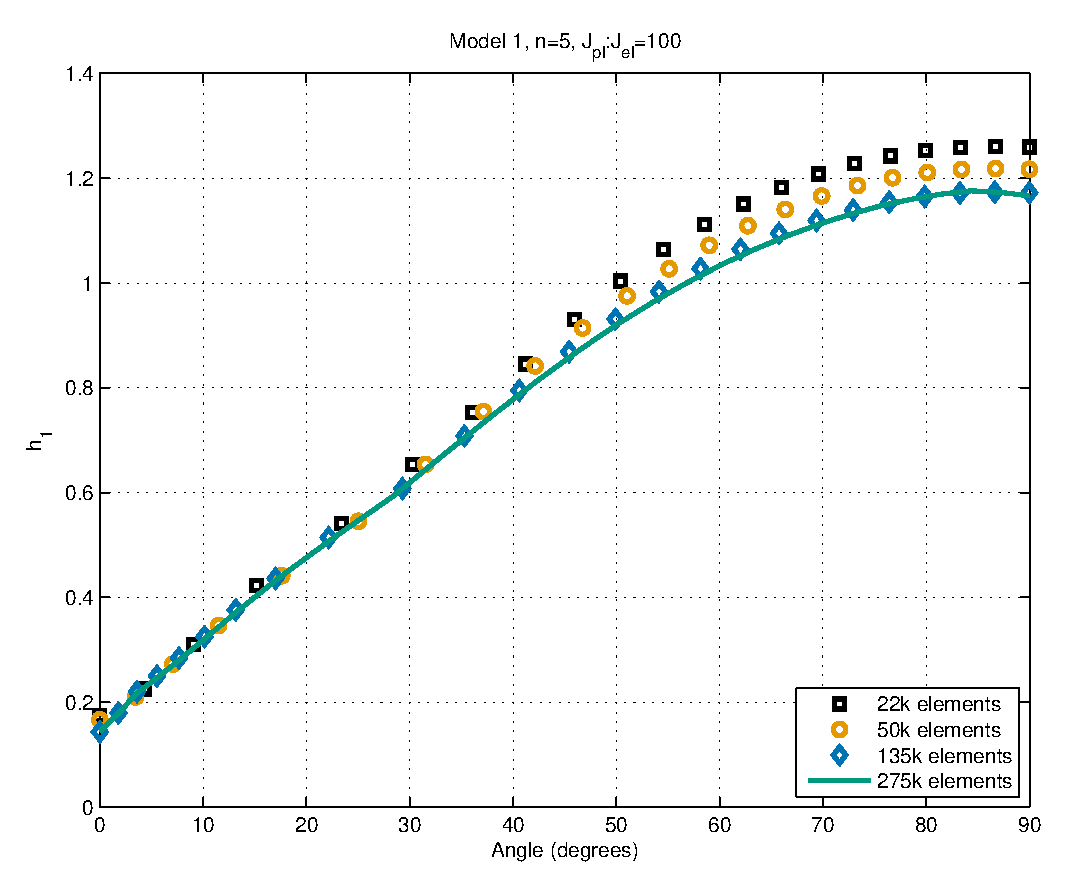
\includegraphics[width=0.6\columnwidth]{model1_n5_mesh_convergence}
    \caption{McClung et al. model 1 mesh convergence\label{fig:mesh-convergence}}
  \end{figure}
  \begin{figure}[tbp]
    \centering
    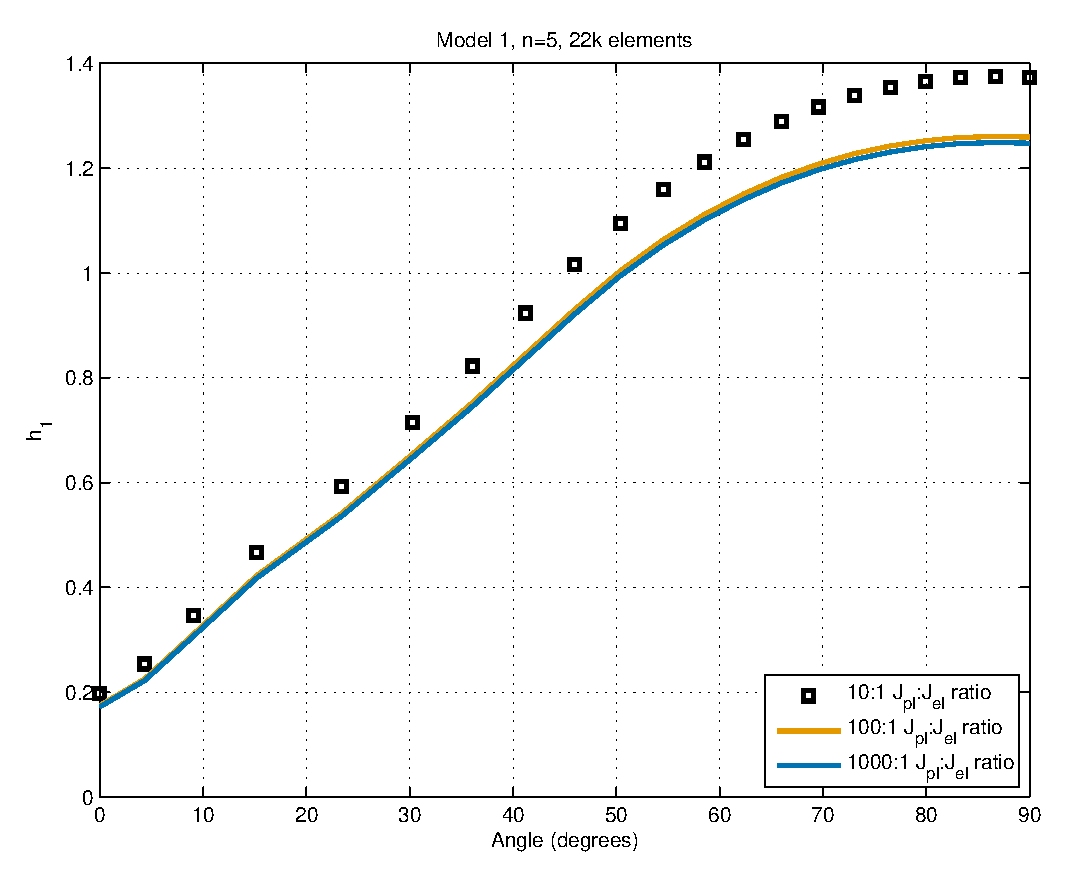
\includegraphics[width=0.6\columnwidth]{model1_n5_J_convergence}
    \caption{McClung et al. model 1 \J ratio convergence\label{fig:j-convergence}}
  \end{figure}

  \begin{figure}[tbp]
    \centering
    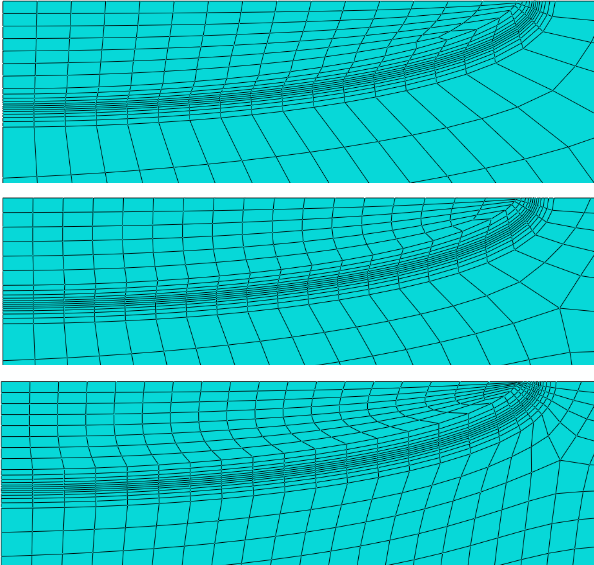
\includegraphics[width=0.6\columnwidth]{model1-3-meshes}
    \caption{McClung et al. model 1 crack front mesh detail\label{fig:model1-3-meshes}}
  \end{figure}
  \begin{figure}[tbp]
    \centering
    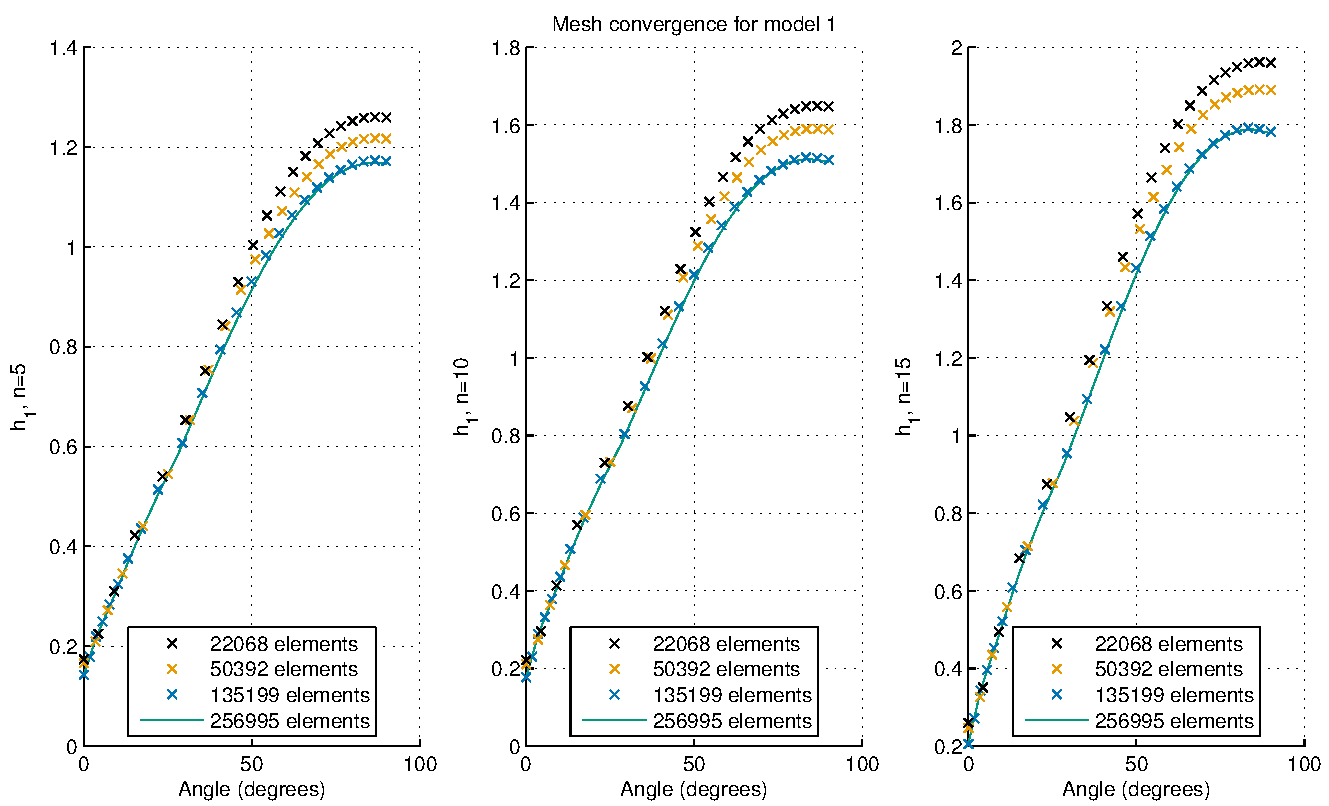
\includegraphics[width=\columnwidth]{h1_model1}
    \caption{\hone comparison between McClung et al., Lei, and Renfro, model 1 \label{fig:model1}}
  \end{figure}

\FloatBarrier
\section{Load Separation Verifications}
\label{sec:loadsepverification}

A brief check of the results of the \citet{sharobeamlandes1993} load separation results for surface cracks in tension was performed.
The six data points used in \Cref{fig:bet_Sij_original} were correlated back to specific crack sizes, and the most similar surface crack models from the TASC geometry set, \((\frac{a}{c}, \frac{a}{t}) = (0.6, 0.2), (0.6, 0.4), (0.6, 0.6), (1.0, 0.4)\), were adapted to include tension boundary conditions.
Remote tensile stress versus total CMOD and plastic CMOD for the four crack shapes is shown in \Cref{fig:stress-cmod-tension}.
The separation parameters \Sij using data from \((\frac{a}{c}, \frac{a}{t}) = (0.6, 0.6)\) as the reference curve is shown in \Cref{fig:sij_cmodpl}, and is limited to CMOD values greater than 0.01 in order to emphasize the regions with significant plastic behavior.
Finally, the correlation between \Sij and the effective uncracked ligament length for the original work from \citeauthor{sharobeamlandes1993} and for the current study are shown in \Cref{fig:sij_bet}, where both plots show relatively linear trends.
\begin{figure}[tbp]
\centering
\begin{minipage}{0.45\textwidth}
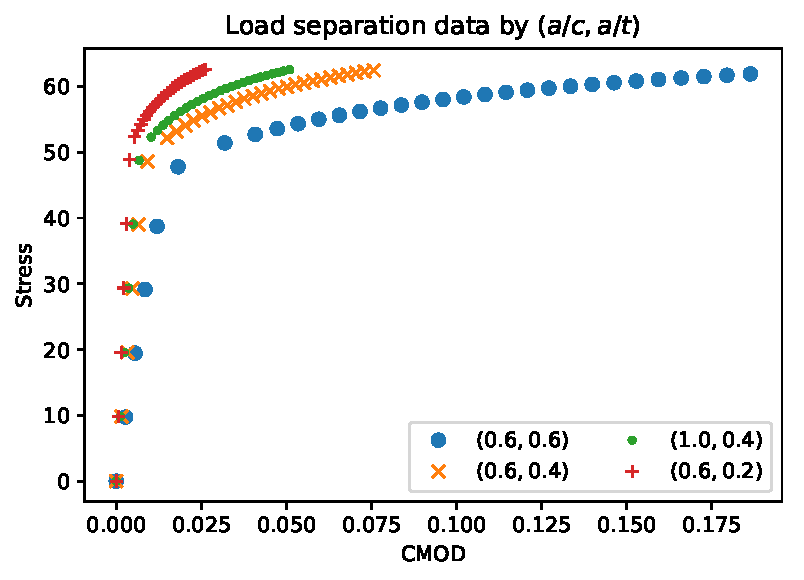
\includegraphics[width=\textwidth]{loadsep-stress-cmod-tension}
\subcaption{\label{fig:stress-cmod} Tensile stress versus CMOD}
\end{minipage}
\begin{minipage}{0.45\textwidth}
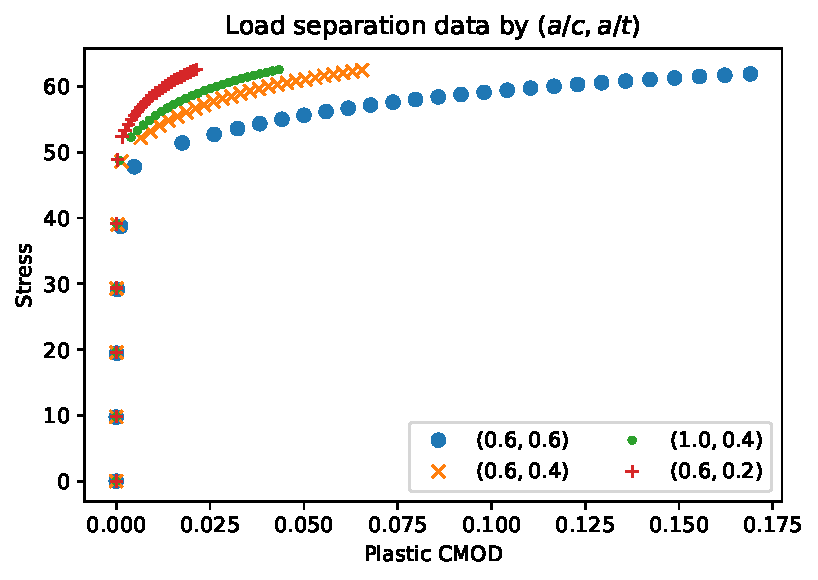
\includegraphics[width=\textwidth]{loadsep-stress-cmodpl-tension}
\subcaption{\label{fig:stress-cmodpl} Tensile stress versus plastic CMOD}
\end{minipage}
\caption{\label{fig:stress-cmod-tension} Initial load separation applied to surface cracks in tension}
\end{figure}
\begin{figure}[tbp]
\centering
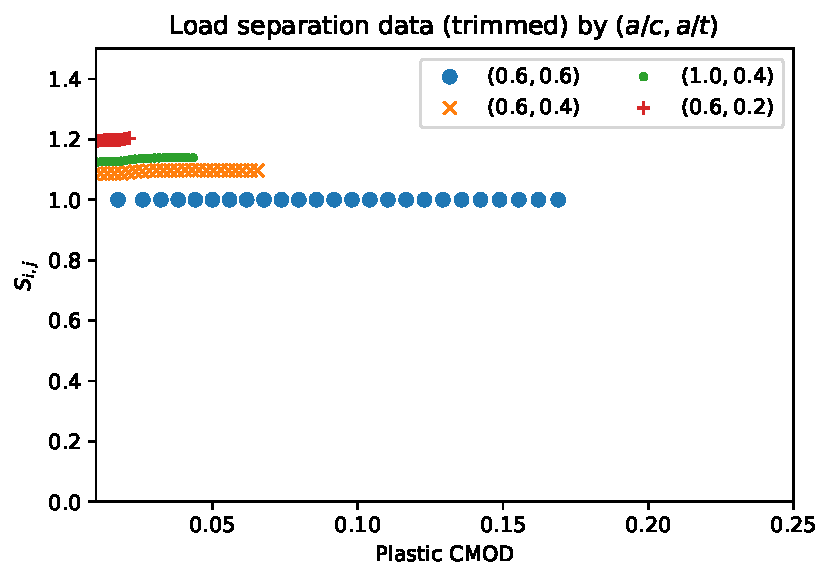
\includegraphics[width=0.8\textwidth]{cmodpl_Sij_tension}
\caption{\label{fig:sij_cmodpl} Separation parameter values versus plastic CMOD}
\end{figure}
\begin{figure}[tbp]
\centering
\begin{minipage}{0.45\textwidth}
\includegraphics[width=\textwidth]{load-sep-tension-sl-2}
\subcaption{\label{fig:load-sep-tension-sl} Annotated from \cite{sharobeamlandes1993}}
\end{minipage}
\begin{minipage}{0.45\textwidth}
\includegraphics[width=\textwidth]{bet_Sij_tension}
\subcaption{\label{fig:load-sep-tension-mwr} From current work}
\end{minipage}
\caption{\label{fig:sij_bet} Separation parameter values versus effective uncracked ligament length}
\end{figure}

\FloatBarrier

\section{Verification of Two TASC Cases}
\label{sec:verification-tasc}

The next chapter will show the development of a set of modeling tools to study surface cracks in flat plates, using FEACrack, Python, and WARP3D.
This section details the first use of these tools in verifying two tension models from \citeauthor{allenwells2014} (\citeyear{allenwells2014}), and then to solve an intermediate case, demonstrating the limits of the interpolation methodology.
Details of the algorithms used in the Python programs are given in \Crefrange{sec:preprocess}{sec:postprocess}.

\subsection{Identified Gaps in Interpolation Data}

\citeauthor{allenwells2014} built a set of 600 finite element models of surface cracks in tension, covering all combinations of
\begin{align*}
\frac{a}{t} &= 0.2, 0.4, 0.6, 0.8 & \frac{E}{\Sys} &= 100, 200, 300, 500, 700, 1000 \\
\frac{a}{c} &= 0.2, 0.4, 0.6, 0.8, 1.0 & n &= 3, 4, 6, 10, 20.
\end{align*}
Results for a set of models with \(\frac{a}{t}=0.6\) and \(n=6\) are shown in \Cref{fig:aspect-ratio-gap,fig:modulus-gap}.
The first figure shows a large gap between the results for cases \(\frac{a}{c}=0.2\) and \(\frac{a}{c}=0.4\), and the second figure shows a similar gap between the results for cases \(\frac{E}{\Sys}=100\) and \(\frac{E}{\Sys}=200\).
In each figure, normalized CMOD values for the more extreme case nearly double at comparable normalized stress levels, and the normalized \J values for the more extreme case are reduced by almost half at identical normalized CMOD levels.
As the authors use the solved models in a linear interpolation method, they identified a potential need for additional models with \(\frac{a}{c}=0.3\) and \(\frac{E}{\Sys}=150\), since there is no guarantee that the cracked plates exhibit linear behavior over such a wide range of results.
\begin{figure}[tbp]
\centering
\includegraphics[width=0.7\columnwidth]{aspect-ratio-gap}
\caption[Gap in results for very wide aspect ratios]{\label{fig:aspect-ratio-gap} Gap in results for very wide aspect ratios \citep{allenwells2014}}
\end{figure}
\begin{figure}[tbp]
\centering
\includegraphics[width=0.7\columnwidth]{modulus-gap}
\caption[Gap in results for very low elastic modulus values]{\label{fig:modulus-gap} Gap in results for very low elastic modulus values \citep{allenwells2014}}
\end{figure}

\Cref{chap:app-verification-allen-wells} details the use of FEACrack \citep{feacrack} and WARP3D \citep{warp3d} to replicate the published results for the cases
\begin{align*}
\frac{a}{t} &= 0.6 & \frac{E}{\Sys} &= 100 \text{ and } 200\\
\frac{a}{c} &= 0.6 & n &= 6
\end{align*}
and the remainder of this section will show the results of a purpose-built model for \(\frac{E}{\Sys} = 150\) compared to an interpolated model using results from \(\frac{E}{\Sys}=100\) and \(\frac{E}{\Sys}=200\).

\subsection{Applying Procedure to New Material Model (\(\frac{E}{\Sys} = 150\))}

After modifying the \(\frac{E}{\Sys} = 200\) model from \Cref{chap:app-verification-allen-wells} to use \(E = 150\) and leaving the normalized remote displacement at 0.0550, the new material model was solved.
As seen in \Cref{fig:e150_1}, the remote displacement was not high enough to place the model into the plastic regime, so the remote displacement was increased to 0.080.
The result of the new displacement is shown in \Cref{fig:e150_2}, and has clearly reached the plastic regime.
Later models used the secant method to adjust boundary conditions to meet a desired amount of plastic behavior, and reached a CMOD of roughly 0.03.
\begin{figure}[tbp]
\centering
\includegraphics[width=0.8\columnwidth]{e150_1}
\caption{\label{fig:e150_1} First attempt at new material model}
\end{figure}
\begin{figure}[tbp]
\centering
\includegraphics[width=0.8\columnwidth]{e150_2}
\caption{\label{fig:e150_2} Second attempt at new material model}
\end{figure}

Finally, by comparing the \(\frac{E}{\Sys} = 150\) FEA results to the interpolated TASC result from \Cref{fig:tasc_interp_outputs}, the FEA results are slightly more compliant in the elastic regime, and a sharper transition to the plastic regime at higher stress levels.
The two results differ by 5\% or less, as shown in \Cref{fig:e100_150_200_verification}.
\begin{figure}[tbp]
\centering
\includegraphics[width=0.8\columnwidth]{e100_150_200_verification}
\caption{\label{fig:e100_150_200_verification} Comparison of normalized FEA results, interpolated result, and TASC raw data}
\end{figure}

\subsection{Plotting CMOD, \J and \(\phi\)}

The final data to extract from the FEA results are values for the \J integral at each load increment. \J is a function of both load and position along the crack front, measured by the angle \(\phi\) from the free surface of the plate.
An example of the \J-\(\phi\)-CMOD relationship from \cite{allenwells2014} is shown in \Cref{fig:j-phi-cmod-paa}, while a comparable relationship from the current models is shown in \Cref{fig:j-phi-cmod-mwr}.
In both cases, higher CMOD values correlate with higher \J values, and \J values at a given CMOD are higher deep in the crack than at the free surface.
\begin{figure}[bp]
\centering
\includegraphics[width=0.8\columnwidth]{j-phi-cmod-paa}
\caption[Example relationship between \(\J(\phi)\) and CMOD from TASC]{\label{fig:j-phi-cmod-paa} Example relationship between \(\J(\phi)\) and CMOD from TASC\citep{allenwells2014}}
\end{figure}

\begin{figure}[tbp]
\centering
\includegraphics[width=0.8\columnwidth]{j-phi-cmod-mwr}
\caption{\label{fig:j-phi-cmod-mwr} Example relationship between \(\J(\phi)\) and CMOD}
\end{figure}


\chapter{Research Plan for Bending Models and Modified TASC Program}
\label{chap:research-plan}

Having validated an initial set of models against existing tensile results for \hone, load separation, and TASC in \Cref{chap:verification-tensile-sc}, the same modeling techniques can be applied to the ultimate goal of constructing a database of bending model results for the modified TASC program.
\J and CMOD results from WARP3D will be compared to results from Abaqus for identical geometry and material properties.
Additional EPRI \hone results will be generated for plates in bending, and the load separation technique will be applied to a set of bending results.
EPRI \hone and load separation methods offer an alternative to the TASC interpolation method.
All three types of analyses will use identical finite element meshes, removing one possible source of error when comparing results.
The work planned in each section of this chapter all fit into a encompassing research plan:
\begin{itemize}
\item a consistent set of models must be created for all three analysis types;
\item the 600 solutions required to build the bending database for TASC require automated adjustment of boundary conditions to ensure results are useful for \J-CMOD extrapolation; and
\item identical finite element meshes must be used for verification studies between Abaqus and WARP3D, for EPRI \hone calculations, and load separation calculations.
\end{itemize}

\section{Creating Plate Models}
\label{sec:preprocess}

All the surface crack models analyzed are similar in a parametric sense: each is a rectangular block of material with symmetric geometry and boundary conditions across the \(x\) and \(z\) axes.
Each surface crack has a semi-elliptical profile in the \(xy\) plane centered at the origin.
Since the bending models will be subjected to much larger displacements than tension models, the generic FEACrack model used for all geometries and materials is set to use a non-linear kinematic finite-strain element formulation supporting large rotations.
Each plate subjected to bending loads is in 4-point bending with loads and supports acting in the \(y\) direction, and each plate subjected to tensile loads is loaded in the \(z\) direction.
Additionally, each plate analyzed should minimize finite width effects and ensure the crack face is in a state of pure bending.
Thus, for a plate of thickness \(t\) and crack size defined by \(\frac{a}{c}\) and \(\frac{a}{t}\),
\begin{align*}
W &= 5 \max{(c, t)} \\
S_\text{inner} &= W \\
S_\text{outer} &= 2W \\
L &= \max{(1.1 (S_\text{outer}), 2W)}
\end{align*}
where \(S_\text{inner}\) and \(S_\text{outer}\)
are only defined for plates in bending and are shown in \Cref{fig:mesh-iso-dimensioned}.
\begin{figure}[tbp]
\centering
\includegraphics[width=\columnwidth]{mesh-iso-dimensioned}
\caption{\label{fig:mesh-iso-dimensioned}Model dimensions for plates in bending}
\end{figure}
Two example plates are shown in \Cref{fig:bend_ac02_at08_E0100_n03,fig:bend_ac10_at02_E0100_n03}, where each plate occupies extreme positions in terms of the crack geometry (and the plate width and length which are functions of crack width).
\begin{figure}[tbp]
\centering
\includegraphics[width=\textwidth]{bend_ac02_at08_E0100_n03}
\caption{\label{fig:bend_ac02_at08_E0100_n03} Plate model, \(\frac{a}{c}=0.2\), \(\frac{a}{t}=0.8\)}
\end{figure}
\begin{figure}[tbp]
\centering
\includegraphics[width=\textwidth]{bend_ac10_at02_E0100_n03}
\caption{\label{fig:bend_ac10_at02_E0100_n03} Plate model, \(\frac{a}{c}=1.0\), \(\frac{a}{t}=0.2\)}
\end{figure}

After the geometry and mesh for a given cracked plate have been defined, the elastic modulus \(E\) and the plastic stress-strain curve must be defined.
Finally, each combination of plate geometry, mesh, and material properties must be written into separate WARP3D input files for analysis.
An algorithm for constructing these input files is given in \Cref{alg:plate-creator}, a Python version of the algorithm for a subset of the problem space is given in \Cref{lst:plate-creator,lst:bend-config}, and an overall flow chart of the program is given in \Cref{fig:plate-creator-flowchart}.
The \verb|numpy| numeric Python libraries \cite{numpy} are used throughout the plate creation process to simplify any array-based operations. 
\begin{algorithm}[tbp]
  \caption{Plate Creator}
  \label{alg:plate-creator}
  \begin{algorithmic}
    \Procedure{Plate Creator}{} \Comment{Create a series of WARP3D input files}
    \State Read lists of $\frac{a}{t}$, $\frac{a}{c}$, $\frac{E}{\sigma_{\text{ys}}}$, $n$ values from configuration
    \State \Comment{typically: $0.2 \leq \frac{a}{t} \leq 0.8$, $0.2 \leq \frac{a}{c} \leq 1.0$, $100 \leq \frac{E}{\sigma_\text{ys}} \leq 1000$, $3 \leq n \leq 20$}
    \State Read $t$, $\sigma_\text{ys}$, global .elt file from configuration
    \State \Comment{typically: $t=1$, $\sigma_\text{ys}=1$, and global .elt file = 'bend.elt'}
    \ForAll{($\frac{a}{t}$ values, $\frac{a}{c}$ values)}
      \State $(a, c, L, W, S_{\text{in}}, S_{\text{out}}) \gets \Call{Set Geometry}{\text{global .elt file}, \frac{a}{c}, \frac{a}{t}, t}$
      \State $\text{generic mesh} \gets \Call{Build Mesh}{\text{global .elt file}, a, c, t, L, W, S_{\text{in}}, S_{\text{out}}}$
      \State \Comment{creates an input file with an arbitrary material for every combination of $\frac{a}{c}$ and $\frac{a}{t}$}
      \ForAll{($\frac{E}{\sigma_\text{ys}}$ values, $n$ values)}
        \State $E \gets (\frac{E}{\sigma_\text{ys}})(\sigma_\text{ys})$
        \State $\text{WARP3D input} \gets \Call{Set Material}{\text{generic mesh}, E, \sigma_\text{ys}, n}$
        \State \Comment{creates an input file for every combination of $\frac{a}{c}$, $\frac{a}{t}$, $E$, and $n$}
      \EndFor
    \EndFor
    \EndProcedure
  \end{algorithmic}
\end{algorithm}
\begin{Spacing}{1}
\begin{lstlisting}[language=Python,caption={Python implementation of Plate Creator algorithm}, label=lst:plate-creator]
# plate_creator.py
import preprocess as pre
from bend_config import aspect_ratio_list, depth_ratio_list
from bend_config import plate_thickness, E_Sys_ratio_list
from bend_config import Sys, n_list
from bend_config import elt_global_template_filename

for depth_ratio in depth_ratio_list:
    for aspect_ratio in aspect_ratio_list:
        (a, c, W, t, L,
         S_inner, S_outer) = pre.calculate_geometry(
                     elt_global_template_filename,
                     depth_ratio, aspect_ratio,
                     plate_thickness)
        geom_filename = pre.build_mesh(
                elt_global_template_filename, a, c, L, W, t,
                S_inner, S_outer)
        print("Wrote generic mesh {0}".format(geom_filename))
        for n in n_list:
            for E_Sys_ratio in E_Sys_ratio_list:
                E = Sys*E_Sys_ratio
                model_filename = pre.change_material_properties(
                        inp_filename=geom_filename,
                        E=E, Sys=Sys, n=n)
                print("Wrote {0}".format(model_filename))
\end{lstlisting}
\end{Spacing}
\begin{Spacing}{1}
\begin{lstlisting}[language=Python,caption={Python implementation for subset of geometry and material configurations}, label=lst:bend-config]
# bend_config.py
aspect_ratio_list = [0.2, 0.4, ]
depth_ratio_list = [0.2, 0.4, 0.6, 0.8, ]
plate_thickness = 1.0
E_Sys_ratio_list = [100.0, 200.0, 300.0, 500.0, 700.0, 1000.0, ]
Sys = 1.0
n_list = [3, 4, 6, 10, 20, ]
elt_global_template_filename = 'bend.elt'
\end{lstlisting}
\end{Spacing}
\begin{figure}
\centering
\includegraphics[width=0.5\columnwidth]{plate_creator_flowchart}
\caption{\label{fig:plate-creator-flowchart} Overall flowchart of bending model creation program}
\end{figure}


The remaining algorithms will be shown only as pseudocode in order to emphasize the structure of the algorithms instead of their specific implementation.
Readers interested in the Python implementation can download a copy of the Python source files from \url{https://github.com/mikerenfro/phd}.

\subsection{Defining Plate Model Geometry}

\Cref{alg:set_geometry} uses \Cref{alg:get_type} to determine if the model is in bending or tension, and calculates the necessary plate dimensions from given values for crack aspect ratio, crack depth ratio, and plate thickness.
\Cref{alg:get_type} looks through an FEACrack input file for specific commands in the file's notes field and commands.
If a traction in the \(y\) direction is defined in the notes field, and two rigid roller surfaces are found in the model commands, the model is assumed to represent a plate in bending.
Otherwise, the model is assumed to represent a plate in tension.
\Cref{alg:build_mesh} has four main tasks: to first use \Cref{alg:get_elt_filename} to define the name of a new FEACrack input file, to copy the generic FEACrack input file to the new name, to use \Cref{alg:adjust_roller_positions} to modify the roller locations for bending models, and finally running FEACrack with command arguments to create a WARP3D input file with the correct plate geometry and crack size.
\Cref{alg:get_elt_filename} takes the name of the generic FEACrack input file and a list of dimension values, and defines a new FEACrack input filename with the dimension values included.
\Cref{alg:adjust_roller_positions} searches an FEACrack input file for commands representing the position of rollers, and changes their \(z\) dimensions to match \Sinner and \Souter.
\begin{algorithm}[tbp]
  \caption{Set Geometry}
  \label{alg:set_geometry}
  \begin{algorithmic}
    \Procedure{Set Geometry}{$\text{global .elt file}, \frac{a}{c}, \frac{a}{t}, t$} \Comment{Calculate plate dimensions}
    \State $a \gets (\frac{a}{t})t$
    \State $c \gets a (\frac{a}{c})^{-1}$
    \If{$c > t$}
      \State $W \gets 5c$
    \Else
      \State $W \gets 5t$
    \EndIf
    \State $\text{model type} \gets \Call{Get Type}{\text{global .elt file}}$
    \If{model type = 'bending'}
      \State $\Sinner \gets W$
      \State $\Souter \gets 2W$
      \If{$2 W > 1.1 \Souter$}
        \State $L \gets 2 W$
      \Else
        \State $L \gets 1.1 \Souter$
      \EndIf
    \Else
      \State $\Sinner \gets \text{Null}$
      \State $\Souter \gets \text{Null}$
      \State $L \gets 2 W$
    \EndIf
    \State \textbf{return} $(a, c, W, L, \Sinner, \Souter)$
    \EndProcedure
  \end{algorithmic}
\end{algorithm}

\begin{algorithm}[tbp]
  \caption{Get Type}
  \label{alg:get_type}
  \begin{algorithmic}
    \Procedure{Get Type}{global .elt file}
      \State \Comment{determine if a .elt file is for a bending or a tension model}
      \If{'"*use bottom load pin plate ty ' found in 'Notes:' field}
        \If{'RigidSurfaceData\_Radius' found twice}
          \If{'RigidSurfaceData\_PinLocation' found twice}
            \State model type $\gets$ 'bending'
          \Else
            \State model type $\gets$ 'invalid'
          \EndIf
        \EndIf
      \Else
        \State model type $\gets$ 'tension'
      \EndIf
      \State \textbf{return} model type
    \EndProcedure
  \end{algorithmic}
\end{algorithm}

\begin{algorithm}[tbp]
  \caption{Build Mesh}
  \label{alg:build_mesh}
  \begin{algorithmic}
    \Procedure{Build Mesh}{{global .elt file}, $a$, $c$, $t$, $L$, $W$, $\Sinner$, $\Souter$}
      \State \Comment{use FEACrack create a WARP3D input file with an arbitrary material}
      \State {model .elt file} $\gets$ \Call{Get Elt Filename}{{global .elt file}, $a$, $c$, $L$, $W$, $t$} 
      \State \Comment{'bend\_ac$(\frac{a}{c})$\_at$(\frac{a}{t})$\_L$(L)$\_W$(W)$.elt'}
      \State Copy {global .elt file} to {model .elt file}
      \If{$\Sinner \neq \text{Null} \AND \Souter \neq \text{Null}$}
        \State \Call{Adjust Roller Positions}{model .elt file, $\Sinner$, $\Souter$}
      \EndIf
      \State Run FEACrack program on model .elt file, using $a$, $2c$, $t$, $L$, and $W$
      \State \textbf{return} \text{generic mesh file} \Comment{'bend\_ac$(\frac{a}{c})$\_at$(\frac{a}{t})$\_L$(L)$\_W$(W)$\_wrp.inp'}
    \EndProcedure
  \end{algorithmic}
\end{algorithm}

\begin{algorithm}[tbp]
  \caption{Get Elt Filename}
  \label{alg:get_elt_filename}
  \begin{algorithmic}
    \Procedure{Get Elt Filename}{global .elt file, $a$, $c$, $L$, $W$, $t$}
      \State \Comment{determine the name of a .elt file for a given geometry}
      \State prefix $\gets$ global .elt file basename \Comment{'bend'}
      \State middle $\gets$ '\_ac$(\frac{a}{c})$\_at$(\frac{a}{t})$\_L$(L)$\_W$(W)$'
      \State suffix $\gets$ '.elt'
      \State \textbf{return} prefix + middle + suffix \Comment{'bend\_ac$(\frac{a}{c})$\_at$(\frac{a}{t})$\_L$(L)$\_W$(W)$.elt'}
    \EndProcedure
  \end{algorithmic}
\end{algorithm}

\begin{algorithm}[tbp]
  \caption{Adjust Roller Positions}
  \label{alg:adjust_roller_positions}
  \begin{algorithmic}
    \Procedure{Adjust Roller Positions}{model .elt file, $\Sinner$, $\Souter$}
    \State \Comment{move roller positions in .elt file to $\Sinner$ and $\Souter$}
    \If{first 'RigidSurfaceData\_PinLocation' found in model .elt file}
      \State Change $z$ value of location to $\Sinner$
    \EndIf
    \If{second 'RigidSurfaceData\_PinLocation' found in model .elt file}
      \State Change $z$ value of location to $\Souter$
    \EndIf
    \EndProcedure
  \end{algorithmic}
\end{algorithm}

\subsection{Defining Material Properties}

\Cref{alg:set_material} calls \Cref{alg:get_specific_model_filename} to determine the name of a WARP3D input file for a specific material, copies the WARP3D input file for the current geometry to the new name, and examines the new WARP3D input file for lines representing the plastic behavior of the material. Those lines are replaced with the results of \Cref{alg:lppl} for a given elastic modulus, yield strength, and hardening exponent.
\Cref{alg:get_specific_model_filename} takes the name of the WARP3D file for the current geometry and defines a new WARP3D input filename with the elastic modulus and hardening exponent values included.
\Cref{alg:lppl} defines a set of plastic strain values that are finely spaced near the onset of yield, and increasingly coarse as plastic strain increases, and uses a power law relationship to define the corresponding set of true stress values. This ensures a smooth transition from linear behavior without using an excessive total number of points on the curve.

\begin{algorithm}[tbp]
  \caption{Set Material}
  \label{alg:set_material}
  \begin{algorithmic}
    \Procedure{Set Material}{generic .inp file, $E$, $\sigma_\text{ys}$, $n$}
    \State \Comment{modify arbitrary material parameters in input file to specified values}
    \State specific .inp file $\gets$ \Call{Get Specific Model Filename}{generic .inp file, $E$, $\sigma_\text{ys}$, $n$}
    \State \Comment{'bend\_ac$(\frac{a}{c})$\_at$(\frac{a}{t})$\_L$(L)$\_W$(W)$\_E$(E)$\_n$(n)$\_wrp.inp'}
    \State Copy generic .inp file to specific .inp file
    \If{'stress-strain curve      1' found in specific .inp file}
      \State change stress-strain curve data to \Call{LPPL}{$E$, $\sigma_\text{ys}$, $n$}
    \EndIf
    \State change $E$ value in specific .inp file
    \State \textbf{return} specific .inp file \Comment{'bend\_ac$(\frac{a}{c})$\_at$(\frac{a}{t})$\_L$(L)$\_W$(W)$\_E$(E)$\_n$(n)$\_wrp.inp'}

    \EndProcedure
  \end{algorithmic}
\end{algorithm}

\begin{algorithm}[tbp]
  \caption{Get Specific Model Filename}
  \label{alg:get_specific_model_filename}
  \begin{algorithmic}
    \Procedure{Get Specific Model Filename}{.inp filename, $E$, $\sigma_\text{ys}$, $n$}
      \State \Comment{determine the name of a specific .inp file for a given geometry and material parameters}
      \State prefix $\gets$ .inp file basename \Comment{'bend\_ac$(\frac{a}{c})$\_at$(\frac{a}{t})$\_L$(L)$\_W$(W)$\_wrp'}
      \State prefix $\gets$ prefix without last 4 characters
      \State \Comment{'bend\_ac$(\frac{a}{c})$\_at$(\frac{a}{t})$\_L$(L)$\_W$(W)$'}
      \State middle $\gets$ '\_E$(E)$\_n$(n)$'
      \State suffix $\gets$ '\_wrp.inp'
      \State \textbf{return} prefix + middle + suffix
      \State \Comment{'bend\_ac$(\frac{a}{c})$\_at$(\frac{a}{t})$\_L$(L)$\_W$(W)$\_E$(E)$\_n$(n)$\_wrp.inp'}
    \EndProcedure
  \end{algorithmic}
\end{algorithm}

\begin{algorithm}[tbp]
  \caption{LPPL}
  \label{alg:lppl}
  \begin{algorithmic}
    \Procedure{LPPL}{$E$, $\sigma_\text{ys}$, $n$} \Comment{calculate the plastic stress-strain curve for a power law material}
    \State $\epsilon_{\text{pl1}} \gets (0.001, 0.002, \cdots , 0.008)$
    \State $\epsilon_{\text{pl2}} \gets (0.013, 0.018, 0.023, 0.028)$
    \State $\epsilon_{\text{pl3}} \gets (0.038, 0.048, \cdots , 0.108)$
    \State $\epsilon_{\text{ys}} \gets \frac{\sigma_\text{ys}}{E}$
    \State $\epsilon \gets \epsilon_{\text{ys}} + (\epsilon_{\text{pl1}}, \epsilon_{\text{pl2}}, \epsilon_{\text{pl3}})$
    \State $\sigma \gets \sigma_\text{ys}  (\frac{\epsilon}{\epsilon_{\text{ys}}})^{\frac{1}{n}}$
    \State \textbf{return} $\epsilon$, $\sigma$
    \EndProcedure
  \end{algorithmic}
\end{algorithm}

\section{Solving Plate Models, Optimizing Boundary Conditions}
\label{sec:solve}

Now that the plate geometry, material properties, and boundary conditions are defined for a set of models, a procedure for solving for reaction forces, \J values, and CMOD values must be developed.
The boundary conditions applied to the model must be large enough to induce substantial amounts of plastic deformation, but not so large as to cause the model to exceed its material limits or become numerically unstable.
In \cite{allenwells2014}, the models were reported to have been deformed enough to cause the deformation level\nomenclature[1M]{\(M\)}{dimensionless deformation parameter for plates in bending}
\begin{align}
M &= \frac{r_{\phi} \Sys}{\J}
\end{align}
to drop below 20 or 25, but upon examining the TASC database, approximately half the models had minimum \(M\) values over 25, and about 10\% of the models had \(M\) values over 50, as seen in \Cref{fig:min-M-hist}.
Regardless of the exact deformation required, all models in the TASC database must contain enough data to perform accurate linear extrapolations from the \(\sigma\)-CMOD and \J-CMOD curves, similar to the curves shown in \Cref{fig:J-CMOD-extrapolation}.

\begin{figure}[tbp]
\centering
\includegraphics[width=0.7\columnwidth]{min_M_hist}
\caption{\label{fig:min-M-hist} Histogram of \(M\) results from TASC tension model database}
\end{figure}

\begin{figure}[tbp]
\centering
\includegraphics[width=0.7\columnwidth]{J-CMOD-extrapolation}
\caption[\J-CMOD graph used for extrapolation]{\label{fig:J-CMOD-extrapolation} \J-CMOD graph used for extrapolation \cite{allenwells2014}}
\end{figure}

\J{}-CMOD curves like the ones in \Cref{fig:J-CMOD-extrapolation,fig:J-phi-ac_02_at_02_E0100_n03,fig:J-phi-ac_10_at_08_E0500_n06} all show \J values that increase slowly in the linear elastic regime compared to the highly-plastic regime, but have widely varying \J and CMOD ranges.
Some cracks in bending will show lower \J values at the free surface than deep inside the crack, as shown in \Cref{fig:J-phi-ac_02_at_02_E0100_n03}, while others will show higher \J values at the free surface than deep inside the crack, as shown in \Cref{fig:J-phi-ac_10_at_08_E0500_n06}.
\begin{figure}[tbp]
\centering
\includegraphics[width=0.8\textwidth]{J_CMOD_bend_ac02_at02_L1100_W0500_E0100_n03_wrp}
\caption{\J-CMOD relationship at \(\phi=\) \SIlist{0;30;90}{\SIUnitSymbolDegree}: \(\frac{a}{c}=0.2\), \(\frac{a}{t}=0.2\), \(E=100\), \(n=3\) \label{fig:J-phi-ac_02_at_02_E0100_n03}}
\end{figure}
\begin{figure}[tbp]
\centering
\includegraphics[width=0.8\textwidth]{J_CMOD_bend_ac10_at08_L1100_W0500_E0500_n06_wrp}
\caption{\J-CMOD relationship at \(\phi=\) \SIlist{0;30;90}{\SIUnitSymbolDegree}: \(\frac{a}{c}=1.0\), \(\frac{a}{t}=0.6\), \(E=500\), \(n=6\) \label{fig:J-phi-ac_10_at_08_E0500_n06}}
\end{figure}
Since the goal with a bending model is to use enough deformation to make accurate linear extrapolations from the results, the criteria analogous to the \(M\) criteria from \cite{allenwells2014} is defined as
\begin{enumerate} \label{list:criteria}
\item the slope of a linear fit to the last 20\% of the \J-CMOD curve should be at least 20 times larger than the slope of the initial linear region of the \J-CMOD curve, and
\item the slope of the last 20\% of the \J-CMOD curve should be within 10\% of the slope of the previous 20\% of the \J-CMOD curve.
\end{enumerate}
The first criteria ensures that the model has deformed well beyond the linear elastic regime, and the second ensures that linear extrapolations will be relatively insensitive to additional deformation.
Using ratios of \J and CMOD values in both criteria removes variability due to material properties and crack geometry.
As \J at a given CMOD is a function of angle \(\phi\) from the free surface, the \J values for \(\phi=30{\SIUnitSymbolDegree}\) are used to avoid effects of both the stress-free surface at \SI{0}{\SIUnitSymbolDegree} and constraint effects at \SI{90}{\SIUnitSymbolDegree}.

An algorithm for solving a set of models created by \Cref{alg:plate-creator} is shown in \Cref{alg:plate-runner}, with an overall flow chart shown in \Cref{fig:plate_runner_flowchart}.
For each combination of \(\frac{a}{c}\), \(\frac{a}{t}\), \(\frac{E}{\sigma_{\text{ys}}}\), and \(n\), it uses \Cref{alg:set_geometry} to calculate the cracked geometry.
It uses \Cref{alg:get_elt_filename,alg:get_generic_model_filename,alg:get_specific_model_filename} to identify relevant input files, and uses \Cref{alg:optimize_bc} to automate the process of modifying boundary conditions and solving the finite element models until the plates have been sufficiently deformed to satisfy the the list of criteria on \cpageref{list:criteria}.
The Python implementation of these algorithms makes use of the \verb|numpy| \cite{numpy}, \verb|scipy| \cite{scipy}, and  \verb|pandas| \cite{mckinney-proc-scipy-2010} libraries.
\verb|numpy| is used as a general-purpose numerical library for Python, \verb|scipy| is used for both linear regressions and optimizations, while \verb|pandas| is used for reading and filtering structured output files.
\begin{figure}
\centering
\includegraphics[width=0.75\columnwidth]{plate_runner_flowchart}
\caption{\label{fig:plate_runner_flowchart} Overall flowchart of bending model solution program}
\end{figure}


Looking more closely at the process for finding boundary conditions as shown in \Cref{alg:optimize_bc}, the following details must be considered.
All the materials examined have highly non-linear stress-strain (and load-displacement) behavior, where small changes in applied stresses or loads may cause large changes in strains or displacements.
Similarly, large changes in strain or displacement may only cause small changes in stress or reaction loads.
Displacement boundary conditions were used in \cite{allenwells2014}, which mimics common closed-loop control methods used in mechanical properties testing.
These boundary conditions were constant values applied on the face parallel to the crack front.
However, reaching a sufficient level of plastic deformation around the crack front may require much more displacement than required to reach yield, as shown in \Cref{fig:secant-1}.
\begin{figure}[tbp]
\centering
\includegraphics[width=0.8\columnwidth]{secant-1}
\caption{\label{fig:secant-1}Example stress-strain curve using linear plus power law (LPPL) formulation}
\end{figure}
Applying an incremental search to discover how much displacement is required to reach that level of plastic deformation would prove to be slow to converge (where small displacement steps cause even smaller changes in stress state for most of the search space) or inaccurate (where large displacement steps risk running outside the material's defined stress-strain data).
Considering a transformed stress-strain curve as shown in \Cref{fig:secant-2} where the starting point on the stress-strain curve is shown by the green square, the secant method should converge quickly to the target point shown by the orange circle.
\begin{figure}[tbp]
\centering
\includegraphics[width=0.8\columnwidth]{secant-2}
\caption{\label{fig:secant-2}LPPL stress-strain curve, transformed to find required strain level}
\end{figure}

The bending models require additional considerations to match experimental conditions, especially for larger plates.
A typical four-point bend test applies external forces with a set of inner cylindrical rollers, and the plate is supported by an outer set of cylindrical rollers, as shown in \Cref{fig:astm-e2899-4point-bend}.
Modeling the internal rollers as constant transverse displacement conditions along a plane parallel to the crack face will grow increasingly inaccurate as that plane rotates relative to the crack face.
Applying transverse tractions on all element faces coincident with the location of the inner roller solves this issue.
Because traction has units of force per unit area, the same traction value can be applied to each element, regardless of the element size.
\begin{figure}[tbp]
\centering
\includegraphics[width=0.8\columnwidth]{astm-e2899-4point-bend}
\caption[Four-point bend test configuration]{\label{fig:astm-e2899-4point-bend} Four-point bend test configuration \cite{astme2899}}
\end{figure}

However, moving from a strain- or displacement-controlled method to a stress- or force-controlled method complicates the root-finding methods used in the tension cases.
As the independent variable is now stress, and the dependent variable is now strain, this transforms the stress-strain curve to the form shown in \Cref{fig:secant-3,fig:secant-4}.
\begin{figure}[tbp]
\centering
\includegraphics[width=0.8\columnwidth]{secant-3}
\caption{\label{fig:secant-3}Example stress-strain curve using linear plus power law (LPPL) formulation, transformed to stress-controlled}
\end{figure}
\begin{figure}[tbp]
\centering
\includegraphics[width=0.8\columnwidth]{secant-4}
\caption{\label{fig:secant-4}Example stress-strain curve using linear plus power law (LPPL) formulation, transformed to find required stress level}
\end{figure}
The curve is now much less suitable for solution using the secant method: the neighborhood of starting point has a very shallow slope that will cause the next stress value to be much higher, either causing slow convergence in the case of an LPPL function with a semi-infinite domain, or simply exceeding the range of the stress-strain curve in the case of a finite set of stress-strain points.
However, using a simple incremental search method with step sizes equal to 10\% of the initial stress only takes a few steps to reach the neighborhood of the target stress value.
Other root-finding methods could be used to find the required stress value, such as bisection, false position, or Brent's method \cite{numericalrecipes1986}.
However, each of these methods requires the determination of a finite interval \([\sigma_a, \sigma_b]\) that surround the required stress value.
Though it is possible to set that interval to the domain of a finite set of stress-strain data points, this is impossible for an LPPL function with a semi-infinite domain.
Additionally, the open-ended nature of the slope ratio criteria on \cpageref{list:criteria} means that all stress values exceeding a minimum target value will meet that criteria.
Finally, having a finite number of load steps in the finite element model and the need to accurately model the transition to elastic-plastic behavior means that lower stress values meeting the criteria on \cpageref{list:criteria} are preferred.
All three of these factors lead to a conclusion that any root-finding method that requires no bracketing and whose proposed root values monotonically increase will find appropriate stress values that will allow accurate extrapolation without sacrificing detail in the transition to elastic-plastic behavior.
\begin{algorithm}[tbp]
  \caption{Plate Runner}
  \label{alg:plate-runner}
  \begin{algorithmic}
    \Procedure{Plate Runner}{} \Comment{Solve a series of WARP3D input files}
    \State Read lists of $\frac{a}{t}$, $\frac{a}{c}$, $\frac{E}{\sigma_{\text{ys}}}$, $n$ values from configuration
    \State \Comment{typically: $0.2 \leq \frac{a}{t} \leq 0.8$, $0.2 \leq \frac{a}{c} \leq 1.0$, $100 \leq \frac{E}{\sigma_\text{ys}} \leq 1000$, $3 \leq n \leq 20$}
    \State Read $t$, $\sigma_\text{ys}$, global .elt file from configuration
    \State \Comment{typically: $t=1$, $\sigma_\text{ys}=1$, and global .elt file = 'bend.elt'}
    \ForAll{($\frac{a}{t}$ values, $\frac{a}{c}$ values)}
      \State $(a, c, L, W, S_{\text{in}}, S_{\text{out}}) \gets \Call{Set Geometry}{\text{global .elt file}, \frac{a}{c}, \frac{a}{t}, t}$
      \ForAll{($\frac{E}{\sigma_\text{ys}}$ values, $n$ values)}
        \State $E \gets (\frac{E}{\sigma_\text{ys}})(\sigma_\text{ys})$
        \State {model .elt file} $\gets$ \Call{Get Elt Filename}{{global .elt file}, $a$, $c$, $L$, $W$, $t$} 
        \State \Comment{'bend\_ac$(\frac{a}{c})$\_at$(\frac{a}{t})$\_L$(L)$\_W$(W)$.elt'}
        \State {generic .inp file} $\gets$ \Call{Get Generic Model Filename}{{model .elt file}}
        \State \Comment{'bend\_ac$(\frac{a}{c})$\_at$(\frac{a}{t})$\_L$(L)$\_W$(W)$\_wrp.inp'}
        \State {specific .inp file} $\gets$ \Call{Get Specific Model Filename}{{generic .inp file}, $E$, $\sigma_\text{ys}$, $n$}
        \State \Comment{'bend\_ac$(\frac{a}{c})$\_at$(\frac{a}{t})$\_L$(L)$\_W$(W)$\_E$(E)$\_n$(n)$\_wrp.inp'}
        \If{\Call{Get Model Type}{specific .inp file} = 'bending'}
          \State ($z_{\text{in}}$, $z_{\text{out}}$) = \Call{Find Pin Locations}{specific .inp file}
        \EndIf
        \State \Call{Optimize BC}{specific .inp file, $a$, $c$, $L$, $W$, $t$, $z_{\text{in}}$, $z_{\text{out}}$, $E$, $n$}
        \State \Call{Postprocess}{specific .inp file}
      \EndFor
    \EndFor
    \EndProcedure
  \end{algorithmic}
\end{algorithm}

\begin{algorithm}[tbp]
  \caption{Get Generic Model Filename}
  \label{alg:get_generic_model_filename}
  \begin{algorithmic}
    \Procedure{Get Generic Model Filename}{model .elt file}
    \State prefix $\gets$ model .elt file basename \Comment{'bend\_ac$(\frac{a}{c})$\_at$(\frac{a}{t})$\_L$(L)$\_W$(W)$'}
    \State \textbf{return} prefix + '\_wrp.inp' \Comment{'bend\_ac$(\frac{a}{c})$\_at$(\frac{a}{t})$\_L$(L)$\_W$(W)$\_wrp.inp'}
\EndProcedure
  \end{algorithmic}
\end{algorithm}

\begin{algorithm}[tbp]
  \caption{Optimize BC}
  \label{alg:optimize_bc}
  \begin{algorithmic}
    \Procedure{Optimize BC}{.inp file, $a$, $c$, $L$, $W$, $t$, $z_{\text{in}}$, $z_{\text{out}}$, $E$, $\sigma_{\text{ys}}$, $n$}
    \State \Comment{Change Boundary Conditions for Model until Sufficient Deformation Applied}
    \State model type $\gets$ \Call{Get Model Type}{.inp file}
    \State initial BC $\gets$ \Call{Get Initial BC}{.inp file, $a$, $c$, $L$, $W$, $t$, $z_{\text{in}}$, $z_{\text{out}}$, $E$, $\sigma_{\text{ys}}$, $n$, model type}
    \If{model type = 'tension'}
      \State optimal BC $\gets$ \Call{Secant Method}{\Call{Run Model}{initial BC}}
      \State \Comment{with fixed values for .inp file, $a$, $c$, $L$, $W$, $t$, $z_{\text{in}}$, $z_{\text{out}}$, $E$, $n$, model type}
    \Else
      \State BC $\gets$ initial BC
      \While{$\Call{Run Model}{\text{initial BC}}>0$}
        \State \Comment{with fixed values for .inp file, $a$, $c$, $L$, $W$, $t$, $z_{\text{in}}$, $z_{\text{out}}$, $E$, $n$, model type}
        \State BC $\gets$ BC + 0.1 (initial BC)
      \EndWhile
      \State optimal BC $\gets$ BC
    \EndIf
    \State \textbf{return} optimal BC
    \EndProcedure
  \end{algorithmic}
\end{algorithm}

\Cref{alg:optimize_bc} uses \Cref{alg:get_model_type} to determine if the model being solved is under tension or bending loads, and then uses \Cref{alg:get_initial_bc} to calculate the initial boundary condition required to cause a net section stress of 0.9\Sys.
\Cref{alg:optimize_bc} then passes that initial boundary condition to the objective function given in \Cref{alg:run_model}, modifying the boundary condition until the objective function returns a value of 0.
The objective function itself first verifies that the applied boundary condition is positive, and if not, immediately returns a value high enough to push any optimization method away from negative boundary condition values.
For a positive boundary condition value, it calls \Cref{alg:modify_bc} to modify the WARP3D input file.
The objective function then finds any existing binary packet files defined by \Cref{alg:get_bpf_filename} and removes them, since WARP3D would append to those files instead of starting new ones.
The objective function finally runs WARP3D using the modified input file.

Once WARP3D exits, it examines the output file for evidence of a terminated analysis.
If the analysis was terminated abnormally, typically due to exceeding strain limits, it returns a value high enough to push any optimization toward lower boundary condition values.
If the analysis ran successfully, it reads \J and \(\phi\) values for each load step from the input and output files with \Cref{alg:find_j}, and extracts nodal displacements from the binary packet file with \Cref{alg:extract_results}.

The displacement for the node at \((x, y, z) = (0, 0, 0)\) is used to calculate the CMOD using \Cref{alg:get_mesh_filename,alg:get_nodal_results,alg:get_node_coordinates,alg:get_cmod}, and an interpolated value for \J at \(\phi=30{\SIUnitSymbolDegree}\) is calculated with \Cref{alg:interpolate_j}.
Finally, the \J, CMOD, and boundary values are passed to the primary objective function given in \Cref{alg:j_cmod_objective}.
That objective function first normalizes the \J and CMOD values to lie within an interval of \([0, 1]\).
As the distribution of points along the \J-CMOD curve are typically biased toward the early part of the curve as applied boundary conditions grow higher, there's a chance that the final 40\% of the \J-CMOD curve may only contain a small number of points, as can be seen in \Cref{fig:J-phi-ac_10_at_08_E0500_n06}.
To correct for this, a set of 50 evenly spaced interpolation points are defined along the \J-CMOD curve.
This set size gives 20 points for calculating the slope of the \J-CMOD curve in the elastic-plastic regime, providing more stable objective function values.

The interpolated values are used to calculate slopes of the \J-CMOD curve for normalized CMOD values on the intervals \([0.6, 0.8)\) and \([0.8, 1.0]\).
The relative amount of change between those two slopes and the ratio of the last interval's slope to the slope of the linear region is used to calculate an objective value.
If the amount of change is under 10\%, and the slope ratio exceeds 20, an objective value of 0 is returned.
Otherwise, an objective value of the relative change divided by the ratio is returned.
This has the effect of encouraging steeper slopes in the elastic-plastic regime, and also graphs providing more accurate linear extrapolation for CMOD values beyond those modeled.

\begin{algorithm}[tbp]
  \caption{Get Model Type}
  \label{alg:get_model_type}
  \begin{algorithmic}
    \Procedure{Get Model Type}{.inp file}
    \State \Comment{first, check for non-zero displacement constraints in the $z$ direction for tension models}
    \State start index $\gets$ Index of first line of input file matching 'constraints'
    \State end index $\gets$ Index of next line of input file matching 'c* echo off'
    \ForAll{input file lines between start index and end index}
      \If{line contains $w$ constraint} \Comment{$z$ direction constraint}
        \If{$w$ constraint value $\neq 0$} \Comment{plate deformed in $z$ direction}
          \State \textbf{return} 'tension'
        \EndIf
      \EndIf
    \EndFor
    \State \Comment{then, check for non-zero tractions applied in the $y$ direction for bending models}
    \State start index $\gets$ Index of first line of input file matching 'loading set1'
    \State end index $\gets$ Index of next line of input file matching 'c'
    \ForAll{input file lines between start index and end index}
      \If{line contains 'ty'} \Comment{$y$ direction traction}
        \If{$y$ direction traction value $\neq 0$} \Comment{plate deformed in $y$ direction}
          \State \textbf{return} 'bending'
        \EndIf
      \EndIf
    \EndFor
    \State \textbf{raise exception} 'Could not detect model type'
    \State \Comment{If we get this far, the .inp file represents something outside our model space}
    \EndProcedure
  \end{algorithmic}
\end{algorithm}

\begin{algorithm}[tbp]
  \caption{Get Initial BC}
  \label{alg:get_initial_bc}
  \begin{algorithmic}
    \Procedure{Get Initial BC}{.inp file, $a$, $c$, $L$, $W$, $t$, $z_{\text{in}}$, $z_{\text{out}}$, $E$, $\sigma_{\text{ys}}$, $n$, model type}
    \State ratio $\gets$ 0.9 \Comment{net section stress desired in uncracked body relative to $\sigma_{\text{ys}}$}
    \If{model type = 'tension'}
      \State initial BC $\gets$ $(\text{ratio}) \sigma_{\text{ys}} \frac{L}{E}$ \Comment{$w = \frac{PL}{AE} = (\frac{P}{A})(\frac{L}{E}) = \sigma \frac{L}{E}$}
    \Else
      \State $\bar{y}$ $\gets$ $y$ centroid of plate cross section
      \State $I$ $\gets$ second moment of area of plate cross section with respect to $x$ axis
      \State initial BC $\gets$ $-(\text{ratio}) \sigma_{\text{ys}} \frac{I}{W t \bar{y} (z_{\text{outer}}-z_{\text{inner}})}$
      \State \Comment{$\sigma = -\frac{M y}{I} = \frac{P(z_{\text{outer}}-z_{\text{inner}})y}{I} = -\frac{(\text{traction }W t) (z_{\text{outer}}-z_{\text{inner}})y}{I}$}
      \State \Comment{$\text{traction} = - \sigma \frac{I}{W t y (z_{\text{outer}}-z_{\text{inner}})}$}
    \EndIf
    \State \textbf{return} initial BC
    \EndProcedure
  \end{algorithmic}
\end{algorithm}

\begin{algorithm}[tbp]
  \caption{Run Model}
  \label{alg:run_model}
  \begin{algorithmic}
    \Procedure{Run Model}{BC, .inp file, $a$, $c$, $L$, $W$, $t$, $z_{\text{in}}$, $z_{\text{out}}$, $E$, $n$, model type}
    \If{$\text{BC} \leq 0$}
      \State objective $\gets$ $-\text{BC}+0.1$
      \State \Comment{Non-positive BCs not allowed. Push BC back towards positive values.}
    \Else
      \State{\Call{Modify BC}{BC, input file, model type}}
      \State input basename $\gets$ basename of .inp file \Comment{'bend\_ac$(\frac{a}{c})$\_at$(\frac{a}{t})$\_L$(L)$\_W$(W)$\_wrp'}
      \State output filename $\gets$ input basename + '.out' \Comment{'bend\_ac$(\frac{a}{c})$\_at$(\frac{a}{t})$\_L$(L)$\_W$(W)$\_wrp.out'}
      \State BPF filename $\gets$ \Call{Get BPF Filename}{input file}
      \If{BPF file already exists}
        \State Remove BPF file
      \EndIf
      \State Run WARP3D, reading input file, writing output file
      \State output lines $\gets$ read output file
      \If{output lines contains 'analysis terminated'}
        \State objective $\gets$ $\text{BC}-0.01$ \Comment{Probably exceeded strain limits. Push BC lower.}
      \Else
        \State input lines $\gets$ read input file
        \State $\phi$, \J $\gets$ \Call{Find \J}{input lines, output lines}
        \State \Comment{table of \J values (one value per combination of $\phi$ and load step)}
        \State output filenames $\gets$ \Call{Extract Results}{BPF filename}
        \State \Comment{a dictionary containing names of reaction and displacement result files}
        \State node file $\gets$ \Call{Get Mesh Filename}{input file}
        \State node table $\gets$ \Call{Get Node Coordinates}{node file}
    	\State CMOD $\gets$ \Call{Get CMOD}{node table, displacement result filename, 0, 0, 0}
        \State $\J(\phi=30{\SIUnitSymbolDegree})$ $\gets$ \Call{Interpolate \J}{$\phi$, \J, $\frac{\pi}{6}$}
        \State objective $\gets$ $(\frac{1}{\text{BC}})$ $(\Call{\J-CMOD Objective}{\J(\phi=30{\SIUnitSymbolDegree}), \text{CMOD}})$
        \State \Comment{divide by BC to counter inflections in \J-CMOD curves that increase objective locally}
      \EndIf
    \EndIf
    \State \textbf{return} objective
    \EndProcedure
  \end{algorithmic}
\end{algorithm}

\begin{algorithm}[tbp]
  \caption{Modify BC}
  \label{alg:modify_bc}
  \begin{algorithmic}
    \Procedure{Modify BC}{BC, input file, model type}
    \State input lines $\gets$ read input file
    \If{model type = 'tension'}
      \State find constraint lines in input lines
      \ForAll{line in constraint lines}
        \If{\(w\) value is constrained \AND \(w\) value $\neq$ 0}
          \State search and replace \(w\) value with BC
        \EndIf
      \EndFor
    \Else \Comment{model type = 'bending'}
      \State find loading set lines in input lines
      \ForAll{line in loading set lines}
        \If{traction \(y\) value is constrained \AND traction \(y\) value $\neq$ 0}
          \State search and replace \(w\) value with BC
        \EndIf
      \EndFor
    \EndIf
    \State input file $\gets$ write input lines
    \EndProcedure
  \end{algorithmic}
\end{algorithm}

\begin{algorithm}[tbp]
  \caption{Get BPF Filename}
  \label{alg:get_bpf_filename}
  \begin{algorithmic}
    \Procedure{Get BPF Filename}{.inp file}
      \State prefix $\gets$ .inp file basename \Comment{'bend\_ac$(\frac{a}{c})$\_at$(\frac{a}{t})$\_L$(L)$\_W$(W)$\_E$(E)$\_n$(n)$\_wrp'}
      \State prefix $\gets$ prefix without last 4 characters \Comment{'bend\_ac$(\frac{a}{c})$\_at$(\frac{a}{t})$\_L$(L)$\_W$(W)$\_E$(E)$\_n$(n)$'}
      \State suffix $\gets$ '.bpf'
      \State \textbf{return} prefix + suffix \Comment{'bend\_ac$(\frac{a}{c})$\_at$(\frac{a}{t})$\_L$(L)$\_W$(W)$\_E$(E)$\_n$(n)$.bpf'}
    \EndProcedure
  \end{algorithmic}
\end{algorithm}

\begin{algorithm}[tbp]
  \caption{Find \J}
  \label{alg:find_j}
  \begin{algorithmic}
    \Procedure{Find \J}{input lines, output lines}
    \State start index $\gets$ Index of first input line matching 'c  Analysis Load Step Data'
    \State steps $\gets$ last field of input line ((start index)+1)
    \State start index $\gets$ Index of first input line matching 'c  Crack Node Data'
    \State crack node count $\gets$ last field of input line (start index)+14)
    \State \Comment{crack node count includes midside nodes, but \J only calculated for corner nodes}
    \State $\phi$ $\gets$ vector of zeroes \Comment{length equal to ((crack node count)+1)/2}
    \State \J $\gets$ array of zeroes \Comment{rows equal to steps, columns equal to length($\phi$)}
    \State \J contour label list $\gets$ empty list
    \State $j$ $\gets$ 0
    \For{i $\gets$ (start index)+16, (start index)+16+(crack node count), 2}
      \State $\phi_j$, label $\gets$ fields 3 and 4 of input line $i$
      \State $\phi(j)$ $\gets$ $\phi_j$ \Comment{places current $\phi$ value into $\phi$ vector}
      \State Append label to \J contour label list
      \State $j$ $\gets$ $j+1$
    \EndFor
    \State start index $\gets$ 0
    \For{step $\gets$ 0, steps}
      \State start index $\gets$ Index of next input line containing 'loading: history1     step:'
      \ForAll{label in \J contour label list}
        \State{column $\gets$ Index of label in \J contour label list}
        \State{row $\gets$ step}
        \State start index $\gets$ Index of next output line containing 'average      minimum      maximum'
        \State \J(row, column) $\gets$ field 3 of output line (start index)+1
      \EndFor
    \EndFor
    \Return $\phi$, \J
    \EndProcedure
  \end{algorithmic}
\end{algorithm}

\begin{algorithm}[tbp]
  \caption{Extract Results}
  \label{alg:extract_results}
  \begin{algorithmic}
    \Procedure{Extract Results}{BPF filename}
    \State BPF basename $\gets$ basename of BPF filename
    \Comment{'bend\_ac$(\frac{a}{c})$\_at$(\frac{a}{t})$\_L$(L)$\_W$(W)$\_E$(E)$\_n$(n)$'}
    \State results map $\gets$ [('displacements', 1), ('reactions', 4)]
    \State filename dictionary $\gets$ empty dictionary
    \ForAll{(kind, code) in results map}
      \State output filename $\gets$ BPF basename + '-' + kind + '.out'
      \State \Comment{e.g., 'bend\_ac$(\frac{a}{c})$\_at$(\frac{a}{t})$\_L$(L)$\_W$(W)$\_E$(E)$\_n$(n)$-displacements.out'}
      \State \Comment{packet\_reader normally requires keyboard input}
      \State input bytes $\gets$ byte array of input lines
      \State \Comment{input lines: BPF filename, result code, 'n', and output filename}
      \State Run packet\_reader, providing keyboard input from input bytes
      \State filename dictionary[kind] $\gets$ output filename
    \EndFor
    \State \Return filename dictionary
    \EndProcedure
  \end{algorithmic}
\end{algorithm}

\begin{algorithm}[tbp]
  \caption{Get Mesh Filename}
  \label{alg:get_mesh_filename}
  \begin{algorithmic}
    \Procedure{Get Mesh Filename}{.inp file}
    \State inp basename $\gets$ basename of .inp filename
    \Comment{'bend\_ac$(\frac{a}{c})$\_at$(\frac{a}{t})$\_L$(L)$\_W$(W)$\_E$(E)$\_n$(n)$\_wrp'}
    \State prefix $\gets$ basename without last 4 characters \Comment{'bend\_ac$(\frac{a}{c})$\_at$(\frac{a}{t})$\_L$(L)$\_W$(W)$\_E$(E)$\_n$(n)$'}
    \State base $\gets$ prefix split by \_ characters, all but last two fields
    \Comment{'bend\_ac$(\frac{a}{c})$\_at$(\frac{a}{t})$\_L$(L)$\_W$(W)$'}
    \State suffix $\gets$ '\_msh.out'
    \State \Return base + suffix \Comment{'bend\_ac$(\frac{a}{c})$\_at$(\frac{a}{t})$\_L$(L)$\_W$(W)$\_msh.out'}
    \EndProcedure
  \end{algorithmic}
\end{algorithm}

\begin{algorithm}[tbp]
  \caption{Get Nodal Results}
  \label{alg:get_nodal_results}
  \begin{algorithmic}
  \Procedure{Get Nodal Results}{filename}
  \State table $\gets$ Pandas read\_table(filename, space separated, treat 'TOT' lines as 'N/A')
  \State table $\gets$ Drop N/A values from table
  \State final table $\gets$ empty table
  \ForAll{step in unique values of 'step' column from table}
    \State table step $\gets$ all table rows where 'step' column = step
    \State Renumber 'node' column of table step starting at 1
    \State \Comment{Some models overflow the space allotted for node numbering}
    \State Append table step to final table
  \EndFor
  \State \Return final table
  \EndProcedure
  \end{algorithmic}
\end{algorithm}

\begin{algorithm}[tbp]
  \caption{Get Node Coordinates}
  \label{alg:get_node_coordinates}
  \begin{algorithmic}
  \Procedure{Get Node Coordinates}{mesh filename}
  \State mesh stats $\gets$ Pandas read\_table(mesh filename, space separated, skip 4 rows, read 1 row)
  \State $n$ $\gets$ first field of mesh stats
  \State coordinates $\gets$ Pandas read\_table(mesh filename, space separated, skip 10 rows, read $n$ rows)
  \State \Return coordinates
  \EndProcedure
  \end{algorithmic}
\end{algorithm}

\begin{algorithm}[tbp]
  \caption{Get CMOD}
  \label{alg:get_cmod}
  \begin{algorithmic}
  \Procedure{Get CMOD}{coordinates, displacement filename, $x_0$=0, $y_0$=0, $z_0$=0}
  \State cmod node $\gets$ coordinates($x = x_0$, $y = y_0$, $z = z_0$)
  \State displacements $\gets$ \Call{Get Nodal Results}{displacement filename}
  \State cmod displacement $\gets$ all rows of displacements table where node number matches cmod node
  \State \Return $|2(\text{cmod displacement in $z$ direction})|$
  \EndProcedure
  \end{algorithmic}
\end{algorithm}

\begin{algorithm}[tbp]
  \caption{Interpolate \J}
  \label{alg:interpolate_j}
  \begin{algorithmic}
  \Procedure{Interpolate \J}{$\phi$, \J table, $\phi_0$}
  \State new \J vector $\gets$ empty vector
  \ForAll{row in rows of \J table}
    \State \J interpolant $\gets$ 1D linear interpolant function for row \Comment{specific step, all $\phi$ values}
    \State $\J_i$ $\gets$ \J interpolant($\phi = \phi_0$)
    \State Append $\J_i$ to new \J vector
  \EndFor
  \Return new \J vector
  \EndProcedure
  \end{algorithmic}
\end{algorithm}

\begin{algorithm}[tbp]
  \caption{\J-CMOD Objective}
  \label{alg:j_cmod_objective}
  \begin{algorithmic}
    \Procedure{\J-CMOD Objective}{\J, CMOD}
    \State \J $\gets$ $\frac{\J}{\max(\J)}$ \Comment{Now, $0 \leq \J \leq 1$}
    \State CMOD $\gets$ $\frac{\text{CMOD}}{\max(\text{CMOD})}$ \Comment{Now, $0 \leq \text{CMOD} \leq 1$}
    \State slope 1 $\gets$ $\frac{\text{first } \J \text{ value}}{\text{first CMOD value}}$ \Comment{slope 1 $=\frac{\Delta \J}{\Delta \text{CMOD}}$, since load-free values of \J and CMOD are 0}
    \State interpolated CMOD $\gets$ 50 values linearly spaced along range of CMOD values
    \State \Comment{some curves are sparsely populated at higher CMOD values, don't want to fit 2-3 points}
    \State interpolated \J $\gets$ 50 values linearly interpolated from interpolated CMOD values
    \State slope 2 $\gets$ linear regression of interpolated \J-CMOD curve where $0.6 \leq \text{CMOD} < 0.8$
    \State slope 3 $\gets$ linear regression of interpolated \J-CMOD curve where $\text{CMOD}\geq 0.8$
    \State change $\gets$ $\left| 1-\frac{\text{slope 2}}{\text{slope 3}} \right|$
    \State ratio $\gets$ $\frac{\text{slope 3}}{\text{slope 1}}$
    \If{change $< 0.10$ \AND ratio $> 20$}
      \State objective $\gets$ 0
    \Else
      \State objective $\gets$ $\frac{\text{change}}{\text{ratio}}$ \Comment{lower change and higher ratio means better curve}
    \EndIf
    \State \textbf{return} objective
    \EndProcedure
  \end{algorithmic}
\end{algorithm}

\FloatBarrier
\section{Extracting Results for TASC Interpolation Database}
\label{sec:postprocess}

Once \Cref{alg:optimize_bc} has applied a boundary condition value large enough to cause substantial elastic-plastic behavior and stable slopes in the later region of the \J-CMOD curve suitable for accurate linear extrapolation,
the program can extract the results required by the TASC program using \Cref{alg:postprocess}.
Most of the tasks required for the extraction have already been demonstrated in \Cref{sec:solve}, as the same model results are used to find the boundary conditions required to provide accurate linear extrapolations of the \J-CMOD curve.

\begin{algorithm}[tbp]
  \caption{Postprocess}
  \label{alg:postprocess}
  \begin{algorithmic}
    \Procedure{Postprocess}{input file}
    \State bpf file $\gets$ \Call{Get BPF Filename}{input file}
    \State results files $\gets$ \Call{Extract Results}{bpf file}
    \State \Comment{a dictionary containing names of reaction and displacement result files}
    \State node file $\gets$ \Call{Get Mesh Filename}{input file}
    \State reaction table $\gets$ \Call{Get Nodal Results}{reaction result filename}
    \State node table $\gets$ \Call{Get Node Coordinates}{node file}
    \State output file $\gets$ \Call{Get Output Filename}{input file}
    \State output lines $\gets$ read output file
    \State input lines $\gets$ read input file
	\State CMOD $\gets$ \Call{Get CMOD}{node table, displacement result filename, 0, 0, 0}
	\State $\phi$, \J $\gets$ \Call{Find \J}{input lines, output lines}
	\State reaction $\gets$ reaction values at location $(y, z) = (0, -\frac{\Souter}{2})$
	\State \Comment{get reactions at outer roller location}
	\State displacement outer $\gets$ Average of displacement values at location $(y, z) = (0, -\frac{\Souter}{2})$
	\State \Comment{get average displacement of nodes at outer roller location (top of plate)}
	\State displacement inner upper $\gets$ Average of displacement values at location $(y, z) = (0, -\frac{\Sinner}{2})$
	\State displacement inner lower $\gets$ Average of displacement values at location $(y, z) = (-t, -\frac{\Sinner}{2})$
	\State \Comment{get average displacement of nodes at inner roller location (top and bottom of plate)}
	\State displacement inner $\gets$ $\frac{1}{2}$(displacement inner upper + displacement inner lower)
	\State moment arm $\gets$ $\frac{\Souter}{2} -$ (displacement inner - displacement outer)
	\State \Comment{moment arm is distance from averaged inner roller nodes to averaged outer roller nodes}
	\State Create MATLAB .mat file containing $\phi$, \J, CMOD, reaction, moment arm, BPF filename
    \EndProcedure
  \end{algorithmic}
\end{algorithm}

\section{Verification and Validation}

To reduce errors in the WARP3D results used in the proposed TASC database, a subset of models will be analyzed with Abaqus, and selected results for \J and CMOD will be compared between the two programs.
Additionally, \J values will be checked for convergence, ensuring that the domain integral regions used for \J calculations enclose the plastic zone. 

\subsection{Abaqus}
\label{sec:plan-warp-abaqus-vv}

In order to validate the WARP3D results, a subset of models will be created for analysis in Abaqus.
The subset of models represent combinations of the most extreme geometry and material values:
\(\frac{a}{c} = 0.2\text{ and } 1.0\), 
\(\frac{a}{t} = 0.2\text{ and } 0.8\), 
\(E = 100\text{ and } 1000\), and
\(n = 3\text{ and } 20\).
Four \verb|.elt| files used in the WARP3D models for the combinations of \(\frac{a}{c}\) and \(\frac{a}{t}\) values were manually opened in FEACrack, and FEACrack's program options were modified to write Abaqus input files instead of WARP3D input files.
Material properties included in the input file would be modified in an Abaqus Python script.
FEACrack's application of traction conditions in WARP3D input files was not supported in Abaqus, so they were replaced with displacement values for the inner roller location extracted from WARP3D results.
Even if these values are not identical, the purpose of the validation is to compare the \J-CMOD curves calculated in WARP3D to those calculated in Abaqus.
As long as the \J-CMOD curves coincide, it doesn't matter if one curve extends farther than the other.

Abaqus input files created from FEACrack are imported using the \verb|mdb.ModelFromInputFile| Python function, removing the need for the geometry creation and meshing effort detailed in \Cref{chap:app-quillen-rework}.
A sample mesh created by FEACrack is shown in \Cref{fig:abq_plate_ac02_at02}.
Elastic material properties were replaced with correct values for \(E\) and \(\nu\), and since Abaqus does not support a true linear plus power law material behavior, an extended range of stress-strain curve values were calculated to ensure no element stress or strain values exceed that range.
\begin{figure}[tbp]
\centering
\includegraphics[width=0.8\columnwidth]{{abq_plate_ac02_at02}}
\caption{\label{fig:abq_plate_ac02_at02} Example Abaqus bending model from FEACrack (\(\frac{a}{c}=0.2\), \(\frac{a}{t}=0.2\))}
\end{figure}

\subsection{\J Convergence}

Finite element programs typically calculate \J values using using gradually increasing domains of elements around the crack tip, as shown in \Cref{fig:fem-j-domains}.
As the mathematical formulation of \J indicates it should be path-independent as a contour integral or domain-independent as a domain integral, if changing the domain of \J causes small differences in the \J value, the smaller domains might not surround the plastic zone. Larger changes in \J with different domains may indicate more fundamental problems with the model.
By default, input files created by FEACrack specify calculating \J for 10 concentric domains surrounding the crack tip.
ASTM E2899 requires the \J values for the outer-most two domains to differ by less than 2\% to satisfy the analysis requirements for the standard.

\section{Updates to TASC}

As TASC already has a working and tested body of code for plates subjected to tensile loads, a bare minimum of modifications are planned to add in support for plates subjected to bending loads.
Any sections of the program which have hard-coded assumptions for tensile models (for example, calculating remote stress in terms of reaction force and cross section alone) will need conditional statements to check whether the model is tensile or bending, and adjust those calculations accordingly.
All previously-verified tensile models should still verify with the modified program.
The interpolation methodology for tensile results will be identical for bending results, and should need no modifications whatsoever.
The MATLAB data file containing 600 tensile results in a single four-dimensional array will be modified to include a second four-dimensional array for 600 bending results.
As nodes where loads are applied may change the length of the moment arm and the applied bending moment, especially for more compliant combinations of geometry and material properties, any reaction forces will have to be adjusted to calculate the equivalent load applied by a set of rollers in a fixed position.

The modified TASC program will calculate a predicted load-CMOD curve for an existing four-point bend experiment shown originally in \Cref{fig:nasa-bend-p-cmod}.
If the predicted load-CMOD curve is within acceptable tolerances of the experiment, the modified program is likely to predict other bending experiments accurately.

\section{EPRI \hone Study}
\label{chap:h1}

A selection of \J results from bending will be processed through the methods used in \Cref{sec:h1-verification} to examine the applicability of the EPRI estimation method.
Both Abaqus models with the fully-plastic check enabled and WARP3D models from the TASC bending database will be considered.
One advantage in the current research is that all models, whether solved with Abaqus or WARP3D, will use identical meshes, removing a possible source of error when comparing the two sets of results.
\section{Load Separation Study}
\label{chap:load-separation}

\citet{sharobeamlandes1991,sharobeamlandes1994} demonstrated load separation for a variety of two-dimensional geometries, and also for surface cracks in tension, as noted in \Cref{sec:intro-load-separation}.
To date, there is no published literature regarding load separation applied to surface cracks in bending.
One part of the current research will use WARP3D to mimic a load separation experiment where separation parameters are calculated from curve fits of bending stress versus CMOD for a material with \(\frac{E}{\Sys}=500\) and \(n=4\).
A total of 20 models will be analyzed for load separation, covering all combinations of \(\frac{a}{c}\) and \(\frac{a}{t}\) used in the TASC database.
Similar to the \hone study in the previous section, these models will use identical meshes, reducing sources of error in later analysis.


Additional tasks not originally considered in the research plan may be required.
Those tasks and any improvements made to the results will be documented in \Cref{chap:results}.
\chapter{Results and Discussion}
\label{chap:results}

Following the research plan in \Cref{chap:research-plan}, the 600 bending models were analyzed with WARP3D.
Examination of the bending model results led to two main changes: additional calculations for \T stress, and addition of an elastic boundary to accurately model crack closure, particularly on deeper cracks.
Bending model results from WARP3D were validated against Abaqus and against existing experimental data.
TASC was modified to incorporate bending results, and its interpolated results were validated against existing experimental data.
EPRI \hone values were calculated from both Abaqus and WARP3D results, and examination of load separation in bending led to further developments on the applicability of load separation in tension.

\section{Improvements to Initial Bending Models}

The initial set of bending models were modified to include \T stresses, in order to avoid re-analyzing all 600 models if constraint measures are needed in the future.
The convergence study on \J led to modifications needed to mimic crack closure on deeper cracks.

\subsection{Addition of \T Stress Calculations}

By default, the WARP3D models created by FEACrack calculate \J values, but ignore measures of crack tip constraint such as \T.
Therefore, later versions of the Python scripts such as \Cref{lst:plate-creator} have replaced all \verb|compute domain integral| commands in the WARP3D input files used to calculate \J with \verb|compute domain interaction integral| commands to compute both \J and \T for each load increment and \(\phi\) value.

\subsection{\J Convergence Study}

As \J is evaluated in larger domains, its value should converge to values equivalent to analytical or experimental results.
For most values of \(\frac{a}{c}\), \(\frac{a}{t}\) and \(\phi\), \J values increase monotonically toward a maximum \J value, as seen in \Cref{fig:J_convergence}.
But occasionally, the \J values converge to an intermediate value.
Thus, future \J evaluations will use the value calculated using the largest set of elements, rather than simply using the maximum value.
This change has no impact on the \J-CMOD criteria used in \Cref{sec:solve}, as the converged \J values at \(\phi=30{\SIUnitSymbolDegree}\) are equal to the maximum \J value at that location.

\begin{figure}[tbp]
\centering
\includegraphics[width=0.8\columnwidth]{{bend_ac02_at08_E0100_n20_wrp_J_converge_abs}}
\caption{\label{fig:J_convergence} Convergence of \J across 10 domains}
\end{figure}

\subsection{Addition of Elastic Boundary at Crack Face}
\label{sec:warp-elastic-boundary}

While examining the \J convergence data, some of the converged \J values had prominent minima at angles other than \(\phi=0{\SIUnitSymbolDegree}\) or \(\phi=90{\SIUnitSymbolDegree}\), for example, the values shown in \Cref{fig:negative_J} around \(\phi=70{\SIUnitSymbolDegree}\),
compared to \Cref{fig:J_convergence} with a minimum at \(\phi=90{\SIUnitSymbolDegree}\).
Further review of the model behavior revealed that the combination of particularly deep cracks and large \(\phi\) values showed positive \(z\) displacements, even at early load steps, as seen in \Cref{fig:positive-displacements}.
For models loaded in tension, this behavior never occurs: the symmetry plane condition for nodes outside the crack front fixes all those nodes at \(z=0\), and application of negative displacement boundary conditions (or the corresponding positive tensile stress) pulls the unconstrained nodes inside the crack front in the negative \(z\) direction.

But for models loaded in bending, elements near the uncracked face of the plate will be loaded in compression, and nodes will be pushed in the positive \(z\) direction.
Outside the crack front, the symmetry plane condition keeps nodes fixed at \(z=0\), exactly as in the tension model.
Inside the crack front, some nodes may be pushed across the \(z=0\) plane.

WARP3D supports the definition of unmeshed contact surfaces, either finite-sized rectangular planes, cylinders, or spheres.
Elements that intersect these contact surfaces have a penalty force applied to nodes, where the magnitude of the force is proportional to the nodes' penetration distance.
The common practice in finite element modeling would be to use a perfectly rigid contact surface, or a contact body with a stiffness several orders of magnitude larger than the local stiffness of the meshed model in the contact region.

As WARP3D does not support perfectly rigid contact surfaces, a finite stiffness value must be selected.
This stiffness value should be a few orders of magnitude higher than the stiffness of elements making contact, but the element stiffnesses themselves are not constant.
An element with a cross sectional area \(A\), thickness \(L_\text{e}\), and elastic modulus \(E\) will have a stiffness of \(\frac{AE}{L_\text{e}}\).
For the set of models used in this research, elements near the crack front will have \(A\) on the order of \SI{1e-4} and \(L_\text{e}\) on the order of \SI{2e-3} or higher.
The resulting element stiffness is at least 1--2 orders of magnitude below \(E\).
Thus, the boundary stiffness was set to \(E\) for all 600 models.
The effects of this contact surface on \(z\) displacement can be seen in \Cref{fig:elastic-boundary-displacement}.
All nodes originally located on the \(z=0\) plane remain at or below the \(z=0\) plane when the elastic boundary is applied.

The effect on local \J values can be seen in \Cref{fig:elastic-boundary-J-CMOD}.
At \(\phi=0{\SIUnitSymbolDegree}\) and \(\phi=30{\SIUnitSymbolDegree}\), where the crack was already in tension, no effect can be seen.
But at \(\phi=90{\SIUnitSymbolDegree}\), \J values are 4--5 times lower due to the compressive stresses applied by the elastic boundary.
Additionally, the \J graphs no longer shows prominent minima at angles other than \(\phi=0{\SIUnitSymbolDegree}\) or \(\phi=90{\SIUnitSymbolDegree}\), as shown in \Cref{fig:elastic-boundary-J-phi}.
Even if the minimum \J value occurs at an angle other than \(\phi=90{\SIUnitSymbolDegree}\), all the \J values where the crack faces close are orders of magnitude lower than the highest \J values for the crack.

\begin{figure}[tbp]
\centering
\includegraphics[width=0.8\columnwidth]{negative_J}
\caption{\label{fig:negative_J} Anomalous \J convergence graph}
\end{figure}

\begin{figure}[tbp]
\centering
\begin{minipage}{0.45\columnwidth}
\includegraphics[width=\columnwidth]{step-01-zoomed}
\subcaption{First load step}
\end{minipage}
\begin{minipage}{0.45\columnwidth}
\includegraphics[width=\columnwidth]{step-30-zoomed}
\subcaption{Last load step}
\end{minipage}
\caption{\label{fig:positive-displacements} Example of model with positive \(z\) displacements at crack face}
\end{figure}

\begin{figure}[tbp]
\centering
\includegraphics[width=\columnwidth]{left-step-30-10x-zoomed-before.png}
\subcaption{Before addition of elastic boundary}
\includegraphics[width=\columnwidth]{left-step-30-10x-zoomed-after.png}
\subcaption{After addition of elastic boundary}
\caption{\label{fig:elastic-boundary-displacement} Effect of elastic boundary at crack face on \(z\) displacement (\(10\times\) scale factor)}
\end{figure}

\begin{figure}[tbp]
\centering
\begin{minipage}{0.45\columnwidth}
\includegraphics[width=\columnwidth]{before-J_CMOD_bend_ac10_at08_L1100_W0500_E0100_n20_wrp}
\subcaption{Before addition of elastic boundary}
\end{minipage}
\begin{minipage}{0.45\columnwidth}
\includegraphics[width=\columnwidth]{after-J_CMOD_bend_ac10_at08_L1100_W0500_E0100_n20_wrp}
\subcaption{After addition of elastic boundary}
\end{minipage}
\caption{\label{fig:elastic-boundary-J-CMOD} Effect of elastic boundary at crack face on \J-CMOD relationship}
\end{figure}

\begin{figure}[tbp]
\centering
\begin{minipage}{0.45\columnwidth}
\includegraphics[width=\columnwidth]{negative_J}
\subcaption{Before addition of elastic boundary}
\end{minipage}
\begin{minipage}{0.45\columnwidth}
\includegraphics[width=\columnwidth]{negative_J_corrected}
\subcaption{After addition of elastic boundary}
\end{minipage}
\caption{\label{fig:elastic-boundary-J-phi} Effect of elastic boundary at crack face on \(\J-\phi\) relationship}
\end{figure}

\section{Validation of Purpose-Built Model Results}
\label{sec:validation-purpose-built}

The programs and procedures developed in \Crefrange{sec:preprocess}{sec:postprocess} were used to create a WARP3D input file, with \(\frac{a}{c}=0.878\), \(\frac{a}{t}=0.575\), \(\frac{E}{\Sys}=192.8\), \(n=9\), and \(\Sys=56.0\)~ksi.
The default values of \(W\), \(\Sinner\), and \(\Souter\) were used.
These three values do not match the ones used in the experiment \cite{allen2018}, but if comparisons are limited to CMOD values and remote bending stresses, it is trivial to adjust experimental load values to equivalent bending stresses for the model.
An overall view of the finite element mesh is shown in \Cref{fig:exp_validation_mesh}, and details of the mesh of the crack front is shown in \Cref{fig:exp_validation_mesh_zoomed}.
\begin{figure}[tbp]
\centering
\includegraphics[width=0.8\columnwidth]{exp_validation_mesh}
\caption{\label{fig:exp_validation_mesh} Overall mesh of purpose-built experimental validation model}
\end{figure}

\begin{figure}[tbp]
\centering
\includegraphics[width=0.8\columnwidth]{exp_validation_mesh_zoomed}
\caption{\label{fig:exp_validation_mesh_zoomed} Crack front mesh of purpose-built experimental validation model}
\end{figure}

After iteratively solving for a traction that would provide sufficient plastic deformation according to the conditions described in \Cref{sec:solve}, reaction forces, bending moments, and CMOD values were extracted from the WARP3D results.
Though reaction forces and CMOD values are easy to evaluate, additional care must be taken to accurately calculate bending moments.
Since the boundary conditions are applied to rows of nodes or faces of elements, the location of the traction and roller conditions will change as the model deforms.
This is most pronounced in the thinnest, widest plates such as the one shown in \Cref{fig:bend_ac02_at08_E0100_n03}, but occurs to some degree in all plates in bending.
Additionally, the plane where the traction condition is applied can rotate, and an average location for the traction is calculated to determine the effective moment arm between the inner and outer rollers.

The applied bending moment can finally be calculated as the product of the total reaction force in the $y$ direction and the distance between the roller support and the traction plane.
Using the nomenclature of \Cref{fig:astm-e2899-4point-bend},
\begin{align}
\text{Moment} &= \frac{(\text{Reaction force})(\Souter - \Sinner)}{2}\quad,
\end{align}
where \Souter and \Sinner are no longer constant values as in a physical experiment, but are calculated by measuring the distance between the nodes where the boundary conditions are applied.

Once the applied bending moment has been calculated, maximum remote bending stresses can be calculated via mechanics of materials as
\begin{align}
\sigma &= \frac{(\text{Moment})(t)}{2 I_{xx}},
\end{align}
where \(I_{xx}\) is the second moment of area of the cross section with respect to the \(x\) axis.
A comparison between the experimental and numerical results is shown in \Cref{fig:exp_validation_stress_cmod}, with stress values accurate to within 2~ksi across the entire experimental range.
\begin{figure}[tbp]
\centering
\includegraphics[width=0.8\columnwidth]{experimental-validation-stress-cmod}
\caption{\label{fig:exp_validation_stress_cmod} Comparison of bending stress and CMOD between purpose-built model and experiment}
\end{figure}
By manipulating the standard bending stress formula \(\sigma = \frac{M c}{I}\) to \(M = \frac{\sigma I}{c}\) using \(c\) and \(I\) values from the experiment, the bending moment can be predicted as shown in \Cref{fig:exp_validation_moment_cmod}.
\begin{figure}[tbp]
\centering
\includegraphics[width=0.8\columnwidth]{experimental-validation-moment-cmod}
\caption{\label{fig:exp_validation_moment_cmod} Comparison of predicted bending moment and CMOD between purpose-built model and experiment}
\end{figure}
The final step is to convert the predicted bending moment into a predicted applied load.
This requires scaling the moment by the total distance between the outer and inner rollers on the test, and then scaling the resulting value by a factor of 4 to account for the model reaction force being only 25\% of the equivalent experimental measure (the model reaction only covers half the length of one roller, and the experimental load is effectively distributed over two full rollers):
\[
P_\text{predicted} = \frac{4 M_\text{predicted}}{\Souter - \Sinner}.
\]
An example of a load prediction is shown in \Cref{fig:exp_validation_load_cmod}.
\begin{figure}[tbp]
\centering
\includegraphics[width=0.7\columnwidth]{experimental-validation-load-cmod}
\caption{\label{fig:exp_validation_load_cmod} Comparison of predicted load and CMOD between purpose-built model and experiment}
\end{figure}

\section{Validation of Modified TASC Output}

The final demonstration of the modified TASC program for bending models is to validate its interpolation of bending results against a four-point bend experiment, as an alternative to purpose-built models used in \Cref{sec:validation-purpose-built}.
Input data for TASC included plate dimensions of \(W_\text{test}=3.00\)~inch and \(t_\text{test}=0.374\)~inch, roller span distances of \(S_\text{outer,test}=10.168\)~inch and \(S_\text{inner,test}=4.00\)~inch, crack dimensions of \(a_\text{test}=0.215\)~inch, \(2c_\text{test}=0.490\)~inch, and material properties of \(E=10800\)~ksi, \(n=9\), and \(\Sys=56.0\)~ksi, as seen in \Cref{fig:tasc-force-cmod-validation}.
The modified TASC program calculated a predicted load-CMOD curve, and \Cref{fig:experimental-validation} shows the predicted curve compared to the actual test data.
The curves are within 2.6\% of each other at the end of the experimental range.

\begin{figure}[tbp]
\centering
\includegraphics[width=0.9\columnwidth]{tasc-force-cmod-validation}
\caption{\label{fig:tasc-force-cmod-validation} Screenshot of TASC with parameters matching bend experiment}
\end{figure}
\begin{figure}[tbp]
\centering
\includegraphics[width=0.7\columnwidth]{experimental-validation}
\caption{\label{fig:experimental-validation} Comparison of interpolated TASC model against bending experiment}
\end{figure}

\section{Validation of \J Values Between WARP3D and Abaqus}

Following from \Cref{sec:plan-warp-abaqus-vv}, final Abaqus files were written, and smaller models were tested interactively on a laptop virtual machine before the full set of 16 models was solved on TTU's HPC cluster.
An analytically-rigid body was constructed a planar face at \(z=0\), and serves the same purpose as the elastic boundary plane from \Cref{sec:warp-elastic-boundary}.
Frictionless contact behavior was added to the Abaqus model, and a reference point on the rigid body was fixed in all degrees of freedom.
All but two load steps created by FEACrack were deleted, leaving only the ones defining symmetry, contact, and outer roller support conditions.
A new load step was created where a displacement boundary condition derived from the WARP3D displacement results was applied to all nodes coincident with the inner roller.
The final composition of an example bending model in Abaqus can be seen in \Cref{fig:abq_bc_ac02_at02}.
\begin{sidewaysfigure}[tbp]
\centering
\includegraphics[width=\columnwidth]{{abq_bc_ac02_at02}}
\caption{\label{fig:abq_bc_ac02_at02} Example Abaqus assembly and boundary conditions (\(\frac{a}{c}=0.2\), \(\frac{a}{t}=0.2\))}
\end{sidewaysfigure}

Abaqus output databases were collected, data for \(z\) direction displacement of node 1 was used as a measure of one-half the experimental CMOD, and data for \J values at \(\phi = \) \SI{0}{\degree}, \SI{30}{\degree}, and \SI{90}{\degree} were extracted.
As seen in \Crefrange{fig:abq_wrp_ac02_at02_E0100}{fig:abq_wrp_ac10_at08_E1000}, Abaqus \J and CMOD values at \(\phi = \) \SI{30}{\degree} and \SI{90}{\degree} are nearly coincident with the values calculated in WARP3D, while the values for \(\phi = \) \SI{0}{\degree} are in close agreement except for cases of deep highly elliptical cracks \((\frac{a}{c}, \frac{a}{t})=(0.2, 0.8)\) for any material and semicircular cracks for stiff materials \((\frac{a}{c}, E) = (1.0, 1000)\).

\begin{sidewaysfigure}[tbp]
\centering
\begin{minipage}{0.49\columnwidth}
\includegraphics[width=\columnwidth]{{abq_wrp_ac02_at02_E0100_n03}}
\subcaption{\(n=3\)}
\end{minipage}%
\begin{minipage}{0.49\columnwidth}
\includegraphics[width=\columnwidth]{{abq_wrp_ac02_at02_E0100_n20}}
\subcaption{\(n=20\)}
\end{minipage}
\caption{\label{fig:abq_wrp_ac02_at02_E0100} \J comparison between Abaqus and WARP3D (\(\frac{a}{c}=0.2\), \(\frac{a}{t}=0.2\), \(E=100\))}
\end{sidewaysfigure}

\begin{sidewaysfigure}[tbp]
\centering
\begin{minipage}{0.49\columnwidth}
\includegraphics[width=\columnwidth]{{abq_wrp_ac02_at02_E1000_n03}}
\subcaption{\(n=3\)}
\end{minipage}%
\begin{minipage}{0.49\columnwidth}
\includegraphics[width=\columnwidth]{{abq_wrp_ac02_at02_E1000_n20}}
\subcaption{\(n=20\)}
\end{minipage}
\caption{\label{fig:abq_wrp_ac02_at02_E1000} \J comparison between Abaqus and WARP3D (\(\frac{a}{c}=0.2\), \(\frac{a}{t}=0.2\), \(E=1000\))}
\end{sidewaysfigure}

\begin{sidewaysfigure}[tbp]
\centering
\begin{minipage}{0.49\columnwidth}
\includegraphics[width=\columnwidth]{{abq_wrp_ac02_at08_E0100_n03}}
\subcaption{\(n=3\)}
\end{minipage}%
\begin{minipage}{0.49\columnwidth}
\includegraphics[width=\columnwidth]{{abq_wrp_ac02_at08_E0100_n20}}
\subcaption{\(n=20\)}
\end{minipage}
\caption{\label{fig:abq_wrp_ac02_at08_E0100} \J comparison between Abaqus and WARP3D (\(\frac{a}{c}=0.2\), \(\frac{a}{t}=0.8\), \(E=100\))}
\end{sidewaysfigure}

\begin{sidewaysfigure}[tbp]
\centering
\begin{minipage}{0.49\columnwidth}
\includegraphics[width=\columnwidth]{{abq_wrp_ac02_at08_E1000_n03}}
\subcaption{\(n=3\)}
\end{minipage}%
\begin{minipage}{0.49\columnwidth}
\includegraphics[width=\columnwidth]{{abq_wrp_ac02_at08_E1000_n20}}
\subcaption{\(n=20\)}
\end{minipage}
\caption{\label{fig:abq_wrp_ac02_at08_E1000} \J comparison between Abaqus and WARP3D (\(\frac{a}{c}=0.2\), \(\frac{a}{t}=0.8\), \(E=1000\))}
\end{sidewaysfigure}

\begin{sidewaysfigure}[tbp]
\centering
\begin{minipage}{0.49\columnwidth}
\includegraphics[width=\columnwidth]{{abq_wrp_ac10_at02_E0100_n03}}
\subcaption{\(n=3\)}
\end{minipage}%
\begin{minipage}{0.49\columnwidth}
\includegraphics[width=\columnwidth]{{abq_wrp_ac10_at02_E0100_n20}}
\subcaption{\(n=20\)}
\end{minipage}
\caption{\label{fig:abq_wrp_ac10_at02_E0100} \J comparison between Abaqus and WARP3D (\(\frac{a}{c}=1.0\), \(\frac{a}{t}=0.2\), \(E=100\))}
\end{sidewaysfigure}

\begin{sidewaysfigure}[tbp]
\centering
\begin{minipage}{0.49\columnwidth}
\includegraphics[width=\columnwidth]{{abq_wrp_ac10_at02_E1000_n03}}
\subcaption{\(n=3\)}
\end{minipage}%
\begin{minipage}{0.49\columnwidth}
\includegraphics[width=\columnwidth]{{abq_wrp_ac10_at02_E1000_n20}}
\subcaption{\(n=20\)}
\end{minipage}
\caption{\label{fig:abq_wrp_ac10_at02_E1000} \J comparison between Abaqus and WARP3D (\(\frac{a}{c}=1.0\), \(\frac{a}{t}=0.2\), \(E=1000\))}
\end{sidewaysfigure}

\begin{sidewaysfigure}[tbp]
\centering
\begin{minipage}{0.49\columnwidth}
\includegraphics[width=\columnwidth]{{abq_wrp_ac10_at08_E0100_n03}}
\subcaption{\(n=3\)}
\end{minipage}%
\begin{minipage}{0.49\columnwidth}
\includegraphics[width=\columnwidth]{{abq_wrp_ac10_at08_E0100_n20}}
\subcaption{\(n=20\)}
\end{minipage}
\caption{\label{fig:abq_wrp_ac10_at08_E0100} \J comparison between Abaqus and WARP3D (\(\frac{a}{c}=1.0\), \(\frac{a}{t}=0.8\), \(E=100\))}
\end{sidewaysfigure}

\begin{sidewaysfigure}[tbp]
\centering
\begin{minipage}{0.49\columnwidth}
\includegraphics[width=\columnwidth]{{abq_wrp_ac10_at08_E1000_n03}}
\subcaption{\(n=3\)}
\end{minipage}%
\begin{minipage}{0.49\columnwidth}
\includegraphics[width=\columnwidth]{{abq_wrp_ac10_at08_E1000_n20}}
\subcaption{\(n=20\)}
\end{minipage}
\caption{\label{fig:abq_wrp_ac10_at08_E1000} \J comparison between Abaqus and WARP3D (\(\frac{a}{c}=1.0\), \(\frac{a}{t}=0.8\), \(E=1000\))}
\end{sidewaysfigure}

\FloatBarrier
\section{EPRI \hone}
\label{sec:epri-results}
Following the preliminary work described in \Cref{sec:h1-verification}, a subset of the bending models were solved using Abaqus and fully-plastic checks.
The selection of elements used for the fully-plastic check in tension models was simply all elements along the crack plane, where all those elements would be subjected to a stress greater or equal to the net section stress.
However, for a bending model, some elements along the crack plane are near the neutral axis and subjected to very low stress, and other elements are in varying levels of tension or compression on either side of the neutral axis as seen in \Cref{fig:neutral-axis}.
This element set used for the fully-plastic check is in the grey region of \Cref{fig:s33-bending}, and represents the volume of material where the greatest plastic deformation occurs.

\begin{figure}[tbp]
\centering
\includegraphics[width=0.8\columnwidth]{{elements-all-fit}}
\subcaption{All elements shown for context}
\includegraphics[width=0.7\columnwidth]{{svm-limit2}}
\subcaption{Effective (von Mises) stress along crack plane, showing neutral axis for bending \label{fig:neutral-axis}}
\includegraphics[width=0.7\columnwidth]{{s33-limit2}}
\subcaption{Normal stress in \(z\) direction in crack plane, showing highest tensile stress along crack front \label{fig:s33-bending}}
\caption{\label{fig:h1_fp_check} Determination of element set used for EPRI \hone fully-plastic checks (\(\frac{a}{c}=0.2\), \(\frac{a}{t}=0.2\))}
\centering
\end{figure}
Once \J was calculated around the crack front, EPRI \hone values could be calculated with \Cref{eq:h1mcclung}.
The trend of \J values between WARP3D and Abaqus are similar at all locations along the crack front, as shown in \Cref{fig:warp_abq_j_phi_ac02_at02_E0100_n03,fig:abq_h1_ac02_at02_E0100_n03}.
As the boundary conditions sufficient to satisfy Abaqus' fully-plastic checks are higher than those required for accurate linear extrapolation of \J, the actual \J values from Abaqus are approximately double the \J values from WARP3D.
A small inflection in the \J values can be seen in both graphs near \(\phi=\SI{40}{\degree}\).
\begin{figure}[tbp]
\centering
\begin{minipage}{0.45\columnwidth}
\includegraphics[width=\columnwidth]{{bend_ac02_at02_E0100_n03_wrp_J_converge_abs}}
\subcaption{WARP3D}
\end{minipage}
\begin{minipage}{0.45\columnwidth}
\includegraphics[width=\columnwidth]{bend_ac02_at02_E0100_n03_phi_J_abq}
\subcaption{Abaqus with fully-plastic checks}
\end{minipage}
\caption{\J comparison between WARP3D model and Abaqus model with fully-plastic checks (\(\frac{a}{c}=0.2, \frac{a}{t}=0.2, E=100, n=3\)) \label{fig:warp_abq_j_phi_ac02_at02_E0100_n03}}
\end{figure}
\begin{figure}[tbp]
\centering
\includegraphics[width=0.6\columnwidth]{bend_ac02_at02_E0100_n03_phi_h1}
\caption{\hone from Abaqus model with fully-plastic checks (\(\frac{a}{c}=0.2, \frac{a}{t}=0.2, E=100, n=3\)) \label{fig:abq_h1_ac02_at02_E0100_n03}}
\end{figure}

\hone values were calculated from a subset of the WARP3D results used in the modified TASC program.
Many of the models demonstrate enough plastic deformation to make \hone independent of \(E\), and a function of geometry and hardening exponent \(n\), as seen in \Crefrange{fig:h1_warp_ac02_at02}{fig:h1_warp_ac10_at08}.
\begin{figure}[tbp]
\centering
\begin{minipage}{0.45\columnwidth}
\includegraphics[width=\columnwidth]{h1_warp_ac02_at02_n03}
\subcaption{\(n=3\)}
\end{minipage}
\begin{minipage}{0.45\columnwidth}
\includegraphics[width=\columnwidth]{h1_warp_ac02_at02_n20}
\subcaption{\(n=20\) \label{fig:h1_warp_ac02_at02_n20}}
\end{minipage}
\caption{\label{fig:h1_warp_ac02_at02} EPRI \hone results from WARP3D for \(\frac{a}{c}=0.2, \frac{a}{t}=0.2\)}
\end{figure}
\begin{figure}[tbp]
\centering
\begin{minipage}{0.45\columnwidth}
\includegraphics[width=\columnwidth]{h1_warp_ac02_at08_n03}
\subcaption{\(n=3\)}
\end{minipage}
\begin{minipage}{0.45\columnwidth}
\includegraphics[width=\columnwidth]{h1_warp_ac02_at08_n20}
\subcaption{\(n=20\)}
\end{minipage}
\caption{\label{fig:h1_warp_ac02_at08} EPRI \hone results from WARP3D for \(\frac{a}{c}=0.2, \frac{a}{t}=0.8\)}
\end{figure}
\begin{figure}[tbp]
\centering
\begin{minipage}{0.45\columnwidth}
\includegraphics[width=\columnwidth]{h1_warp_ac10_at02_n03}
\subcaption{\(n=3\)}
\end{minipage}
\begin{minipage}{0.45\columnwidth}
\includegraphics[width=\columnwidth]{h1_warp_ac10_at02_n20}
\subcaption{\(n=20\)}
\end{minipage}
\caption{\label{fig:h1_warp_ac10_at02} EPRI \hone results from WARP3D for \(\frac{a}{c}=1.0, \frac{a}{t}=0.2\)}
\end{figure}
\begin{figure}[tbp]
\centering
\begin{minipage}{0.45\columnwidth}
\includegraphics[width=\columnwidth]{h1_warp_ac10_at08_n03}
\subcaption{\(n=3\)}
\end{minipage}
\begin{minipage}{0.45\columnwidth}
\includegraphics[width=\columnwidth]{h1_warp_ac10_at08_n20}
\subcaption{\(n=20\)}
\end{minipage}
\caption{\label{fig:h1_warp_ac10_at08} EPRI \hone results from WARP3D for \(\frac{a}{c}=1.0, \frac{a}{t}=0.8\)}
\end{figure}

\FloatBarrier
\section{Load Separation}
\label{sec:results-loadsep}

After applying the load separation technique to a set of 20 bending model results, there was no single key curve for bending, as was demonstrated in \citet{sharobeamlandes1994} for surface cracks in tension.
This led to a larger study of load separation in tension, and the discovery that the original data sets may have been too sparse to indicate the absence of a single key curve for surface cracks in tension.
At best, current results indicate that surface crack geometries are self-similar at a particular depth, but dissimilar across crack depths.

\subsection{Load Separation in Bending}

Following the methods of \citet{sharobeamlandes1994} for surface cracks in tension, the load separation technique was applied using the models' remote bending stress and CMOD.
Remote bending stress was used instead of applied force in order to compensate for the widely varying plate widths and lengths, since these could vary by a factor of 4--5, and cause similar changes in bending moment.
Similarly, the CMOD provided a much more useful localized displacement measure than the transverse displacement, since many of the shallower and narrower cracks cause little change to the plate's total compliance, and the plate width and length affects the transverse displacement under load.

Each of 20 plate geometries was run with boundary conditions large enough to cause substantial deformation as measured by the CMOD.
When the elastic component of CMOD was removed, the plastic CMOD values ranged from 0.020--0.037.
The stress-CMOD curve for the crack with dimensions \((\frac{a}{c}, \frac{a}{t})=(0.6, 0.8)\) was used as the reference curve, since it had the highest plastic CMOD value, making for easier interpolation of the \Sij separation parameter for the remaining curves.

The 20 \Sij curves ranged in value from 0.8--1.6. Since showing all 20 curves on one graph would be difficult to interpret, the family of curves is divided up by crack depth in \Crefrange{fig:Sij_at_02}{fig:Sij_at_08}.
As the earliest part of the plastic stress-CMOD curves tend to be less separable, a second set of graphs was constructed that excluded plastic CMOD values below 0.001.
Those figures are shown in \Crefrange{fig:Sij_spread_at_02}{fig:Sij_spread_at_08}.
These graphs also show the mean value of the separation parameter \Sij for each curve as a dashed line, and the deviation from that mean value.
The deviation from the mean \Sij values is given in \Cref{tab:Sij_percentage_grid}, where it can be seen that the separation parameters are consistent to within 0--3\% for \(0.6 \leq \frac{a}{t} \leq 0.8\), and within 1--6\% for \(0.2 \leq \frac{a}{t} \leq 0.4\).
As the \Sij values reported by \citeauthor{sharobeamlandes1994} were consistent to within 2\% for both surface cracks in tension and edge cracks in bending, the three-dimensional conditions and constraint effects present in surface cracks in bending have some influence on the load separation results.

\begin{figure}[tbp]
\centering
\includegraphics[width=0.8\columnwidth]{Sij_at_02}
\caption{Separation parameters for cracked plates in bending, \(\frac{a}{t}=0.2\) \label{fig:Sij_at_02}}
\end{figure}
\begin{figure}[tbp]
\centering
\includegraphics[width=0.8\columnwidth]{Sij_at_04}
\caption{Separation parameters for cracked plates in bending, \(\frac{a}{t}=0.4\) \label{fig:Sij_at_04}}
\end{figure}
\begin{figure}[tbp]
\centering
\includegraphics[width=0.8\columnwidth]{Sij_at_06}
\caption{Separation parameters for cracked plates in bending, \(\frac{a}{t}=0.6\) \label{fig:Sij_at_06}}
\end{figure}
\begin{figure}[tbp]
\centering
\includegraphics[width=0.8\columnwidth]{Sij_at_08}
\caption{Separation parameters for cracked plates in bending, \(\frac{a}{t}=0.8\) \label{fig:Sij_at_08}}
\end{figure}

\begin{figure}[tbp]
\centering
\includegraphics[width=0.8\columnwidth]{Sij_spread_at_02}
\caption{Variation of \Sij for cracked plates in bending, \(\frac{a}{t}=0.2\) \label{fig:Sij_spread_at_02}}
\end{figure}
\begin{figure}[tbp]
\centering
\includegraphics[width=0.8\columnwidth]{Sij_spread_at_04}
\caption{Variation of \Sij for cracked plates in bending, \(\frac{a}{t}=0.4\) \label{fig:Sij_spread_at_04}}
\end{figure}
\begin{figure}[tbp]
\centering
\includegraphics[width=0.8\columnwidth]{Sij_spread_at_06}
\caption{Variation of \Sij for cracked plates in bending, \(\frac{a}{t}=0.6\) \label{fig:Sij_spread_at_06}}
\end{figure}
\begin{figure}[tbp]
\centering
\includegraphics[width=0.8\columnwidth]{Sij_spread_at_08}
\caption{Variation of \Sij for cracked plates in bending, \(\frac{a}{t}=0.8\) \label{fig:Sij_spread_at_08}}
\end{figure}

\begin{table}
\caption{\label{tab:Sij_percentage_grid} Percent deviation of \Sij from mean value}
\centering
\begin{tabular}{SSSSS}
\toprule
& \multicolumn{4}{c}{\(\frac{a}{t}\)} \\
\multicolumn{1}{c}{\(\frac{a}{c}\)} & 0.2              & 0.4              & 0.6              & 0.8 \\ \cmidrule(lr){1-1} \cmidrule(lr){2-5}
0.2     & \SI{4}{\percent} & \SI{1}{\percent} & \SI{1}{\percent} & \SI{3}{\percent} \\
0.4     & \SI{5}{\percent} & \SI{1}{\percent} & \SI{0}{\percent} & \SI{1}{\percent} \\
0.6     & \SI{5}{\percent} & \SI{2}{\percent} & \SI{1}{\percent} & {N/A} \\
0.8     & \SI{6}{\percent} & \SI{3}{\percent} & \SI{1}{\percent} & \SI{0}{\percent} \\
1.0     & \SI{4}{\percent} & \SI{4}{\percent} & \SI{1}{\percent} & \SI{1}{\percent} \\ \bottomrule
\end{tabular}
\end{table}

Taking the ratio of the effective uncracked ligament to plate thickness in \cite{sharobeamlandes1994}
\begin{align}
\frac{b_e}{t} &= 1 - \frac{\pi a}{2t \left[ 2 + \frac{a/c}{a/t} \right]}
\end{align}
as a characteristic size of the crack, \Cref{fig:Sij_bet_full_E0500_n04} shows the variation of \Sij against the characteristic size.
When grouped by crack depth ratio $\frac{a}{t}$, it is clear that each group of cracks is follows a consistent trend, regardless of aspect ratio.
The curves for the shallower cracks ($0.2 \leq \frac{a}{t} \leq 0.4$) may even fall into a single larger trend, but the full set of curves does not lead to the generation of a single key curve like the one shown in \Cref{fig:sij-b-w}.
It is possible that an alternate measure of characteristic crack size could group the four curves closer together allowing a true single-specimen technique for bending, but development of this alternate measure has not yet been performed.
\begin{figure}[tbp]
\centering
\includegraphics[width=0.8\columnwidth]{Sij_bet_full_E0500_n04}
\caption{Variation of \Sij versus effective uncracked ligament length ratio (bending, \(0.2 \leq \frac{a}{t} \leq 0.8\)) \label{fig:Sij_bet_full_E0500_n04}}
\end{figure}

\subsection{Further Investigation into Load Separation in Tension}

Given the unexpected shown in \Cref{fig:Sij_bet_full_E0500_n04}, a closer investigation of load separation for surface cracks in tension was performed.
A subset of 14 tension plate models were analyzed, with crack geometry \((\frac{a}{c} \geq \frac{a}{t}, 0.2 \leq \frac{a}{t} \leq 0.8)\).
These models were quicker to analyze than the models with particularly deep elliptical cracks.
The separation parameters for the 14 plates is shown in \Cref{fig:cmodpl_Sij_tension_14}, and the variation of separation parameters across the range of effective uncracked ligament lengths is shown in \Cref{fig:bet_Sij_tension_14_annotated}.
The four models closest to the \citeauthor{sharobeamlandes1993} results have \((\frac{b_\text{e}}{t}, \Sij)\) coordinates that lie along a single line, but the tension results show the same basic trend of the bending results in \Cref{fig:Sij_bet_full_E0500_n04}: each family of cracks at a given depth have some similarity, but any trend involving cracks at different depths is at best limited to cracks of similar depths, and does not represent a trend across all crack shapes leading toward a single-specimen technique for evaluating \J.
\begin{figure}[tbp]
\centering
\includegraphics[width=0.8\columnwidth]{cmodpl_Sij_tension_14}
\caption{\label{fig:cmodpl_Sij_tension_14} Separation parameters for cracked plates in tension}
\end{figure}
\begin{figure}[tbp]
\centering
\includegraphics[width=0.8\columnwidth]{bet_Sij_tension_14_annotated}
\caption{\label{fig:bet_Sij_tension_14_annotated} Variation in \Sij versus effective uncracked ligament length (tension, \(0.2 \leq \frac{a}{t} \leq 0.8\))}
\end{figure}

\section{Summary of Results}

Conclusions and significance of the results of the current research will be detailed in \Cref{chap:conclusions}, along with recommendations for future work.

\chapter{Conclusions and Recommendations for Future Work} \label{chap:conclusions}

The first and primary conclusion of this research is the realization of the original intended scope of ASTM E2899 by adding results and interpolations for surface cracks in flat plates subjected to bending conditions.
The analysis requirements of ASTM E2899 are far more complex than other fracture mechanics standards, requiring elastic-plastic finite element analysis to solve for the crack driving forces in terms of \J.
No other test standard of the ASTM E08 Committee on Fatigue and Fracture requires analysis beyond the capabilities of hand calculations, spreadsheets, or simple computer programs.
Though the NASA TASC program was developed to simplify the analysis tasks required by ASTM E2899, allowing experimentalists to concentrate on their experiments, TASC only included support for analysis of surface cracks in tension.
As ASTM E2899 is a standard encompassing both tension and bending conditions for flat plates, the original TASC program and its model database fell short of providing users with a complete tool for both tension and bending conditions.
This research fills the gap left by the original TASC program.

Specifically, this work allows users to satisfy the analysis requirements for ASTM E2899 in both tension and bending conditions, without needing to construct purpose-built elastic-plastic finite element models for every combination of geometry and material.
This first required the creation of a database of 600 elastic-plastic finite element models and results for flat plates with surface cracks subjected to bending.
Constructing accurate bending models presented several challenges not present in the creation of tension models, including differences in constraint, the need for boundaries to model crack closure, and accounting for changing moment arms in bending moment calculations.
A subset of these results have been verified and validated against other finite element analysis programs, and also against existing experimental data.
After the bending model database was constructed, the NASA TASC program was modified to incorporate these bending results, and interpolated results from the bending models were validated against experimental data as seen in \Cref{fig:tasc-force-cmod-validation,fig:experimental-validation}.

Beyond the calculations of crack driving force in the first conclusion of this research, a second major conclusion is the extension of of EPRI NP-1931 handbook-style calculations for the non-dimensional crack driving force \hone for surface cracks in plates subjected to bending conditions.
While the investigation conducted here was only a beginning, it identified problems with adapting the EPRI method for through cracks in fully-plastic conditions to surface cracks.

Specifically, although
\hone in bending falls along a single curve for some geometries and hardening exponents as seen in \Cref{fig:h1_warp_ac02_at02_n20}, there is enough variation seen with high-hardening materials (low \(n\) values) or deeply-cracked bodies to indicate a general relationship between \hone and the elastic modulus \(E\) that vanishes under certain conditions.

The third and final major conclusion of this research is the examination of the load separation technique applied to flat plates with surface cracks in either tension or bending.
As with the EPRI \hone study, this investigation is preliminary, but demonstrated unexpected results compared to the published literature.

Specifically, despite verifying the initial tension results of \citet{sharobeamlandes1994} resulting in a single key curve to estimate \J from a single specimen, that curve is no longer valid when a larger set of crack geometries is considered.
This applies to both tension and bending conditions as seen in \Cref{fig:Sij_bet_full_E0500_n04,fig:bet_Sij_tension_14_annotated}.

Future work related to this research includes further testing of the modified TASC program for all types of results beyond the demonstrated validation of load-CMOD and stress-CMOD curves.
To improve the quality of the TASC program interpolation, additional values for material properties or crack geometry could be added to the database.
Alternatively, the interpolation scheme could be modified from linear to piecewise cubic, which would ensure smooth transitions from one interpolation region to another, and possibly reduce the number of additional material properties or crack geometry values required in the database.
The use of internal tractions at the roller locations could be replaced by modeling contact with rigid cylinders representing the experimental rollers.

Future work related to the EPRI \hone component of this research includes additional investigation of the conditions that lead to a single \hone curve for certain combinations of material and geometry.
The region of interest selected for Abaqus fully-plastic checks needs to be explored to determine if the \hone dependence on \(E\) is present for fully-plastic regions extending throughout the entire tensile region of uncracked ligament.

Future work related to the load separation component of this research includes improving the range of plastic strain in Abaqus models, either by investigating alternate mesh techniques, remeshing the deformed plate, or moving to an explicit analysis code that is more suited to large strains.
Additionally, an alternative to the \(\frac{b_e}{t}\) equivalent crack size used in tension models should be investigated, to see if that results in a smoother key curve required to make a true single-specimen technique for a wider range of surface crack geometry.
The load separation technique should be examined further, as neither the full set of tension nor bending models demonstrated a single-specimen key curve as indicated by the smaller set of tension results previously available.
It may be that single specimen estimations are effectively limited to a range of similar crack depths, regardless of crack aspect ratio.
Finally, additional experiments should be performed to validate each of the analytical techniques used in this research.


\cleardoublepage
\begin{Spacing}{1}
\printbibliography
\end{Spacing}

\appendix
\chapter{Introduction to Fracture Mechanics} \label{chap:app-intro-fracture}

Fracture mechanics is the study of how cracks propagate through materials and is of critical importance in types of engineering where machines and structures are subjected to varying loads, or are subjected to loads causing substantial yielding.
When cracks are present, structures run the risk of sudden failure, even if the nominal stresses in the cracked region are substantially below the ultimate strength of the material.
One goal of fracture mechanics is to predict how cracks will grow over time (or if their size will remain constant), which can be used to schedule inspection of critical components, or to estimate the components' safe service life (if the components cannot be inspected).

Fracture mechanics is a critical part of safe design in aerospace applications.
Where many engineering applications can avoid considering fracture by simply increasing factors of safety and adding additional material, aerospace components must be as lightweight as possible.
For components subjected to loads that do not cause significant yielding, a linear elastic material model is used.
This model assumes that crack growth is largely determined by a stress intensity factor \K, and that a very small region at the crack boundary has exceeded the yield strength and undergone plastic deformation.
For components subjected to larger loads, an elastic-plastic material model is used.
This model assumes that crack growth is largely determined by calculating a contour integral \J that corresponds to the strain energy released during crack extension, and that a much larger region near the crack boundary has undergone plastic deformation.
\J also characterizes the stress and strain state at the crack tip.
Both \K and \J are defined in later sections of this dissertation, and are important parameters not only for this research, but throughout fracture mechanics.

\section{Basics of Fracture Mechanics}

In the early twentieth century, theories of fracture mechanics were limited to brittle materials like glass.
Alan A. Griffith theorized that cracks in brittle materials extended whenever the energy required to break atomic bonds to form new crack surfaces was less than the strain energy created by applied loads.
As tensile loads are applied to a body, the strain energy in the body increases.
As the crack extends, energy is consumed as atomic bonds are broken.
The total potential energy (\(\Pi\))\nomenclature[2\Pi]{\(\Pi\)}{total potential energy} in the cracked body decreases as the crack extends.
In the years following World War II, George R. Irwin extended this energy balance method to include energy consumed by yielding of the material in the region near the crack tip.
Irwin defined a strain energy release rate \nomenclature[1G]{\G}{strain energy release rate with respect to crack size}\G related to changes in crack size and a correlated stress intensity factor \nomenclature[1K]{\K}{linear elastic stress intensity factor}\K.
For through cracks with length \(2a\) \nomenclature[1a]{\(a\)}{half crack length for through cracks} in an infinite plate with remote tensile stress \St\nomenclature[2\sigma_t]{\St}{applied tensile stress}. shown in \Cref{fig:through-crack-infinite-plate},
  \begin{align}
    \G &= - \frac{d \Pi}{dA} = \frac{\pi \St^2 a}{E'} = \frac{\KI^2}{E'} \label{eq:g} \\
    \intertext{where}
    A &= 2at = \textnormal{area of cracked surfaces} \\
    E' &=
    \begin{cases}
      E & \textnormal{for plane stress} \\
      \frac{E}{(1-\nu^2)} & \textnormal{for plane strain}
    \end{cases} \\
    \KI &= \St \sqrt{\pi a}.
  \end{align}
\begin{figure}[tbp]
\centering
\includegraphics[width=0.5\columnwidth]{through-crack-infinite-plate}
\caption[A through crack in an infinite plate loaded in tension]{A through crack in an infinite plate loaded in tension \citep{anderson2005} \label{fig:through-crack-infinite-plate}}
\end{figure}

If a polar coordinate system is established at the crack tip, with \(\theta=0\)\nomenclature[2\theta]{\(\theta\)}{angle from crack plane} corresponding to the crack plane, the normal stresses (\Sxx\nomenclature[2\sigma_xx]{\Sxx}{normal stress, $x$ direction} and \Syy\nomenclature[2\sigma_yy]{\Syy}{normal stress, $y$ direction}) and principal stresses (\Sone\nomenclature[2\sigma_1]{\Sone}{first principal stress} and \Stwo\nomenclature[2\sigma_2]{\Stwo}{second principal stress}) at a distance \(r\)\nomenclature[1r]{\(r\)}{radial distance from the crack tip} ahead of the crack tip are identical
\begin{align}
\Sxx(r,0) &= \Syy(r,0) = \Sone(r,0) = \Stwo(r,0) = \frac{\KI}{\sqrt{2\pi r}} \label{eq:singularity}
\end{align}
and \(\Sxx = \Syy = \Sone = \Stwo = \infty\) at \(r=0\).
Because infinite stress values are unrealistic, stress values near the crack are limited to the material yield stress \Sys\nomenclature[2\sigma_ys]{\Sys}{material yield stress}.
This limit occurs at all points \(r<\ry\), where \ry\nomenclature[1ry]{\ry}{first order estimate of plastic zone radius} is defined as
  \begin{align}
  \ry &=
    \begin{cases}
      \frac{1}{2\pi} \left( \frac{\KI}{\Sys} \right)^2 & \textnormal{for plane stress} \\
      \frac{1}{6\pi} \left( \frac{\KI}{\Sys} \right)^2 & \textnormal{for plane strain.} \\
    \end{cases} \label{eq:ry}
  \end{align}
Because changing the upper limit of stress changes the force equilibrium in the body, the additional stress is redistributed into the uncracked region.
This redistribution leads to the definition of a plastic zone size \rp\nomenclature[1rp]{\rp}{second order estimate of plastic zone radius}
\begin{align}
  \rp &=
    \begin{cases}
      \frac{1}{\pi} \left( \frac{\KI}{\Sys} \right)^2 & \textnormal{for plane stress} \\
      \frac{1}{3\pi} \left( \frac{\KI}{\Sys} \right)^2 & \textnormal{for plane strain.}
    \end{cases} \label{eq:rp}
\end{align}
The material in the plastic zone carries some stress, but is weaker than the material subjected to stresses in the elastic range.
Irwin approximated the effect this has on the cracked body by defining a larger apparent crack length \aapp:
\begin{align}
\aapp &= a+\ry = a + \frac{\rp}{2}
\end{align}
The increased crack length yields a new effective stress intensity factor \(K_{\textnormal{Iapp}}\)
\begin{align}
K_{\textnormal{Iapp}} &= \St \sqrt{\pi \aapp} \label{eq:kiapp}
\end{align}
which can be substituted into \Cref{eq:rp} to find a new plastic zone size \rp.
Repeating this process will lead to converged, corrected values for \KI and \aapp.

\section{The Surface Crack Problem}

  The proposed research will focus on surface cracks in plates loaded
  in bending by a remote bending moment \M.\nomenclature[1M]{\M}{applied bending moment}
A schematic of one such plate is shown in \Cref{fig:cracked-plate}.
The plate is \(2W\)\nomenclature[1W]{\(W\)}{half plate width} wide, 
\(t\)\nomenclature[1t]{\(t\)}{plate thickness} thick, and \(2H\)\nomenclature[1H]{\(H\)}{half plate height} high.
The plate has a semi-elliptical crack on its front surface.
The crack is \(2c\)\nomenclature[1c]{\(c\)}{half crack width for surface cracks} wide, and extends a distance \(a\)\nomenclature[1a]{\(a\)}{crack depth for surface cracks} into the plate.
Any position \((x_\textnormal{e}, y_\textnormal{e})\)\nomenclature[1xe]{\(x_\textnormal{e}\)}{horizontal coordinate of point along front of semi-elliptical surface crack}\nomenclature[1ye]{\(y_\textnormal{e}\)}{vertical coordinate of point along front of semi-elliptical surface crack} along the elliptical crack front can be defined in terms of an angle \(\phi\)\nomenclature[2\phi]{\(\phi\)}{parametric angle defining position along crack front} along a circle defined by points (\(x_\textnormal{c}, y_\textnormal{c}\))\nomenclature[1xc]{\(x_\textnormal{c}\)}{horizontal coordinate of point along circle inscribed in semi-elliptical surface crack}\nomenclature[1yc]{\(y_\textnormal{c}\)}{vertical coordinate of point along circle inscribed in semi-elliptical surface crack} centered within the crack with radius \(a\)
\begin{align*}
      y_\textnormal{c} &= y_\textnormal{e} = a \sin \phi \\
      x_\textnormal{c} &= \sqrt{ a^2 - y_\textnormal{e}^2 } = a \cos \phi \\
      x_\textnormal{e} &= c \cos \phi \\
                  \phi &= \arctan \frac{y_\textnormal{c}}{x_\textnormal{c}} .\\
\end{align*}
  \begin{figure}[tbp]
  \centering
    \includegraphics[width=0.9\columnwidth]{plate-bending-2}
    \caption{Schematic of cracked plate \label{fig:cracked-plate}}
  \end{figure}

Early research on surface cracks focused on tension loads, and shallow cracks in bending are similar to cracks in tension. \citet{greensneddon1950} found an analytical solution of stress intensity factors for an elliptical crack embedded in an infinite solid.
Since practical applications are for finite-thickness bodies, and most cracks start at a free surface, \citet{irwin1962} imagined removing a finite-thickness strip of material from the infinite solid.
One boundary of the strip bisected the elliptical crack along its major axis.
This created an analogous model of a large finite-thickness plate with a semi-elliptical surface crack.
Three rough corrections were applied to account for the effects of
\begin{enumerate}
\item the newly-created cracked free surface,
\item plastic strains increasing the effective crack size,
\item and the plate's finite thickness.
\end{enumerate}
At \(\phi= \frac{\pi}{2}\), where Sneddon calculated the highest stress intensity, the crack is in a plane strain state.
Thus, the first correction is a free surface correction factor of 1.1 for a semi-infinite edge-cracked plate analyzed in plane strain.

For the second correction, the plastic zone size in plane strain is
\[\rp = \frac{1}{4\sqrt{2}} \left(\frac{\KI}{\Sys}\right)^2, \]
and assumed to be constant along the entire crack front.
In areas away from the highest stress intensity, any increase in plastic zone size due to a more plane-stress-like state is counteracted by lower stresses near the free surface.
Irwin assumed that these factors cancel out.

The correction for finite thickness was neglected, and Irwin rationalized this simplification as only relevant when \(\frac{a}{t}\) approaches unity.
Later research would place extend Irwin's estimates to a much broader range of geometry.
Irwin's final estimate for \KI at \(\phi=\frac{\pi}{2}\) is
\begin{align}
\KI^2 &= \frac{1.2 \St^2 \pi a}{\Phi^2 - 0.212 \left(\frac{\St}{\Sys}\right)^2} \\
\KI   &= 1.1 \St \sqrt{\pi a} \left[ F \left(\frac{a}{c},\frac{\St}{\Sys}\right) \right]\\
      \intertext{where}
F\left(\frac{a}{c},\frac{\St}{\Sys}\right) &= \left[\Phi^2 - 0.212 \left(\frac{\St}{\Sys}\right)^2\right]^{-0.5} \\
\Phi &= \Int{\sqrt{\left[ \sin^2 \phi + \left(\frac{a}{c}\right)^2 \cos^2 \phi \right]}}{\phi,0,\frac{\pi}{2}}
\end{align}
for problems where \(\frac{c}{W} \ll 1\), \(\frac{a}{c} < 1\), and \(\frac{a}{t} < 0.5\).
Here, \(\Phi\)\nomenclature[2\Phi]{\(\Phi\)}{complete elliptic integral of the second kind} is the complete elliptic integral of the second kind, and \(\Phi^2\) can be approximated as
\begin{align}
\Phi^2 &= Q = 1 + 1.464 \left( \frac{a}{c} \right)^{1.65} \label{eq:shape-factor}
\end{align}
where \(Q\)\nomenclature[1Q]{\(Q\)}{ellipse shape factor} is called the shape factor of the ellipse representing the crack front.

Irwin's stress intensity factor solution corrected for both a free surface and a small plastic zone size.
However, its use was limited to for wide bodies with relatively narrow and shallow cracks, where \(c \ll W\) and \(a \ll t\).
The next three subsections discuss methods for estimating stress intensity factors for a broader range of crack sizes.

\subsection{Early Efforts to Quantify Effects of Finite Thickness}
The first attempts to account for finite thickness were based on the alternating method.
The alternating method was first published by Hermann Schwarz around 1870 \citep{schwarzbiography}, and is a method for solving partial differential equations on a domain.
The domain is split up into two overlapping subdomains, and the differential equations are solved on one subdomain.
Second, the resulting solution is used as a set of boundary conditions for solving the differential equations on the second subdomain.
Third, the solution for the second subdomain is used as a set of boundary conditions to re-solve the differential equations on the first subdomain.
The alternating solution steps are repeated until the solutions converge.

\begin{figure}[tbp]
\centering
\includegraphics[width=0.8\columnwidth]{shah-semi-infinite}
\caption[Semi-infinite solid with embedded elliptical crack]{Semi-infinite solid with embedded elliptical crack \citep{shahkobayashi1972}\label{fig:shah-semi-infinite}}
\end{figure}

Two notable papers using the alternating method for surface cracks are ``On the Surface Flaw Problem'' \citep{shahkobayashi1972} for semi-ellip\-ti\-cal surface cracks and ``The Elastic Analysis of the Part-Cir\-cular Surface Flaw Problem by the Alternating Method'' \citep{smith1972} for part-cir\-cu\-lar cracks with the center of the crack located some distance from the surface.
Both papers use an infinite solid with an embedded elliptical or circular crack shown in \Cref{fig:shah-semi-infinite} as the first domain, and a semi-infi\-nite solid with the semi-ellip\-ti\-cal or semi-cir\-cu\-lar crack in the free surface as the second domain.
Shah and Kobayashi outline the method for solving their surface crack problem as identical to the solution for a pressurized crack of width \(2a\) and depth \(2b\)\nomenclature[1b]{\(b\)}{half crack depth for embedded elliptical crack} embedded a distance \(h\)\nomenclature[1h]{\(h\)}{distance from surface to center of embedded elliptical crack} below the surface of an infinite solid with boundary conditions
\begin{align}
\Szz &= -\sigma & \frac{x^2}{a^2} + \frac{y^2}{b^2} < 1, ~ z=0 \label{eq:pressure} \\
w &= 0 & \frac{x^2}{a^2} + \frac{y^2}{b^2} > 1, ~ z=0 \label{eq:symmetry-displ} \\
\Sxz &= \Syz = 0 & z=0 \label{eq:symmetry-stress} \\
\Syy &= \Sxy = \Syz = 0 & y=-h \label{eq:free-surface}
\end{align}
with all stresses vanishing at infinity.
The alternating method for this problem is as follows.
\begin{enumerate}
\item Using boundary conditions in \Crefrange{eq:pressure}{eq:symmetry-stress}, the surface tractions \Syy, \Sxy\nomenclature[2\tau_xy]{\Sxy}{shear stress on $x$ face in $y$ direction}\nomenclature[2\tau_xz]{\Sxz}{shear stress on $x$ face in $z$ direction}, and \Syz\nomenclature[2\tau_yz]{\Syz}{shear stress on $y$ face in $z$ direction} are calculated at \(y=-h\). For fi\-nite-thick\-ness plates, the tractions are also calculated at \(y=0\).
\item The tractions at \(y=h\) (and \(y=0\) for a fi\-nite-thick\-ness plate) are reversed and applied to an uncracked solid. These reversed tractions are used to calculate residual stress \Szz\nomenclature[2\sigma_zz]{\Szz}{normal stress, $z$ direction} on the crack surface.
\item The residual stress \Szz on the crack surface is reversed and used to calculate new tractions at \(y=h\) (and \(y=0\) for a fi\-nite-thick\-ness plate).
\item Steps 2 and 3 are repeated until the residual stresses on the crack surface are negligible compared to the applied stress \(\sigma\). The results of all iterations are superposed to calculate stress intensity factors for the crack in the plate.
\end{enumerate}

\citet{rice1972a} reduced a surface crack in a plate to a simpler two-dimensional model by approximating the effect of the crack as equivalent to a spring at the crack location.
The plate/spring combination had a compliance between that of an uncracked plate (lowest compliance) and a plate with a through crack (highest compliance), and the spring allowed an additional amount of extension and rotation.
In the limit as both plate width and crack width increase to infinity, the surface-cracked plate approaches the behavior of an edge-cracked plate, and the line spring model is increasingly accurate.
The reason is that a very wide crack has a relatively constant depth, and effects of the free surface or the change in crack depth are limited.
An example of a line spring model is given in \Cref{fig:wang-parks-line-spring}.
The first subfigure shows a two-dimensional simplification of a plate with a part-through crack, including the line spring.
The second subfigure shows an plate of infinite width containing an edge crack.
This plate is of comparable compliance to the surface-cracked plate.
\begin{figure}[tbp]
\centering
\includegraphics[width=0.8\columnwidth]{wang-parks-line-spring}
\caption[Line spring model]{\label{fig:wang-parks-line-spring} Line spring model \citep{wangparks1992}. (a) Through-cracked plate with line-spring of width \(2c\), (b) Part-through-cracked plane strain plate of comparable compliance to line-spring plate}
\end{figure}

\subsection{The Newman-Raju Equation for Stress Intensity Factors}

Prior to the publication of ``Stress-intensity factors for a wide range of semi-elliptical surface cracks in finite-thickness plates'' \citep{rajunewman1979},
much of the literature on numerical methods for evaluating surface cracks in finite-thickness plates were in substantial disagreement, particularly on wide and deep cracks.
No analytical solutions were available for these types of problems.
Two-dimensional analyses of specimens under assumed plane stress or plane strain conditions could not model bound\-ary-layer effects at the free surfaces, nor account for the resulting variation in stress intensity factors across the specimen's thickness.
Given the prevalence of surface cracks in aerospace and pressure vessel applications, accurate modeling was critical for predicting crack growth and component fracture strength.

The authors built from their earlier report from 1977 (NASA TN D-8414) on three-dimensional finite-element analyses of finite thickness plates, which included a three-dimensional singularity element for modeling the crack front, an element with a square root shape function for modeling the near-field displacements, and traditional isoparametric elements away from the crack front. That report also detailed a method for converting nodal forces from the finite-element solution into an apparent stress intensity factor as a function of position around the crack. This formulation requires no plane stress or plane strain assumptions in the model, and is therefore well-suited for three-dimensional problems.

The authors developed their final set of problems of surface cracks in finite-thickness plates by validating their elements and other formulations on problems where analytical solutions already exist---circular cracks embedded in large cylindrical bodies, and elliptical cracks embedded in large prismatic bodies as in \cite{greensneddon1950}. Both types of bodies are held in uniform axial tension, and four models of increasing element density were used to check for convergence. Once these models were compared to existing analytical solutions, the authors proceed on to analyzing surface cracks in finite-thickness plates.

For all of Raju and Newman's finite-element models, crack fronts were surrounded by pentahedral elements that model a singularity at the crack tip. Elements with a square root shape function were omitted for reasons unknown. All other elements not adjacent to a crack tip were traditional hexahedral isoparametric elements.

A sample finite-element model for an embedded circular crack in a large cylindrical body is shown in Figure~\ref{fig:specimen_model}. This model exploited symmetry across all three coordinate planes, and represents one-eighth of the cylinder. The relative sizes of elements on the symmetry faces and the face in uniform tension are shown in Figure~\ref{fig:body_mesh_orthographic}. Element geometry is constant with respect to the polar angle $\phi$ of the idealized cylinder.
\begin{figure}[tbp]
\centering
   \includegraphics[width=0.5\columnwidth]{3d_body_mesh}
   \caption{Specimen model for embedded circular crack}
   \label{fig:specimen_model}
\end{figure}
\begin{figure}[tbp]
\centering
	   \includegraphics[width=0.7\columnwidth]{body_mesh_8segments}
      \caption{Orthographic views for specimen model for embedded circular crack}
      \label{fig:body_mesh_orthographic}
\end{figure}

One complicating feature of the elliptical crack models was their coordinate transformation from the circular crack front's $(x,y,z)$ Cartesian coordinates to a corresponding $(x',y',z')$ coordinate system shown in Figure~\ref{fig:circle_to_ellipse}. The coordinate transformation from $(x,y,z)$ to $(x',y',z')$ for $x$ and $z$ away from the origin is given by
\begin{align}
  x' &= x \sqrt{1+\frac{c^2-a^2}{x^2+z^2}} \\
  y' &= y \\
  z' &= z
\end{align}
for $\frac{a}{c} \leq 1$ and
\begin{align}
  x' &= x \\
  y' &= y \\
  z' &= z \sqrt{1+\frac{a^2-c^2}{x^2+z^2}}
\end{align}
for $\frac{a}{c} > 1$. Since these equations are invalid at the $(x,z)$ origin, the authors created a tiny cylindrical surface of radius $0.001 a$ around the origin. This surface was transformed into an very narrow, nearly flat ellipse on the elliptical surface-crack model shown in \Cref{fig:elliptical_model}.
\begin{figure}[tbp]
\centering
	   \includegraphics[width=0.8\columnwidth]{newman-raju-figure-3}
      \caption[Circle to ellipse transformation]{Circle to ellipse transformation \citep{rajunewman1979}}
      \label{fig:circle_to_ellipse}
\end{figure}
\begin{figure}[tbp]
\centering
	   \includegraphics[width=0.8\columnwidth]{newman-raju-figure-4}
      \caption[Finite-element mesh for a semi-ellip\-tical surface crack]{Finite-element mesh for a semi-ellip\-tical surface crack \citep{rajunewman1979}}
      \label{fig:elliptical_model}
\end{figure}

All the models analyzed were in uniaxial tension with no shear stress, so only Mode I stress intensity factors are considered. The stress intensity factor $K$ is given by
\begin{align}
K &= \KI = \St \sqrt{\left( \pi \frac{a}{Q}\right) F\left(\frac{a}{t},\frac{a}{c},\phi\right)}
\end{align}
where \(Q\) is defined in \Cref{eq:shape-factor} and $F$\nomenclature[1F]{\(F\)}{Newman-Raju bound\-ary-cor\-rec\-tion factor} is an as-yet undefined bound\-ary-cor\-rec\-tion factor which is a function of the crack's depth, length, the plate's thickness, and the parametric angle of the ellipse.

The stress intensity factors for each model were calculated using a nodal-force method, removing the need to assume plane stress or plane strain conditions. This method was first developed by Raju and Newman in 1977, and summed nodal forces from the finite-element solution within a given radius $r$ and along the boundary between wedges $i$ and $i+1$ shown in Figure~\ref{fig:nodal_force_method} to calculate a series of apparent stress intensity factors $K_{\textnormal{ap}}$.  This force sum $F_y$ was given by
\begin{equation}
F_y = F_1 + F_2 + F_3 + \cdots + F_{j-1} + F'_{j}
\end{equation}
where there are $j$ nodes between the crack front and radius $r$. $F'_{j}$ is a modified nodal force at node $j$, excluding contributions from elements outside the radius $r$. This $F_y$ is substituted into
\begin{equation}
F_y = \frac{K_\textnormal{ap}}{\sqrt{2\pi}} \sqrt{2 r t_\textnormal{a}}
\end{equation}
where $t_\textnormal{a}$ is the average width of the singular elements on either side of $\phi$. Since $K_\textnormal{ap}$ is linear with respect to $r$ except at the crack front, a linear least-squares fit was applied to estimate $K_\textnormal{ap}$ at $r=0$. Note that this \(K_\textnormal{ap}\) is different than the apparent stress intensity factor \(K_\textnormal{Iapp}\) given in \Cref{eq:kiapp}.
\begin{figure}[tbp]
\centering
	   \includegraphics[width=0.8\columnwidth]{newman-raju-figure-13}
      \caption[Nodal forces on $y'=0$ plane and at the junction of wedges $i$ and $i+1$]{Nodal forces on $y'=0$ plane and at the junction of wedges $i$ and $i+1$ \citep{rajunewman1979}}
      \label{fig:nodal_force_method}
\end{figure}

The first group of results examined were for embedded circular (penny-shaped) cracks and embedded elliptical cracks. Both cracks were embedded in large bodies subjected to uniform tension. Exact solutions exist for both of these cases, so they were used to establish the validity of the finite element models, element types, and mesh sizing.

\citet{tadaparisirwin1973} demonstrated that the free surfaces of sufficiently large bodies have negligible effects on stress intensities in a crack compared to infinite bodies. For example, a body with dimensions five times larger than the crack dimensions only caused a 1\% difference in stress intensity factors. A circular crack embedded in a cylindrical body with 3078 degrees of freedom displayed stress intensity factors within 0.4\% of the exact solution.

For a narrow elliptical crack ($\frac{a}{c}=0.2$) in a large rectangular body, a finite element mesh with 3348 degrees of freedom gave results within 1\% of the exact values, except in regions where the ellipse had its greatest curvature. In those regions, the accuracy was around 3\%. Refining the mesh so that the elements were sized proportionally to the ellipse curvature improved the results to around 1\% of the exact values at all locations.

Mesh topologies from the $\phi=\frac{\pi}{2}$ plane were used to model a plane strain flat plate with a through-the-thickness crack.
The meshes from deeper cracks were used for models where the crack length $c$ was large compared to the plate half-width \(W\), and meshes from shallower cracks were used for models where the crack length was comparatively small.
For $0.2 \leq \frac{c}{W} \leq 0.6$, stress intensity factors were within 1.3\% of solutions from \citeauthor{tadaparisirwin1973}
For $\frac{c}{W} = 0.8$, stress intensity factors were 2\% lower.
Since the free boundaries of the idealized plate were very close to the crack front in the $\frac{c}{W}=0.8$ case, these results indicate that there are enough degrees of freedom in the mesh topology to accurately model the influence of the free surfaces in a three-dimensional model.

Now that the mesh in $R$ and $z$ directions was demonstrated to be sufficiently accurate, the authors investigated how many radial divisions the three-dimensional model should have. If the mesh had enough elements around the $\phi$ dimension, it should be able to accurately model stress intensity changes across the crack front and indicate where the worst stress intensity occurs.
As shown in Figure~\ref{fig:circular_convergence}, the authors plotted stress intensity versus $\phi$ for a circular surface crack in a rectangular body using 3 data points (2 mesh divisions with $\Delta \phi=45^\circ$), 5 data points ($\Delta \phi=22.5^\circ$), 9 data points ($\Delta \phi=11.25^\circ$), and 13 data points ($\Delta \phi=7.5^\circ$). The results for the two finest meshes were within 1\% of each other, indicating that the mesh with 8 divisions was sufficient to model stress intensity distribution along the crack front. The process was repeated for an elliptical surface crack in a rectangular body with similar results shown in Figure~\ref{fig:elliptical_convergence}.
\begin{figure}[tbp]
\centering
	   \includegraphics[width=0.8\columnwidth]{newman-raju-figure-5}
      \caption[Convergence of bound\-ary-cor\-rec\-tion factors for a deep semi-circu\-lar surface crack ($Q=\frac{\pi^2}{4}$, $\frac{a}{t}=0.8$)]{Convergence of bound\-ary-cor\-rec\-tion factors for a deep semi-circu\-lar surface crack ($Q=\frac{\pi^2}{4}$, $\frac{a}{t}=0.8$) \citep{rajunewman1979}}
      \label{fig:circular_convergence}
\end{figure}

\begin{figure}[tbp]
\centering
	   \includegraphics[width=0.8\columnwidth]{newman-raju-figure-6}
      \caption[Convergence of bound\-ary-cor\-rec\-tion factors for a deep semi-ellip\-tical surface crack ($Q=1.104$, $\frac{a}{t}=0.8$, $\frac{a}{c}=0.2$)]{Convergence of bound\-ary-cor\-rec\-tion factors for a deep semi-ellip\-tical surface crack ($Q=1.104$, $\frac{a}{t}=0.8$, $\frac{a}{c}=0.2$) \citep{rajunewman1979}}
      \label{fig:elliptical_convergence}
\end{figure}

\citet{hartranftsih1970} reported that stress intensity factors on plates with through cracks dropped rapidly toward zero at a free surface, and are exactly zero at the free surface itself.
And the finite element models used to create Figures~\ref{fig:circular_convergence} and \ref{fig:elliptical_convergence} have their worst convergence at and near the free surface.
Newman and Raju decided to refine their meshes at the free boundary to see if their models confirmed the bound\-ary-layer effect reported by Hartranft and Sih.
\begin{figure}[tbp]
\centering
	   \includegraphics[width=\columnwidth]{3_meshes}
      \caption{Comparison of wedge sizes used in estimating bound\-ary-layer effect}
      \label{fig:wedge_refinement}
\end{figure}

They began with the model with eight equal wedges, and gradually refined the mesh near the free surface as shown in Figure~\ref{fig:wedge_refinement}.
The 10-wedge model had a minimum wedge angle of $\frac{\pi}{32}$, and the 14-wedge model had a minimum wedge angle of $\frac{\pi}{128}$.
Results for this are shown in Figure~\ref{fig:effects_of_mesh_refinement}.
Newman and Raju's finer-meshed models showed the stress intensity factor rising toward the free surface, and then falling off.
In the case of the 14-wedge model, the drop was much sharper than for the 10-wedge model.
This indicated that their models were able to account for Hartranft and Sih's bound\-ary-layer effect, and exhibited a boundary layer that was approximately the same size.
At $\phi>\frac{\pi}{16}$ away from the free surface, the stress intensity factors were unchanged from the models with a coarser mesh.
For the remainder of the models where the distribution of stress intensity factors across $\phi$ was examined, any stress intensity factor at the free surface should be read as an average stress intensity factor \emph{near} the free surface.
\begin{figure}[tbp]
\centering
	   \includegraphics[width=0.6\columnwidth]{nr_fig7}
      \caption{Effects of mesh refinement near the free surface on the distribution of bound\-ary-cor\-rec\-tion factors for semi-circu\-lar surface crack ($Q=\frac{\pi^2}{4}$; $\frac{a}{t}=0.2$)}
      \label{fig:effects_of_mesh_refinement}
\end{figure}

The distribution of stress intensity factors along a crack front for various sizes of semi-circular surface cracks can be seen in Figure~\ref{fig:sif_circular}.
For shallow cracks, the stress intensity factor varied little across the crack front.
As the cracks grew deeper compared to the plate thickness, larger variations in stress intensity become apparent.
In all semi-circular crack sizes, the highest stress intensity factor occurred near the free surface.
\begin{figure}[tbp]
\centering
	   \includegraphics[width=0.6\columnwidth]{nr_fig8}
      \caption{Distribution of bound\-ary-cor\-rec\-tion factors along crack front for a semi-circu\-lar surface crack ($Q=\frac{\pi^2}{4}$)}
      \label{fig:sif_circular}
\end{figure}

The distribution of stress intensity factors along a crack front for various sizes of wide semi-elliptical surface cracks can be seen in Figure~\ref{fig:sif_02_ellipse}. In all the wide semi-elliptical crack sizes, the highest stress intensity factor occurred deep within the rectangular body.
\begin{figure}[tbp]
\centering
	   \includegraphics[width=0.6\columnwidth]{nr_fig9}
      \caption{Distribution of bound\-ary-cor\-rec\-tion factors along crack front for a semi-ellip\-tical surface crack ($Q=1.104$, $\frac{a}{c}=0.2$)}
      \label{fig:sif_02_ellipse}
\end{figure}
For deep semi-elliptical surface cracks ($\frac{a}{t}=0.8$) shown in Figure~\ref{fig:sif_08_thickness}, stress intensity factors were highest in the interior of the plate for relatively narrow cracks ($\frac{a}{c} \leq 0.4$), but highest near the free surface for wide cracks ($\frac{a}{c} \geq 1.0$).
\begin{figure}[tbp]
\centering
	   \includegraphics[width=0.6\columnwidth]{nr_fig10}
      \caption{Distribution of bound\-ary-cor\-rec\-tion factors along crack front for a semi-ellip\-tical surface crack ($\frac{a}{t}=0.8$)}
      \label{fig:sif_08_thickness}
\end{figure}

Figures~\ref{fig:prior_research_1} and \ref{fig:prior_research} show a comparison of Newman and Raju's results for deep semi-elliptical surface cracks against previously-published literature, and considerable differences are obvious.
Smith and Sor\-en\-sen's alternating method results matched the basic distribution of stress intensity factors, but their actual values were anywhere from 10--25\% lower than Raju and Newman's.
Kobayashi's alternating method was also similar in distribution, but showed even lower values than Sorensen, as much as 50\%.
Kathiresan's finite-element model matched the Raju-Newman model at the free surface, but its general distribution of stress intensity factors across the crack front varied greatly, and showed an erroneous minimal value at $\phi=45^\circ$.
A line-spring model developed by \citet{ricelevy1970} was within 3.5\% of the Raju-Newman model for $0.2 \leq \frac{a}{t} \leq 0.6$, but had an erroneous drop in stress intensity for $\frac{a}{t}=0.8$.
An earlier equation from \citet{newman1973} matched the finite-element results to within 5\% for $0.2 \leq \frac{a}{t} \leq 0.8$.
\begin{figure}[tbp]
\centering
	   \includegraphics[width=0.6\columnwidth]{nr_fig11}
      \caption[Comparison of bound\-ary-cor\-rec\-tion factors for a deep semi-ellip\-tical surface crack ($Q=1.104$, $\frac{a}{t}=0.8$, $\frac{a}{c}=0.2$)]{Comparison of bound\-ary-cor\-rec\-tion factors for a deep semi-ellip\-tical surface crack ($Q=1.104$, $\frac{a}{t}=0.8$, $\frac{a}{c}=0.2$) \citep{rajunewman1979}}
      \label{fig:prior_research_1}
\end{figure}
\begin{figure}[tbp]
\centering
	   \includegraphics[width=0.7\columnwidth]{nr_fig12}
      \caption[Comparison of the maximum bound\-ary-cor\-rec\-tion factor for a semi-ellip\-tical surface crack as a function of $\frac{a}{t}$ ($\phi=\frac{\pi}{2}$, $Q=1.104$, $\frac{a}{c}=0.2$)]{Comparison of the maximum bound\-ary-cor\-rec\-tion factor for a semi-ellip\-tical surface crack as a function of $\frac{a}{t}$ ($\phi=\frac{\pi}{2}$, $Q=1.104$, $\frac{a}{c}=0.2$) \citep{rajunewman1979}}
      \label{fig:prior_research}
\end{figure}

The boundary-correction factor \(F\) was curve-fitted, and the mode I stress intensity factor \KI for any point along the crack front \((x_\textnormal{e}, y_\textnormal{e})\) was reformatted as
\begin{align}
\KI &= \St \sqrt{F\left(\frac{a}{t},\frac{a}{c},\phi\right) \left( \pi \frac{a}{Q}\right)}.
\end{align}

\subsection{Elastic-Plastic Fracture}

Just as Irwin extended Griffith's theories of brittle fracture to include the effects of small-scale yielding near the crack tip, \citet{wells1961} extended Irwin's theories to account for larger-scale yielding and materials with much higher fracture toughness.
While attempting to characterize critical stress intensity values (\KIc) for extremely tough structural steel alloys, Wells noticed the crack faces moved apart before fracture, changing an originally sharp crack into a more blunt shape.
This led Wells to correlate fracture toughness with the size of the opening at the crack tip, now known as the crack tip opening displacement (CTOD\nomenclature[1CTOD]{CTOD}{crack tip opening displacement} or \(\deltat\)\nomenclature[2\deltat]{\(\deltat\)}{crack tip opening displacement (identical to CTOD)}).

One estimate for CTOD uses linear elastic equations for the displacement field at a position \ry behind the tip of a crack with effective length \(a+\ry\) shown in \Cref{fig:ctod-irwin}:
\begin{figure}[tbp]
\centering
\includegraphics{ctod-irwin}
\caption[Estimation of CTOD from displacement field of crack with Irwin plastic radius correction]{\label{fig:ctod-irwin} Estimation of CTOD from displacement field of crack with Irwin plastic radius correction \citep{anderson2005}}
\end{figure}
\begin{align}
\deltat &= 2 u_{y} = \frac{8}{E'} \KI \sqrt{\frac{\ry}{2\pi}} . \label{eq:ctod-irwin}
\end{align}

One goal of elastic-plastic fracture theory is the extension of linear elasticity theories to a more general, nonlinear elasticity known as deformation plasticity theory.
The nonlinear equivalent to the linear elastic strain energy release rate \G is \J,\nomenclature[1J]{\J}{elastic-plastic fracture parameter} which can be defined in terms of a contour integral surrounding the crack tip as shown in \Cref{fig:contour-integral}.
\begin{figure}[tbp]
\centering
\includegraphics[width=0.5\columnwidth]{contour-integral}
\caption[Path-independent contour integral surrounding a crack tip]{\label{fig:contour-integral} Path-independent contour integral surrounding a crack tip \citep{anderson2005}}
\end{figure}
For the counterclockwise contour path \(\Gamma\) shown,
\begin{align}
\J &= \int_{\Gamma} \left( w \, {dy} - T_i \pderiv{u_i}{x} \, {ds}\right) \label{eq:j-contour-integral}
\end{align}
where
\begin{align*}
w &= \textnormal{strain energy density} \nomenclature[1w]{\(w\)}{strain energy density} \\
T_i &= \textnormal{components of traction vector} \nomenclature[1Ti]{\(T_i\)}{components of traction vector} \\
u_i &= \textnormal{components of displacement vector} \nomenclature[1ui]{\(u_i\)}{components of displacement}\\
ds &= \textnormal{differential length along \(\Gamma\)}
\end{align*}
The strain energy density \(w\) and traction vector \(T_i\) are related to the stress and strain fields by
\begin{align}
w &= \Int{\sigma_{ij}}{\epsilon_{ij},0,\epsilon_{ij}} \\
T_i &= \sigma_{ij} n_j
\end{align}
where \(\sigma_{ij}\)\nomenclature[2\sigma_ij]{\(\sigma_{ij}\)}{stress tensor} and \(\epsilon_{ij}\)\nomenclature[2\epsilon]{\(\epsilon_{ij}\)}{strain tensor} are the stress and strain tensors, and \(n_j\)\nomenclature[1n]{\(n_j\)}{components of vector normal to contour path} are the components of a vector normal to the contour path.
\citet{rice1968} demonstrated that the contour integral version of \J was constant for any chosen path \(\Gamma\).
In other words, \J is a path-independent integral.

Alternatively, \J can be defined in terms of a nonlinear strain energy release rate
by \cite{rice1968} as
\begin{align}
J &= - \D{\Pi}{A}
\intertext{where}
dA &=
  \begin{cases}
  t \,da & \textnormal{for an edge-cracked plate} \\
  2 t \,da & \textnormal{for a center-cracked plate} \\
  2\pi a \,da & \textnormal{for an embedded circular crack}
  \end{cases}
\intertext{and}
\Pi &= U - F
\end{align}
where \(U\)\nomenclature[1U]{\(U\)}{strain energy stored in a body} is the strain energy stored in the body and \(F\)\nomenclature[1F]{\(F\)}{work done by external loads} is the work done by the applied load \(P\)\nomenclature[1P]{\(P\)}{applied load}. An example of an edge-cracked plate with nonlinear material behavior is shown in \Cref{fig:nonlinear-energy-release-rate}.
\begin{figure}[tbp]
\centering
\includegraphics[width=\columnwidth]{nonlinear-energy-release-rate}
\caption[Nonlinear energy release rate]{\label{fig:nonlinear-energy-release-rate} Nonlinear energy release rate \citep{anderson2005}}
\end{figure}

The plate's strain energy at a given point on the load-dis\-place\-ment curve is
\begin{align}
U &= \Int{P}{\Delta,0,\Delta}
\end{align}
with \(\Delta\)\nomenclature[2\Delta]{\(\Delta\)}{load-line displacement of a plate} representing the load-line displacement of the plate.
The total potential energy \(\Pi\) for the plate under a constant load \(P\) is
\begin{align}
\Pi &= U - P \Delta = -U^{*}
\intertext{where}
U^{*} &= \Int{\Delta}{P,0,P}
\intertext{resulting in a strain energy release rate for a growing crack of}
J &= \left( \D{U^{*}}{A} \right)_{P} \\
  &= \Int{\left( \pderiv{\Delta}{A} \right)_{P}}{P,0,P} .
\end{align}
Similarly, for a plate held at a fixed displacement \(\Delta\), the external work \(F=0\) and the total potential energy \(\Pi=U\), resulting in a strain energy release rate of
\begin{align}
J &= - \left( \D{U}{A} \right)_{\Delta} \\
  &= - \Int{\left( \pderiv{P}{A} \right)_{\Delta}}{\Delta,0,\Delta} .
\end{align}
For the simpler case where the load-dis\-place\-ment response is linear, \J can be simplified as
\begin{align}
\J &= \Jel = \frac{\KI^2}{E'} = \G \label{eq:j-g} .
\end{align}

Finally, \J can be expressed in terms of a nonlinear stress intensity parameter, alluded to in \Cref{eq:j-g}.
\J provides a single-parameter characterization of stresses and strains for materials with significant plastic deformation near the crack tip.
Both \citet{hutchinson1968} and \citet{ricerosengren1968} used a Ramberg-Osgood power-law equation for a material's elastic-plastic stress-strain curve
\begin{equation}
\frac{\epsilon}{\epsilon_0} = \frac{\sigma}{\sigma_0} + \alpha \left( \frac{\sigma}{\sigma_0} \right)^{n}
\end{equation}
where
\begin{align*}
\sigma_0 &= \textnormal{reference stress value, often equal to yield strength} \\
\epsilon_0 &= \frac{\sigma_0}{E} \\
\alpha &= \textnormal{yield offset parameter, often 0.5} \\
n &= \textnormal{strain hardening exponent}
\end{align*}%
\nomenclature[2\sigma_0]{\(\sigma_0\)}{Ramberg-Osgood reference stress value, often equal to yield strength}%
\nomenclature[2\alpha]{\(\alpha\)}{Ramberg-Osgood yield offset parameter}%
\nomenclature[1n]{\(n\)}{Ramberg-Osgood strain hardening exponent}%
to calculate stresses and strains near a crack tip.
An example of this stress-strain curve is shown in \Cref{fig:ramberg-osgood}.
\begin{figure}[tbp]
\centering
\includegraphics[width=0.8\columnwidth]{ramberg-osgood}
\caption{\label{fig:ramberg-osgood} Ramberg-Osgood stress strain curve}
\end{figure}

\chapter{Initial Verification of Quillen Models} \label{chap:app-quillen-rework}

Many finite element analysis software packages support the use of input files with a proprietary keyword syntax.
Examples of this syntax include APDL (ANSYS parametric design language) and keyword syntax in Abaqus.
Creating models with this method is more difficult for new users than with the graphical interactive method.
However, since the keyword method is much closer to writing programs in a high-level programming language, it is much easier to isolate differences between models based off the differences in their input files.
See \Cref{fig:material-apdl} for an example of a material property definition in APDL syntax, and \Cref{fig:material-abaqus-keyword} for the same material property definition in Abaqus keyword syntax.
In both examples, the elastic modulus \(E\)\nomenclature[1E]{\(E\)}{elastic modulus} is defined on the first line, Poisson's ratio \(\nu\)\nomenclature[2\nu]{\(\nu\)}{Poisson's ratio} is defined on the second line, and both can be referenced wherever needed afterwards.

\begin{figure}[bp]
\begin{lstlisting}[language={APDL}]
! Define parameters
E=30.0e6
NU=0.3
! Set material properties
MP,EX,1,E
MP,PRXY,1,NU
\end{lstlisting}
\caption{Material definition in APDL syntax \label{fig:material-apdl}}
\end{figure}
\begin{figure}[bp]
\begin{lstlisting}[language={Abaqus}]
** Define parameters
*PARAMETER
E=30.0e6
NU=0.3
** Set material properties
*MATERIAL, NAME=STEEL
*ELASTIC
<E>, <NU>
\end{lstlisting}
\caption{Material definition in Abaqus keyword syntax \label{fig:material-abaqus-keyword}}
\end{figure}

One disadvantage to the APDL and Abaqus keyword languages is that both store all parameters in a single global scope.
That is, they require any variable (for example, \verb|NU|) to have the same meaning at all places in the code, making it more difficult to describe a problem involving both Poisson's ratio (\( \nu \) in solid mechanics) and kinematic viscosity (\( \nu \) in fluid mechanics).
Even if the variables were renamed to have distinct names (for example, \verb|PR| and \verb|KV|), the code would still require everyone using the set of code to agree on one set of names, making code sharing throughout a research community more difficult.

Abaqus has supported a second input syntax since at least version 6.2---writing models in Python.
Python is a dynamic general-purpose language used for a variety of different applications.
It allows for the creation of functions and modules for code reuse, and supports user-defined data structures to pass data around a program.
An example of a material property definition in Abaqus Python scripting syntax is shown in \Cref{fig:material-abaqus-python}.
\begin{figure}[bp]
\begin{lstlisting}
def setMaterial(model, E=200e9, nu=0.3): # a function
    model.Material(name='Steel')
    model.materials['Steel'].Elastic(table=((E, nu), ))
    # function ends here, main program follows

elasticModulus=30e6 # define parameters
PoissonRatio=0.3
# call functions to create model, set material
myModel = createModel(modelName='McClung-1')
setMaterial(E=elasticModulus,
            nu=PoissonRatio,
            model=myModel)
\end{lstlisting}
\caption{Material definition in Abaqus Python syntax \label{fig:material-abaqus-python}}
\end{figure}

Though the Python version of the material property definition is more verbose than either of the keyword versions of the definition, it is arguably more readable to an infrequent user.
The code also demonstrates four valuable features of Python scripting: the ability to create user-defined functions, the existence of a local variable scope for functions (so that parameters are not defined in a global scope by default), the ability to pass named parameters to functions in any order, and the ability to have default values for any parameters not defined in the function call.
The existence of functions is critical for a program to be easily maintained: if an error is found in a function, it can be corrected once, and that correction automatically propagates everywhere the function was used.
If an error is found in an equation that has been copied and pasted repeatedly (due to a lack of functions in the language), the error must be corrected everywhere the equation exists.

Local parameter scopes are very helpful: they remove the requirement that a variable name have one and only one meaning throughout a body of code, and throughout any code that will ever be used with it.
Default values for parameters and the ability to use named parameters in any order are convenient.
Both of these features enable a research community to coordinate on what set of parameters needs to be passed to a function, and what result that function returns, but places no restrictions on what the parameters or result should be named.
This allows the research community to be more loosely coordinated, and for them to share code more easily with fewer modifications.

Working from a basic Python program for elliptical surface cracks given in the Abaqus~6.11-1 Benchmarks Manual \citeyearpar{abaqus-611-benchmarks-manual}, a new program has been developed to reliably and repeatably analyze surface cracks in plates for any valid combination of plate geometry, crack geometry, material properties, and remote pressures.
This program includes functions for:
\begin{itemize}
\item creation of plate geometry,
\item creation of an elliptical path representing the crack front,
\item sweeping two circular profiles along the elliptical path to create regions for singularity elements and transitional elements near the crack front,
\item assembling the plate and swept profiles into a single assembly,
\item partitioning the plate to enable focused hexahedral meshing throughout the plate,
\item assignment of simple elastic or Ramberg-Osgood elastic-plastic material properties,
\item creation of geometry sets for the traction surface, symmetry planes, and crack front,
\item definition of contour integral \J along the crack front,
\item assignment of mesh sizes (both default and exceptions along specific edges,
\item meshing the model regions with singularity elements, transitional elements, or regular hexahedral elements,
\item creation of load step and boundary conditions,
\item creation of history output requests to track values along the crack front as appropriate (\J for elastic-plastic models; \J, \K and tangential stress for elastic models),
\item creation of job input file,
\item submission of input file for analysis,
\item reading \J values from the resulting Abaqus output database (ODB)\nomenclature[1O]{ODB}{Abaqus output database},
\item converting the \J values into \hone values analogous to those in \Cref{eq:h1mcclung}, and
\item writing \hone values and crack node coordinates to a text file.
\end{itemize}

The complete program contains approximately 1250 lines of Python code and comments (a total of \SI{66}{\kilo\byte} of disk space), with 1100 lines separated into reusable modules or libraries that can be used for any semi-elliptical crack model.
By comparison, a small input file (approximately \num{2300} elements and \num{11000} nodes) may contain over \num{17000} lines and over \SI{1}{\mega\byte} of disk space.
Any model and its corresponding Abaqus input file can be generated within \SI{10}{\second} on an Intel Core2 Duo laptop, enabling quick generation of a set of models to be solved on a high-performance compute cluster or the laptop itself as needed.
Examples of two of the new models are shown in \Crefrange{fig:model1-assembly}{fig:model9-assembly}.
The text file containing node numbers, coordinates, and \hone values can be imported into MATLAB, and graphs can be created.
The additional automation reduces opportunities for random errors in copying and pasting results, inconsistent parameter changes, and related issues.

  \begin{figure}
    \centering
    \includegraphics[width=\columnwidth]{model1-assembly}
    \caption{McClung et al. model 1\label{fig:model1-assembly}}
  \end{figure}
  \begin{figure}
    \centering
    \includegraphics[width=\columnwidth]{model1-assembly-zoomed}
    \caption{McClung et al. model 1 crack front detail\label{fig:model1-assembly-zoomed}}
  \end{figure}
  \begin{figure}
    \centering
    \includegraphics[width=\columnwidth]{model9-assembly}
    \caption{McClung et al. model 9\label{fig:model9-assembly}}
  \end{figure}

\chapter{Verification of Two Tension Cases from Allen and Wells (2014)} \label{chap:app-verification-allen-wells}

\section{Extracting Normalized Results from the TASC Database}

The TASC source code \citep{tasc} includes a MATLAB MAT file \path{interp_solution_database.mat}.
The data contained in this file is the closest representation of the original FEA solutions.
The file contains a variable \verb|result| that is a four-dimensional array indexed by \(\frac{a}{t}\), \(\frac{a}{c}\), \(n\), and \(\frac{E}{\Sys}\).
Each element in the array is a structure containing one field \verb|fea|, and that field contains other fields of the FEA results for that specific case including \verb|St_far| for a vector of far-field stress for each load step, \verb|Jtotal_Avg| for a two-dimensional array of \J values for each angle and load step, and \verb|CMOD| for a vector of CMOD values for each load step.
\Cref{fig:tasc_fea_inputs} shows the plot of far-field stress versus CMOD for \(\frac{E}{\Sys} = 100\) and \(\frac{E}{\Sys} = 200\), which is a subset of the results from \Cref{fig:modulus-gap}(a).
\begin{figure}[bp]
\centering
\includegraphics[width=0.8\columnwidth]{tasc-inputs}
\caption{\label{fig:tasc_fea_inputs} Raw FEA results used in TASC}
\end{figure}
\Cref{fig:tasc_interp_outputs} shows the equivalent results from the TASC program itself, after the truncation and linear extrapolation process described in \citeauthor[p.~180]{allenwells2014} has completed.
It also shows TASC's interpolated estimate for the stress-CMOD relationship for \(\frac{E}{\Sys} = 150\).
\begin{figure}[tbp]
\centering
\includegraphics[width=0.8\columnwidth]{tasc-results}
\caption{\label{fig:tasc_interp_outputs} Interpolated FEA results displayed by TASC}
\end{figure}

\section{Reconstructing Model Geometry in FEACrack}

\citeauthor[p.~178]{allenwells2014} describe the cracked plate geometry and the number of nodes, elements, and nodes along the crack front for all cases. All models use a plate thickness of 1.0.
For \(\frac{a}{c}=0.6\), \(\frac{a}{t}=0.6\), the model parameters include
\begin{align*}
2c &= 2 & \text{Total nodes} &= 43,330\\
W &= 10 & \text{Total elements} &= 9,324 \\
L &= 20 & \text{Crack front nodes} &= 91
\end{align*}
and the models are built using quarter-symmetry, 20-node isoparametric elements, and ten rings of elements around the crack front for calculating the \J integral.

To recreate the model geometry in FEACrack, the following values were used in each dialog:

\begin{description}
\item[Geometry configuration] structural shape: flat plate, weld: no weld, unchecked unique materials on both sides of crack
\item[Crack configuration] crack location and orientation: build mesh in \(-Z\) direction, perpendicular to stress -- center of plate, the model is 1/4 symmetric
\item[Crack configuration, mesh options, crack mesh] use 20-node brick elements, maintain through-thickness refinement, multiple mesh stretch multipliers, 1 crack block, \(X\) and \(Y\) multipliers = 1, \(Z\) multiplier = 2, 10 rings in crack tube, 3x refinement along full crack front, auto mesh block type
\item[Crack configuration, mesh options, crack analysis] use linear kinematic element formulation (small strain), create crack mesh with no small radius keyhole (collapsed elements at the crack front)
\end{description}

A standard tension model (\path{tens.elt}) was saved with those parameters.
Early iterations of these models required manually adjusting geometry values in the FEACrack graphical user interface.
Later iterations took advantage of FEACrack accepting command-line arguments to create new models and meshes with arbitrary dimensions for both the plate and the crack.
This feature was exploited to create a plate with the correct geometry, and will be used for future models.
A copy of the standard tension model was saved under the name \path{tens_ac0.60_at0.60_L10.00_W05.00.elt}, and the FEACrack executable was run as
\begin{Verbatim}[frame=single]
feacrack.exe tens_ac0.60_at0.60_L10.00_W05.00.elt
  /ModelWidth 5.0 /ModelThickness 1.0 /ModelLength 10.0
  /CrackLength 2.0 /CrackDepth 0.6 /BuildMesh
\end{Verbatim}

This updated the .elt file with the specified parameters, and built a WARP3D mesh file (\path{tens_ac0.60_at0.60_L10.00_W05.00_wrp.inp}).
The resulting mesh from these settings contains 43,330 nodes and 9,324 elements, identical to the values in the original study.
An overall view of the mesh is shown in \Cref{fig:mesh-iso}, and the crack front details are shown in \Cref{fig:mesh-front}.
It can be seen that there are 15 elements distributed along the crack perimeter, and each of those elements is refined to three elements closer to the crack front, resulting in 45 elements along the crack front.
Each element has nodes on its corners and the midpoints of its edges, resulting in 91 nodes along the crack front.
\begin{figure}[tbp]
\centering
\includegraphics[width=0.8\columnwidth]{mesh-iso}
\caption{\label{fig:mesh-iso} Isometric view of overall mesh}
\end{figure}
\begin{figure}[tbp]
\centering
\includegraphics[width=0.8\columnwidth]{mesh-front}
\caption{\label{fig:mesh-front} Detailed view of crack front}
\end{figure}

\section{Reconstructing Material Parameters in FEACrack}

FEACrack supports the linear plus power law (LPPL) material model used in WARP3D, but \citeauthor{allenwells2014} created equivalent stress-strain curves so that their models could be analyzed in programs other than WARP3D.
All cases in their models used \(\Sys=1\) and \(\nu=0.3\), and varied \(E\) values as necessary.
For the LPPL model, the stress strain curve is defined piecewise as
\begin{align*}
\frac{\epsilon}{\epsilon_\text{ys}} &= 
\begin{cases}
\begin{aligned} % https://tex.stackexchange.com/a/385172
\hspace*{0.77em} \dfrac{\sigma}{\Sys} &,\enskip \epsilon \leq \epsilon_\text{ys} \\
\left(\dfrac{\sigma}{\Sys}\right)^{n} &,\enskip \epsilon > \epsilon_\text{ys}
\end{aligned}
\end{cases}
\end{align*}
where \(\epsilon_\text{ys} = \frac{\Sys}{E}\).
To provide a smooth transition across the part of the stress-strain curve with the highest curvature, the plastic strain values are incremented by 0.001 for 8 segments, by 0.005 for 4 segments, and by 0.010 for 7 segments.
\Cref{fig:lppl} shows a set of LPPL stress-strain curves for \(n=6\), which can be compared to Figure~2 of \citeauthor[p.~177]{allenwells2014}.
\begin{figure}[tbp]
\centering
\includegraphics[width=0.8\columnwidth]{lppl}
\caption{\label{fig:lppl} Set of LPPL stress-strain curves}
\end{figure}
Early versions of these models required pasting in LPPL data and adjusting elastic properties in the FEACrack Plate Material Properties dialog window.
Later iterations used a Python function to modify the stress-strain curve data and the elastic properties in the WARP3D input file, and to also modify the corresponding comments describing the material properties.

\section{Applying Appropriate Boundary Conditions in FEACrack}

\citeauthor[p.~178]{allenwells2014} noted the need to adjust displacement boundary conditions to deform the model far into the plastic regime, but not so far as to fail to converge on later load steps.
As the required deformation levels are affected by material strength, \J values, and model dimensions, they defined a dimensionless deformation parameter around the crack front
\begin{align*}
M &= \frac{r_\phi \Sys}{\J}
\end{align*}
where \(r_\phi\) is a characteristic length of a line normal to the crack front connecting the cracked surface to the opposite surface at a given angle \(\phi\).
One characteristic length \(r_{\phi a}\) correlates to the crack length, and the other characteristic length \(r_{\phi b}\) correlates to the length of the uncracked ligament.
Displacement values were modified until \(M\) values at \(\phi = \) \SI{30}{\degree} or \(\phi = \) \SI{90}{\degree} were around \(M \approx 20 \) or lower.
Early verification cases used remote displacement values extracted from the TASC solution database as given in \Cref{tab:displacement_values}.
\begin{table}[pb]
\caption{\label{tab:displacement_values} Applied displacement values for verification models}
\centering
\begin{tabular}{S[table-format=3.0] S[table-format=1.4] S *2{S[table-format=1.4]}} \toprule
{\(\frac{E}{\Sys}\)} & {Displacement} & {\(\phi\)} & {\(M\) using \(r_{\phi a}\)} & {\(M\) using \(r_{\phi b}\)} \\ \midrule
100 & 0.1028 & \SI{30}{\degree} & 15.9833 & 36.4241 \\
    &        & \SI{90}{\degree} & 22.6234 & 15.0822 \\
200 & 0.0550 & \SI{30}{\degree} & 24.7288 & 56.3542 \\
    &        & \SI{90}{\degree} & 34.9604 & 23.3069 \\
\bottomrule
\end{tabular}
\end{table}
(0.1028 inches for \(\frac{E}{\Sys} = 100\), and 0.0550 inches for \(\frac{E}{\Sys} = 200\)).
Later verification cases employed a Python function using the secant method to adjust the boundary condition in the WARP3D input file until the smallest of the \(M\) values was in the range of \([20, 25]\).
The Python program sets the initial boundary condition to a value corresponding to a net section stress of \(0.9\Sys\), and uses an objective function of the form:
\begin{align*}
\text{Error} &= 
\begin{cases}
\begin{aligned} % https://tex.stackexchange.com/a/385172
0 &,\enskip 20 \leq M \leq 25 \\
|M-22.5| &,\enskip \text{otherwise}
\end{aligned}
\end{cases}
\end{align*}
to drive the boundary condition to the correct level.

\section{Solving Models in WARP3D}

Early iterations of these models used FEACrack's ``Build Mesh'' button was used to write out a WARP3D input file containing the nodes, elements, material properties, and boundary conditions for the given cracked plate.
The \(\frac{E}{\Sys}=100\) model with 30 load steps and an applied displacement of 0.1028~inches was solved on two different computers running WARP3D.
In both cases, WARP3D was run with a command of the form {\ttfamily warp3d < file.inp > file.out}.
A Windows 10 virtual machine with 2 2.6~GHz i5-4288U processor cores and 8~GB of memory solved the model in 21.6 minutes, and
a Linux server in the TTU HPC with 28 2.4~GHz Xeon E5-2680v4 processor cores and 128~GB of memory solved the model in 2.2 minutes.
In both cases, WARP3D wrote a plain-text output file including \J values for each of the 91 crack front positions at all load steps, and also wrote a binary packet file with more detailed results including nodal displacements and reaction forces for all nodes at all load steps.

Later iterations used a Python program to automate these tasks.
When the secant method was used to modify the boundary condition, each iteration of the secant method took roughly 90 seconds to solve.
This method was slightly faster as the applied boundary condition was smaller than 0.1028 inches, and the solver spent less time in the plastic regime.

\section{Analyzing WARP3D Results}

WARP3D binary packet files (\path|*_wrp.bpf|) can be analyzed with three different methods:
\begin{enumerate}
\item Reading the files into FEACrack interactively,
\item Using the FEACrack \verb|/PostProcess|, \verb|/BuildMesh|, and \verb|/RunFEA| parameters,
\item Using the \path{packet_reader} FORTRAN program to convert the binary packets into a text form.
\end{enumerate}
The \path{packet_reader} FORTRAN source code was compiled on the TTU HPC and used to first export the reaction forces for all nodes at all load steps, and then to export all the displacements for all nodes at all load steps.
A Python program was written to extract selected results from the reaction and displacement files:
\begin{enumerate}
\item reaction forces in the \(z\) direction of all nodes contained in the \(z=0\) plane (these nodes were identified by examining the nodal coordinates list in the WARP3D input file),
\item \(z\) direction displacement of the node at \((x, y, z) = (0, 0, 0)\), identical to half of the CMOD on an experiment due to model symmetry.
\end{enumerate}
The \(z=0\) plane contains nodes inside the crack, where reaction forces should be zero, and also nodes along the symmetry plane, comprising all the reaction to maintain static equilibrium when displacements are applied at the remote end.

The reaction force and CMOD values for the \(\frac{E}{\Sys} = 100\) model were imported into Python.
The reaction force sign was changed, since all the reaction force results were negative, and then divided by the plate nominal area (\(W=5\), \(t=1\)) to calculate a remote stress.
The displacement results were doubled to match the definition of CMOD.
The transformed remote stress and CMOD data were plotted over the existing results, and the results can be seen in \Cref{fig:e100_verification,fig:e100_200_verification}.
In both models, the new results match the corresponding original models.
\begin{figure}[tbp]
\centering
\includegraphics[width=0.8\columnwidth]{e100_verification}
\caption{\label{fig:e100_verification} Verification of stress and CMOD relationship for first model}
\end{figure}
\begin{figure}[tbp]
\centering
\includegraphics[width=0.8\columnwidth]{e100_200_verification}
\caption{\label{fig:e100_200_verification} Verification of stress and CMOD relationship for second model}
\end{figure}

\vita{content/vita}
\end{document}
